\chapter{Bothoa Breton}
\label{cha:bothoa-breton}

In this chapter I explore the sound system of the Breton dialect of Bothoa (Breton \emph{Botoha}, locally \ipa{[bɒtəˈhaː]}), a village in the \emph{commune} of Saint-Nicolas-du-Pélem (Breton \emph{Sant-Nikolaz-ar-Pelem}, locally \ipa{[zaj̃\kern-1pt kɔˈlaːz̥]}), located in the eastern part of Cornouaille (the south-west of the modern \emph{département} of Côtes-d'Armor), in the traditional region of Fañch.

\section{Introduction}
\label{sec:introduction-1}

In this section I outline the contribution of this chapter and provide an overview of the sources.

\subsection{The contribution}
\label{sec:contribution-1}

This chapter provides a comprehensive analysis of the segmental phonology of the Bothoa dialect, together with a more cursory account of selected suprasegmental patterns (in contrast to the only other comprehensive account of a Breton variety in the generative framework known to me\dash that by \citealp{carlyle88:_breton}\dash which concentrates on prosody and treats segmental phonology in a more cursory manner). I propose a holistic approach to a broad range of phenomena, including the reduction of non\hyp high vowels, the behaviour of front vowels (including palatalization, gliding, and coalescence with preceding consonants), laryngeal phonology, and initial consonant mutations. From a theoretical perspective, the highlights of this chapter as follows:

\begin{itemize}
\item Bothoa Breton provides not just phonetic, but also robust phonological evidence for the existence of ternary contrasts in surface\hyp phonological representations \citep[\cfm][]{kim02:_phonol,strycharczuk12:_phonet}. Moreover, the phonological patterns of Bothoa Breton show that the model of ternary contrasts proposed here, which utilizes bare class nodes, is particularly well suited to expressing the relevant generalizations. In particular, adopting this approach to ternary contrasts allows us to account for a complicated set of data involving surface underspecification, feature spreading, and feature subtraction, confirming the correctness of the additive approach to subtraction suggested in \cref{sec:role-textscm-textscd}.
\item Further highlighting the nature of subtraction as a phonological epiphenomenon of additive morphology \citep{bye09:_exten_expon_and_non_concat_morph}, I provide an analysis of a vowel shortening process in the language as due to the suffixation of a mora.
\item I argue that despite having a \enquote{Romance\hyp like} system of phonetic contrasts in the laryngeal domain (\ie using prevoicing and short\hyp lag VOT with no aspiration), Bothoa Breton possesses a phonological system similar to that found in languages such as Welsh, English, or German, where the \enquote{fortis} obstruents (such as \ipa{[p~t~k]}) are more marked phonologically (in the precise sense outlined in \cref{sec:geometry-markedness}). Such a situation has been predicted to be impossible in many frameworks.
\item I also demonstrate that Bothoa Breton provides more robust evidence for an augmentation constraint licensed by double linking of a class node which I hypothesized to be necessary for Welsh (\cref{sec:prov-as-licens}), further confirming the approach to licensing and hierarchy conflict described above in \cref{sec:part-mark-orders}.
\end{itemize}

In addition, stratal factors appear to play a more prominent rôle in Breton than in Welsh, so the chapter serves as an extended example of the application of stratal models in the context of a substance\hyp free representational system.

\subsection{Sources}
\label{sec:sources-2}

The main source is the monographic description by \citet{humphreys95:_phonol_bothoa_saint_nicol_pelem}, which is an edition of the author's doctoral thesis defended at the University of Western Brittany in Brest in 1985;  the thesis includes a glossary, which I have also consulted. In order to verify the existence or otherwise of phonological patterns, I also used a manually created corpus of all forms found in the body text of \citet{humphreys95:_phonol_bothoa_saint_nicol_pelem} coupled with custom query tools written in Common Lisp. The corpus and tools are publicly available at \url{http://github.com/anghyflawn/bothoa-corpus}. I also used other publications by the author dealing with the Bothoa dialect \citep{humphreys,humphreys90:_tradit_moder_breton_welsh}. In addition, I consulted some of the overview works on Breton listed in \cref{sec:sources}.

Technically, the dialect belongs to the (vaguely defined) Cornouaillais group, but it is in many respects divergent: \citet{humphreys95:_phonol_bothoa_saint_nicol_pelem} describes it as belonging to the Vannetais-influenced area of Eastern Cournouaille and Southern Trégor.

As in \cref{cha:pembrokeshire-welsh}, I start by considering the phonetic system of the dialect, then turn to some important aspects of its suprasegmental phonology, and finally present a description and analysis of its segmental inventories and phonological alternations.

\section{Inventories}
\label{sec:inventories}

In this section, I treat the (phonetic) inventory of Bothoa Breton, with special attention to variation in the realization of phonological units

\subsection{Vowel inventory}
\label{sec:vowel-inventory}

The inventory of the Bothoa dialect includes long and short oral vowels, as well as several nasal vowels and oral diphthongs.

\subsubsection{Oral vowels}
\label{sec:oral-vowels}

The set of Bothoa oral vowels includes the high vowels \ipa{/i~y~u/}, the low vowel \ipa{/a/}, and a number of mid vowels. As described by \citet{humphreys95:_phonol_bothoa_saint_nicol_pelem}, the most striking typological peculiarity of the system is found in the mid vowels, which contrast three vowel heights, in addition to the vowels \phonint{ə} and \phonint{ø}.

\paragraph{Mid vowels}
\label{sec:mid-vowels}

In the mid vowel region, there is a three-way height contrast for both front unrounded and back rounded vowels. \citet{humphreys95:_phonol_bothoa_saint_nicol_pelem} uses the French-based convention of using accents to distinguish among the three heights; I silently retranscribe his symbols as shown in \cref{tab:mid-vowel-transcription}.

\begin{table}[htp]
\centering
\begin{tabular}{llll}
\toprule
\citet{humphreys95:_phonol_bothoa_saint_nicol_pelem} & This thesis & \citet{humphreys95:_phonol_bothoa_saint_nicol_pelem} & This thesis \\
\midrule
é & \ipa{[e]} & ó & \ipa{[o]} \\
e & \ipa{[ɛ]} & o & \ipa{[ɔ]} \\
è & \ipa{[æ]} & ò & \ipa{[ɒ]} \\
\bottomrule
\end{tabular}
\caption{Mid vowel transcription}
\label{tab:mid-vowel-transcription}
\end{table}


Minimal or near-minimal pairs for height contrasts among front vowels are shown in \cref{ex:minpairs}. (See below \cref{sec:laryngeal-phenomena} for explanation of the notation for final obstruents.)\footnote{The issue of orthography for Modern Breton is a vexed one \citep{wmffre07_1,wmffre07_2}. I give orthographic forms as found in the following dictionaries: \citet{favereau97:_geriad_diction,hemon05,cornillet06}. They use the so-called \emph{peurunvan} (\enquote{unified}) orthography, which enjoys wide use despite its numerous drawbacks.}

\ex.\label{ex:minpairs}\a.\a.\twp{ˈbiː}{bioù}{cows}
\b.\twp{ˈbeː}{bez}{grave, tomb}
\z.\b.\a.\twp{ˈmeːz̥}{mezh}{shame, disgrace}
\b.\twp{ˈmɛːz̥}{maez}{outside}
\z.\b.\a.\twp{ˈlɛːr}{lêr}{leather}
\b.\twp{ˈlæːr}{laer}{thief, robber}


The contrast between the mid vowels \ipa{[ɛ~ɔ]} and mid-low vowels \ipa{[æ~ɒ]} appears unstable. According to \citet[p.~97]{humphreys95:_phonol_bothoa_saint_nicol_pelem}, \enquote{cases where both heights are admissible are not rare, which tends to obscure the   phonemic boundaries}.\footnote{\foreigntextquote{french}{[L]es cas où les deux apertures sont admises ne sont pas rares, ce qui tend \`a obscurcir les limites phonématiques[.]}} In many cases either mid-low or mid vowels are admissible.

\ex.\a.\a.\twe{[ˈfrɛːr]}{frer}{monk}\b.\mbi{[ˈfræːr]}
\z.\b.\a.\twe{[ˈkãːnɛ]}{kane}{(s)he sang}
\b.\mbi{[ˈkãːnæ]}

From \posscite[']{humphreys95:_phonol_bothoa_saint_nicol_pelem} description it appears that variation in whether the lack of contrast is admissible is primarily lexical, \ie the merger\footnote{Diachronically, the source of the contrast in Bothoa is the incompleteness of the merger of the diphthongs \ipa{[aɛ̯]} and \ipa{[aɔ̯]} (proto-Brythonic *\emph{ai} and *\emph{au}) with the \enquote{low mid} vowels \ipa{[ɛ~ɔ]}, which is otherwise characteristic of many Breton dialects \citep[\S\S253, 353]{histbreton}. Other dialects with a phonemic distinction between three degrees of height in the mid-vowel region, at least among the front vowels, are found in the east of the Breton-speaking area, specifically in Tréguier \citep{botsorhel,le78:_le_ploug}.} is a lexically diffusing change \citep{labov81:_resol_neogr_contr}; specifically, the marginal contrast between mid and mid-low vowels in Bothoa represents the last stages of an ongoing merger, in line with the general principle enunciated by \citet[ch.~12]{labov94:_princ}. Alternatively, we may be dealing with a near-merger, \ie the auditory neutralization recorded by \citet{humphreys95:_phonol_bothoa_saint_nicol_pelem} does not necessarily mean there is a phonological neutralization between the two classes. It is of course impossible to provide a full picture of such a complicated situation, but for the purposes of phonological analysis I will assume that \citeauthor{humphreys95:_phonol_bothoa_saint_nicol_pelem}' description deals with a variety that contrasts six peripheral mid vowels.

The vowel symbolized by \citet{humphreys95:_phonol_bothoa_saint_nicol_pelem} as \ipa{[ə]} is realized as a front rounded vowel \phonint{ø} or \phonint{œ} when stressed, and as a slightly fronted \ipa{[ə]} when unstressed.

Unstressed \ipa{[ə]} is a central mid vowel, presumably similar to cardinal \ipa{[ə]}. This \phonint{ə} is found in prestressed syllables (\cref{di-meurz}), word-finally (\cref{achalese}) and in post-stress syllables before \ipa{[r]} (\cref{paper}).

\ex.\a.\a.\label{di-meurz}\twp{dəˈmœːrz̥}{di-meurz}{on Tuesday}
\b.\label{achalese}\twp{(ə̆)ˈhasə}{ac'halese}{yonder}
\b.\label{paper}\twp{ˈpapər}{paper}{paper}

A somewhat higher variant of \ipa{[ə]}, which I symbolize as \ipa{[ə̝]}, is used in post-stress syllables before consonants other than \ipa{[r]}, as shown in \cref{ex:bothoa-high-schwa}.

\ex.\label{ex:bothoa-high-schwa}\a.\twp{ˈlõnə̝d̥}{loened}{animals}
\b.\twp{ˈkɑːzə̝z̥}{kazhez}{she-cat}


The unstressed schwa is frequently shortened in certain positions, or even absent from the phonetic record. This phenomenon affects initial position (\cref{a-wechou}) and what I will call the \enquote{trough} position, \ie the second syllable in trisyllabic words with initial stress (see \cref{sec:trough-pattern}). Some variants are shown in \cref{ex:medial-dropping}.

\ex.\label{a-wechou}\a.\a.[]\twp{(ə̆)ˈveʒəw}{a-wechoù}{sometimes}
\z.\b.\a.[]\twp{(ə̆)ˈhasə}{ac'halese}{yonder}

\ex.\label{ex:medial-dropping}\a.\a.\twp{ˈhaːdərəz̥}{haderezh}{sowing season}
\b.\mbp{ˈhaːdrəz̥}
\z.\b.\a.\twp{ˈtapəfæ}{tapfe}{[if] [(s)he] took}
\b.\mbp{ˈtapfæ}


If the dropped schwa is adjacent to a sonorant, that sonorant may either be lengthened (when it precedes the schwa) or assume a syllabic quality if it follows, as shown in \cref{manegenn-et-al}.

\ex.\label{manegenn-et-al}\a.\twp{ˈmãnə̆ɡə̝n}{maneg}{glove}
\b.\mbp{ˈmãnːɡə̝n}
\b.\twp{ˈʃɑːdə̆nə̝w}{chadennoù}{chains}
\b.\mbp{ˈʃɑːdn̩əw}

In final syllables of words with antepenultimate stress (which bear secondary stress, see \cref{sec:stress-placement}), some speakers use an advanced and raised version of \phonint{ə} (presumably \phonint{ɘ}); others use \phonint{ø} in this position.

\ex.\a.\twp{ˈkãːnə̆ˌrɘz̥}{kanerez}{songstress}
\b.\mbp{ˈkãːnə̆ˌrøz̥}

In stressed position, \ipa{[ø]} is described as a high mid rounded vowel, slightly retracted with respect to cardinal \ipa{[ø]}.

\ex.\a.\twp{ˈtrød̥}{treut}{thin}
\b.\twp{ˈbøːre}{beure}{morning}

This vowel has an allophone \phonint{œː}, described as slightly more open than cardinal \ipa{[œ]}. It is found before sequences of \ipa{[r]} and a consonant. I follow \citet{humphreys95:_phonol_bothoa_saint_nicol_pelem} in assuming this length is not phonological; \cf also the discussion of syllable structure in \cref{sec:syll-size-restr}.

\ex.\label{feurm}\a.\twp{fœːrm}{feurm}{leasehold}
\b.\twp{tœːrɡ̊}{teureug}{tick (parasite)}

The high mid vowels \ipa{/e/} and \ipa{/o/} are slightly higher than cardinal \ipa{[e]} and \ipa{[o]}. They are centralized to segments resembling \ipa{[ɪ]} and \ipa{[ʊ]} before nasals, as shown in \cref{ex:eo-centralization-before-nasals}:

\ex.\label{ex:eo-centralization-before-nasals}\a.\twp{ˈmɪn}{menn}{young goat; kid}
\b.\twp{ˈpɛrsʊn}{person}{parson}

The high mid vowel \ipa{[o]} is slightly nasalized before a nasal consonant, but \citet[p.~118]{humphreys95:_phonol_bothoa_saint_nicol_pelem} claims that it is distinct from the phonological nasal vowel \ipa{[õ]} by being significantly higher.

\ex.\a.\twp{ˈpõnt}{pont}{bridge}
\b.\twp{ˈkõmər}{kemer}{take}

Long \ipa{/eː/} and \ipa{/oː/} are slightly diphthongized, but, as \cref{ex:eo} shows, they contrast with the diphthongs \ipa{[ɛĭ]} and \ipa{[əŭ]}. An exception is the position before \ipa{[r]}, where \ipa{/eː/}\dash but not \ipa{/oː/}\dash is a monophthong.

\ex.\label{ex:eo}\a.\a.\twp{ˈɛ̝ĭzəd̥}{eizhvet}{eighth}
\b.\twp{ˈe\textsuperscript{i}zəd̥}{aezet}{easy}
\z.\b.\a.\twp{ˈɡəŭ}{gaou}{lie, untruth}
\b.\twp{ˈɡo\textsuperscript{u}}{goz}{mole}

\ex.\a.\a.\twp{ˈme\textsuperscript{i}l}{mel}{honey}
\b.\twp{ˈpeːr}{per}{pears}
\z.\b.\a.\twp{ˈpo\textsuperscript{u}t}{pod}{jar}
\b.\twp{ˈmo\textsuperscript{u}rən}{morenn}{fog}

The mid vowels \ipa{[ɛ]} and \ipa{[ɔ]} are said to be intermediate between cardinal \ipa{[e]} and \ipa{[ɛ]} (\emph{resp.\@} \ipa{[o]} and \ipa{[ɔ]}).

\ex.\a.\a.\twe{[ˈpɛl]}{pell}{far}
\b.\twe{[ˈpɛːr]}{Per}{personal name}
\z.\b.\a.\twe{[ˈkɔləd̥]}{kolled}{lost}
\b.\twe{[ˈkɔːlən]}{kaolenn}{cabbage}

Long \ipa{/ɛ:/} has a dipthongized allophone transcribed by \citet{humphreys95:_phonol_bothoa_saint_nicol_pelem} as \ipa{[ɛ\textsuperscript{ə}]} and used before \phonint{x}, itself a pre-pausal allophone of \ipa{[h]}. \Cref{sech-eo} demonstrates the alternation.

\ex.\label{sech-eo}\a.\twp{ˈzɛ\textsuperscript{ə}x}{sec'h}{dry}
\b.\twp{zɛːh e}{sec'h eo}{(it) is dry}


The \enquote{low mid} vowels \ipa{[æ]} and \ipa{[ɒ]} are slightly lower than cardinal \ipa{[ɛ]} and \ipa{[ɔ]}.

\ex.\a.\a.\twp{ˈkwæd̥}{koad}{forest}
\b.\twp{ˈɡwæːd̥}{gwad}{blood}
\z.\b.\a.\twp{ˈlɒɡɒd̥}{logod}{mice}
\b.\twp{ˈʃɒːdən}{chaodouron}{cauldron}

The low vowel \phonint{æ}, explicitly identified with the vowel of English (RP) \emph{cat}, is found in \enquote{some} words before \ipa{[h]}, \ipa{[r̥]} (which is in turn often realized as \phonint{xː}); I transcribe it here as \phonint{æ̞}.

\ex.\label{erch-chwech}\a.\twp{ˈæ̞xː}{erc'h}{snow}
\b.\twp{ˈw̥æ̞x}{c'hwec'h}{six}

\paragraph{High vowels}
\label{sec:high-vowels}

The high front vowels \ipa{/i~y/} \enquote{freely alternate} with the glide \phonint{j} before a vowel in an unstressed syllable, as shown in \cref{bothoa-gliding}; however, they can also be syllabic, and this case they are said to be \enquote{very short}, thus there appears to be a continuum of possible realizations.

\ex.\label{bothoa-gliding}\a.\a.\twp{ˈbaːdĭo}{badeziñ}{baptize}
\b.\mbp{ˈbaːdjo}
\z.\b.\a.\twp{ˈlaːry̆ən}{Larruen}{placename (French \emph{Lanrivain})}
\b.\mbp{ˈlaːrjən}

The vowels \ipa{[i]} and \ipa{[y]} are also described as having \enquote{noisy} variants, where \enquote{homorganic friction} (\foreigntextquote{french}{friction  homorganique}) appears especially often under stress before a pause, in emphatic diction.\footnote{\foreigntextquote{french}{Cet allophone facultatif figure en position accentuée devant la pause, généralement dans une diction emphatique.}} \citet{humphreys95:_phonol_bothoa_saint_nicol_pelem} transcribes it with a superscript \ipa{[ʰ]}, as in \cref{bothoa-tih}.\footnote{For a phonetic rationale for  similar phenomenona in other languages, see \citet{ohala:_turbul}.}

\ex.\label{bothoa-tih}\a.\twp{ˈtiˑʰ}{ti}{house}
\b.\twp{ˈdyˑʰ}{du}{black}


\paragraph{The low vowels}
\label{sec:low-vowels}


The short low vowel \phonint{a} is generally slightly less front than cardinal \ipa{[a]}; the long low vowel is generally close to cardinal \ipa{[ɑː]}, possibly slightly more front than that for some speakers.

\ex.\a.\a.\twp{ba̠r}{barv}{beard}
\b.\twp{pa̠sk}{Pask}{Easter}
\z.\b.\a.\twp{tɑːt}{tad}{father}
\b.\twp{prɑːʒəw}{pradioù}{prayers}

Before \ipa{[r]}, the long low vowel has a slightly advanced allophone, narrowly transcribed as either \phonint{ɑ̟ː} or \phonint{a̠ː} depending on the speaker.

\ex.\a.\twp{bɑ̟ːra}{bara}{bread}
\b.\twp{kɑ̟ːr}{karr}{cart}

\Cref{fig:bothoa-oral-vowels} shows the realizations of oral vowels in Bothoa Breton based on \posscite[']{humphreys95:_phonol_bothoa_saint_nicol_pelem} description.\begin{figure}[htp]
  \centering
  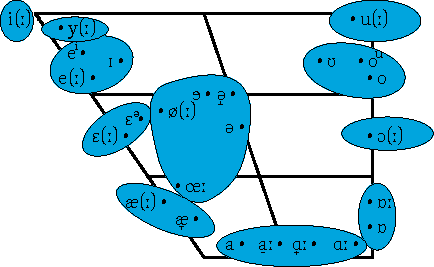
\includegraphics[width=.8\textwidth]{graphics/vowelcharts/bothoa-oral-vowels}
    \caption{Phonologically oral vowels in Bothoa Breton: principal allophones}
  \label{fig:bothoa-oral-vowels}
\end{figure} In the absence of actual formant data, the figure should be considered purely illustrative. Nevertheless, it does capture some of the extent of variation found in the dialect. (All the vowel charts in this section are adapted from \citeauthor{humphreys95:_phonol_bothoa_saint_nicol_pelem} \cite*{humphreys95:_phonol_bothoa_saint_nicol_pelem}, p.~73.)

\subsubsection{Nasal vowels}
\label{sec:nasal-vowels}

The dialect of Bothoa has six nasal vowels. According to \citet{humphreys95:_phonol_bothoa_saint_nicol_pelem}, nasal vowels are phonetically distinct from contingently nasalized vowels, which realize phonologically oral vowels adjacent to nasal consonants; presumably this corresponds to something like the difference between nasal vowels in French and nasalized vowels in English \citep{cohn90:_phonet,cohn93:_nasal_englis}.

All nasal vowels except \ipa{/ã/} do not enter into length contrasts. That is, long and short nasal vowels (except \ipa{/ã/}) are not used to implement lexical contrast, and phonetically long nasal vowels do not attract stress as long oral vowels do (\cref{sec:nasal-vowels-1}).

The high front nasal vowel \ipa{[ĩ]} is a nasalized version of cardinal \ipa{[i]}. It appears in about a dozen words, and occasionally the relevant lexical items can have oral \ipa{[i]} instead.

\ex.\a.\a.[]\twe{[ˈhĩːʃəw]}{henchoù}{roads}
\z.\b.\a.\twe{[ˈhĩːʒal]}{hejañ}{shake}
\b.\mbi{[ˈhiʒal]}

The mid-high nasal vowel \ipa{/ẽ/} is attested in about twenty lexical items. It is realized as a slightly dipthongized vowel \ipa{[ẽ\textsuperscript{ĩ}]}, in parallel with the diphthongized realization of long \ipa{/eː/} as \ipa{[e\textsuperscript{i}]}.

\ex.\a.\twp{ˈkwẽ\textsuperscript{ĩ}\kern-1pt vo}{koeñviñ}{to swell}
\b.\twp{ˈblẽ\textsuperscript{ĩ}\kern-1pt ʒal}{bl\^ejal}{moo}

The low front nasal vowel \ipa{[æ̃]} corresponds to the modern French pronunciation of the vowel in words such as \emph{bain}. It is overwhelmingly attested in borrowings from French.

\ex.\a.\twe{[ˈtræ̃]}{tren}{train (French \emph{train})}
\b.\twe{[ˈbasæ̃]}{basin}{pond; pool; bowl (French \emph{bassin})}


The front rounded nasal vowel \ipa{[ø̃]} is found in about a dozen lexical items. In a few words it alternates freely with an oral \ipa{[ø]}.

\ex.\a.\a.[]\twe{[ˈzø̃ːn]}{sizhun}{week}
\z.\b.\a.\twe{[ˈmøːz̥]}{meuz}{dish, delicacy}
\b.\mbi{[ˈmø̃ːz̥]}

The back mid rounded nasal vowel \ipa{/õ/} is described as significantly lower than the nasalized allophone of the mid high vowel \ipa{[o]}. It is attested in around twenty lexical items, but it is also used in borrowings from French.

\ex.\a.\twp{ˈpɔ̃ːʃəw}{ponchoù}{bridges}
\b.\twp{tɔ̃ːj̃\kern-1pt əw}{tonioù}{tunes}

Finally, the low nasal vowel \ipa{/ã/} is amply attested not only in roots, but in a number of productively used suffixes, and accounts for the vast majority of nasal vowel tokens. It is described as the nasalized correspondent of the back low unrounded vowel \ipa{[ɑ]}.

\ex.\a.\twp{ˈmɑ̃m}{mamm}{mother}
\b.\twp{ˈbrasɑ̃}{brasañ}{biggest}

It has a dipthongized allophone \phonint{ɑ̃\textsuperscript{õ}}, used word-finally in stressed position and, by some speakers, before the sequence of \phonint{ŋ} and a dorsal stop.

\ex.\a.\a.\twp{klɑ̃\textsuperscript{õ}}{klañv}{ill}
\b.\twp{ˈhɑ̃\textsuperscript{õ}}{hañv}{summer}
\z.\b.\a.\twp{ˈstɑ̃ŋɡ̊}{stank}{pond}
\b.\mbp{ˈstɑ̃\textsuperscript{õ}ŋɡ̊}

The low vowel is the only nasalized vowel to enter a length contrast, as the following examples demonstrate.

\ex.\a.\twp{ˈlɑ̃n}{lann}{gorse bush}
\b.\twp{ˈlɑ̃ːn}{leun}{full}

The set of nasal vowels in the dialect is shown in \cref{fig:bothoa-nasal-vowels}.

\begin{figure}[htp]
  \centering
  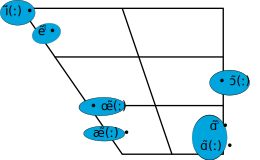
\includegraphics[width=.8\textwidth]{graphics/vowelcharts/bothoa-nasal-vowels}
  \caption{Nasal vowels in Bothoa Breton}
  \label{fig:bothoa-nasal-vowels}
\end{figure}

\subsubsection{Diphthongs}
\label{sec:diphthongs}

\citet{humphreys95:_phonol_bothoa_saint_nicol_pelem} identifies the following diphthongs in the Bothoa dialect: \phonint{ɛĭ}, \phonint{əy̆}, \phonint{əŭ} or \phonint{æŭ} (depending on the speaker), \phonint{aŭ}, and \phonint{ɑ̃w̃}. These are exemplified below.

\ex.\a.\a.[]\twp{ˈsɛĭz̥}{seizh}{seven}
\z.\b.\a.[]\twp{ˈəy̆n}{evn}{bird}\footnote{This word, along with its plural \phonint{ˈəy̆nəd̥}, is the only example of this diphthong in the dialect    \citep[p.~120]{humphreys95:_phonol_bothoa_saint_nicol_pelem}.}
\z.\b.\a.\twp{ˈdəŭ}{daou}{two (m.)}
\b.\mbp{ˈdæŭ}
\z.\b.\a.[]\twp{ˈdaŭr}{dour}{water}
\z.\b.\a.[]\twp{ˈdɑ̃w̃ʒər}{tavañjer}{apron}


\begin{figure}[htp]
  \centering
  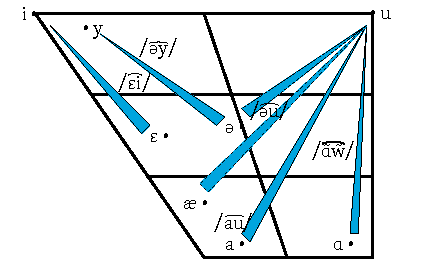
\includegraphics[width=.8\textwidth]{graphics/vowelcharts/bothoa-diphthongs}
  \caption{Diphthongs in Bothoa Breton}
  \label{fig:bothoa-diphthongs}
\end{figure}

\subsection{Consonants}
\label{sec:consonants-3}

The  phonetic inventory of consonants attested in Bothoa Breton is shown in \cref{tab:bothoa-cons-phonet},  which reproduces (with typographic changes) the table given by \citet[p.~123]{humphreys95:_phonol_bothoa_saint_nicol_pelem} and shows the set of \emph{phonetic} segments, \ie it lists the symbols needed in a narrow transcription.

\begin{sidewaystable}
  \centering
  \begin{tabular}{lccccccccccccc}
      \toprule
      & \multicolumn{2}{c}{Labial} & \multicolumn{4}{c}{Coronal} & \multicolumn{2}{c}{Palatal} &  &  &  &  \\
      \cmidrule{2-3}\cmidrule{4-7}\cmidrule{8-9}
      Manner & \hypcell[4em]{Labio\-dental} & Bilabial & Dental & Alveolar & \hypcell[4em]{Palato\-alveolar} & \hypcell[4em]{Alveo\-palatal} & Palatal &       \hypcell[4em]{Palatal-labial}  & Velar & Uvular & Pharyngeal & Glottal \\
      \midrule
      Stop & & \ipa{p~b} & \ipa{t~d} & & & \ipa{tʲ~dʲ} & \ipa{c~ɟ} & & \ipa{k~ɡ} \\
      Affricate & & & & & & \ipa{tɕ~dʑ} \\
      Fricative & \ipa{f~v} & & & \ipa{s~z} & \ipa{ʃ~ʒ} & \ipa{ɕ~ʑ} & \ipa{ç~j} & & \ipa{x~ɣ} & \ipa{\phantom{χ}~(ʁ)} & \ipa{ħ} & \ipa{h~ɦ} \\
      Nasals & \ipa{ɱ} & \ipa{m~m̥} & \ipa{n~n̥} & & & \ipa{ɲ~ɲ̥} & \ipa{j̃} & & \ipa{ŋ~ŋ̊} \\
      Laterals & & & \ipa{l~l̥} \\
      Rhotics & & & & \ipa{r~r̥} \\
      Approximants & & \ipa{w~w̥} & & & \ipa{j̃} & \ipa{ç~j} & & \ipa{ɥ} & & \ipa{(χ̞)~(ʁ̞)} \\
\bottomrule
  \end{tabular}
  \caption{Consonants: phonetic inventory}
  \label{tab:bothoa-cons-phonet}
\end{sidewaystable}

\subsubsection{The phonetic realization of consonants}
\label{sec:phon-real-cons}

The stops \ipa{[p~t~k]} and \ipa{[b~d~ɡ]} and the affricate pair \ipa{[ʧ~dʒ]} are distinguished by  voicing; the voiceless stops are said to lack noticeable aspiration (\foreigntextquote{french}{sans aspiration notable}).\footnote{The phonetic study of the west Cornouaillais dialect of Argol by \citet{Bot82} also shows full voicing of stops.} Minimal pairs are shown in \cref{ex:bothoa-voicing-minpairs}.

\ex.\label{ex:bothoa-voicing-minpairs}\a.\a.\twp{ˈboɫx}{boulc'h}{first cut}
\b.\twp{ˈpoɫx}{polc'h}{bug}
\z.\b.\a.\twp{ˈdiː}{div}{two (f.)}
\b.\twp{ˈtiː}{ti}{house}
\z.\b.\a.\twp{ˈɡãːnət}{ganet}{born}
\b.\twp{ˈkãːnət}{kanet}{sung}

The velar stops \ipa{[k~ɡ]} have fronted allophones, which \citet{humphreys95:_phonol_bothoa_saint_nicol_pelem} writes as \ipa{[c~ɟ]} and describes as \enquote{mediopalatal} (\textfrench{\emph{médio-palatale}}). These are found before the segment \ipa{[i]}. I assume they represent the same phonological segment as \ipa{[k]} and \ipa{[ɡ]} and thus will transcribe them as \ipa{[kʲ~ɡʲ]}. The main reason is that there no evidence for a phonological distinction between \ipa{[k~ɡ]} and \ipa{[kʲ~ɡʲ]}. The decision is also supported by the fact that nasals are realized as \phonint{ŋ} and not \phonint{ɲ} before these segments. Some examples are given in \ref{ex:bothoa-ki-exx}.

\ex.\label{ex:bothoa-ki-exx}\a.\twp{ˈlakʲiãm}{lakiamp}{we will put}
\b.\twp{akʲ i ˈziː}{hag he zi}{and her house}
\b.\twp{ˈvrãŋkʲiz̥}{frankiz}{open space, the outdoors}
\b.\twp{ˈklɒːɡʲiad̥}{klogiad}{ladleful}

The affricates \phonint{tɕ} and \phonint{dʑ} are described as similar to the  Polish orthographic \emph{\'c}, \emph{d\'z}. I will use the symbols \ipa{[ʧ~dʒ]} throughout for convenience.

\ex.(Near-)minimal pairs for velars
\a.\a.\twp{ˈʧɛĭsə}{keid-se}{so far}
\b.\twp{ˈkɛĭn}{kein}{back}
\z.\b.\a.\twp{ˈdʒaz̥}{degas}{bring}
\b.\twp{ˈɡaz̥}{gas}{send (mutated form)}

\label{bothoa-phonetic-palatalization}Segments acoustically similar to \phonint{ʧ} and \phonint{dʒ} may also appear as the extremes of a continuum of variable realizations corresponding to the sequence of a coronal stop and the vowel \ipa{[i]} before another vowel, as in \cref{ex:bord}.

\ex.\label{ex:bord}\a.\a.\twp{ˈbɒrd̥}{bord}{side}
\b.\twp{ˈbɒrdʒəw}{bordoù}{sides}
\b.\mbp{ˈbɒrdiəw}
\z.\b.\label{ex:rastel-kontel}\a.\twp{ˈkonˌtɛl}{kontel}{knife}
\b.\twp{ˈkontiəw}{kontilli}{knives}
\b.\mbp{ˈkontjəw}
\b.\mbp{ˈkonʧəw}


The fricatives \ipa{[f~v]}, \ipa{[s~z]} and \ipa{[ʃ~ʒ]} are said to be similar to their French counterparts. \mbox{(Near-)}minimal pairs are given in the examples below.

\ex.\a.\a.\twp{ˈvãmin}{binim}{venom}
\b.\twp{ˈfãmin}{famin}{hunger}
\z.\b.\a.\twp{ˈzel}{sell}{look}
\b.\twp{ˈsel}{}{(bike) saddle (French \emph{selle})}
\z.\b.\a.\twp{ˈʒakəz̥}{Jakez}{oaf}
\b.\twp{ˈʃakəd̥}{choked}{crumpled}


In preconsonantal contexts, \ipa{/s/} (or \ipa{/z/}) may alternate with \ipa{[h]} (phonetically normally \phonint{ħ} in this position). This is especially frequent with the prefix \preff{diz} (\preff{dis}).

\ex.\label{dislivan-dismantran}\a.\a.\twp{ˌdisˈliːvo}{dislivañ}{discolour}
\b.\mbp{ˌdiħˈliːvo}
\z.\b.\a.\twp{ˈdiħmɑ̃nt}{dismantrañ}{waste}
\b.\mbp{ˈdismɑ̃nt}

The alternation does not appear to be systematic, but is lexicalized in one case.\footnote{According to \citet[p.~168]{humphreys95:_phonol_bothoa_saint_nicol_pelem}, neither *\phonint{ˈr̥ɑːx} nor *\phonint{ˈr̥ɑːzəd̥} are possible in the dialect.}

\ex.\a.\twp{ˈr̥aːz̥}{razh}{rat}
\b.\twp{ˈr̥aːɦəd̥}{razhed}{rats}


The fricatives \ipa{[ʃ]} and \ipa{[ʒ]} do not appear to participate in variation with coronal fricatives parallel to that shown in \cref{ex:bord}, as shown in \cref{ex:morzel-brezel}.

\ex.\label{ex:morzel-brezel}\a.\twp{ˈmɒrˌzɛl}{morzhol}{hammer}
\b.\twp{ˈmɒrziəw}{morzholioù}{hammers}
\b.\mbp{ˈmɒrzjəw}
\b.*\mbp{ˈmɒrʒəw}

The fricative that \citet{humphreys95:_phonol_bothoa_saint_nicol_pelem} transcribes phonologically as \ipa{[h]} has a number of realizations. The voiceless glottal phonation \phonint{h} is found word-initially, word-medially following \ipa{[l~r]}, and immediately before the vowel bearing the main stress. The breathy voiced phonation \phonint{ɦ} is normally found intervocalically, and occasionally word-initially. The voiceless velar fricative \phonint{x} is found utterance-finally and before a voiceless consonant, while its voiceless correspondent \phonint{ɣ} is a rare variant noted word-finally in sandhi before \ipa{[m~v]}. Finally, the pharyngeal \phonint{ħ} is the most common preconsonantal variant, alternating freely with \phonint{x} and \phonint{ɣ}. Examples are given in \cref{ex:bothoa-h-exx}.

\ex.\label{ex:bothoa-h-exx}\a.\a.\twp{ˈhɛĭ}{heiz}{barley}
\b.\twp{ˈmarhəw}{marc'hoù}{stallions}
\z.\b.\a.\twp{ˈzɛɦo}{sec'hañ}{to dry}
\b.\twp{o ˈzaːɦ e}{ur sac'h eo}{(it) is a bag}
\z.\b.\a.\twp{o ˈplɑːx}{ur plac'h}{a girl}
\b.\twp{o ˌplɑːx ˈpəŭr}{ur plac'h paour}{a poor girl}
\z.\b.\a.\twp{ə ˈvjɒɣmə}{ar vuoc'h-mañ}{this cow}
\z.\b.\a.\twp{dæħˈmɑːt}{dalc'hmat}{always}
\b.\twp{o ˌvjɒħ ˈlart}{ur vuoc'h lart}{a fat cow}

\enquote{Occasionally} this fricative may also alternate with \ipa{[s]} (the precise nature of the variation is not described). The pattern is reminiscent
of that described above for \ipa{[s]} and \ipa{[z]} (as in \cref{dislivan-dismantran}).

\ex.\a.\a.\twp{ˈzɛːx}{sec'h}{dry}
\b.\twp{ˈzɛstər}{sec'hder}{dryness}
\b.\mbp{ˈzɛħtər}
\z.\b.\a.\twp{ˌdɛstəˈnoːs}{dec'h-da-noz}{tonight}
\b.\twp{dɛːx}{dec'h}{today}

The nasals \ipa{[m]} and \ipa{[n]} do not present significant difficulties. The nasal \ipa{[ŋ]} is only encountered before velar stops.

\ex.\a.\a.\twe{[ˈmãn]}{mann}{nothing}
\b.\twe{[ˈnãn]}{nann}{no}

The segment that \citet{humphreys95:_phonol_bothoa_saint_nicol_pelem} interprets as a phonological palatal nasal \ipa{[ɲ]} is realized as \phonint{ɲ} word-medially following \phonint{r} and \phonint{j}; in all other contexts, it is realized as a nasalized palatal glide \phonint{j̃\kern-1pt}, and these two segments are in free variation following \ipa{[w]}. Neither is found word-initially.

\ex.\a.\twp{ˈpwiːj̃\kern-1pt al}{poaniañ}{to upset}
\b.\twp{ˈkɛjɲəw}{keinioù}{backs}
\b.\twp{ˈtõj̃\kern-1pt əw}{tonioù}{tunes}
\b.\twp{ˈhãwɲo}{anvel}{to call, name}
\b.\mbp{ˈhãwj̃\kern-1pt o}


The phonetic segment \phonint{ɲ} can also appear as the member of a continuum of possible realizations, from \ipa{[ni]} through \ipa{[nj]} and \ipa{[nʲ]} to \ipa{[ɲ]}, as in \cref{binied}.

\ex.\label{binied}\a.\twp{ˈbiːniəd̥}{benniget}{blessed}
\b.\mbp{ˈbiːnĭəd̥}
\b.\mbp{ˈbiːnjəd̥}
\b.\mbp{ˈbiːɲəd̥}


The lateral \ipa{[l]} is normally similar to the French \ipa{[l]}. It demonstrates minor coarticulation effects. Specifically, the initial portion of the sonorant may be devoiced following voiceless stops (consistent with the description of voiceless stops as short-lag VOT segments). The lateral is slightly palatalized before \ipa{[i]} and slightly velarized before \ipa{[u]}. A more strongly velarized \ipa{[ɫ]} is found before \phonint{h} and \phonint{x}, as shown in \cref{ex:bothoa-dark-l}.\footnote{The association between \ipa{[h]} and velarized \phonint{ɫ} should perhaps be compared to the possible realization of \ipa{[rh]} as \phonint{xː} (see \cref{erch-chwech}). The class of \ipa{[h]} and (coda) \ipa{[l~r]} as velarized consonants (which may also exert a backing influence on preceding vowels) is reminiscent of the Old English \enquote{breaking}, \ie the appearance of a back glide before \ipa{[h]} (phonetically \phonint{h} and \phonint{x}) and coda \ipa{[l]} and \ipa{[r]}; see \citet[§§5.16\endash5.34]{hogg92:_old_englis}. It appears that breaking did not play an important rôle in the synchronic phonology of Old English \citep[§5.32]{hogg92:_old_englis}, but the precursors to the sound change may have been similar to the situation seen in Breton.}

\ex.\label{ex:bothoa-dark-l}\a.\twp{ˈbɔɫx}{boulc'h}{first cut}
\b.\twp{ˈmɔɫhəd̥}{moualc'hoù}{swallows}

The rhotic, for which I used the cover symbol \ipa{[r]}, is realized in a variety of ways. In the conservative variety (speakers born before 1920), it is normally an apical tap or trill, with the tap being the dominant pronunciation and the trill only found word-initially. It can be voiceless, especially following an initial voiceless stop. In newer varieties, it is realized either as a uvular fricative \ipa{[ʁ]}, or as a uvular approximant \ipa{[ʁ̞]} (also possibly devoiced to a relatively frictionless \ipa{[χ̞]}).

The approximants \ipa{[w~j~ɥ]} are described as generally similar to the corresponding French sounds as in \emph{oiseau}, \emph{hier}, \emph{huit}. They are slightly devoiced following voiceless consonants.

Finally, Bothoa Breton possesses a set of voiceless sonorants \ipa{[m̥~n̥~l̥~r̥~w̥~ɥ̊]}. In addition, \ipa{[ç]}, as we shall see below, stands in the same relationship to \ipa{[j]} as voiceless sonorants do to voiced ones. The phonetic realization of these segments was studied by \citet{humphreys}. He found that \ipa{[m̥]}, \ipa{[n̥]} and \ipa{[l̥]} can be broken up into a voiceless and a voiced portion, so \phonint{m̥m}, \phonint{n̥n} and \phonint{l̥\kern-1pt l}. The palatal-labial voiceless glide \ipa{[ɥ̊]} is extremely rare; the voiceless palatal \ipa{[ç]} is described as similar to the German \emph{ich-Laut}, and \ipa{[w̥]} is said to be similar to the \ipa{[ʍ]} of certain English dialects. Finally, the realization of \ipa{[r̥]} varies: some speakers have a voiceless tap or trill \phonint{r̥} similar to Welsh \emph{rh}, and others have a uvular fricative \phonint{χ}.

\subsubsection{Word-final phonetics and sandhi}
\label{sec:word-final-phonetics}

The realization of consonants, and especially obstruents, in phrasal contexts is often different from that found in lexical contexts; this is particularly true in utterance-final position. The phonetic alternations can be broadly classified into two groups: lack of release and loss of laryngeal specification.

\paragraph{Lack of release}
\label{sec:lack-release}

Word-final stops, whether before a pause or before another consonant, are often unreleased, which can even lead to confusion as to the identity of the final stop:

\ex.\a.\a.[]\twp{ˈdib̥̚}{dibr}{saddle}
\z.\b.\a.[]\twp{o ˈhad̥̚}{ur c'had}{a hare}
\z.\b.\a.[]\twp{ˈɡwɑːɡ̊̚}{gwak}{weak}
\z.\b.\a.\twp{ˈr̥iːdəɡ̊̚}{redek}{run}
\b.\mbp{ˈr̥iːdəd̥̚}


In word-final nasal\endash stop sequences, not only can the stop remain unreleased, but also the nasal may be realized with greater duration. If an underlyingly voiceless stop is deleted or obscured in this manner, the nasal is also often, though not necessarily, voiceless (except before a voiced segment). The appearance of stops is especially disfavoured before another consonant

\ex.\label{bothoa-pont-et-al}\a.\a.\twp{o ˈpont}{ur pont}{a bridge}
\b.\mbp{o ˈpont̚}
\b.\mbp{o ˈpon̥}
\b.\mbp{o ˈponː}
\b.\twp{o ˌponː ˈkoːz̥}{ur pont kozh}{an old bridge}
\b.\mbp{o ˌpon ˈkoːz̥}
\z.\b.\a.\twp{ˈdɛnt}{dent}{teeth}
\b.\twp{ˌdɛn ˈbrɑː}{dent brav}{good teeth}
\b.\mbp{ˌdɛnː ˈbrɑː}
\z.\b.\a.\twp{on ˈdɑ̃nd al}{un dant all}{another tooth}
\b.\mbp{on ˈdɑ̃nː al}

A similar phenomenon involving the loss of the stop articulation and a lengthening of the preceding consonant is found in obstruent sequences, in practice limited to sequences of \ipa{[s]} and a stop:

\ex.\a.\a.[]\twp{ˈtrist e}{trist eo}{[it] is sad}
\z.\b.\a.\twp{ˌlɒst ˈhiːr}{lost hir}{a long tail}
\b.\mbp{ˌlɒsː ˈhiːr}
\b.\mbp{ˌlɒs ˈhiːr}
\z.\b.\a.\twp{ˈʒist}{chistr}{cider}
\b.\mbp{ˈʒisː}
\z.\b.\a.\twp{ˈʒisː ˈkaləd̥}{chistr kalet}{hard cider}
\b.\mbp{ˈʒis ˈkaləd̥}


Final coronal stops may disappear from the acoustic record before another consonant: this is said to be obligatory in unstressed syllables (\cref{ex:evid-mirout-boued}) and \enquote{sporadic} in stressed ones (\cref{ex:koad-lokeltaz}).

\ex.\label{ex:evid-mirout-boued}\a.\twp{vid̥}{evit}{for, in order to}
\b.\twp{miːrəd̥}{mirout}{keep, look after}
\b.\twp{vi ˌmiːrə ˈbwid̥}{evit mirout boued}{in order to watch the food}

\ex.\label{ex:koad-lokeltaz}\a.\twp{ˈkwɛd̥}{koad}{forest}
\b.\twp{ˌkwɛ loɡəˈtaːz̥}{koad Lokeltaz}{the forest of Locqueltas}

When two identical consonants straddle a word boundary, the result is either a \enquote{slightly geminated} articulation when both consonants belong to stressed syllables (\cref{ex:koad-derv}); in other positions the result is said to be indistinguishable from a single consonant (\cref{ex:ar-parrez-se}).

\ex.\a.\label{ex:koad-derv}\a.\twe{/kwæd/}{koad}{wood}
\b.\twp{ˌkwædˈdær}{koad derv}{oak}
\z.\b.\label{ex:ar-parrez-se}\a.\twe{/paruz/}{parrez}{parish}
\b.\twp{ə ˈbarusə}{ar barrez-se}{this parish}

\paragraph{Laryngeal phenomena}
\label{sec:laryngeal-phenomena}

Word-finally, the contrast between voiced and voiceless obstruents is suspended. However, the outcome of this suspension depends on the phonetic context.

\subparagraph{Final laryngeal neutralization}
\label{sec:final-laryng-neutr-phon}

I use the term \enquote{final laryngeal neutralization} \citep[\cfm][]{iverson11:_final} to refer to the fact that both voiced and voiceless obstruents exhibit what \citet[p.~190]{humphreys95:_phonol_bothoa_saint_nicol_pelem} calls the \enquote{voiceless realization} before a pause (\ie phrase-finally). Fully voiced obstruents are entirely absent from this position. However, according to \citet{humphreys95:_phonol_bothoa_saint_nicol_pelem}  the actual realization is not necessarily identical to that of true voiceless obstruents:

\blockquote{It should be pointed out that the alternation between voiced and voiceless segments, which represents the most important category of these [sandhi] modifications, is, from the phonetic point of view, not a simple binary choice: quite often one encounters not just voiceless lenes, but also consonants with a decrease in voicing. The faster the speech rate and the more relaxed the articulation, the more pronounced are the assimilations.\footnote{\foreigntextquote{french}{Il faut se rappeler [\ldots] que l'alternance sourde/sonore, qui représente la catégorie plus importante de ces modifications, n'est pas, sur le plan phonétique, un simple choix binaire: on rencontre assez souvent, non seulement des sourdes douces, mais aussi des consonnes à sonorité décroissante. Plus le débit rapide et l'articulation relâchée, plus les assimilations sont poussées.}}}

Of course, only instrumental study could clarify the correctness, and in fact the true empirical content of this description. Still, the realization of obstruents devoiced by sandhi is apparently nor identical to that of lexical voiceless obstruents. Consequently, I use the devoicing diacritic for prepausal obstruents in both phonetic and surface\hyp phonological transcription. (Phonological arguments for a distinction are provided below, see especially \cref{sec:except-devo-sandhi}.) Two examples are shown in \ref{ex:bothoa-findev}, together with forms without neutralization which demonstrate the underlying laryngeal specification:

\ex.\label{ex:bothoa-findev}\a.\a.\twp{ˈkɔɡ̊}{kog}{rooster}
\b.\twp{ˈkɔɡəw}{kogoù}{forests}
\z.\b.\a.\twp{ˈtɔɡ̊}{tog}{hat}
\b.\twp{ˈtɔkəw}{togoù}{hats}

\subparagraph{Sandhi voicing}
\label{sec:sandhi-voicing-phon}

When an obstruent is not final in the phrase and is followed by a sonorant, a vowel, or a voiced obstruent, it is generally realized with voicing irrespective of its underlying laryngeal specification. Examples of this are shown in \cref{ex:bothoa-sandhi-voi}.

\ex.\label{ex:bothoa-sandhi-voi}\a.\a.\twp{kɔɡ̊}{kog}{rooster}
\b.\twp{o ˌhɔk ˈtrøt}{ur c'hog treut}{a skinny rooster}
\b.\twp{ˌkɔɡ izˈmaːj}{kog If-Mai}{Yves-Marie's rooster}
\z.\b.\a.\twp{tɔɡ̊}{tog}{hat}
\b.\twp{on ˌtɔk ˈʃik}{un tog chik}{a chic hat}
\b.\twp{on ˈtɔɡ ˌal}{un tog all}{another hat}
\b.\twp{ˌtɔɡ ˈʒãː}{tog Yann}{Jean's hat}

\enquote{Quite often} (\foreigntextquote{french}{assez souvent}) the underlying voiceless fricatives \ipa{/f/}, \ipa{/s/}, and \ipa{/ʃ/}, when preceded by short vowels, resist the voicing in the relevant context. It is not clear whether this resistance is a property of lexical items or whether the same lexical item can appear in both forms. \citet{humphreys95:_phonol_bothoa_saint_nicol_pelem} says that examples like those in \cref{ex:bothoa-vcl-fricative-voicing} \enquote{coexist} with those in \cref{ex:bothoa-vcl-fricative-no-voicing} (all the relevant words end in lexical voiceless obstruents).

\ex.\a.\label{ex:bothoa-vcl-fricative-voicing}\a.\twp{o ˈprøz wæ}{ur pres a oa}{it was a cupboard}
\b.\twp{o ˈpeʒ laˈpiːnəd̥}{ur pech lapined}{a rabbit trap}
\z.\b.\label{ex:bothoa-vcl-fricative-no-voicing}\a.\twp{on ˈtas wæ}{un tas a oa}{it was a cup}
\b.\twp{on ˈhaʃ ˈlem}{un hach lem}{a well-sharpened axe}

As for final consonant sequences, \citet[p.~196]{humphreys95:_phonol_bothoa_saint_nicol_pelem} distinguishes three types of realizations before vowels:

\begin{itemize}
\item If the first element is a liquid,  word-final obstruents behave exactly as if they followed a vowel.
\item In the case of sequences of the type \enquote{nasal + stop}, the situation is complicated by the fact that, as discussed above (see \cref{bothoa-pont-et-al} on p.~\pageref{bothoa-pont-et-al}), these tend to undergo some sort of progressive assimilation in terms of nasality, losing the burst. Nevertheless, as that example shows, if the stop is not deleted or obscured in such sequences, it can be realized with voicing.
\item In sequences of the type \enquote{\ipa{/s/} + stop} (where the majority are of the form \ipa{/st/}), dropping of the final consonant is common (especially before a consonant, as is the case for stops generally). Interestingly, even if the stop disappears from the acoustic record, pre-sonorant (or at least prevocalic) voicing of such sequences is quite uncommon: while realizations like that in \cref{ex:chistr-all} do exist, \citet{humphreys95:_phonol_bothoa_saint_nicol_pelem} attributes them to changes in the underlying form (so that \eg `cider' is underlyingly \ipa{/ʒis/} rather than \ipa{/ʒist/}). However, voicing assimilation is possible before obstruents. The segment \ipa{[h]} inhibits pre-sonorant voicing.

\end{itemize}

\ex.\a.\a.\twp{ˈlɒst}{lost}{tail}
\b.\twp{ˈlɒst ˈhiːr}{lost hir}{long tail}
\b.\mbp{ˈlɒsː ˈhiːr}
\b.\twp{o ˌlɒzd ˈbɛːr}{ul lost berr}{a short tail}
\b.\mbp{o ˌlɒzː ˈbɛːr}
\b.\mbp{o ˌlɒz ˈbɛːr}
\z.\b.\a.\twp{ˈʒist}{chistr}{cider}
\b.\mbp{ˈʒisː}
\b.\twp{ˌʒis ˈkalət}{chistr kalet}{strong cider}
\b.\mbp{ˌʒisː ˈkalət}
\b.\label{ex:chistr-all}\twp{ˈʒiz ˈal}{chistr all}{another cider}
\z.\b.\a.\twp{ˈtrist}{trist}{sad}
\b.\twp{ˈtrist e}{trist eo}{[it] is sad}

\paragraph{Miscellaneous sandhi changes}
\label{sec:misc-sandhi-chang}

Other postlexical alternations are possible, but are described as irregular.

Final obstruents may be fully or partially nasalized before other nasals:

\ex.\a.\twp{ˈzæːb̥}{sabl}{sand}
\b.\twp{ˌzæːb ˈnæd e}{sabl naet eo}{(it) is proper sand}
\b.\mbp{ˌzæːm ˈnɛd e}

The affricates may lose their fricative portion before a consonant to be realized as something like palatalized coronal (\cref{ex:bothoa-ts-to-t}) or dorsal (\cref{ex:bothoa-ts-to-k}) stops.

\ex.\a.\label{ex:bothoa-ts-to-t}\a.\twp{ˌʧitʲ ˈpwɛːz̥}{kig poazh}{roasted meat}
\b.\twp{ˌʧidʲ ˈbærəd̥}{kig berved}{boiled meat}
\z.\b.\label{ex:bothoa-ts-to-k}\a.\twp{ˌʧiɡ ˈɡad̥}{kig gad}{hare meat}
\b.\twp{ˌʧik ˈr̥ɒstəd̥}{kig rostet}{roasted meat}

Very sporadically, underlying \ipa{/s/} and \ipa{/z/} may be realized as \ipa{[h]} before a sonorant (recall that this can also happen lexically):

\ex.\a.\a.\twp{ˈhõz̥}{honnezh}{this one there}
\b.\twp{ˌhõh wæ ˈbraːz̥}{honnezh a oa braz}{it was big}
\z.\b.\a.\twp{ˈmeməz̥}{memes}{same}
\b.\twp{ˌmemə m̥\kern1pt ɔd̥}{memes mod}{the same way}



\subsection{Phonological inventories}
\label{sec:phon-invent}

The phonemicization of Bothoa Breton segments appears mostly straightforward. In this section I discuss some outstanding issues.


\subsubsection{The status of the schwa}
\label{sec:status-schwa}

The phonemic status of the distinction between \ipa{[ə]} and \ipa{[ø]}/\ipa{[œ]} is difficult to determine, which is similar to the situation in French. It is certainly not used to implement lexical contrast, since the segments stand in (almost) complementary distribution: there is one instance (secondary stress on final syllables) where different speakers use different phones (some use a more like \ipa{[ø]}-like segment in this position). The complementary distribution could in principle be due either to \ipa{[ə]} and \ipa{[ø]} being two different phonological symbols (in which case the inter-speaker variation in the case of final syllables could be due to some phonological difference in how that position is represented) or to a language\hyp particular aspect of phonetic implementation.

Arguments for the former view are difficult to come by, since both \phonint{ə} and (especially) \phonint{œ} are quite inert phonologically. The only argument for a phonological distinction is its categoricity. However, categorical distributions in the data may well arise from non-phonological factors (\cref{sec:relev-categ-distr}). Moreover, in the absence of instrumental data we cannot  say for sure that the distinction is implemented categorically: in fact, given the relatively wide range of possible phonetic realizations of \ipa{[ə]} (cf.\ \cref{fig:bothoa-oral-vowels} on p.~\pageref{fig:bothoa-oral-vowels}), it appears possible that the realizations of \ipa{[ø]} and \ipa{[ə]} may actually be forming a continuum.

The evidence is thus indeterminate.\footnote{\citet[p.~108]{humphreys95:_phonol_bothoa_saint_nicol_pelem} treats \ipa{[ø]} and \ipa{[ə]} as a single phoneme, on the basis of the complementary distribution. He also observes that when the melody in a song requires prolonging a syllable with a schwa, Bothoa speakers will use a front rounded vowel (he notes that speakers to the west of Bothoa use \ipa{[ɛ]} in similar situations). However, it is not entirely clear whether these facts are linguistically relevant. In particular, \citet{humphreys95:_phonol_bothoa_saint_nicol_pelem} transcribes the relevant example with a stress mark on the schwa-containing syllable: \phonint{kɑ̃ˈnøːːt} `sung' (normally \ipa{[ˈkãːnəd̥]}). I leave this matter aside here.} Moreover, there is a distinct possibility that, given the absence of strong evidence either way, different learners may actually converge on different mental grammars that would both be relatively well compatible with the relevant ambient data. In the absence of firm evidence for a phonological contrast, I follow \citet{humphreys95:_phonol_bothoa_saint_nicol_pelem} in treating \ipa{[ə]} and \ipa{[ø]} as the same phonological segment. I will transcribe it as \ipa{[ə]} in purely phonological contexts (\eg when describing feature specifications), but will keep \ipa{[ø]} in surface-phonological transcriptions of words to keep them closer to the phonetics.\footnote{A third potential solution is proposed by \citet{le00:_le_malguen} for the dialect of Malguénac, where similar facts obtain with respect to the complementary distribution of \phonint{œ} and \phonint{ə}: working in a structuralist framework, \citeauthor{le00:_le_malguen} proposes to treat surface \ipa{[ə]} as representing phonemic \ipa{/œ/} when there is evidence from alternations and as phonemic \ipa{/ə/} when the relevant vowel never alternates with \ipa{[œ]}. However, this solution again rests on a phonetic argument rather than a phonological one.}


\subsubsection{Consonants}
\label{sec:bothoa-consonant-dist}

The consonant inventory appears to be mostly unproblematic. The following remarks are in order:

\begin{itemize*}
\item The phonological segment that \citet{humphreys95:_phonol_bothoa_saint_nicol_pelem} transcribes as \ipa{/ɲ/} is realized as either \phonint{ɲ} or \phonint{j̃\kern-1pt}. Since \phonint{ɲ} can also be the realization of a \ipa{[ni]} sequence, I use \ipa{[j̃\kern-1pt]} in phonological transcription;
\item The rhotic has a range of coronal and uvular realizations varying across contexts and speakers. I use \ipa{[r]} throughout for simplicity;
\item I transcribe the affricates as \ipa{[ʧ]} and \ipa{[dʒ]} throughout, irrespective of their phonetic realization;
\item I ignore some assimilations that are clearly allophonic (\ie which do not involve changes of phonological symbols) such as the fronting of \ipa{[k]} and \ipa{[ɡ]} before front vowels;
\item I follow \citet{humphreys95:_phonol_bothoa_saint_nicol_pelem} in treating \ipa{[h]} as a single phonological symbol, despite the multitude of its realizations. Apart from the lack of phonological evidence, the reason for this decision is the fact that the variation is described as not being categorical, but rather appears to be driven by phonetic context.
\end{itemize*}

\Cref{tab:inventories-bothoa} shows the phonological inventories for Bothoa Breton I operate with in this thesis; the labels are to be taken as purely descriptive. For an explanation of the transcription of the voiceless sonorants, see \cref{sec:provection-sonorants}.

\begin{table}[htp]
\centering
\subtop[Vowel inventory]{%
  \begin{tabular}{lcccc}
    \toprule
& \multicolumn{2}{c}{Front} & Central & Back \\
\cmidrule{2-3}
Height & Unrounded & Rounded & & \\
\midrule
High & \ipa{i~iː} & \ipa{y~yː} & & \ipa{u~uː} \\
Mid-high & \ipa{e~eː} & & & \ipa{o~oː} \\
Mid & \ipa{ɛ~ɛː} & \ipa{ø~øː} & \ipa{ə} & \ipa{ɔ~ɔː} \\
Mid-low & \ipa{æ~æː} & & & \ipa{ɒ~ɒː} \\
Low & & & \ipa{a~aː} \\
\bottomrule
\label{tab:phonemic-vowels-bothoa}
  \end{tabular}%
}
\subtop[Consonant inventory]{%
  \begin{tabular}{lccccccc}
    \toprule
Manner & Labial & Coronal & Postalveolar  & \hypcell[4em]{Palatal\-labial} & Palatal & Dorsal & Glottal \\
\midrule
Stops & \ipa{p~b} & \ipa{t~d} & & &  & \ipa{k~ɡ} \\
Affricates & & & \ipa{ʧ~dʒ} \\
Fricatives & \ipa{f~v} & \ipa{s~z} & \ipa{ʃ~ʒ} & & & & \ipa{h} \\
Nasals & \ipa{m~hm} & \ipa{n~hn} & & & \ipa{j̃}  \\
Laterals & & \ipa{l~hl} \\
Rhotics & & \ipa{r~hr} \\
Approximants & \ipa{w~hw} & & & \ipa{ɥ~hɥ} & \ipa{j~hj} \\
\bottomrule
  \end{tabular}
}
  \caption{Inventories for Bothoa Breton}
\label{tab:inventories-bothoa}
\end{table}

In \cref{tab:transcription-bb} I summarize the transcription practice I use for surface\hyp phonological representations in this chapter.\begin{table}[tbp]
  \centering
  \adjustbox{width=\textwidth}{\begin{tabular}{*{2}{>{\ipafont}l}p{.6\textwidth}}
    \toprule
    Phonology & Phonetics & Comments\\
    \midrule
    {[p t ʧ k]} & \phonint{p t ʧ k(ʲ)} & Short-lag VOT, found word-finally only in exceptional cases \\
    {[b d dʒ ɡ]} & \phonint{b̬ d̬ d̬ʒ̬ ɡ̬(ʲ)} & Fully voiced stops, not found word\hyp finally \\
    {[b̥ d̥ d̥ʒ̊ ɡ̊]} &
    \begin{minipage}[t]{.2\linewidth}\raggedright
      \phonint{p/b̥/b(̚) t/d̥/d(̚) tʲ/d̥ʲ/dʲ/dʒ k/ɡ̊/ɡ(̚)}
    \end{minipage}
& Partially or fully voiced depending on context, possibly unreleased, found mostly word\hyp finally \\
    {[f s ʃ]} & \phonint{f s ʃ} & \\
    {[v z ʒ]} & \phonint{v̬ z̬ ʒ̬} & Fully voiced, not found word\hyp finally \\
    {[v̥ z̥ ʒ̊]} & \phonint{f/v̥/v s/z̥/z ʃ/ʒ̊/ʒ} & Partially or fully voiced depending on context, found word\hyp finally \\
    {[h]} & \phonint{h ɦ ħ ɣ} & Depending on context \\
    {[m n]} & \phonint{m n/ŋ} & No significant allophony described other than possible assimilation of \ipa{/n/} to \phonint{ŋ} \\
    {[l r]} & \phonint{l/ɫ ɾ/r/ʁ/χ} & Some velarization of \ipa{[l]}, between\hyp speaker variation in \ipa{[r]} \\
    {[j̃\kern-1pt]} & \phonint{j̃\kern-1pt{} ɲ} & Depending on context \\
    {[u/w i/j ɥ]} & \phonint{w j ɥ} & As with Welsh, I write \ipa{[w~j]} in onsets and \ipa{[i~u]} in nuclei despite the lack of a phonological distinction\\
    {[hm hn hl]} & \phonint{m̥\kern1pt m n̥n l̥\kern-1pt l/ɬ} & \multirow{2}{*}{See \cref{sec:provection-sonorants} for the phonological rationale}  \\
    {[hr hw hj hɥ]} & \phonint{r̥/χ ʍ ç ɥ̊} \\
    \bottomrule
  \end{tabular}
}  \caption{Transcription for Bothoa Breton}
  \label{tab:transcription-bb}
\end{table} In the next section I take up some issues in the suprasegmental phonology of Bothoa Breton, specifically stress, syllable structure, phonotactics, and the relationship between vowel length and laryngeal specification.

\section{Suprasegmental phonology}
\label{sec:supr-phon}

\subsection{Stress}
\label{sec:stress}

Unlike most other Brythonic varieties, in Bothoa Breton the placement of stress is not determined for the most part by top-down prosodic requirements. In this section I argue that stress placement in Bothoa Breton is mostly driven by lexical factors, mitigated by top-down requirements which include stressing the rightmost moraic trochee in a word and final-syllable stress.

\subsubsection{Types of stress}
\label{sec:types-stress}

According to \citet{humphreys95:_phonol_bothoa_saint_nicol_pelem}, stressed vowels are characterized by greater intensity, greater length and rising pitch (this latter especially pronounced on final syllables).

There is one type of words where the realization of stress is not entirely straightforward. According to \citet{humphreys95:_phonol_bothoa_saint_nicol_pelem}, there is a marked difference between two classes of disyllabic words, exemplified in \ref{ex:bothoa-double-peak}.

\ex.\label{ex:bothoa-double-peak}\a.\twe{[ˈpærson]}{person}{parson}
\b.\twe{[ˈdaˌvad̥]}{dañvad}{ewe}

If \posscite[']{humphreys95:_phonol_bothoa_saint_nicol_pelem} description is correct, in words of the first type intensity, length and pitch peaks all converge on the initial syllable. In words of the second type, however, it is said that both syllables are of the same length. Moreover, final syllables in these words bear an especially abrupt rise in pitch, with the result that the accentuation of word such as \ipa{[ˈdaˌvad̥]} `ewe' \enquote{rather strikingly resembles Welsh accentuation} (\foreigntextquote{french}{rappelle d'un façon assez frappante l'accentuation du gallois}); for discussion of stress in Welsh, \cf \cref{sec:pros-struct-stress}.

\citet{humphreys95:_phonol_bothoa_saint_nicol_pelem} interprets this additional prominence on final syllables as secondary stress. He notes, however, that the ordering of the main and secondary stress is not necessarily fixed:  such words may also surface with the second syllable more prominent than the first one, or with both syllables equally prominent (something that is also reminiscent of Welsh, see \cref{sec:gliding-as-phonetic}). \citet{humphreys95:_phonol_bothoa_saint_nicol_pelem} entertains an account where the contrast between the two types of words shown in \cref{ex:bothoa-double-peak} is really a contrast between words with one stress (\ipa{\'σσ}) and words with two stresses (\ipa{\'σ\'σ}), which I argue below to be correct.

The placement of secondary stress is generally unpredictable, so it is marked in the transcription. \citet{humphreys95:_phonol_bothoa_saint_nicol_pelem} also describes a \enquote{tertiary stress}, said to fall on peripheral syllables where they are separated from main stress by one or more unstressed syllables. Tertiary stress is \enquote{almost as perceptible as secondary stress}.\footnote{\foreigntextquote{french}{[P]resque aussi perceptible que l'accent secondaire.}} It is not marked in \posscite[']{humphreys95:_phonol_bothoa_saint_nicol_pelem} transcriptions, but below I provide some evidence that it must also be treated as phonological.

\subsubsection{Stress placement}
\label{sec:stress-placement}

I propose that stress placement in Bothoa Breton is lexical, with several qualifications:

\begin{itemize*}
\item Long vowels are always stressed;
\item Where possible, the stress foot is a moraic trochee;
\item If there are several feet in the word, the rightmost one bears the main stress.
\end{itemize*}

In words with only short vowels, stress can in principle fall on any syllable, with the exception of disyllables: as described above, possible patterns are at least \'LL and \'L\`L, where the latter has a range of possible realizations. \citet{humphreys95:_phonol_bothoa_saint_nicol_pelem} gives a few examples of \`L\'L forms, but since this pattern is also said to be a possible realization of \enquote{\'L\`L}, it is not entirely clear that tokens of \`L\'L are not in fact instances of \enquote{double-stressed} words for which \'L\`L variants have not been recorded as a matter of accident. \Crefrange{bothoa-ll}{bothoa-llll} show short-vowel-only patterns.

\ex.\label{bothoa-ll}Two syllables
\a.Initial stress
\a.\twe{[ˈmɛlən]}{melen}{yellow}
\b.\twe{[ˈdiskɔlb̥]}{diskolp}{rude}
\z.\b.Two stresses
\a.\twe{[ˈdaˌvad̥]}{dañvad}{ewe}
\b.\twe{[ˈlaˌɡad̥]}{lagad}{eye}

\ex.\label{bothoa-lll}Three syllables
\a.Initial stress
\a.\twe{[ˈɡløskərəd̥]}{gleskered}{frogs}
\b.\twe{[ˈparuʒəw]}{parrezioù}{parishes}
\b.\twe{[ˈskwarnətad̥]}{skournata}{to slap}
\z.\b.Penultimate stress
\a.\twe{[ãnˈkwɛjyz̥]}{ankouaus}{forgetful}
\b.\twe{[liˈbærte]}{}{freedom (French \emph{liberté})}
\z.\b.Double stress
\a.\twe{[ˌasˈʧɛləw]}{eskell}{wings}
\b.\twe{[ˌlaˈɡadən]}{lagadenn}{bud}
\z.\b.Final stress
\a.\twe{[kariˈʧɛl]}{karrigell}{wheelbarrow}
\b.\twe{[ʧilɔˈmɛd̥]}{kilometr}{kilometre}

\ex.\label{bothoa-llll}Four syllables and more
\a.Initial stress
\a.\twe{[ˈdɒrnərəzəw]}{dornerezhoù}{threshings}
\b.\twe{[ˈʧɛzəkənəɡ̊]}{kazekenned}{mares}
\z.\b.Variable stress
\a.\label{pochennadou}\twe{[ˈpɔʃənadəw]}{pochennadoù}{many bags}
\b.\mbi{[pɔʃəˈnadəw]}
\z.\b.Other patterns
\a.\twe{[siɡaˈrɛtən]}{sigaretenn}{cigarette}
\b.\twe{[siɡaˈrɛtənəw]}{sigaretennoù}{cigarettes}
\b.\twe{[diɡoməˈradən]}{degemeradenn}{reception}
\b.\twe{[diɡoməˈradənəw]}{degemeradennoù}{receptions}


Long oral vowels generally attract stress. In particular, long vowels in final syllables always bear main stress (secondary stress is sometimes possible on an initial syllable with a short vowel, with an unclear distribution):

\ex.\label{bothoa-final-h}\a.Two syllables
\a.\twe{[boˈneːl]}{banal}{broom (plant sp.)}
\b.\twe{[ˌskaˈriːn]}{skarin}{severe cold}
\z.\b.Three syllables
\a.\label{kemener}\twe{[ʧimiˈnɛːr]}{kemener}{tailor}
\b.\twe{[baraˈdoːz̥]}{baradoz}{paradise}


Long vowels in non-final syllables also generally attract stress:
\ex.\a.Two syllables
\a.\twe{[ˈlaːbor]}{labour}{work}
\b.\twe{[ˈdɛːbo]}{debriñ}{eat}
\z.\b.Three syllables
\a.\twe{[ˈhaːdərəz̥]}{haderezh}{sowing season}
\b.\twe{[byˈɡaːle]}{bugale}{children}
\z.\b.Four syllables and more
\a.\twe{[ˈdɛːvəʒərəz̥]}{devezhierez}{day labourer (f.)}
\b.\twe{[ˈdɛːvəʒərəzəd̥]}{devezhierezed}{day labourers (f.)}
\b.\twe{[ʧiˈdʒiːənəw]}{kegined}{jays}
\b.\twe{[ʧimiˈnɛːrəzəd̥]}{kemenerezed}{dressmakers}


If more than one long vowel is found in the word (a relatively rare occurrence), the last one bears main stress, while the first one bears secondary stress.\footnote{The only exception appears to be \ipa{[zuːbəˈnɛːr]} `soup lover', from \ipa{[ˈzuːbən]} `soup'. Given that the \suff{ɛːr} suffix appears to  permit a secondary stress, as in \ipa{[ˌniːʒəˈtɛːr]} `nest-hunter', the omission of the stress mark could be simply a mistake.}

\ex.\label{bothoa-hh}
\a.\twe{[ˌhyːˈaːl]}{hual}{hindrance}
\b.\twe{[ˌziːj̃\kern-1pt aˈtyːr]}{sinatur}{signature}
\b.\twe{[ˌʧɒːˈdiːʒən]}{teod-ejen}{plantain}
\b.\twe{[ˌbyːˈeːəw]}{buhezioù}{lives (n.)}


The diphthongs identified in \cref{sec:diphthongs} do not appear to pattern with long vowels, in that they may be unstressed: that is, they do not attract stress from short vowels and they do not receive secondary stress when a long vowel is present:

\ex.\a.\twe{[pɛĭˈzãntəd̥]}{peizanted}{peasants}
\b.\twe{[hrɛĭˈtaːl]}{raktal}{suddenly}


While the attraction of stress to long vowels can be ascribed to phonological factors, as argued below, the unpredictability of stress in words with only short vowels appears to indicate a lexical specification. That the position of the stress is also associated with the morpheme rather than with the prosodic structure of the word as a whole is confirmed by the fact that stress remains immovable in most cases of suffixation. In this respect, Bothoa Breton contrasts with Welsh (and certain other Breton varieties), where in the vast majority of cases suffixation leads to stress falling on a different syllable. A consequence of this is that there are fewer alternations of vowel and consonant length depending on position with respect to stress.

\ex.\a.Pembrokeshire Welsh
\a.\twe{[ˈɬəɡod]}{llygod}{mice}
\b.\twe{[ɬəˈɡoːdin]}{llygodyn}{mouse}
\z.\b.Bothoa Breton
\a.\twe{[ˈlɒɡɒd̥]}{logod}{mice}
\b.\twe{[ˈlɒɡɒdən]}{logodenn}{mouse}

The placement of stress can also be influenced by morphological factors. I turn to these in the next section.

\subsubsection{Morphological factors in stress placement}
\label{sec:morph-fact-stress}

\citet{humphreys95:_phonol_bothoa_saint_nicol_pelem} distinguishes between three types of affixes with respect to their stress-related behaviour: he calls the three classes \enquote{unstressable}, \enquote{stressable}, and \enquote{stressed}. \enquote{Unstressable} affixes simply do not influence the stress placement and are apparently indistinguishable from any other unstressed syllable; since Bothoa Breton does not mandate a stress window like some other Brythonic varieties, these elements just surface without stress.

The difference between \enquote{stressable} and \enquote{stressed} affixes\footnote{Or rather elements: \citet{humphreys95:_phonol_bothoa_saint_nicol_pelem} includes submorphemic segment sequences in this class.} lies in their behaviour in word-final position: the former only appear as stressed when another affix follows, but the latter always attract main stress. The difference is shown in \cref{bothoa-stressable,bothoa-stressed}.

\ex.\label{bothoa-stressable}Stressable affixes
\a.\a.\twe{[ˈlærː\emph{əw}]}{loeroù}{pair of stockings}
\b.\twe{[ˌlæːˈr\emph{əw}jər]}{loereier}{pairs of stockings}
\z.\b.\a.\twe{[ˈdɒrn\emph{ad̥}]}{dornad}{handful}
\b.\twe{[ˌdɒrˈn\emph{ad}əw]}{dornadoù}{handfuls}

\ex.\label{bothoa-stressed}Stressed affixes
\a.\a.\twe{[ˈʃyːbad̥]}{skubañ}{to sweep}
\b.\twe{[ˌʃyːˈb\emph{adər}]}{skubadur}{swept rubbish}
\z.\b.\a.\twe{[ˈdesko]}{deskiñ}{study}
\b.\twe{[ˌdesˈk\emph{adəræz̥}]}{deskadurezh}{teaching}


\citet{humphreys95:_phonol_bothoa_saint_nicol_pelem} casts the contrast between the two types in lexical terms, but \cref{tab:stress-stressable-bothoa} shows that for the most part it can be explained with reference to the prosodic structure of the relevant morpheme.\begin{table}[tbp]
   \centering
   \begin{tabular}{lll}
     \toprule
     Stressable & \multicolumn{2}{l}{Stressed} \\
     \midrule
     \ipa{/ˈɒd/} & \multicolumn{2}{l}{\ipa{/Vː/} in a final syllable}  \\
     \ipa{/ˈæd/} & \ipa{/ˈiːãm/}        & \ipa{/ˈuːr/}\\
     \ipa{/ˈɛl/} & \ipa{/ˈiːaɲ/}        & \ipa{/ˈadən/} \\
     \ipa{/ˈin/} & \ipa{/ɛjd/}          & \ipa{/ˈadər/} \\
     \ipa{/ˈəw/} & \ipa{/ˈãnte/}         & \ipa{/ˈadəræz/} \\
     \ipa{/ˈard/} & \ipa{/ˈãːs/}        & \ipa{/aˈdyːræz/} \\
     \ipa{/ˈãnt/} & \ipa{/ˈɛːr/}        & \ipa{/ˈasən/} \\
     \ipa{/əˈmãnt/} & \ipa{/ˈɛːrəz/}    & \ipa{/ˈiːʒən/} \\
     \ipa{/ˈad/} & \ipa{/ˈærte/}       & \ipa{/ˈaːb/} \\
     \ipa{/ˈaz/} & \ipa{/ˈætən/} \\
     \ipa{/ˈyz/} & \ipa{/əˈriː/} \\
     \bottomrule
   \end{tabular}
   \caption{Stressed and stressable elements}
   \label{tab:stress-stressable-bothoa}
 \end{table} With the exception of the past-participle suffix \suff{ɛĭd}, all \enquote{stressed} elements either have a long stressed vowel or contain more than one syllable following the stress (or both). I suggest that this represents the true difference between these two classes: \enquote{stressable} suffixes bear lexical stress, just like the \enquote{stressed} ones, but this stress cannot surface as the main stress in final position because of constraints on foot structure (though it can surface as secondary stress). Moreover, the equivalence of two syllables with short vowels and of syllables with long vowels suggests that the foot type in Bothoa Breton is the moraic trochee, as I will argue in \cref{sec:foot-structure}.

\subsubsection{Multiple stressed elements}
\label{sec:mult-stress-elem}

So far we have seen two types of elements which may bear (main or secondary) stress: these are lexically stressed syllables and syllables with long vowels. In this section I consider their interaction. As already pointed out (see \cref{bothoa-hh}), in words with more than one long vowel main stress falls on the rightmost one. The same rule appears to apply in other cases of more than stressed element in a word.

This is most clearly seen when a stressed affix is added to stems with a long vowel. In these cases main stress falls on the rightmost element, \ie on the suffix, while the long vowel receives secondary stress:

\ex.\a.\twe{[ˌʃyːˈbadər]}{skubadur}{swept rubbish}
\b.\twe{[ˌluːˈdadər]}{louedadur}{mould}
\b.\twe{[ˌɡwiːˈladən]}{goueladenn}{outbreak of tears}
\b.\twe{[ˌlyːˈnɛdəw]}{lunedoù}{spectacles}


Similarly, stressed prefixes also receive secondary stress but do not attract main stress in words longer than two syllables, as seen in \cref{ex:bothoa-3-stresses}.

\ex.\label{ex:bothoa-3-stresses}\a.\twe{[ˌdisˌlaːˈradən]}{dislavaradenn}{forfeit}
\b.\twe{[ˌdisˌliːˈvadən]}{dislivadenn}{discoloured patch}


Finally, the same right alignment of main stress is in evidence when disyllabic words with the \enquote{double accent} (\ie with the structure \ipa{σ́σ̀}\,$\sim$\,\ipa{σ̀σ́}) receive additional suffixes. In these cases main stress moves to the right, creating a stress flip within the paradigm, as seen in \cref{ex:bothoa-stress-flip}

\ex.\label{ex:bothoa-stress-flip}\a.\a.\twe{[ˈdaˌvad̥]}{dañvad}{ewe}
\b.\twe{[ˌdaˈvadəw]}{deñved}{sheep}
\z.\b.\a.\twe{[ˈlaˌɡad̥]}{lagad}{eye}
\b.\twe{[ˌlaˈɡadən]}{lagadenn}{bud}

I conclude that in Bothoa Breton lexical stress may fall on any syllable in the word, but stress is dispreferred on final light syllables. Long vowels (but apparently not diphthongs) always bear stress. When there is more than one stress-bearing element (a lexically stressed syllable or a long vowel) in a word, main stress falls on the rightmost of these; the exception is found in disyllables with only short vowels, where the realization is the more complicated \enquote{pitch-accent} pattern.

For the sake of completeness, there are a few instances of stress\hyp and\hyp length alternations similar to those found in other Brythonic varieties, such as those in \cref{ex:bothoa-stress-alternations}

\ex.\label{ex:bothoa-stress-alternations}\a.\a.\twe{[ˈfæːb̥]}{}{weak (French \emph{faible})}
\b.\twe{[fɛˈbliːʒən]}{feblijenn}{failure}
\z.\b.\a.\twe{[ˈɡliːz̥]}{glizh}{dew}
\b.\twe{[ɡliˈzætən]}{glizhetenn}{drizzle}

However, these appear to be irregular and isolated, and also demonstrate the pattern of unstressed vowel shortening that is otherwise very uncharacteristic of Bothoa Breton. They are perhaps best treated as lexicalized remains of the system that is otherwise characteristic of KLT varieties, or borrowings from such varieties.

\subsection{Foot structure}
\label{sec:foot-structure}

In this section I argue that the stress facts discussed above are best treated in terms of a parse utilizing the moraic trochee, \ie a bimoraic foot (with morae licensed almost exclusively by vowels). Additionally, word-final (and possibly word-initial) light syllables also form (degenerate) feet. The head foot of the word is the rightmost non-degenerate foot, and lexical factors may also influence foot formation.

As with Pembrokeshire Welsh, I suggest that the ontology of \enquote{stress} in Bothoa Breton is foot structure: \enquote{stressed syllables} are representationally heads of feet. The syllable containing the head of the head foot in the word is said to receive main stress; unlike Welsh, Bothoa Breton also has secondary stress.

\subsubsection{The generalizations}
\label{sec:generalization}

To recap, the basic generalizations given in \cref{sec:stress} are as follows; I exclude \enquote{double-stressed} words from consideration at this point:

\begin{itemize*}
\item The presence of tautosyllabic consonants following vowels generally has no effect on stress placement.
\item Long vowels are always stressed; certain suffixes\dash all of them at least bimoraic in length\dash also attract stress (I will henceforth call these vowels and long suffixes \emph{dominant} stressed elements).
\item If there is more than one dominant stressed element in the word, main stress falls on the rightmost of these; those that do not receive main stress still carry secondary stress.
\item If there are no dominant stressed elements, stress may fall on any syllable in the word. It remains immobile if unstressed suffixes are added.
\item Stress lapses are avoided: specifically, edgemost syllables in words with antepenultimate or antepenintial stress receive secondary stress.
\end{itemize*}

I suggest that, in very general outlines, the stress system of Bothoa Breton exemplifies a default-to-opposite pattern: it is rightmost in words with multiple bimoraic feet and leftmost otherwise, similar to \posscite{walker2000} Eastern Mongolian pattern (but without non-finality). However, there are added complications, including interaction with lexical stress specification and (apparently) cyclic preservation effects.

Since there is no consensus in the literature on the proper analysis of default\hyp to\hyp opposite stress systems \citep{zoll97:_confl,walker2000,bakovic04:_unboun,hyde06:_towar}, or indeed on their very existence \citep{gordon00:_re}, for reasons of focus (and lack of completely reliable data) I do not offer a detailed analysis of the prosodic system of Bothoa Breton. Nevertheless, in this section I will discuss the foot structures that appear to emerge from the data, setting the scene for a formal analysis that must be left for the future.

\subsubsection{Stress on dominant elements}
\label{sec:stress-with-multiple}

If the word contains one or more long vowel or bimoraic lexically stressed suffix, main stress falls on the rightmost of these (vacuously so if the dominant stressed element is the only one), as in the following footings:

\ex.\a.\twe{[bo(ˈneː\smo\smo{}l)]}{banal}{broom (plant sp.)}
\b.\twe{[(ˈlɛː\smo\smo{})rən]}{lerenn}{strap}
\b.\twe{[by(ˈɡaː\smo\smo)le]}{bugale}{children}
\b.\twe{[des(ˈka\smo{}də\smo{})(ˌræz̥)]}{deskadurezh}{teaching}
\b.\twe{[(ˌʧɒː\smo\smo)(ˈdiː\smo\smo)ʒən]}{teod-ejen}{plantain}
\b.\twe{[(ˌɡwiː\smo\smo)(ˈla\smo{}də\smo{}n)]}{goueladenn}{burst of tears}

The presence of stress (\ie foot structure) on long vowels is usually explained in terms of \textsc{Weight-to-Stress} \citep{prince92:_quant,ot}. As for dominant suffixes, I have argued that they are lexically stressed suffixes with enough segmental material to build a bimoraic foot. The nature of this marking is not entirely clear. One way would be to suggest that they actually are stored with foot structure, \ie that the bimoraic feet are also part of the input. However, as we shall see below, this approach begets problems when we consider lexically stressed monomoraic syllables. An arguably more insightful account requires the lexically stressed syllable to be somehow marked as a foot head, leaving it to the computation to decide whether a bimoraic foot can be built. I leave aside the question of how exactly the head of a foot is represented without foot construction (\cf the marking of ictus with brackets, as in \citealt{idsardi92,fabb08:_meter}).

\subsubsection{Stress with no dominant elements}
\label{sec:stress-with-no}

In words with no dominant elements, stress may fall on any syllable, and it remains immobile throughout the paradigm if no stress\hyp influencing morphemes are added.

\ex.\a.\a.\twe{[siɡa(ˈrɛ\smo{}tə\smo{}n)]}{sigaretenn}{cigarette}
\b.\twe{[siɡa(ˈrɛ\smo{}tə\smo)(ˌnə\smo{}w)]}{sigaretennoù}{cigarettes}
\z.\b.\a.\twe{[(ˌka\smo{}ri\smo)(ˈʧɛ\smo{}l)]}{karrigell}{cart}
\b.\twe{[(ˌka\smo{}ri\smo)(ˈʧɛ\smo{}la\smo{}d̥)]}{karrigellad}{to cart}
\z.\b.\a.\twe{[(ˈpa\smo{}ru\smo{}z̥)]}{parrez}{parish}
\b.\twe{[(ˈpa\smo{}ru\smo{})(ˌʒə\smo{}w)]}{parrezioù}{parishes}

One apparent restriction is that LL words never have the structure L\'L: they are either orthodox (ĹL) trochees or \enquote{doubly stressed} (Ĺ)(L̀) words (although in longer words final stress is apparently allowed). This is consistent either with a pure default\hyp to\hyp opposite system or with a default right-aligned trochee (possibly with extrametricality) similar to Welsh and some other Breton varieties. The latter option is attractive in that it allows for an analysis that does not postulate a default-to-opposite system, but consistently aligns main stress to the right in both types of words (those with and without dominant elements). However, it also predicts the existence of Welsh-like alternations where suffixation draws stress further towards the right (as in \cref{ex:stress-movement} on \cpageref{ex:stress-movement}), and these are apparently all but unattested in Bothoa Breton (I argued that \cref{ex:bothoa-stress-alternations} does not present a regular paradigm).\footnote{One way to save the account is to assume that this unmarked pattern is in fact predicted to exist but happens not to surface because all words in the language have lexical stress, and faithfulness overrides markedness. However, this account is clearly at odds with the spirit of OT, crucially relying on input generalizations, so I do not consider it.} It would seem, therefore, that stress in such words is leftmost unless compelled to be placed elsewhere by faithfulness.

A minor point in this connection is that prefixes do not count for the purposes of leftmost stress. However, productive prefixes in Bothoa Breton are themselves stressed (although, given that they precede the necessarily stressed stem\endash suffix complex, this stress is always secondary), which suggests they may be separate phonological words. As we shall see below (\cref{sec:phon-driv-prov}), there is also evidence to this effect from segmental phonology.

\subsubsection{Doubly stressed words}
\label{sec:doubly-stress-words}

As I argued in \cref{sec:mult-stress-elem}, disyllabic words transcribed by \citet{humphreys95:_phonol_bothoa_saint_nicol_pelem} with the pattern ĹL̀ are best treated as being underlyingly parsed into two degenerate feet:

\ex.\a.Single-stressed words:
\a.\twe{[(ˈpa\smo{}ru\smo{}z̥)]}{parrez}{parish}
\b.\twe{[(ˈpa\smo{}ru\smo{})(ˌʒə\smo{}w)]}{parrezioù}{parishes}
\z.\b.\label{ex:davadou}Double-stressed words:
\a.\twe{[(ˈda\smo{})(ˌva\smo{}d̥)]}{dañvad}{ewe}
\b.\twe{[(ˌda\smo{})(ˈva\smo{}də\smo{}w)]}{deñved}{sheep}

As described by \citet{humphreys95:_phonol_bothoa_saint_nicol_pelem}, the difference between these two word types is expressed by something resembling \enquote{pitch accent}. I would suggest that this means Bothoa Breton represents yet another example of languages which use laryngeal mechanisms such as pitch or glottal occlusion to express the boundaries of prosodic constituents. For instance, this type of \enquote{pitch accent} system is found in Germanic: both the North Germanic tonal accents, including Danish \emph{stød} \citep{moren:_danis_stød_easter_norweg_pitch_accen,moren08:_using_north_german}, and pitch accents in the so-called Franconian tone area \citep{kohnlein11:_rule} have been previously analyzed as reflecting differences in the placement of tonal accents on heads and boundaries of prosodic domains rather than the lexical assignment of (some) tonal melodies, as traditionally assumed, see \eg \citet{lorentz84:_stres,riad92:_struc_german,gussenhoven99:_word,kristoffersen00:_norweg}; note that even proponents of lexical specification of (some) tones such as \citet{wetterlin10:_tonal_norweg} concede a certain rôle for (at least) boundary tones. Similarly, \citet{ladefogedetal-scg} argue that certain lexical differences related to pitch in Scottish Gaelic reflect different syllabification rather than lexical pitch assignment (see also \citealt{hind-epenthesis,bosch-dejong,hall-intrusion,ternes06:_scott_gaelic_applec_ross}).\footnote{For a recent critique of the notion of \enquote{pitch accent}, \cf \citet{hyman09:_how}.} While the lack of actual data on the suprasegmental phenomena found in Bothoa Breton hinders closer investigation, the hypothesis that \enquote{double-stressed} words are lexically specified as containing two feet (or two foot heads) at least appears plausible.

\subsubsection{Stratal aspects of Bothoa Breton stress}
\label{sec:strat-aspects-both}

The proposal given in the previous section encounters certain problems with apparently stressed suffixes such as \suff{ad} and \suff{əw}. That these suffixes attract stress is seen under suffixation (hyphens show morpheme boundaries):

\ex.\a.\twe{[(ˌdɒ\smo{}r)(ˈn-a\smo{}d-ə\smo{}w)]}{dornadoù}{handfuls}
\b.\twe{[(ˌbɒ\smo{})(ˈt-ə\smo{}w-jə\smo{}r)]}{boteier}{pairs of shoes}

However, when not followed by a suffix, these words do not demonstrate the \enquote{double-stress} pattern:

\ex.\a.\twe{[ˈdɒrnad̥]}{dornad}{handful}
\b.\twe{[ˈbɒtəw]}{botoù}{pair of shoes}

I suggest that this difference is best explained in terms of a stratal model of phonological computation. The important generalization, which is not stated explicitly by \citet{humphreys95:_phonol_bothoa_saint_nicol_pelem}, but emerges from the corpus, is that most \enquote{double-stressed} words are monomorphemic. The exceptions are a few compounds and prefixed forms (\ipa{[ˈpæmˌʧəs]} `five times', \ipa{[ˈseisˌʧəs]} `seven times', \ipa{[ˈdiˌʃɒːl]} `sunset'), which can reasonably be assumed to contain more than one phonological word, and the word \ipa{[ˌʃyːˈbɛl]} `broom', which, however, seems to derive from a \emph{bound} root \ipa{/ʃyːb/}. (See below for \enquote{past participles} in \ipa{[ɛĭd]}.) If this is correct, we can assume that the preservation of underlying stress in a degenerate foot is allowed at the stem level, \ie at the point of root\hyp to\hyp stem derivation. This is confirmed by the fact that the (rare) instances of final stress in all\hyp light\hyp syllable words such as \ipa{[kariˈʧɛl]} `cart' are also found only in morphologically underived forms.

I assume that degenerate feet then cannot be introduced at the word level, although they are preserved when part of the input, due to high-ranked faithfulness. This means that word-level derivational suffixes (such as \suff{ad}) and inflectional morphemes (such as the plural \suff{əw}) can only be stressed if a binary foot can be built with material introduced at this level.

The strong prediction made here is that all underlyingly stressed monosyllabic suffixes that surface with stress in a final syllable must be stem-level. Therefore, the appearance of stress on degenerate feet must be driven by morphosyntactic properties of the affix. This prediction is confirmed by the existence of the stressed monosyllabic suffix \suff{eid} used to form past participles.

\ex.\a.\twe{[ˌɛsˈteid̥]}{esaed}{tried}
\b.\twe{[ˌbraˈseid̥]}{brasaed}{increased}

Morphosyntactically, the passive participle suffix (which has two allomorphs, the other one being \suff{əd}) attaches to verbal stems to derive adjectival forms.\footnote{That past participles are morphosyntactically adjectives is confirmed by their ability to take comparative inflection: \ipa{[aˈvãːsəd̥]} `advanced', \ipa{[aˈvãːsətɒh]} `more advanced'.} That these participles are derived specifically from verbal stems is confirmed by forms such as \mbox{\ipa{[ˌkoˈseid̥]}} `aged', where the suffix attaches not to the root \ipa{/koːz/} (\ipa{[ˈkoːz̥]} `old', \ipa{[ˈkoːzəni]} `old age') but to the specifically verbal stem \preff{kos} as in \ipa{[ˈkosad̥]} `to get old' derived from the root by morphological provection (\cref{sec:morph-induc-prov}).  I propose that this categorial change can be taken as evidence for the participle suffixes triggering a stem\hyp level cycle (stem\hyp to\hyp stem derivation), and the prediction is thereby confirmed.\footnote{Another option is to assume that participles in \suff{eid} are exceptional and thus the relevant forms are stored, allowing them to bypass regular phonology via blocking. This is consistent with the fact that the distribution of \suff{eid} is in fact severely restricted, and the regular participle suffix is \suff{əd} \citep[pp.~351 \emph{sqq.}]{humphreys95:_phonol_bothoa_saint_nicol_pelem}. However, in the context of the proposals by \citet{bermudez-oterong} this still requires participles to be stem-level constructs, because storage of exceptional prosodic structure (\enquote{nonanalytic listing}) is only available at the stem level, and thus the basic stratal insight remains the same.} Still, further work on the morphosyntactic properties of the affixes listed in \cref{tab:stress-stressable-bothoa} is needed to reach a fuller understanding of the issues involved.

The classification of stressed suffixes is summarized in \cref{tab:stressed-suffix-classes}. \begin{table}[tbp]
  \centering
  \begin{tabular}{lcc}
    \toprule
    Size & Stem-level & Word-level \\
    \midrule
    \multirow{2}{*}{Monomoraic} & Stressed & Unstressed \\
    & \ipa{[ˌkoˈs\emph{ɛid̥}]} & \ipa{[ˈdɒrn\emph{ad̥}]} \\
    \midrule
    \multirow{2}{*}{Bimoraic} & \multicolumn{2}{c}{Stressed} \\
    & \multicolumn{2}{c}{\ipa{[desˈk\emph{adəræz̥}]}} \\
    \bottomrule
  \end{tabular}
  \caption{The behaviour of underlyingly stressed suffixes in Bothoa Breton}
  \label{tab:stressed-suffix-classes}
\end{table} The phonological difference between the stem level and the word level lies in the possibility of constructing degenerate feet (or at least monosyllabic feet with a short vowel), which, in a stratal model, must be explained by reranking. In the next section I present evidence that such feet are again made possible at the postlexical level.

\subsubsection{Edgemost degenerate feet: lapses and segmental  structure}
\label{sec:evid-from-segm}

Finally, I adduce evidence that monosyllabic (probably degenerate) feet can be built at word edges, presumably to avoid lapses. This follows from \posscite{humphreys95:_phonol_bothoa_saint_nicol_pelem} description of final syllables separated from the main stress by another syllable bearing secondary stress:

\ex.\a.\twe{[(ˈpa\smo{}ru\smo{})(ˌʒə\smo{}w)]}{parrezioù}{parishes}
\b.\twe{[des(ˈka\smo{}də\smo{})(ˌræ\smo{}z̥)]}{deskadurezh}{teaching}

These footings appear to be confirmed by circumstantial segmental evidence. First, as noted in \cref{sec:high-vowels} for some speakers \ipa{[ə]} is realized in this position with an allophone that is similar to that found in stressed position, which might be a clue to the status of the relevant syllable as foot head.

Furthermore, unstressed final syllables license the full range of segmental contrasts. As discussed below in \cref{sec:trough-pattern}, the second syllable in words of the form \'LLL and \'HLL is a weak position, in that it demonstrates both reduced duration and (\emph{modulo} cyclic effects) a reduced range of segmental contrasts; for instance, it disallows the low peripheral vowels \ipa{[æ]} and  \ipa{[ɒ]} (\cref{sec:stress-relat-altern}). At the same time the final syllable in these words does not show phonetic shortening and freely allows the full range of vocalic segments. This can be accounted for if we assume the parses (\'LL)(\`L) and (\'H)L(\`L) for the relevant structures; the weak position can then be succinctly described as any position other than the head of a foot.

The degenerate status of these word-final feet follows from the fact that the do not attract main stress from preceding binary feet, which can be due either to a complexity requirement à~la \citet{dresher-vdhulst} prohibiting that the words be headed by a non-branching foot in the presence of a branching one or to a reranking between strata, under which these degenerate feet are built to ensure lack of lapses but the stress system stops enforcing rightmost stress. A more precise analysis would require more data than is available.

The lack of data also prevents making any pronouncements on the exhaustivity of parsing. The appearance of degenerate feet in forms such as (ĹL)(L̀) could perhaps be due to *\textsc{Lapse}. However, \citet{humphreys95:_phonol_bothoa_saint_nicol_pelem} also states that tertiary stress is found on \emph{final} syllables separated from the main stress by \emph{two} syllables, implying foot parses such as (ĹL)L(L̀) which do not optimize rhythm.

Another option is a prohibition on unparsed syllables \citep[\egm][]{hayes1995}. However, \enquote{tertiary stress} is not described for non-peripheral syllables, and thus in principle we could also be dealing with the effects of a constraint requiring that all word edges coincide with the edges of some foot. \citet{humphreys95:_phonol_bothoa_saint_nicol_pelem} does not describe any iterative stress, though this is perhaps understandable given that longer words are not very numerous in Bothoa Breton. Moreover, as discussed in \cref{sec:unstressed-heads}, the absence of \enquote{secondary stress} does not imply the absence of iterative footing. Thus, the question of whether all syllables Bothoa Breton are parsed into feet or if some syllables are outside the metrical system cannot be settled at this point. I leave these question for further research.

The stratal differences in Bothoa Breton foot structure as summarized in \cref{tab:breton-foot-structure}. In the next section I consider syllable\hyp internal structure in more detail.

\begin{sidewaystable}
\begin{threeparttable}
  \centering
    \adjustbox{width=\textheight}{\begin{tabular}{ll*{7}{>{\ipafont}c}}
    \toprule
    Level   & Process                     & \textsc{sheep} & \textsc{sheep-PL} & \textsc{handful} & \textsc{handful-PL} & \textsc{parish} & \textsc{parish-PL} & \textsc{age-PASS.PART}     \\
    \midrule
    Stem    & Insertion                   & (ˈda)(ˈvad)    &                   & dɒrn             &                     & paruz           &                    & kos                        \\
            & Foot construction\tnote{a}  &                &                   & (ˈdɒrn)          &                     & (ˈparuz)        &                    & (ˈkos)                     \\
    \midrule
            & Insertion                   &                &                   & (ˈdɒrn)          &                     &                 &                    & (ˈkos)(ˈeid)               \\
            & Foot construction\tnote{a}  &                &                   &                  &                     &                 &                    & (ˈko)(ˈseid)               \\
          \midrule
    Word    & Insertion                   &                & (ˈda)(ˈvad)ˈəw    & (ˈdɒrn)ˈad          & (ˈdɒrn)ˈadˈəw   &                    & (ˈparuz)ˈəw & (ˈko)(ˈseid) \\
            & Foot construction\tnote{b}  & (ˈda)(ˌvad)    & (ˌda)(ˈvadəw)     & (ˈdɒrnad)        & (ˌdɒr)(ˈnadəw)      &                 & (ˈparu)zəw         & (ˌko)(ˈseid)               \\
\midrule
Postlexical & Lapse elimination\tnote{c} &                &                   &                  &                     &                 & (ˈparu)(ˌzəw)      &                            \\
\midrule
Output     & & [ˈdaˌvad̥]                   & [ˌdaˈvadəw]    & [ˈdɒrnad̥]         & [ˌdɒrˈnadəw]     & [ˈparuz̥]            & [ˈparuˌzəw]     & [ˌkoˈseid̥]                                      \\
\bottomrule
  \end{tabular}}
\begin{tablenotes}
\item[a] Binary feet built, degenerate feet allowed if compelled by faithfulness (or under minimality restrictions, see \cref{sec:analysis-8}).
\item[b] Binary feet built, degenerate feet allowed if compelled by faithfulness; main stress assigned to the rightmost foot.
\item[c] Or another constraint building peripheral feet; main stress cannot move.
\end{tablenotes}
\caption{Stratal aspects of Bothoa Breton foot structure}
\label{tab:breton-foot-structure}
\end{threeparttable}
 \end{sidewaystable}

\subsection{Syllabic structure and phonotactics}
\label{sec:syll-struct-phon}

In this section I consider issues related to syllable structure, in particular with reference to syllable size restrictions, the interpretation of \enquote{disallowed} consonant sequences, the distribution of vowel qualities, and the relationship of length and laryngeal features.

\subsubsection{Syllable size restrictions}
\label{sec:syll-size-restr}

An important descriptive generalization regarding Bothoa Breton phonotactics is the following: long vowels rarely precede consonant sequences, and never precede sequences of obstruents. In this and the next section I provide evidence for a strong form of this generalization, formulated as follows (\cf the analysis of Pembrokeshire Welsh in \cref{sec:analysis-11}):

\begin{description}
\item[The syllable size restriction:] all Bothoa Breton syllables are of the form C$^*$VX, \ie the syllable rhyme contains either a long vowel or a long vowel and a single consonant, but never both.
\end{description}

\paragraph{Data}
\label{sec:data-3}

Descriptively, the syllable size restriction (henceforth SSR) is violated in final syllables: words in Bothoa Breton may end in consonant sequences (subject to sonority constraints) and in a single consonant preceded by a long vowel (though long vowels before more than one consonant are still excluded). Such stems, however, provide the most direct evidence for the SSR: when they are suffixed with consonant-initial morphemes, the long vowels are shortened, demonstrating the SSR's force as an active synchronic restriction. Such alternations are shown in \cref{ex:bothoa-shortening}:

\ex.\label{ex:bothoa-shortening}\a.\a.\twe{[ˈvyːr]}{fur}{sage}
\b.\twe{[ˈvyrnəz̥]}{furnez}{wisdom}
\z.\b.\a.\twe{[ˈbraːz̥]}{bras}{big}
\b.\twe{[ˈbrastər]}{braster}{size}


Another type of violation of the weak generalization is seen in the case of long vowel before \emph{muta cum liquida} sequences. These structures are allowed in Bothoa Breton: all instances of this pattern found in \citet{humphreys95:_phonol_bothoa_saint_nicol_pelem} are shown in \cref{ex:bothoa-mcl}. Interestingly, all of them appear to be Romance borrowings; I give the corresponding Standard French form for reference, though the source is likely to be local \emph{gallo} varieties.

\ex.\label{ex:bothoa-mcl}\a.\twe{[ˈduːblo]}{doublañ}{to line (cloth) (\emph{doubler})}\footnote{And \ipa{[ˌduːˈbladər]} `lining' (\emph{doubladur}).}
\b.\twe{[ˈpaːtron]}{patrom}{spitting image (\emph{patron})}
\b.\twe{[maˈnøːvro]}{maneuriñ}{to manoeuvre (\emph{manœuvrer})}
\b.\twe{[ˈr̥æːɡlən]}{}{rule (\emph{r\`egle})}
\b.\twe{[ˈtaːblən]}{}{table (\emph{table})}
\b.\twe{[ˈaːdrəz̥]}{adres}{address (\emph{adresse})}


The position before a \emph{muta cum liquida} sequence does allow for a vowel length contrast, in inherited words as well as borrowings.

\ex.\a.\twe{[ˈzɛblãnd̥]}{seblant}{omen}
\b.\twe{[ˈpɔtrəd̥]}{paotred}{boys}
\b.\twe{[ˈzakriz̥d̥]}{sakrist}{sexton}


These facts are of course unproblematic if we assume that correct analysis involves prosodic structure, specifically syllable divisions: the long vowels in \cref{ex:bothoa-mcl} stand before a branching onset, unlike in Pembrokeshire Welsh where branching onsets are disallowed in these situations; in (simplified) OT terms, \textsc{NoCoda} in Bothoa Breton dominates *\textsc{Complex\hspace{0pt}Onset}, which ensures onset maximization \emph{modulo} phonotactic constraints. Another reranking with respect to Pembrokeshire Welsh is the domination of \textsc{MaxLink}-\mo[V] over constraints penalizing long vowels (such as *\mo\mo), ensuring that input vowels are never shortened. The rankings are shown in \ref{seblant-doublan-tableau}.

\ex.\label{seblant-doublan-tableau}Preference for open syllables: \ipa{[ˈzɛbland̥]} `omen', \ipa{[ˈduːblo]} `to line'\footnote{Only violations of \textsc{NoCoda} in the relevant syllable are shown in \ref{seblant-doublan-tableau}.}\\
\wraptbl{\begin{OTmultitableau}{5}\OTsolids{3}\OTdashes{1,2,4}
\OTmtoprow{\textsc{Parse}(Seg),\textsc{MaxLink}-\mo[V],\textsc{NoCoda},*[\mo\mo]\ssy,*\textsc{ComplexOnset}}
\OTmcandrow[/zɛblant/][\OThand]{[ˈzɛ\smo{}.bland̥]}{,,,,*}
\OTmcandrow{[ˈz(ɛb)\smo{}.land̥]}{,,*!,}
\OTmcandrow{[(ˈze\smo{})\ssy{}b(l(an)\smo)\ssy{}d̥]}{*!,,,,}
\OTmcandrow[/duːblo/]{[ˈdu\smo{}.blo]}{,*!,,,*}
\OTmcandrow{[ˈd(ub)\smo{}.lo]}{,*!,*,,}
\OTmcandrow[][\OThand]{[ˈduː\smo\smo{}.blo]}{,,,*,*}
\OTmcandrow{[ˈdu\smo{}(ub)\smo{}.lo]}{,,*!,*,}
\OTmcandrow{[(ˈduː\smo\smo)\ssy{}b(lo\smo)\ssy]}{*!,,,*,}
\end{OTmultitableau}
}



In the next section I propose to derive the SSR from the interplay of restrictions on branching complexity in syllables and moraicity.

\paragraph{Analysis}
\label{sec:analysis-8}

I suggest that syllables in Bothoa Breton are never larger than two morae, with possible branching of the first mora in a syllable. Following standard assumptions, I propose the stress-attracting elements (\ie long vowels) must be represented as a single root node attached to two morae. For the sake of concreteness, I also place the morae under a syllable constituent, and ignore feet for now. I take no position on the exact representation of onsets and simply adjoin them to the syllable node.

\ex.\label{ex:biou-prosody}Bimoraic long vowel: \ipa{[ˈbiː]} `cows'\\
\begin{tikzpicture}[narrowtree]
\node (wd) {Wd}
  child[sibling distance=2em] {node {\sy}
    child[level distance=2\level,sibling distance=2em,edge from parent/.style={}] {node {\ipa{b}}}
    child {node {\mo}
      child[missing]
      child {node (i) {\ipa{i}}}}
    child {node (m2) {\mo}}
    child[missing] {}} ;
\join[draw]{m2}{i} ;
\draw (wd-1.south) to [bend right] (wd-1-1.north) ;
\end{tikzpicture}



Syllables with a short vowel closed by a single consonant are allowed, but do not attract stress, which means they must be monomoraic.\footnote{Non-final syllables with a moraic coda are allowed in Bothoa Breton in certain morphological environments; see below \cref{sec:adjectives}.}  The simplest analysis is maximally binary branching of a mora coupled with mora sharing à~la \citet{broselow97:_syllab}, similarly to the proposal for Welsh. Just as in Welsh, the restriction against \ipa{CVːC} syllables can be treated as a head\endash dependent asymmetry prohibiting branching of the second (dependent) mora in a syllable.

The reverse situation, \ie one where the initial (head) mora is branching but the dependent one is not is found in the case of diphthongs. As discussed above (\cref{sec:stress-placement}), diphthongs behave like short vowels for the purposes of prosody, \ie they are monomoraic: they do not necessarily attract stress and may precede tautosyllabic consonants. The representation of coda consonants following diphthongs is difficult to determine. If they are moraic, as in \cref{ex:diphthong-with-coda}, the prediction is that such syllables will always attract stress. It appears to be borne out, but the number of examples is too small to draw any definite conclusions.\footnote{The only instance where a diphthong undoubtedly precedes a tautosyllabic consonant (\ie a consonant sequence other than \emph{muta cum liquida} or a word-final consonant sequence) is found in forms of the preposition \ipa{[ˈdrɛĭst]} `over, above'. In all these forms the diphthong appears to be stressed, which might be significant given the fact that the person and number suffixes associated with this preposition normally bear stress when attached to other prepositions.}

\ex.\label{ex:diphthong-with-coda}Diphthong before a tautosyllabic consonant: \ipa{[ˈdrɛĭstã]} `over him'\footnote{See \cref{sec:diphthongs-bothoa} for discussion of the segmental representation of \ipa{[ɛĭ]} as \ipa{[əi]}.}\\
\begin{tikzpicture}[narrowtree]
\node (wd) {Wd}
  child [missing]
  child {node[fill-node] (s) {\sy}
    child[level distance=2\level] {node {\ipa{dr}}}
    child[sibling distance=2em] {node {\mo}
      child {node {\ipa{ə}}}
      child {node {\ipa{i}}}}
    child {node (m2) {\mo}
      child {node {\ipa{s}}}}}
  child[sibling distance=7em] {node {\sy}
    child[sibling distance=2em,level distance=2\level] {node {\ipa{t}}}
    child {node {\mo}
      child {node {\ipa{ã}}}}
    child [missing] } ;
\end{tikzpicture}

I suggest that the moraic coda in this situation is allowed under pressure from \textsc{Parse}-Seg which requires all segments to be dominated by a syllable node. Normally, if syllable structure places consonants in a coda, they are adjoined to the nuclear mora, but since this solution is unavailable in cases such as \ref{ex:diphthong-with-coda}, the consonant projects a mora, as shown in \ref{dreista-tableau}

\ex.\label{dreista-tableau}Bimoraicity compelled by \textsc{Parse}\footnote{\label{fn:st-onset}For the sake of the argument, I assume that syllable structure constraints treat \ipa{[st]} as an illicit onset, even though \ipa{[st]} happens to be possible word-initially. However, given the cross-lingustically frequent aberrant status of such sequences, the argument is not very strong. In addition, underlyingly long vowels shorten before \ipa{[st]} sequences: \ipa{[ˈbraːz̥]} `big' but \ipa{[ˈbrastər]} `size'. As noted in the text, there are no examples with \emph{prima facie} illicit onsets such as *\ipa{[drəilta]}, but the prediction is that these should also be parsed with a moraic coda in the first syllable.}\\
\begin{OTtableau}{3}\OTdashes{1}\OTsolids{2}
\OTtoprow[/drəistã/]{\textsc{Parse}-Seg,\textsc{SylStruc},*\mo[C]}
\OTcandrow{[(dr(əi)\smo{})\ssy(sta\smo)\ssy]}{,*!,}
\OTcandrow{[(dr(ə\smo{})(is\smo))\ssy(ta\smo)\ssy]}{,*!,}
\OTcandrow{[(dr(əi)\smo{})\ssy{}s(ta\smo)\ssy]}{*!,,}
\OTcandrow[\OThand]{[(dr(əi)\smo{}s\smo)\ssy{}(ta\smo)\ssy]}{,,*}
\end{OTtableau}

In the next section I consider another important class of apparent exceptions to the SSR.

\subsubsection{The trough pattern}
\label{sec:trough-pattern}

In Bothoa Breton, a penultimate unstressed syllable immediately following a stressed syllable is \enquote{weak}, both phonetically and phonologically. From a phonological perspective, it is the locus of vowel reduction, as discussed below in \cref{sec:stress-relat-altern}. In this section I concentrate on its \enquote{phonetic} weakness. Specifically, I argue that the vowel \ipa{[ə]} output by the phonological computation in this position is subject to phonetic shortening (possibly due to the overlap of consonantal gestures; \citealp{browgold90}), which can lead to its total disappearance from the acoustic record. I suggest, nevertheless, that this process is phonetic and does not create exceptions to the SSR.

As argued above, the final syllable in words with antepenultimate stress forms a degenerate foot; the correct parses for HLL and LLL words with initial stress are (\'H)L(\`L) and (\'LL)(\`L); the medial syllable is never the head of a foot. An output \ipa{[ə]} in this position can be shortened or even entirely dropped:

\ex.\a.\a.\twp{ˈjiːrəzəd̥}{yerezed}{chickens}
\b.\label{ex:uheloch}\mbp{ˈjiːrzəd̥}
\z.\b.\a.\twp{ˈtapəfæ}{tapfe}{[if] [(s)he] took}
\b.\label{ex:tapfe}\mbp{ˈtapfæ}
\z.\b.\a.\twp{ˈmãnəɡən}{manegenn}{glove}
\b.\mbp{ˈmãnɡən}
\b.*\mbp{ˈmãŋɡən}

This \enquote{dropping} of the schwa can violate otherwise exceptionless phonological generalizations, specifically the SSR and phonotactic constraints.

The latter case is illustrated by \cref{ex:uheloch}, where a long vowel appears to precede a consonant sequence that is not a possible complex onset. Even more blatant violations are found in the case of conditional formation, such as that exemplified by \ref{ex:tapfe}. The structure of the conditional merits additional discussion.

\citet{humphreys95:_phonol_bothoa_saint_nicol_pelem} gives the form of the conditional suffix as \suff{Vf}; it is always followed by the person-number suffixes of the \enquote{habitual imperfect}. Thus, a normal conditional form is at least trisyllabic, containing the verbal root, the \suff{Vf} suffix, and an ending. However, four verbs possess stems with no vowels. In this case, the vowel of the conditional suffix is a stressed \ipa{[æ]} (\cref{ex:vowel-conditional}).

\ex.\label{ex:vowel-conditional}\a.\twe{[ma ˈr̥æfæ]}{ma rafe}{if [(s)he] did}
\b.\twe{[ma ˈr̥æfæ]}{ma rofe}{if [(s)he] gave}
\b.\twe{[ma ˈtæfæ]}{ma teufe}{if [(s)he] came}
\b.\twe{[ma ˈhæfæ]}{ma afe}{if [(s)he] went}

With longer stems, the vowel either is realized as \ipa{[ə]} or disappears completely. \citet{humphreys95:_phonol_bothoa_saint_nicol_pelem} presents this as a lexical distribution, saying that some stems take the vowel-less form, some take the \suff{əf} form, and a small minority exhibit free variation. However, he also notes (somewhat contradicting himself) that the vowel-less forms \enquote{never seem to be obligatory variants} of those containing \ipa{[əf]}.\footnote{\foreigntextquote{french}[\citealt{humphreys95:_phonol_bothoa_saint_nicol_pelem}, p.~372]{Malgré sa grande frequence, /-f-/ ne semble jamais être une variante obligatoire et \mbox{\ipa{/-əf-/}} est capable de le remplacer après n'importe quelle finale.}} The vowel-less forms can violate both the SSR and generalizations regarding possible consonant sequences. These are shown in \crefrange{ex:long-before-schwa-f}{ex:bothoa-bad-conditional-sequences}.

\ex.\label{ex:long-before-schwa-f}\a.\twp{ˈpaːlfæ}{palfe}{[if] [(s)he] dug}
\b.\twp{ˈluːd̥fæ}{louedfe}{[if] [it] went mouldy}

\ex.\label{ex:bothoa-bad-conditional-sequences}\a.\twp{ˈfankfæ}{fankfe}{[if] [(s)he] neglected}
\b.\twp{ˈstaːɡ̊fæ}{stagfe}{[if] [(s)he] tied}


These examples also show the behaviour of voiced obstruents before the conditional suffix. According to \citet{humphreys95:_phonol_bothoa_saint_nicol_pelem}, they do not undergo complete devoicing (as would be expected otherwise), but are realized as either \enquote{voiceless lenes} (\foreigntextquote{french}{sourde[s] douce[s]}) or as \enquote{lenes with decreasing voicing} (\foreigntextquote{french}{douce[s] à sonorité décroissante}); \citet{humphreys95:_phonol_bothoa_saint_nicol_pelem} explicitly compares them with voicing found in sandhi contexts.

I suggest that the apparent dropping of the schwa in these contexts is a phonetic process. In other words, the phonetics\endash phonology interface allows a continuum of realizations for the phonological segment \ipa{[ə]} in this position, but this fact does not change the phonological representation. If the proposal is correct, the forms cited in \cref{ex:long-before-schwa-f,ex:bothoa-bad-conditional-sequences} do not violate either the SSR or the language's phonotactics. However, if schwa deletion is not phonological but rather driven by phonetic considerations,\footnote{I do not go into detail on what exactly these \enquote{phonetic} considerations are. The phonetics\endash phonology interface allows schwa deletion in this position: I take no position on whether this deletion is controlled (\eg depending on speech rate) or completely automatic (\eg due to the aerodynamic properties and elasticity of the organs of speech), or (most likely) both.} the variation found in the majority of these cases is only to be expected.

However, the issue of variation is not quite as simple. \citet{humphreys95:_phonol_bothoa_saint_nicol_pelem} only notes variation for those forms where he has actually encountered it; when he has not heard a \enquote{less aberrant} token, he does not write it; for this reason many of the distributions are stated in lexical terms, as we have seen with the conditional. Yet categorical behaviour (if it is in fact categorical, which of course cannot be taken for granted) does not necessarily mean categorical representation: since the forces behind the variation are functional, we can only expect the functionally beneficial variant to be over-represented in the actual corpus. I will therefore assume that if there are good reasons to suppose that a form recorded without variation actually may contain the \ipa{[ə]} vowel in the \enquote{trough} position, then surface-phonological representations with a schwa may be hypothesized unless there is specific evidence to the contrary.

\subsubsection{Consonant sequences}
\label{sec:consonant-sequences}

The phonotactics of Bothoa Breton are relatively simple. We have already discussed the Syllable Size Restriction. In terms of sonority and possible consonant sequences, the language presents a familiar picture. Complex onsets are of the familiar type (s)C(R(G)), where C is any consonant, R is a sonorant and G is a glide: the largest possible onset is found in \ipa{[skrwẽːʒal]} `screech' (\emph{skrijal}). There are also familiar sub-restrictions such as the absence of \ipa{[tl]} and \ipa{[dl]} onsets; and nasals are almost never found in complex onsets (the only exception is \ipa{[mn]}).

In closed syllables, more than one consonant following the (necessarily short) vowel is only allowed word-finally (and then the final sequences must still be of falling sonority). Heterosyllabic sequences of more than two consonants are only allowed if they can be syllabified in accordance with these principles: thus \ipa{[mpl]} is an allowed sequence, as in \ipa{[imˈpliːo]} `employ' (\emph{implijout}), but, say, *\ipa{[rpf]} is not (though it may appear due to phonetic schwa deletion, as in \ipa{[ˈharpfæ]} `[if] [(s)he] leant' (\emph{harpfe})).

There are two restrictions that will be of interest later on:

\begin{itemize}
\item First, obstruent sequences (in practice limited to two obstruents) are almost exclusively voiceless. Where stops are involved, there are just two exceptions: \phonint{ɛɡˈzamin} `examination' and \phonint{ˌpazˈɡlãːn} `woolwork needle'. The first one appears to be a French borrowing, which means it is not necessarily indicative of the restrictions in the core vocabulary (it is also definitely monomorphemic, and so may be the locus of exceptions). The status of the second one is less clear. If it is not another exception, it could represent surface\hyp phonological \ipa{[ˌpazəˈɡlãːn]} with phonetic dropping of the \ipa{[ə]} in the trough position (as suggested by the form \emph{pase-gloan} recorded by dictionaries such as \citealp{favereau97:_geriad_diction,hemon05}). Alternatively, it may be a loose compound where the elements are treated as separate phonological words (see below \cref{sec:phon-driv-prov}): this is suggested by its cognate in the Plougrescant dialect, which \citet[\emph{s.~v.\@} \emph{gloan}]{le12:_le_ploug} records as \ipa{[paːz ɡlãːn]}: note the space and the preservation of vowel length in the first component;
\item The distribution of the glides \ipa{[w]} and \ipa{[ɥ]} in onsets following the affricates \ipa{[ʧ]} and \ipa{[dʒ]} and dorsal stops \ipa{[k]} and \ipa{[ɡ]} exhibits a pattern reminiscent of fronting agreement: \ipa{[ɥ]} may only follow the affricates, and \ipa{[w]} may only follow the dorsal stops.
\end{itemize}


\subsubsection{The distribution of vowel length}
\label{sec:distr-vowel-length}

As we have seen in the discussion of Pembrokeshire Welsh in \cref{cha:pembrokeshire-welsh}, in many Brythonic varieties vowel length is intricately related to context, and specifically to the laryngeal specification of the following segment (for Breton, \cf \citealt{falchun,le78:_le_ploug,ploneis,sinou99:_le_lechiag} and the relevant chapters in \citealt{ternes11}).

This section is heavily based on \posscite[']{humphreys95:_phonol_bothoa_saint_nicol_pelem} description of these issues. The distribution of length in \ipa{ˈVCV} sequences is shown in \cref{tab:vl-vcv}, reproduced from \citet[p.~92]{humphreys95:_phonol_bothoa_saint_nicol_pelem}. A plus sign means that the relevant vowel is attested before the relevant consonant, a minus sign means a lack of attestation, and (+) is reserved for long vowels before \ipa{[f]}, which in most if not all cases represent merely the optional realization of a \ipa{V(ː)ə} sequence found in conditional forms of verbs with final-vowel roots, as in \cref{ex:long-v-schwa-conditional}. I have also excluded nasal vowels, since they generally do not participate in length contrasts.

\begin{table}[htp]
  \centering
\resizebox{\columnwidth}{!}{  \begin{tabular}{llcccccccccccccccccccccccc}
    \toprule
& & $\emptyset$ & \ipa{b} & \ipa{p} & \ipa{d} & \ipa{t} & \ipa{dʒ} & \ipa{ʧ} & \ipa{ɡ} & \ipa{k} & \ipa{v} & \ipa{f} & \ipa{z} & \ipa{s} & \ipa{ʒ} & \ipa{ʃ} & \ipa{h} & \ipa{m} & \ipa{n} & \ipa{j̃} & \ipa{l} & \ipa{r} & \ipa{w} & \ipa{ɥ} & \ipa{j} \\
\midrule
\multirow{2}{*}{\ipa{i}} & Long & + & + & +\gc & + & $-$ & + & $-$ & $-$\gc & $-$ & + & (+) & + & $-$ & + & $-$ & $-$\gc & +\gc & + & + & + & + & $-$ & $-$ & $-$ \\
& Short & $-$ & +\gc & + & +\gc & + & $-$ & + & +\gc & + & +\gc & + & +\gc & + & $-$ & + & $-$ & + & $-$\gc & $-$ & + & $-$ & $-$ & $-$ & +\\
\midrule
\multirow{2}{*}{\ipa{e}} & Long & + & + & +\gc & + & $-$ & $-$\gc & $-$ & + & $-$ & + & (+) & + & $-$ & + & $-$ & $-$ & $-$ & + & $-$ & + & + & $-$ & $-$ & $-$ \\
& Short & $-$ & $-$ & + & +\gc & + & $-$ & + & +\gc & + & $-$ & + & $-$ & $-$\gc & +\gc & + & $-$ & + & + & $-$ & $-$ & $-$ & $-$ & $-$ & $-$ \\
\midrule
\multirow{2}{*}{\ipa{ɛ}} & Long & + & + & $-$ & $-$\gc & $-$ & $-$\gc & $-$ & $-$\gc & $-$ & + & (+) & + & $-$ & + & $-$ & + & $-$ & $-$ & $-$ & + & + & $-$ & $-$ & $-$ \\
& Short  & $-$ & +\gc & $-$\gc & $-$ & + & $-$ & $-$\gc & $-$ & $-$\gc & +\gc & $-$ & +\gc & + & $-$ & + & $-$ & $-$\gc & + & $-$ & + & $-$ & $-$ & $-$ & $-$ \\
\midrule
\multirow{2}{*}{\ipa{æ}} & Long & $-$\gc & + & $-$ & $-$\gc & $-$ & + & $-$ & + & $-$ & + & $-$ & + & $-$ & + & $-$ & $-$ & $-$ & $-$ & $-$ & + & + & $-$ & $-$ & $-$ \\
& Short & $-$ & $-$ & + & +\gc & + & $-$ & $-$\gc & $-$ & + & +\gc & + & +\gc & + & +\gc & + & + & $-$ & $-$ & $-$ & + & + & + & $-$ & $-$ \\
\midrule
\multirow{2}{*}{\ipa{y}} & Long & + & + & $-$ & + & $-$ & + & $-$ & + & $-$ & + & (+) & + & $-$ & + & $-$ & $-$ & +\gc & + & $-$ & + & + & $-$ & $-$ & + \\
& Short & $-$ & +\gc & + & $-$ & + & $-$ & + & $-$ & + & +\gc & + & +\gc & + & $-$ & + & $-$ & + & $-$ & $-$ & + & $-$ & $-$ & $-$ & $-$ \\
\midrule
\multirow{2}{*}{\ipa{ø}} & Long & + & $-$\gc & $-$ & + & $-$ & $-$\gc & $-$ & $-$\gc & $-$ & + & (+) & + & $-$ & + & $-$ & $-$ & $-$ & $-$ & $-$ & + & + & $-$ & $-$ & + \\
& Short & $-$ & +\gc & $-$\gc & +\gc & +\gc & $-$ & $-$\gc & +\gc & + & +\gc & $-$\gc & +\gc & + & +\gc & $-$\gc & + & + & $-$ & $-$ & + & + & $-$ & $-$ & +\\
\midrule
\multirow{2}{*}{\ipa{u}} & Long & + & + & $-$ & + & $-$ & $-$\gc & $-$ & + & $-$ & + & (+) & + & $-$ & + & $-$ & $-$ & $-$ & $-$ & $-$ & + & + & $-$ & $-$ & $-$ \\
& Short & $-$ & $-$ & + & $-$ & + & $-$ & + & +\gc & + & $-$ & + & +\gc & + & $-$ & + & $-$ & $-$\gc & $-$ & $-$ & + & $-$ & $-$ & $-$ & +\\
\midrule
\multirow{2}{*}{\ipa{o}} & Long & + & $-$\gc & $-$ & + & $-$ & $-$\gc & $-$ & + & $-$ & + & (+) & + & $-$ & + & $-$ & + & $-$ & $-$ & $-$ & + & + & $-$ & $-$ & $-$ \\
& Short & $-$ & $-$ & $-$\gc & $-$ & + & $-$ & $-$\gc & $-$ & $-$\gc & $-$ & $-$\gc & $-$ & + & $-$ & $-$\gc & $-$ & + & + & + & $-$ & $-$ & $-$ & $-$ & $-$\\
\midrule
\multirow{2}{*}{\ipa{ɔ}} & Long & + & + & $-$ & $-$\gc & +\gc & + & $-$ & $-$\gc & $-$ & $-$\gc & (+) & + & (+) & + & $-$ & $-$ & $-$ & $-$ & $-$ & + & + & $-$ & $-$ & +\\
& Short & $-$ & +\gc & + & +\gc & + & $-$ & $-$\gc & +\gc & + & $-$ & $-$\gc & $-$ & + & +\gc & + & $-$ & $-$\gc & $-$ & $-$ & + & $-$ & $-$ & $-$ & + \\
\midrule
\multirow{2}{*}{\ipa{ɒ}} & Long & $-$\gc & $-$\gc & $-$ & + & +\gc & $-$\gc & $-$ & + & $-$ & $-$\gc & $-$ & $-$\gc & $-$ & $-$\gc & $-$ & + & $-$ & $-$ & $-$ & $-$ & $-$ & $-$ & $-$ & $-$  \\
& Short & $-$ & $-$ & $-$\gc & +\gc & + & $-$ & $-$\gc & +\gc & + & $-$ & $-$\gc & $-$ & $-$\gc & +\gc & + & + & $-$\gc & + & $-$ & $-$ & + & $-$ & $-$ & $-$ \\
\midrule
\multirow{2}{*}{\ipa{a}} & Long & + & + & +\gc & + & +\gc & $-$\gc & $-$ & + & +\gc & + & (+) & $-$\gc & $-$ & + & $-$ & + & $-$ & $-$ & $-$ & + & + & $-$ & $-$ & + \\
& Short & $-$ & +\gc & + & +\gc & + & $-$ & + & +\gc & + & +\gc & + & +\gc & + & + \gc & + & + & $-$\gc & + & $-$ & + & + & $-$ & $-$ & + \\
\bottomrule
  \end{tabular}}
  \caption{Vowel length in \ipa{ˈVCV} contexts}
  \label{tab:vl-vcv}
\end{table}

\ex.\label{ex:long-v-schwa-conditional}\a.\a.\twp{ˈpɛːfæ}{paefe}{(if) [(s)he] paid}
\b.\mbp{ˈpɛəfæ}
\z.\b.\a.\twp{ˈzaːfæ}{savfe}{(if) [(s)]he raised}
\b.\mbp{ˈzaːəfæ}


Shading is used in \cref{tab:vl-vcv} to highlight those cases where the distribution of length is unexpected under traditional assumptions, \ie long vowels before voiceless obstruents and \ipa{[m]}, short vowels before voiced obstruents, as well as the absence of the reverse pattern (long vowel before a voiced obstruent; short vowel before a voiceless obstruent or \ipa{[m]}).

The tables show that Bothoa Breton does not conform to the traditional picture regarding the relationship between vowel length and laryngeal features in Breton dialects; both cases of a short vowel followed by a voiced obstruent and of a long vowel followed by a voiceless obstruent are attested in this dialect. Some examples are given below.

\ex.\label{glepan}Long vowel before a voiceless obstruent
\a.\twe{[ˈɡleːpã]}{glepañ}{wettest}
\b.\mbi{[ˈɡlepã]}
\b.\twe{[r̥ɛzoˈnaːpɒh]}{}{more reasonable (French \emph{raisonnable})}
\b.\mbi{[r̥ɛzoˈnapɒh]}
\b.\twe{[ˈjɒːtən]}{geotenn}{blade of grass}
\b.\mbi{[ˈjɒtən]}
\b.\twe{[ˈfɔːtən]}{faot}{mistake}
\b.\twe{[ˈnaːtyr]}{natur}{nature}

\ex.Short vowel before a voiced obstruent
\a.\twe{[ˈkoɡəw]}{kogoù}{roosters}
\b.\twe{[ˈivul]}{eoul}{oil}
\b.\twe{[ˈlɒɡɒd̥]}{logod}{mice}
\b.\twe{[ˈɡɔdəl]}{godell}{pocket}


The pattern shown in \cref{glepan} is the less widespread of the two. Its most prominent source appears to be the failure of (morphologically induced) vowel shortening in comparative and superlative forms of adjectives: as discussed below in \cref{sec:adjectives}, these forms involve regular devoicing of voiced obstruents and (less regular) shortening of the vowel; when the shortening fails, the anomalous pattern emerges. Another source of the pattern is Romance borrowings; \cf the last two examples in \ref{glepan} with French \emph{faute}, \emph{nature}.

As for the reverse pattern, some instances are what \citet{humphreys95:_phonol_bothoa_saint_nicol_pelem} calls \enquote{isolated}; nevertheless, some  generalizations can also be extracted. Some cases of short vowels before voiced obstruents involve the segment \ipa{[v]} originally inserted to avoid hiatus, as in \cref{ex:bothoa-hiatus}.

\ex.\label{ex:bothoa-hiatus}\a.\twe{[ˈivul]}{eoul}{oil}
\b.\twe{[ˈdyvyn]}{dihuniñ}{to dream}
\b.\twe{[ˈʒævyz̥]}{joaius}{cheerful}

Unfortunately \citet{humphreys95:_phonol_bothoa_saint_nicol_pelem} does not expand on the nature of this hiatus\hyp breaking in detail. Hiatus is not systematically avoided in the dialect; most examples of hiatus\hyp breaking \ipa{[v]} appear before a high rounded vowel, but (at least historically) it is also compatible  with both non-high round vowels and preceding long vowels, as in \ipa{[ˈr̥aːvon]} `Rennes' (\emph{Roazhon}).\footnote{The atlas of \citet{le63:_atlas_basse_bretag} (map 544) shows forms with hiatus such as \ipa{[Rãõn]} (point 21, Lohuec, around 30 km NW of Bothoa); at point 34 (Pemeurit-Quintin, 9 km NW of Bothoa in the same \emph{canton} of St-Nicolas-du-Pélêm) the form is given as \ipa{[Rã\textsubscript{w}õn]}, still with a short vowel.}

Another set of cases involves disyllabic words with identical vowels in both syllables, as in \ref{ex:muzul-grizilh-logod}.

\ex.\label{ex:muzul-grizilh-logod}\a.\twe{[ˈmyzyl]}{muzul}{measure}
\b.\twe{[ˈɡrizi]}{grizilh}{hail}
\b.\twe{[ˈlɒɡɒd̥]}{logod}{mice}

However, examples of similar words obeying the expected generalizations also exist:\footnote{All the words in \cref{ex:muzul-grizilh-logod} are monomorphemic; \ipa{[ˈziːbi]} and \ipa{[ˈdʒɥiːzi]} are not, although \ipa{[ˈiːliz]} is.}

\ex.\a.\twe{[ˈziːbi]}{sivi}{strawberries}
\b.\twe{[ˈdʒɥiːzi]}{gwizi}{sows}
\b.\twe{[ˈiːliz̥]}{iliz}{church}

Prominent examples of the pattern are the productive derivational suffixes \suff{adən} and \suff{adər} exemplified in \ref{kontadenn-redadenn}.

\ex.\label{kontadenn-redadenn}\a.\a.\twe{[ˌkonˈtadən]}{kontadenn}{tale}
\b.\twe{[ˌr̥iːˈdadən]}{redadenn}{running}
\z.\b.\a.\twe{[ˌw̥eːˈzadər]}{c'hwezenn}{sweat}
\b.\twe{[ˌpliːˈʒadər]}{plijadur}{pleasure}

On the whole, however, Bothoa Breton does not exhibit any special relationship between vowel length and laryngeal features: long and short vowels and voiced and voiceless obstruents freely co-occur in all combinations; where such interactions do exist, as discussed in \cref{sec:adjectives}, they are treated as indicative of morphologically restricted processes rather than general properties of the language's phonology.\footnote{For this reason I also do not give \posscite[']{humphreys95:_phonol_bothoa_saint_nicol_pelem} table for \ipa{ˈVC\#} contexts. In Bothoa Breton, the laryngeal distinction is collapsed word-finally, and there are no restrictions on vowel length in word-final syllables other than the SSR.}

In theoretical terms, the main difference between Bothoa Breton and Pembrokeshire Welsh is the status of underlying vowel length. In \cref{cha:pembrokeshire-welsh} I argued that in Welsh, input long vowels are shortened because constraints such as syllable extrametricality and stress alignment impose a certain prosodic structure which disallows long vowels outside a two\hyp syllable window at the right edge of the word. In Bothoa Breton, on the other hand, vowel length surfaces faithfully, and the prosodic system follows from constraints such as \textsc{Weight\hyp to\hyp Stress}. This means that \textsc{MaxLink}-\mo and \textsc{Weight-to-Stress} dominate well\hyp formedness constraints militating against bimoraic syllables and non\hyp peripheral feet, as shown in \ref{haderezh-tableau}.

\ex.\label{haderezh-tableau}Faithfulness to underlying length: \ipa{[ˈhaːdərəz̥]} `sowing season'\\
\begin{OTtableau}{4}\OTsolids{2}\OTdashes{1,3}
\OTtoprow[/haː\smo\smo{}dərəz/]{\textsc{MaxLink}[V],\textsc{WSP},*[\mo\mo]\ssy,\textsc{Align-R}(Hd{,}Wd)}
\OTcandrow[\OThand]{[(ˈhaː\smo\smo)dərəz̥]}{,,*,**}
\OTcandrow{[haː\smo\smo(ˈdərəz)]}{,*!,*,}
\OTcandrow{[(ˈha\smo{}də)rəz]}{*!,,,**}
\end{OTtableau}


Similarly, where Welsh enforces vowel lengthening to impose the necessary prosodic structure, Bothoa Breton is very judicious in deploying lengthening, with the result that underlying length and shortness are reproduced quite faithfully in surface representations. These issues are the subject of the next section.

\subsubsection{Extrametricality and (sub)minimality}
\label{sec:extr-coerc-minim}

In this section I conclude the discussion of Bothoa Breton suprasegmental phonology by treating the relaxation of syllable structure constraints in word-final position. In this position, both consonant sequences (\ipa{[ˈarhãnd̥]} `money') and long vowels before a consonant (\ipa{[ˈfæːb̥]} `weak') are allowed. This can be accounted for if the final consonant is parsed outside the syllable and thus cannot influence its structure. As in the case of Pembrokeshire Welsh, I assume that the pattern can be explained if the final consonant is allowed to be adjoined to the higher-level word node, shown in \ref{ex:extrametricality}.

\ex.\label{ex:extrametricality}Word-final extrametricality\\
\begin{tabular}{ll@{\hspace{2em}}ll}
a.
& \begin{tikzpicture}[narrowtree,baseline=(wd.base)]
\node (wd) {Wd}
  child[sibling distance=6em] {node[fill-node] (s) {\sy}
    child[sibling distance=2em] {node {\mo}
      child {node {\ipa{a}}}
      child {node {\ipa{r}}}}}
  child {node {\sy}
    child[level distance=2\level] {node {\ipa{h}}}
    child[sibling distance=2em] {node {\mo}
      child {node {\ipa{ã}}}
      child {node {\ipa{n}}}}
    child [missing]}
  child[level distance=3\level] {node {\ipa{d̥}}};
\end{tikzpicture}
& b.
& \begin{tikzpicture}[narrowtree,baseline=(wd.base)]
\node (wd) {Wd}
  child [missing]
  child[sibling distance=2em] {node {\sy}
    child[level distance=2\level,sibling distance=3em,edge from parent/.style={}] {node (f) {\ipa{f}}}
    child {node {\mo}
      child[missing]
      child {node (e) {\ipa{æ}}}}
    child {node (m2) {\mo}}
    child[missing] {}}
  child[level distance=3\level,sibling distance=4em] {node {\ipa{b̥}}};
\join[draw]{m2}{e} ;
\draw (wd-2.south) to [bend right] (f.north) ;
\end{tikzpicture}
\end{tabular}

As discussed above in connection with syllable structure (\cf in particular \cref{fn:pw-syll-adjunction-analysis} on \cpageref{fn:pw-syll-adjunction-analysis}), I assume in this thesis that segments cannot be adjoined to a syllable bypassing moraic associations, since this is necessary to derive syllable size restrictions from constraints on moraic structure.

The status of final consonants in monosyllabic words with short vowels like \ipa{[ˈtɔɡ̊]} `hat' is more complicated, hinging on both extrametricality and word minimality. The first issue is whether extrametricality in Bothoa Breton is actively enforced, as in Pembrokeshire Welsh (\cref{sec:foot-intern-struct}), or only used as a last resort to rescue unparsable segments. The second issue is whether CVC forms are bimoraic (violating constraints against consonant moraicity) or subminimal.

In principle, subminimality in Bothoa Breton can be repaired by vowel lengthening. This is demonstrated by the alternations in \ref{ex:coerced-lengthening}, which show the neutralization of underlying length contrasts in the context of stressed monosyllables.

\ex.\label{ex:coerced-lengthening}\a.Underlying short vowels: lengthening
\a.\twe{[ˈbroː]}{bro}{country}
\b.\twe{[ˈbrojəw]}{broioù}{countries}
\z.\b.Underlying long vowels: faithful mapping
\a.\twe{[ˈtiː]}{ti}{house}
\b.\twe{[ˈtiːər]}{tier}{houses}

The key issue, then, is why the vowel does not lengthen in forms such as \ipa{[ˈtɔɡ̊]} `hat'. I suggest that these forms are in fact subminimal, because \textsc{Parse}(Seg,\sy) and *\mo[C] outrank \textsc{FtBin} and \textsc{Segment Extrametricality}. This also means that extrametricality in \ref{ex:extrametricality} is enforced by \textsc{Parse}(Seg), \ie a constraint requiring that segments be parsed into any sort of prosodic structure (rather than specifically a syllable) outranking whatever constraint prohibits extrametrical segments. This is demonstrated in \ref{bothoa-lengthening-tableau}.

\ex.\label{bothoa-lengthening-tableau}Lengthening only in open stressed monosyllables:\footnote{In \ref{bothoa-lengthening-tableau}, I use the notation $\langle$segment$\rangle$ for extrametrical segments (\ie those adjoined to the word node) and no bracketing for completely unparsed segments.}\\
\wraptbl{\begin{OTmultitableau}{7}\OTsolids{1,4,6}\OTdashes{2,3,5}
\OTmtoprow{\textsc{MaxLink}-\mo,\textsc{Parse}(Seg),\textsc{Parse}(Seg{,}\sy),*\mo[C],\textsc{FtBin},\textsc{Seg-XM},*[\mo\mo]\ssy}
\OTmcandrow[/fæːb/][\OThand]{[(ˈfæː\smo\smo)$\langle$b̥$\rangle$]}{,,*,,,,*}
\OTmcandrow{[(ˈfæː\smo\smo)b̥]}{,*!,*,,,,*}
\OTmcandrow{[(ˈfæ\smo{}b̥\smo)]}{*!,,,*,,*,}
\OTmcandrow{[ˈf(æb̥)\smo{}]}{*!,,,,*,*,}
\OTmcandrow[/bro/]{[(ˈbro\smo)]}{,,,,*!,,}
\OTmcandrow[][\OThand]{[(ˈbroː\smo\smo)]}{,,,,,,*}
\OTmcandrow[/tɔɡ/]{[(ˈtɔ\smo{}ɡ̊\smo)]}{,,,*!,,*}
\OTmcandrow{[(ˈtɔː\smo\smo)$\langle$ɡ̊$\rangle$]}{,,*!,,,,*}
\OTmcandrow{[(ˈtɔː\smo\smo)ɡ̊]}{,*!,*,,,,*}
\OTmcandrow[][\OThand]{[ˈt(ɔɡ̊)\smo{}]}{,,,,*,*}
\end{OTmultitableau}
}


\section{Alternations and analysis}
\label{sec:alternations}

In this section I present my proposal for the segmental representations of Bothoa Breton and proceed to analyse alternations found in the language; thus, the description of the alternations should be seen as providing the rationale for the representational proposal.

The full contrastive hierarchy for Bothoa Breton is shown in \cref{fig:bothoa-contrastive-hierarchy}. \begin{sidewaysfigure}\setlength\level{30mm}\raggedleft
  \adjustbox{width=\textheight}{
\begin{tikzpicture}[hierarchy]
\node {\ipa{p b d t k ɡ ɡw ʧ dʒ dʒɥ f v s z ʃ ʒ h m n l r j̃\kern-1pt ɥ i y u e o ɛ ə ɔ æ ɒ a}}
  child[every child/.style={sibling distance=12em}] {node {C-man[cl] \\ \ipa{p b d t k ɡ ɡw ʧ dʒ dʒɥ}}
    child[narrow] {node {C-pl[lab] \\ \ipa{p b}}
      child {node {C-lar[vcl] \\ \ipa{p}}}
      child {node {C-lar \\ \ipa{b}}}}
    child[every child/.style={sibling distance=10em}] {node {C-pl \\ \ipa{t d k ɡ ɡw ʧ dʒ dʒɥ}}
      child[narrow] {node {C-pl[cor] \\ \ipa{t d}}
        child {node {C-lar[vcl] \\ \ipa{t}}}
        child {node {C-lar \\ \ipa{d}}}}
      child[every child/.style={sibling distance=7.5em}] {node {C-pl \\ \ipa{k ɡ ɡw ʧ dʒ dʒɥ}}
        child[narrow] {node {V-pl[cor] \\ \ipa{ʧ dʒ dʒɥ}}
          child {node {C-lar[vcl] \\ \ipa{ʧ}}}
          child {node {C-lar \\ \ipa{dʒ dʒɥ}}
            child {node {C-pl[lab] \\ \ipa{dʒɥ}}}
            child {node {C-pl \\ \ipa{dʒ}}}}}
        child[narrow] {node {V-pl \\ \ipa{k ɡ ɡw}}
          child {node {C-lar[vcl] \\ \ipa{k}}}
          child {node {C-lar \\ \ipa{ɡ~ɡw}}
            child {node {V-pl[lab] \\ \ipa{ɡw}}}
            child {node {V-pl \\ \ipa{ɡ}}}}}}}}
  child[every child/.style={sibling distance=25em}] {node {C-man \\ \ipa{f v s z ʃ ʒ h m n l r j̃\kern-1pt ɥ i y u e o ɛ ə ɔ æ ɒ a}}
    child[every child/.style={sibling distance=7.5em}] {node {C-pl[cor] \\ \ipa{s z ʃ ʒ}}
      child[narrow] {node {V-pl[cor] \\ \ipa{ʃ ʒ}}
        child {node {C-lar[vcl] \\ \ipa{ʃ}}}
        child {node {C-lar \\ \ipa{ʒ}}}}
      child[narrow] {node {V-pl \\ \ipa{s z}}
      child {node {C-lar[vcl] \\ \ipa{s}}}
      child {node {C-lar \\ \ipa{z}}}}}
    child[every child/.style={sibling distance=22em}] {node {C-pl \\ \ipa{f v h m n l r j̃\kern-1pt ɥ i y u e o ɛ ɔ ə ɔ æ ɒ a}}
      child[every child/.style={sibling distance=8em}] {node {C-man[op] \\ \ipa{n m j̃\kern-1pt l r}}
        child[narrow] {node {V-man[cl] \\ \ipa{j̃\kern-1pt n m}}
          child {node {C-pl[lab] \\ \ipa{m}}}
          child {node {C-pl \\ j̃\kern-1pt n}
            child {node {V-pl[cor] \\ \ipa{j̃}}}
            child {node {V-pl \\ \ipa{n}}}}}
        child[narrow] {node {V-man \\ \ipa{l r}}
          child {node {V-man[op] \\ \ipa{r}}}
            child {node {V-man \\ \ipa{l}}}}}
      child[every child/.style={sibling distance=20em}] {node {C-man \\ \ipa{f v h ɥ i y u e o ɛ ɔ ə ɔ æ ɒ a}}
        child[narrow] {node {C-pl[lab] \\ \ipa{f v ɥ}}
          child {node {V-pl[cor] \\ \ipa{ɥ}}}
          child {node {V-pl \\ \ipa{f v}}
            child {node {C-lar[vcl] \\ \ipa{f}}}
            child {node {C-lar \\ \ipa{v}}}}}
        child[every child/.style={sibling distance=18em}] {node {C-pl \\ \ipa{h i y u e o ɛ ɔ ə ɔ æ ɒ a}}
          child[narrow] {node {V-pl[lab] \\ \ipa{u y ɔ}}
            child {node {V-pl[cor] \\ \ipa{y}}}
            child[narrow] {node {V-pl \\ \ipa{u ɔ}}
              child {node {V-man[lax] \\ \ipa{ɔ}}}
              child {node {V-man \\ \ipa{u}}}}}
          child[every child/.style={sibling distance=11em}] {node {V-pl \\ \ipa{h i e o ɛ ə æ a ɒ}}
            child[narrow] {node {V-pl[cor] \\ \ipa{i e ɛ æ}}
              child {node {V-man[cl] \\ \ipa{e}}}
              child {node {V-man \\ \ipa{i ɛ æ}}
                child {node {V-man[lax] \\ \ipa{ɛ æ}}
                  child {node {V-man[op] \\ \ipa{æ}}}
                  child {node {V-man \\ \ipa{ɛ}}}}
                child {node {V-man \\ \ipa{i}}}}}
            child[narrow] {node {V-pl \\ \ipa{h o ə ɒ a}}
              child {node {V-man[cl] \\ \ipa{o}}}
              child[every child/.style={sibling distance=9em}] {node {V-man \\ \ipa{h ə ɒ a}}
                child[narrow] {node {V-man[op] \\ \ipa{a ɒ}}
                  child {node {V-man[lax] \\ \ipa{ɒ}}}
                  child {node {V-man \\ \ipa{a}}}}
                child[every child/.style={sibling distance=6em}] {node {V-man \\ \ipa{h ə}}
                  child {node {V-man[lax] \\ \ipa{ə}}}
                  child {node[fill-node] {C-lar[vcl] \\ \ipa{h}}}}}}}}}}};
 \end{tikzpicture}}
    \caption{Contrastive hierarchy for Bothoa Breton}
\label{fig:bothoa-contrastive-hierarchy}
\end{sidewaysfigure} As in the case of Pembrokeshire Welsh, I assume that empty root nodes are prohibited in Bothoa Breton; the place of the empty root node in the hierarchy is occupied by \ipa{[h]}, the unit segment for the feature I call \fea{C-laryngeal}{voiceless}. The abbreviations for features which I will use in tableaux throughout this section are given in \cref{tab:breton-abbreviations}.

\begin{table}[htp]
  \centering
  \begin{tabular}{ll}
    \toprule
    Feature & Shorthand \\
    \midrule
    \fea{C-manner}{closed} & \us{ɡ} \\
    \fea{C-manner}{open} & \us{l} \\
    \fea{C-place}{coronal} & \us{z} \\
    \fea{C-place}{labial} & \us{v} \\
    \fea{C-laryngeal}{voiceless} & \us{h} \\
    \midrule
    \fea{V-manner}{closed} & \us{o} \\
    \fea{V-manner}{open} & \us{a} \\
    \fea{V-manner}{lax} & \us{ə} \\
    \fea{V-place}{coronal} & \us{i} \\
    \fea{V-place}{labial} & \us{u} \\
    \bottomrule
  \end{tabular}
  \caption{Shorthand notation for features in Bothoa Breton}
  \label{tab:breton-abbreviations}
\end{table}

\subsection{Vocalic representations and alternations}
\label{sec:vocalic-alternations}

Productive phonological vowel alternations are not numerous; I concentrate on vowel raising and stress-driven alternations. For ease of reference, the representations for vowels are again shown in \cref{tab:inventory-features-bothoa}, while \cref{fig:natural-classes-bothoa} shows the featural classes proposed for vowels in this dialect.

\begin{table}[htp]
    \centering
    \begin{tabular}{lccccc}
      \toprule
          & \multicolumn{2}{c}{V-place} & \multicolumn{3}{c}{V-manner}                                  \\
\cmidrule{2-6}
Segment   & [cor]                       & [lab]         & [op]          & [cl]          & [lax]         \\
\midrule
\ipa{/i/} & \gc\checkmark               &               &               &               &               \\
\ipa{/u/} &                             & \gc\checkmark &               &               &               \\
\ipa{/y/} & \checkmark                  & \checkmark    &               &               &               \\
\ipa{/e/} & \checkmark                  &               &               & \checkmark    &               \\
\ipa{/o/} &                             &               &               & \checkmark\gc &               \\
\ipa{/ɛ/} & \checkmark                  &               &               &               & \checkmark    \\
\ipa{/ɔ/} &                             & \checkmark    &               &               & \checkmark    \\
\ipa{/ə/} &                             &               &               &               & \checkmark\gc \\
\ipa{/æ/} & \checkmark                  &               & \checkmark    &               & \checkmark    \\
\ipa{/ɒ/} &                             &               & \checkmark    &               & \checkmark    \\
\ipa{/a/} &                             &               & \checkmark\gc &               &               \\
\bottomrule
    \end{tabular}
    \caption{Proposed inventory and feature specifications for Bothoa Breton vowels}
    \label{tab:inventory-features-bothoa}
  \end{table}

\begin{figure}[htp]
  \centering
  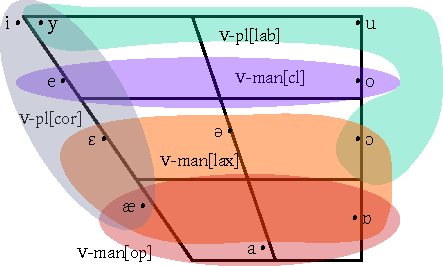
\includegraphics[width=.7\textwidth]{graphics/vowelcharts/bothoa-oral-vowels-features}
  \caption{Featural classes of vowels in in Bothoa Breton}
  \label{fig:natural-classes-bothoa}
\end{figure}


\subsubsection{Stress-related alternations}
\label{sec:stress-relat-altern}

As described above in \cref{sec:stress}, stress mostly stays immobile within a paradigm or across morphologically related items, and where it does move, some form of secondary stress very often remains. Nevertheless, a few alternations can be found.

\paragraph{Data}
\label{sec:data}

As described by \citet{humphreys95:_phonol_bothoa_saint_nicol_pelem}, the plural suffixes \suff{ən} and \suff{jən} cause the stress to shift from a short vowel to the vowel preceding the suffix.\footnote{\citet[p.~247]{humphreys95:_phonol_bothoa_saint_nicol_pelem} says that the stress shift happens \enquote{sometimes}; however, his examples of lack of shift are either words with monosyllabic bases (where the shift applies vacuously) or bases with long vowels, where the shift is blocked for phonological reasons.} These plural suffixes are strongly associated with the agentive derivational suffixes \suff{ər} and \suff{ɛːr}. In the case of the former, the stress shift leads to an alternation between \ipa{[ə]} and \ipa{[æ]}, as shown in \cref{ex:schwa-ae-alternation}:

\ex.\label{ex:schwa-ae-alternation}\a.\a.\twe{[maˈsõːnər]}{masoner}{mason}
\b.\twe{[masoˈnærjən]}{masonerion}{masons}
\z.\b.\a.\twe{[ˈtoːər]}{toer}{roofer}
\b.\twe{[toˈærjən]}{toerion}{roofers}
\b.\mbi{[ˈtoːərjən]}

The alternation between \ipa{[æ]} and \ipa{[ə]} also appears in the conditional suffix \suff{æf} discussed above in \cref{sec:trough-pattern}; the hyphens shows morpheme boundaries for clarity:

\ex.\a.\twe{[ma ˈt-æf-æ]}{ma teufe}{[if] [(s)he] came}
\b.\twe{[ma ˈpaːl-əf-æ]}{ma palfe}{[if] [(s)he] dug}

In general, the vowels \ipa{[æ]}, \ipa{[ɒ]}, and \ipa{[a]} in the \enquote{trough} position all can alternate with the schwa. \Cref{ex:low-vowel-reduction} shows this for \ipa{[ɒ]} and \ipa{[a]}:

\ex.\label{ex:low-vowel-reduction}\a.\a.\twe{[ˈlɒɡɒd̥]}{logod}{mice}
\b.\twe{[ˈlɒɡətad̥]}{logota}{catch mice}
\z.\b.\a.\twe{[ˈtɒhad̥]}{toc'had}{ear (of corn, wheat etc.)}
\b.\twe{[ˈtɒhətad̥]}{toc'hata}{gather, harvest}


However, both these examples involve derivational rather than inflectional morphology. If the trough pattern is created by the addition of inflectional suffixes, the low vowels often remain intact, as seen \cref{ex:bothoa-low-vowel-presevation} with the singulative suffix \suff{ən} and plural \suff{əw}.

\ex.\label{ex:bothoa-low-vowel-presevation}\a.\twe{[ˈlɒɡɒdən]}{logodenn}{mouse}
\b.\twe{[ˈɡɒlɒzəw]}{golvizhier}{beaters}
\b.\twe{[ˈdɒrnəræzəw]}{dornerezhoù}{threshings}

In addition, \ipa{[a]} in the trough position can also be preserved in derivational morphology:

\ex.\label{ex:golched}\a.\twe{[ˈbɒlhad̥]}{golc'hed}{duvet}
\b.\twe{[ˈbɒlhadad̥]}{golc'hedad}{duvet contents}

Note, however, that the suffix \suff{ad} in \cref{ex:golched} is the same suffix that we assumed to be affiliated to the word level with reference to stress data (\cref{sec:strat-aspects-both}), whereas the examples with reduction in \cref{ex:low-vowel-reduction} involve categorial changes, which could reasonably be attributed to the stem level. It would thus appear possible that vowel reduction (at least of \ipa{[a]}) is restricted to the stem level. There are not enough data to provide a confident analysis, however.

It is also possible that the mid vowels \ipa{[ɛ]} and \ipa{[ɔ]} are subject to reduction to schwa in at least some positions. There is evidence for this in the case of \ipa{[ɛ]}. Specifically, both \ipa{[ə]} and \ipa{[ɛ]}, when found in the trough position before a \ipa{[j]} derived from \ipa{[l]} via a palatalization process (see \cref{sec:coron-palat}), undergo coalescence with it to surface as \ipa{[i]}, as seen in \cref{ex:mid-e-reduction}

\ex.\label{ex:mid-e-reduction}\a.\a.\twe{[ˈmɒrzəl]}{morzhol}{hammer}
\b.\twe{[ˈmɒrziəw]}{morzholioù}{hammers}
\z.\b.\a.\twe{[ˈr̥asˌtɛl]}{rastell}{rake}
\b.\twe{[ˈr̥astiəw]}{rastelloù}{rakes}

This is perhaps best analysed as involving reduction from \ipa{[ɛ]} to \ipa{[ə]} in the trough position, unifying the behaviour of the two vowels. In addition, \ipa{[ɛ]} is almost never found in the trough otherwise.\footnote{There is one example, \ipa{[ˈtãnɛrɒh]} `softer' (\emph{teneroc'h}), but it appears anomalous, in that the \ipa{[ɛ]} is the product of an otherwise irregular shortening (\ipa{[tãˈnɛːr]} `tender'), so there is clearly some exceptionality involved.}

In fact, neither \ipa{[ɛ]} nor \ipa{[ɔ]} are very frequent in \enquote{weak} positions, \ie positions other than the main stressed syllable and the final syllable, which, as suggested in \cref{sec:evid-from-segm}, are heads of feet. Neither is found in the trough position. While they may appear in other unstressed syllables, it is overwhelmingly either the initial syllable (which might also be a foot head given \citeauthor{humphreys95:_phonol_bothoa_saint_nicol_pelem}'s description of tertiary stress) or in inflected forms with stress shifts (as in \ipa{[dɛˈvɒtɒh]} `more pious', from \ipa{[ˈdɛvɒd̥]} `pious'), where lack of reduction could be cyclic. Thus, it is not inconceivable that at least \ipa{[ɛ]}, and possibly also \ipa{[ɔ]}, might undergo  reduction to \ipa{[ə]} in some positions, though alternation evidence for \ipa{[ɔ]} is lacking.

\paragraph{Analysis}
\label{sec:analysis}

In terms of the featural specifications shown in \cref{tab:inventory-features-bothoa}, reduction of \ipa{[æ]}, \ipa{[ɒ]}, and \ipa{[ɛ]} (and potentially \ipa{[ɔ]}) can be represented as the delinking of a \fea{V-manner}{open} specification in weak positions. In the case of \ipa{[ɒ]}, this creates \ipa{[ə]} directly; in the case of \ipa{[ɒ]}, the expected segment is \{\fea{V-man}{lax},\fea{V-pl}{cor}\}, \ie the vowel \ipa{[ɛ]}, which is also disallowed in this position and further reduces to \ipa{[ə]}. The relevant autosegmental diagrams are shown in \ref{ex:low-vowel-reduction-autoseg}.

\ex.\label{ex:low-vowel-reduction-autoseg}Reduction of \ipa{[æ]} and \ipa{[ɒ]}\\
\begin{tabular}{l@{\hspace{2em}}l}
  a. Reduction of \ipa{/ɒ/} & b. Reduction of \ipa{/æ/} \\
\begin{tikzpicture}[tree]
\node (rt) {\ipa{ɒ $\rightarrow$ ə}}
  child {node {C-manner}
    child {node (vman) {V-manner}
      child {node (lax) {[lax]}}
      child {node (op) {[open]}}}}
  child {node {C-place}
    child {node {V-place}}};
\join{vman}{op} \delink;
\end{tikzpicture}
&
\begin{tikzpicture}[tree]
\node (rt) {\ipa{æ $\rightarrow$ ə}}
  child {node {C-manner}
    child[narrowtree] {node (vman) {V-manner}
      child {node (lax) {[lax]}}
      child {node (op) {[open]}}}}
  child {node {C-place}
    child {node (vpl) {V-place}
      child {node (cor) {[coronal]}}}} ;
\join{vman}{op} \delink;
\join{vpl}{cor} \delink;
\end{tikzpicture}
\end{tabular}

If the mid vowels \ipa{[ɛ]} and \ipa{[ɔ]} also reduce to schwa in weak positions, both reduction processes can be treated as the delinking of the relevant V-place feature (note that \ipa{[ə]} has a V-place node according to the contrastive hierarchy). This is shown in \ref{ex:mid-vowel-reduction}.

\ex.\label{ex:mid-vowel-reduction}Reduction of \ipa{[ɛ]} and \ipa{[ɔ]}\\
\begin{tikzpicture}[tree]
\node (rt) {\ipa{ɛ/ɔ $\rightarrow$ ə}}
  child {node {C-manner}
    child[narrowtree] {node (vman) {V-manner}
      child {node (lax) {[lax]}}}}
  child {node {C-place}
    child {node (vpl) {V-place}
      child {node (cor) {[coronal]/[labial]}}}} ;
\join{vpl}{cor} \delink;
\end{tikzpicture}

In computational terms, this alternations presents a straightforward instance of the reduction of subsegmental complexity in non-head position, in line with other privative approaches such as those of \citet{harris97:_licen_inher,harris05:_vowel_reduction,harris-urua}. I will assume a positional\hyp faithfulness approach \citep[\egm][]{beckman,alderete1999,iosad10:_motiv}, although nothing in particular hinges on this in Breton. The rankings are shown in \ref{breton-reduction-ranking}. The basic idea is that constraints against complex structures (such as *\us{ə, a, i}, which corresponds to *\ipa{[æ]}, and *\us{ə, a}, \ie *\ipa{[ɒ]}) dominate general \textsc{Max} constraints (which effects vowel reduction) but not \textsc{Max}\hd{} constraints, which block reduction in foot heads.

\ex.\label{breton-reduction-ranking}Vowel reduction in Bothoa Breton\\
\wraptbl{\begin{OTmultitableau}{8}\OTdashes{1,2,4,5,7}\OTsolids{3,6}
\OTmtoprow{\textsc{Max}\hd(\us{i}),\textsc{Max}\hd(\us{a}),\textsc{Max}(\us{ə}),*\us{ə, a, i},*us{ə, i},*\us{ə, a},\textsc{Max}(\us{a}),\textsc{Max}(\us{i})}
\OTmcandrow[/toːær/]{[(ˈtoː)ær]}{,,,*!,*,*,,}
\OTmcandrow{[(ˈtoː)ɛr]}{,,,,*!,,*,}
\OTmcandrow{[(ˈtoː)ɒr]}{,,,,,*!,,*}
\OTmcandrow{[(ˈtoː)ar]}{,,*!,,,,,*}
\OTmcandrow{[(ˈtoː)ir]}{,,*!,,,,*,}
\OTmcandrow[][\OThand]{[(ˈtoː)ər]}{,,,,,,*,*}
\OTmcandrow[/toærjən/][\OThand]{[to(ˈærjən)]}{,,,*,*,*,,}
\OTmcandrow{[to(ˈɛrjən)]}{,*!,,,*,,*,}
\OTmcandrow{[to(ˈɒrjən)]}{*!,,,,,*,,*}
\OTmcandrow{[to(ˈarjən)]}{*!,,*,,,,*,*}
\OTmcandrow{[to(ˈirjən)]}{,*!,*,,,,*,}
\OTmcandrow{[to(ˈərjən)]}{*!,*,,,,*,*}
\end{OTmultitableau}
}

I assume that delinking only affects features rather than nodes, because this allows for an analysis where reduction is driven by constraints on feature co\hyp occurrence (\ie *\ipa{[æ]} and the like), meaning that delinking of entire nodes does not lead to harmonic improvement. An alternative analysis is based on constraints that prohibit the combination of certain features with certain nodes. This would mean that, for instance, the two constraints *\ipa{[ɛ]} (specifically *\{\fea{V-man}{lax}, \fea{V-pl}{cor}\}) and *\ipa{[ɔ]} (*\{\fea{V-man}{lax}, \fea{V-pl}{lab}\}) could be replaced by a single constraint *\{\fea{V-man}{lax}, C-pl\}, which would also (partially) subsume *\ipa{[æ]}. Given the relatively meagre evidence for vowel reduction, any decision at this point is more or less arbitrary. From an architectural perspective, since I recognize both nodes and features as possible arguments in markedness constraints, the difference between the approaches is negligible. I assume the precise choice rides on a closer analysis of the data, whereas conceptually the difference is not enormous.\footnote{In this section I assumed that vowel reduction is in fact a phonological process, possibly with lexical or stratal restrictions. There are some indications that it is not necessarily so and that at least in some cases the vowel written \ipa{[ə]} in the trough position might in fact be a phonological \ipa{[æ]}, meaning that the \phonint{ə} is an artefact of phonetic interpretation \citep[\cfm][]{barnes2007,iosad10:_motiv}. The evidence is provided by the fact that there are some examples of the \ipa{[æ]} in the conditional suffix \suff{æf} surfacing in a medial syllable. One example is \ipa{[ˈøːrəʒæfæ]} `([s]he) would marry'. Note that the \ipa{[æ]} is not in the trough position as defined in \cref{sec:trough-pattern}, although the form does alternate with \ipa{[ˈøːrəʒfæ]}. Another example is \ipa{[ˌkusˈkæfæ]} `([s]he) would sleep', which coexists with \ipa{[ˈkuskfæ]}, and note the irregular stress pattern. Both examples are noted for one speaker, and are described as \enquote{sporadic variants} (\foreigntextquote{french}{avec le statut de variantes sporadiques}). The issue can only be resolved by empirical study.}

\subsubsection{Vowel raising}
\label{sec:vowel-raising}

Short unstressed \ipa{[e]} productively alternates with \ipa{[i]} in hiatus (recall that phonetically this \ipa{[i]} may be realized as a non-syllabic glide). This \ipa{[i]} can be preceded by dorsal stops.

\ex.\a.\a.\twe{[ˈalve]}{alc'hwez}{key}
\b.\twe{[ˈalviəw]}{alc'hwezioù}{keys}
\b.\mbp{ˈalvjəw}
\z.\b.\a.\twe{[ˈklɔːɡe]}{kloge}{ladle}
\b.\twe{[ˈklɔːɡiəw]}{klogeoù}{ladles}
\b.\mbp{ˈklɔːɡjəw}
\z.\b.\a.\twe{[ˈʃaːre]}{charre}{scythe handle}
\b.\twe{[ˈʃaːriad̥]}{charread}{forceful blow}
\z.\b.\a.\twe{[ˈbøːre]}{beure}{morning}
\b.\twe{[ˈbøːriɒh]}{beureoc'h}{earlier in the morning}


However the raising is motivated (note that in all cases it happens in the trough position, since an unstressed \ipa{[e]} is in these cases preceded by a stressed syllable and necessarily followed by another syllable), in autosegmental terms it is easily understood as the delinking of a \fea{V-manner}{closed} feature, as seen in \cref{ex:e-raising}.

\ex.\label{ex:e-raising}Raising of \ipa{[e]} via delinking\\
\begin{tikzpicture}[tree]
\node (rt) {\ipa{e $\rightarrow$ i}}
  child {node {C-manner}
    child {node (vman) {V-manner}
      child {node (cl) {[closed]}}}}
  child {node {C-place}
    child {node {V-place}
      child {node {[coronal]}}}} ;
\join{vman}{cl} \delink;
\end{tikzpicture}

Again, in principle this process might be treated as delinking of the manner node rather than of the feature, but this would require a more complicated analysis which would have to account for the lack of similar alternations with \ipa{[o]}. There are indeed no examples of \ipa{[o]} raising to \ipa{[u]} in a similar context, which might be explained by the fact the deleting the manner specification from \ipa{[o]} would result in an otherwise prohibited empty segment. However, any account of the behaviour of \ipa{[o]} would be pure conjecture: there is only one example of \ipa{[o]} in hiatus (\ipa{[toˈærjən]} `roofers'), but \ipa{[o]} is not in the trough position, and in addition it coexists with \ipa{[ˈtoːərjən]}, which makes the status of the form less clear. Thus, for the sake of the argument I will assume that raising is explained by some constraint prohibiting \{\fea{V-man}{cl}, \fea{V-pl}{cor}\} in hiatus dominating \textsc{Max}(\fea{V-man}{cl}) but not \textsc{Max}(\fea{V-pl}{cor}).

\subsubsection{The nasal vowels}
\label{sec:nasal-vowels-1}

I do not discuss the nasal vowels at length in this dissertation. I note two particular properties that would need to be discussed in a fuller account of Bothoa Breton phonology.

\paragraph{Representational issues}
\label{sec:repr-issu}

There is suggestive evidence for treating nasal vowels as representationally related to the coronal nasal \ipa{[n]}. The clearest evidence is provided by alternations such as that shown in \cref{ex:pontiou}

\ex.\label{ex:pontiou}\a.\twe{[ˈpond̥]}{pont}{bridge}
\b.\twe{[ˈpõːʃəw]}{pontioù}{bridges}

Here, the nasal does not appear because of a restriction on homorganic nasal\endash fricative sequences which appears to be exceptionless in Bothoa Breton.\footnote{Non-homorganic sequences are allowed: \ipa{[ˈamzər]} `weather', \ipa{[ˈpinviʧad̥]} `enrich oneself'.} Instead, the nasal coalesces with the preceding vowel. A contrast between \ipa{[Ṽn]} and \ipa{[Vn]} sequences seems to exist, but it is said to be most robust in unstressed position, and it is not immediately clear that unstressed \enquote{nasal vowels} are not really the result of a gesture overlap under conditions of reduced duration. No definitive pronouncements appear possible at this stage.

\paragraph{Length}
\label{sec:length}

According to \citet{humphreys95:_phonol_bothoa_saint_nicol_pelem}, length is not distinctive for nasal vowels in Bothoa Breton except \ipa{[ã]} in the position before \ipa{[n]} (which is also interesting in view of the relationship between nasal vowels and \ipa{[n]} just sketched). This conclusion is based on the rôle of the nasal vowels in lexical contrast, which is indeed restricted. However, nasal vowels do appear to obey restrictions on long vowels, in that unstressed nasal vowels (which, except \ipa{[ã]}, are relatively infrequent) are uniformly short. Since prosody is not necessarily lexically contrastive, the length of nasal vowels might need to be represented in the phonology somehow. Again, I leave this matter aside here.

\subsubsection{Diphthongs}
\label{sec:diphthongs-bothoa}

As discussed in \cref{sec:diphthongs}, the diphthongs of Bothoa Breton are \ipa{[ɛĭ]}, \ipa{[əy̆]}, \ipa{[əw]} and \ipa{[aw]}, and \ipa{[ãw̃]}. Phonologically, their most important characteristic is that they pattern with short rather than long vowels in that they do no necessarily attract stress and that they may precede tautosyllabic consonants.

In \cref{sec:syll-size-restr} I have argued that diphthongs are best represented as a single branching mora. Further, I propose that the mora dominates segments which from a featural perspective are both vowels, just as in Welsh.

The non-nucleus part of the diphthong can only contain mannerless segments (\ie the high vowels). While this is not necessarily significant in view of the typological frequency of such a pattern, it might also be taken as additional evidence for the status of high vowels as mannerless segments, as this restriction receives a straightforward featural basis: no V-manner nodes are allowed in the non-head portion of a diphthong.

As for the nuclear portion, there is evidence for just one contrast in nucleus quality: that of \ipa{[əw]} (which is \phonint{æw} for some speakers) versus \ipa{[aw]}. I suggest that from a phonological perspective the possible diphthongal nuclei are \ipa{[ə]} (\fea{V-manner}{lax}) and \ipa{[a]} (\fea{V-manner}{open}), with no V-place features, or more generally complex segments, allowed in diphthong nuclei.\footnote{The apparent lack of diphthongs with a \ipa{[o]} nucleus has to be admitted as a lexical gap.} If this generalization is correct, it provides some evidence for \ipa{[ə]} and \ipa{[a]} as unit segments for V-manner features. Thus, in the remainder of this chapter I will use the phonological notation for diphthongs as shown in \cref{tab:diphthong-notation-breton}. I use the symbol \ipa{[w]} rather than \ipa{[u]} for the diphthongal glide for consistency with \ipa{[ãw̃]}.

\begin{table}[htp]
  \centering
  \begin{tabular}{*{2}{l}}
    \toprule
    Phonetic notation & Surface phonology \\
    \midrule
    \ipa{[ɛĭ]} & \ipa{[əi]} \\
    \ipa{[əy̆]} & \ipa{[əy]} \\
    \ipa{[əŭ]/[æŭ]} & \ipa{[əw]} \\
    \midrule
    \ipa{[aŭ]} & \ipa{[aw]} \\
    \ipa{[ãŭ̃]} & \ipa{[ãw̃]} \\
    \bottomrule
  \end{tabular}
  \caption{Phonological notation for diphthongs}
  \label{tab:diphthong-notation-breton}
\end{table}


\subsubsection{Morphologically conditioned alternations}
\label{sec:morph-cond-altern}

A number of vowel changes in inflection appear to be driven by morphology or even triggered on a word-by-word basis.

The back vowels \ipa{[a]}, \ipa{[ɔ]} and \ipa{[ã]} are fronted to \ipa{[i]} by the plural suffix \suff{i}, but this suffix is unproductive and extremely rare. Instances for \ipa{[i]} that appear in this formation trigger palatalization of dorsal stops to postalveolar fricatives.

\ex.\a.\a.\twe{[ˈkɔɡ̊]}{kog}{rooster}
\b.\twe{[ˈʧiːdʒi]}{kegi}{roosters}
\z.\b.\a.\twe{[ˈpɔːləz̥]}{polez}{chicken}
\b.\twe{[ˈpiləzi]}{polezi}{chickens}
\z.\b.\a.\twe{[ˈɡast]}{gast}{bitch}
\b.\twe{[ˈdʒisti]}{gisti}{bitches}
\z.\b.\a.\twe{[ˈbrãːn]}{bran}{crow}
\b.\twe{[ˈbriːni]}{brini}{crows}

There is a very small class of nouns forming plurals purely by vowel change, such as \ipa{[ˈmiːn]} `stone' (\emph{maen}), plural \ipa{[ˈməin]} (\emph{mein}); I do not have much to say about these alternations here.

\subsubsection{Summary: vowels}
\label{sec:summary:-vowels}

Despite having a relatively large vowel inventory, Bothoa Breton does not exhibit many vocalic alternations that would give evidence for the representations. The alternation classes I propose for Bothoa Breton are shown in \cref{fig:alt-classes-bothoa}. In addition to the classes discussed in this section, \ipa{[i]} and \ipa{[y]} are grouped together because they trigger a palatalization process, as described below in \cref{sec:palatalization}.
\begin{figure}[htp]
  \centering
  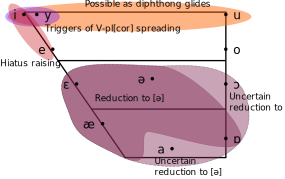
\includegraphics[width=.7\textwidth]{graphics/vowelcharts/bothoa-oral-vowels-classes}
  \caption{Alternation classes in Bothoa Breton}
  \label{fig:alt-classes-bothoa}
\end{figure}


As \cref{fig:alt-classes-bothoa} shows, the evidence for some of the specifications I propose is rather inconclusive; in some cases, as in the case of \ipa{[o]}, the assignment of features has to be relatively arbitrary. However, this system allows us to give an account of such facts as can be gleaned from \posscite[']{humphreys95:_phonol_bothoa_saint_nicol_pelem} description. A fuller account is of course possible, but it requires a better understanding of the possible alternations and their conditioning, as well as of the interaction between prosody and segmental phonology, than is available at the moment

\subsection{Consonant representations and alternations}
\label{sec:cons-altern}


The featural specifications I propose for consonants are given in \cref{tab:bothoa-consonant-features}. To save space, \cref{tab:bothoa-consonant-features} only gives \emph{featural} specifications, whereas empty nodes whose appearance is driven by contrastive specification are discussed in more detail below.

\begin{table}[htp]
  \centering
\resizebox{\textwidth}{!}{
  \begin{tabular}{lccccccccc}
    \toprule
& \multicolumn{2}{c}{C-place} & \multicolumn{2}{c}{V-place} & \multicolumn{2}{c}{C-manner} & \multicolumn{2}{c}{V-manner} & C-laryngeal \\
\cmidrule(r){2-3}
\cmidrule(lr){4-5}
\cmidrule(lr){6-7}\cmidrule(lr){8-9}\cmidrule(l){10-10}
Segment    & [labial]      & [coronal]     & [coronal]     & [labial]      & [open]        & [closed]      & [open]        & [closed]      & [voiceless]   \\
\midrule
\ipa{/p/}  & \checkmark    &               &               &               &               & \checkmark    &               &               & \checkmark    \\
\ipa{/b/}  & \checkmark    &               &               &               &               & \checkmark    &               &               &               \\
\ipa{/t/}  &               & \checkmark    &               &               &               & \checkmark    &               &               & \checkmark    \\
\ipa{/d/}  &               & \checkmark    &               &               &               & \checkmark    &               &               &               \\
\ipa{/k/}  &               &               &               &               &               & \checkmark    &               &               & \checkmark    \\
\ipa{/ɡ/}  &               &               &               &               &               & \checkmark\gc &               &               &               \\
\ipa{/ɡw/} &               &               &               & \checkmark    &               & \checkmark    &               &               &               \\
\midrule
\ipa{/ʧ/}  &               &               & \checkmark    &               &               & \checkmark    &               &               & \checkmark    \\
\ipa{/dʒ/} &               &               & \checkmark    &               &               & \checkmark    &               &               &               \\
\ipa{/dʒɥ/}& \checkmark    &               & \checkmark    &               &               & \checkmark    &               &               &               \\
\midrule
\ipa{/f/}  & \checkmark    &               &               &               &               &               &               &               & \checkmark    \\
\ipa{/v/}  & \checkmark\gc &               &               &               &               &               &               &               &               \\
\ipa{/s/}  &               & \checkmark    &               &               &               &               &               &               & \checkmark    \\
\ipa{/z/}  &               & \checkmark\gc &               &               &               &               &               &               &               \\
\ipa{/ʃ/}  &               & \checkmark    & \checkmark    &               &               &               &               &               & \checkmark    \\
\ipa{/ʒ/}  &               & \checkmark    & \checkmark    &               &               &               &               &               &               \\
\ipa{/h/}  &               &               &               &               &               &               &               &               & \checkmark\gc \\
\midrule
\ipa{/ɥ/}  & \checkmark    &               & \checkmark    &               &               &               &               &               &               \\
\midrule
\ipa{/n/}  &               &               &               &               & \checkmark    &               &               & \checkmark    &               \\
\ipa{/m/}  & \checkmark    &               &               &               & \checkmark    &               &               & \checkmark    &               \\
\ipa{/j̃/}  &               &               & \checkmark    &               & \checkmark    &               &               & \checkmark    &               \\
\ipa{/l/}  &               &               &               &               & \checkmark\gc &               &               &               &               \\
\ipa{/r/}  &               &               &               &               & \checkmark    &               & \checkmark    &               &               \\
\midrule
\ipa{/i/}  &               &               & \checkmark\gc &               &               &               &               &               &               \\
\ipa{/a/}  &               &               &               &               &               &               & \checkmark\gc &               &               \\
\ipa{/o/}  &               &               &               &               &               &               &               & \checkmark\gc &               \\
\ipa{/u/}  &               &               &               & \checkmark\gc &               &               &               &               &               \\
\bottomrule
  \end{tabular}}
  \caption{Featural specifications for consonants in Bothoa Breton}
  \label{tab:bothoa-consonant-features}
\end{table}

Note that, as in the case of Welsh, I associate contrastive non-specification for a feature with the presence of a bare featural node. An important feature of Bothoa Breton, as I argue below, is that it makes use of the possibility of ternary contrasts (presence of a feature \vs presence of a bare node \vs absence of a feature) in surface phonological representations.

In this section I consider palatalization, high vowel gliding, and word-level laryngeal phonology, before moving on to initial mutations.

\subsubsection{Palatalization}
\label{sec:palatalization}

I discuss two kind of palatalization separately: the palatalization of dorsals by high front vowels and the palatalization of coronals and dorsals due to coalescence with an onset \ipa{[i]}.

\paragraph{Velar palatalization}
\label{sec:velar-palatalization}

The postalveolar affricates \ipa{[ʧ]} and \ipa{[dʒ]} appear in many contexts where there is no evidence for deriving them from other segments: they contrast with dorsal stops, fail to alternate with them, and the context is not \emph{a priori} conducive to palatalization. This is shown in \cref{ex:postalveolar-contrasts}.

\ex.\label{ex:postalveolar-contrasts}\a.\a.\twe{[ˈsʧøːl]}{skeul}{ladder}
\b.\twe{[ˈkəwəd̥]}{kavout}{find}
\z.\b.\a.\twe{[ˈʧɛvələɡ̊]}{kefeleg}{woodcock}
\b.\twe{[kazəˈkɛnəɡ̊]}{kazekenned}{mares}
\z.\b.\a.\twe{[ˈʧahəd̥]}{kerzhet}{to walk}
\b.\twe{[ˈkaləd̥]}{kalet}{hard}

This would seem to demonstrate that \ipa{[ʧ]} and \ipa{[dʒ]} are part of the inventory of underlying segments. I suggest this is indeed the case. Nevertheless, there is also evidence that at least some instances of \ipa{[ʧ]} and \ipa{[dʒ]} are derived from dorsal stops.

\subparagraph{Data}
\label{sec:data-1}

First, sequences of dorsal stops \ipa{[k~ɡ]} (phonetically \phonint{kʲ~ɡʲ} in this position) followed by high front vowels \ipa{[i~y]} are relatively rare in the language. The sequence \ipa{[ky]} appears not to be found at all, while \ipa{[ɡy]} is only attested in the clearly borrowed name \ipa{[ɔɡysˈtiːn]} `Augustine' (in addition, it is found in an underived form, which are known to sustain exceptions). As for \ipa{[ki]} and \ipa{[ɡi]}, they are found in the following contexts:

\begin{itemize*}
\item Postlexically:
\end{itemize*}

\ex.\a.\twe{[ak i ˈziː]}{hag he zi}{and her house}
\b.\twe{[aɡ ˈivul]}{hag eoul}{and oil}

\begin{itemize*}
\item Before the future suffixes \suff{id̥} (2nd person plural), \suff{iːãmp} (1st person plural), \suff{iːaj̃\kern-1pt ʧ} (2rd person plural):
\end{itemize*}

\ex.\a.\twe{[ˈlakiãmb̥]}{lakiamp}{we will put}
\b.\twe{[ˈpleːɡid̥]}{plegit}{you (pl.) will fold}

\begin{itemize*}
  \item Before certain derivational suffixes:\footnote{There are also exists a derivational suffix \suff{yz̥}, but there appear to be no relevant examples.}
\end{itemize*}

\ex.\a.\twe{[ˈvrãŋkiz̥]}{frankiz}{open space, the outdoors}
\b.\twe{[ˈbeɡiʃad̥]}{begisat}{to chatter}

\begin{itemize*}
  \item Before instances of \ipa{[i]} derived by raising (\cref{sec:vowel-raising}):
\end{itemize*}

\ex.\a.[]\twe{[ˈklɒːɡiəw]}{klogeoù}{ladles}


Alternations between dorsal stops as such and the affricates are few and far between. They are found with the plural suffix \suff{i}, which also causes the otherwise irregular overwriting of the root vowel with an \ipa{[i(ː)]}. This high vowel in the root also causes the alternation.\footnote{There is also at least one instance of velar palatalization in an irregular plural before a non-high front vowel: \ipa{[dʒɛvər]} `goats' (\emph{gevr}), \cf singular \ipa{[ˈɡawr]}.}

\ex.\a.\a.\twe{[ˈkɔɡ̊]}{kog}{rooster}
\b.\twe{[ˈʧiːdʒi]}{kegi}{roosters}
\z.\b.\a.\twe{[ˈɡast]}{gast}{bitch}
\b.\twe{[ˈdʒisti]}{gisti}{bitches}

I suggest that the fact that \ipa{[k]} and \ipa{[ɡ]} are all but excluded from the position before high front vowels morpheme-internally indicates that the phonological computation maps the dorsal stops to \ipa{[ʧ]} and \ipa{[dʒ]} in this context. I will refer to this alternation as velar palatalization. It happens only at the stem level, explaining the paucity of alternations, as well as the fact that the alternation is blocked before \ipa{[i]} derived by raising; in \cref{sec:gliding} below I argue that raising is a word-level process, which explains the counterfeeding relationship. It is noteworthy that clearly inflectional suffixes such as the future morphemes do not trigger velar palatalization, since inflection is normally assumed to happen only at the word level.\footnote{\label{fn:kegi-stratal}Note, however, that the inflectional suffix \suff{i} also appears to trigger this alternation in \ipa{[ˈʧiːdʒi]} `roosters', from \ipa{[ˈkɔɡ̊]}. Following \citet{bermudez-oterong}, I suggest that this form is an irregular root-based formation rather than one where the inflectional suffix is added to the stem, as demonstrated by the fact that the root allomorph \ipa{[ˈʧiːdʒ]} is bound, and root\hyp based formations undergo stem\hyp level phonology. See also below \cref{sec:front-unro-vowel} for more discussion.}

Moreover, at least in the case of \ipa{[ʧ]} there is evidence from initial consonant mutations that some tokens of word-initial affricates are derived from underlying dorsal stops followed by \ipa{[j]}. Specifically, the so-called spirantization (see below \cref{sec:spirantization}) involves a change from \ipa{[k]} to \ipa{[h]}. Moreover, when the \ipa{[k]} precedes a sonorant, the result is the so-called voiceless sonorant (as discussed below in \cref{sec:spirantization}, this is important evidence for representing voiceless sonorants as \ipa{[h]}\endash sonorant sequences). This is shown in \cref{ex:k-spirantization}.

\ex.\label{ex:k-spirantization}\a.\a.\twe{[ˈkaːz̥]}{kazh}{cat}
\b.\twe{[mə ˈhaːz̥]}{ma c'hazh}{my cat}
\z.\b.\a.\twe{[ˈkriːb̥]}{krib}{comb}
\b.\twe{[mə ˈhriːb̥]}{ma c'hrib}{my comb}

The outcome of the spirantization of \ipa{[ʧ]} in the sequence \ipa{[ʧɥ]} is the same as that of \ipa{[k]} before sonorants

\ex.\a.\twe{[ˈʧɥiːzin]}{kegin}{kitchen}
\b.\twe{[i hɥiːzin]}{he c'hegin}{her kitchen}


This behaviour is consistent with the word for `kitchen' being underlyingly represented as \ipa{/kɥiːzin/}.

Similarly, \ipa{[ʧ]} before a high front vowel is spirantized to \ipa{[h]}, which could potentially be derived if the \ipa{[ʧ]} corresponded to \ipa{/k/}:

\ex.\a.\twe{[ˈʧiː]}{ki}{dog}
\b.\twe{[ə ˈhiː]}{ar c'hi}{the dog}

No such argument from mutation can be made for \ipa{[dʒ]}. If words such as \ipa{[dʒiːr]} `word' (\emph{ger}) had an underlying dorsal stop, we would expect that stop to become \ipa{[h]} in the course of lenition (\cref{sec:lenition}). However, this does not happen, and \ipa{[dʒ]} remains unchanged:

\ex.\label{ex:no-dz-as-g}\a.\a.\twe{[ˈɡɔˌdɛl]}{godell}{pocket}
\b.\twe{[i ˈhɔˌdɛl]}{e c'hodell}{his pocket}
\z.\b.\a.\twe{[ˈdʒiːr]}{ger}{word}
\b.\twe{[i ˈdʒiːr]}{e c'her}{his word}
\b.*\mbi{[i ˈhiːr]}

There is thus very little evidence for underlying \ipa{/ɡi/} sequences which surface as \ipa{[dʒi]}, even though there is circumstantial evidence for a \ipa{/ɡ/}$\rightarrow$\ipa{/dʒ/} change before high front vowels in forms such as \ipa{[ˈdʒisti]} (as the plural of \ipa{[ˈɡast]}).\footnote{\label{fn:article-allomorphy}\citet{humphreys95:_phonol_bothoa_saint_nicol_pelem} discusses another type of evidence for a distinction between underived \ipa{[ʧ~dʒ]} and derived ones. Briefly, Bothoa Breton distinguishes between two allomorphs of the definite and indefinite articles, which are sensitive to the phonology of the following word. Of particular interest here is the distinction between following coronals and non-coronals: \ipa{[ən ˈdɒrz̥]} `the bread roll' (\emph{an dorzh}) but \ipa{[ə ˈɡəw]} `the lie' (\emph{ar gaou}). In the case of \ipa{[ʧ]} and \ipa{[dʒ]}, the article allomorphy reproduces the diachronic origin: \ipa{[n]}-ful forms are chosen before affricates descending from *\emph{tj} and *\emph{dj} (\ipa{[ən ˈdʒəwl]} `the devil', \cf Welsh \emph{diawl}) but \ipa{[n]}-less forms are used before those going back to dorsals (\ipa{[ə ˈdʒiːr]} `the word', \cf Welsh \emph{gair}). Similarly, underlying initial \ipa{[h]} is associated with \ipa{[n]}-ful forms (\ipa{[ən ˈhãw̃n]} `the name') but \ipa{[h]} derived from \ipa{[ʧ]} (and ultimately \ipa{[k]}) takes \ipa{[n]}-less forms like dorsals (\ipa{[ə ˈhiː]} `the dog', \cf Welsh \emph{cî}). However, I suggest that the article allomorphy cannot be used to diagnose the phonological make-up of following words. First, it is also sensitive to etymological differences that are not recoverable from synchronic alternations, as in the case of initial \ipa{[hw]} (\ipa{[n]}-ful forms before \emph{*huV} and \ipa{[n]}-less forms before *\emph{\ipa{χw}}), so at least some arbitrary subcategorization must be involved (note that I assume \ipa{[w]} and \ipa{[u]} are not phonologically distinct in Bothoa Breton). Second, the class of onsets selecting for \ipa{[n]}-ful forms (\ipa{[t~d~$\emptyset$~h~w]}) does not seem to be motivated by the featural structure of the language otherwise. Finally, if the selection of the article allomorphs were driven by the phonology, it would have to be sensitive to the featural make-up of the initial consonant \emph{before} the application of the palatalization rule. However, palatalization is a stem-level rule, whereas the article is clearly a separate lexical item: this creates an ordering paradox, since one would expect insertion of the article to follow the entire cycle of the phonological derivation in the noun. While this may appear less of an issue in fully parallel frameworks, one would still have to deploy whatever machinery one uses to deal with counterbleeding opacity in this case. Moreover, this example demonstrates the greater restrictiveness of stratal models: while fully parallel frameworks and some current versions of serial OT allow the interaction of any two processes (\eg via \textsc{Prec} constraints in the case of the latter), stratal models impose more restrictive global conditions on rule ordering (\citealp[\cf][]{kiparsky11:_chain} on this point), and they predict such an interaction to be impossible.} I conclude that a process of velar palatalization is active at the stem level in Bothoa Breton, producing \ipa{[ʧ]} and \ipa{[dʒ]} from \ipa{[k]} and \ipa{[ɡ]} before \ipa{[i~y]} (the absence of the opaque mutation pattern of \cref{ex:no-dz-as-g} is accounted for in \cref{sec:lexic-insert-strat}).

\subparagraph{Analysis}
\label{sec:analysis-1}

In featural terms, velar palatalization is represented as a straightforward process of the spreading of \fea{V-pl}{coronal} from \ipa{[i]} and \ipa{[y]} to the placeless dorsal stops. This is shown in \cref{ex:velar-analysis}.

\ex.\label{ex:velar-analysis}Velar palatalization: \ipa{/ki/} $\rightarrow$ \ipa{[ʧi]}\\
\begin{tikzpicture}[tree]
  \node (k) {\ipa{k $\rightarrow$ ʧ}}
  child {node {C-manner}
    child {node {[closed]}}}
  child {node {C-laryngeal}
    child {node {[voiceless]}}} ;
  \node[right=8em of k] (i) {\ipa{i}}
  child {node (cpl) {C-place}
    child {node {V-place}
      child {node {[coronal]}}}} ;
  \join[draw,dashed]{k}{cpl} ;
\end{tikzpicture}


The process of velar palatalization thus provides evidence both for the featural specification of \ipa{[i]} and \ipa{[y]} as \fea{V-place}{coronal} vowels and the markedness relationships and place specifications for the nonanterior stops. Such relationships, with dorsals unmarked for place and easily susceptible to place changes, are of course not uncommon, as documented by \citet[\eg][]{rice96:_defaul_variab,rice03:_featur}.

There are two further remarks that must be made here. First, I assume that spreading is triggered only by \ipa{[i]} and \ipa{[y]} that are parsed as nuclei; see the next section for discussion of onset \ipa{[i]} and \ipa{[y]}. Second, note that spreading is triggered only by those \fea{V-place}{coronal} vowels that do not bear any V-manner features. I suggest that both these restrictions can be expressed as restrictions on domain heads \citep{kenstowicz1997,moren01:_distin,delacy2002,lacy04:_marked_optim_theor,delacy2006,jurgec10:_featur_spread}.

In OT terms, this requires that some constraint driving spreading dominate \textsc{DepLink}(\fea{V-pl}{cor}), although it is dominated by constraints on domain heads. In this instance, we require the following constraints, using the notation \dtei{F} to mean \enquote{head (or \enquote{designated terminal element}) of the domain of [F]} (Following \citealt{jurgec10:_featur_spread}, I assume that \dte-constraints only apply to heads of branching domains, \ie that they are not the same as feature co-occurrence restrictions or moraic enhancement constraints.)

\ex.*\dtei{\fea{V-pl}{cor}}\fea{V-man}{lax}/[cl]: \enquote{assign a violation mark for each head of a \fea{V-pl}{cor} domain that also bears a \fea{V-man}{lax}/\fea{V-man}{cl} feature}.\footnote{It is not enough to ban the presence of a V-manner node with the feature set proposed in \cref{fig:bothoa-contrastive-hierarchy}, because \ipa{[i]} and/or \ipa{[y]} always have to be specified for V-manner to distinguish them from other \fea{V-pl}{cor} segments.}

\ex.\textsc{Have}-\mo/\dtei{\fea{V-pl}{cor}}: \enquote{assign a violation mark for each head of a branching \fea{V-pl}{cor} domain that does not also head a moraic domain}. This constraint ensures that spreading of \fea{V-pl}{cor} only happens from nuclear positions.

As in \cref{cha:pembrokeshire-welsh}, I use the non-committal constraint schema \textsc{Share} to drive spreading. The ranking is shown in \ref{ki-kezek-kloge}, using \ipa{[ˈʧiː]} `dog' to demonstrate palatalization and \ipa{[ˈklɒːɡe]} `ladle' to show lack of spreading from complex segments. I also show the result for an underlying \ipa{/kiɛzeɡ/} `horses', where, under the ranking given in \cref{ki-kezek-kloge}, palatalization fails because the high front vowel is parsed as an onset, so the output at the stem level is \ipa{[kjɛzəɡ]}. This form ultimately surfaces as \ipa{[ˈʧɛzəɡ̊]}, as discussed in \cref{sec:coron-palat} and \cref{sec:gliding}.  To save space, I do not show the constraint \textsc{Max}(\fea{V-man}{cl}) which ensures that this feature is not deleted to satisfy *\dtei{\us{i}}/\fea{V-man}{lax}, as in \ipa{[ˈklɒːdʒi]} for \ipa{/klɒːɡe/}. More nuanced description of the constraint \textsc{Uniformity} also follows below (\cpageref{sec:stem-level} \emph{sqq.}).

\ex.\label{ki-kezek-kloge}Velar palatalization\\
\wraptbl{\begin{OTmultitableau}{7}\OTdashes{1,2,3,6}\OTsolids{4,5}
\OTmtoprow{\textsc{Uniformity},\textsc{Have}-\mo/\dtei{\us{i}},*\dtei{\us{i}}\us{o, ə},\textsc{Onset},\textsc{Share}(\us{i}),\textsc{DepLink}(\us{i}),\textsc{*ComplexOnset}}
\OTmcandrow[/ki/]{[k\fd{iː\smo\smo}{i}]}{,,,,*!,,}
\OTmcandrow[][\OThand]{[\fd{ʧiː\smo\smo}{i}]}{,,,,,*,}
\OTmcandrow[/klɒːɡe/][\OThand]{[ˈklɒːɡ\fd{e\smo}{i}]}{,,,,*,,}
\OTmcandrow{[ˈklɒː\fd{dʒe\smo}{i}]}{,,*!,,,*,}
\OTmcandrow[/kiɛzəɡ/]{[k\fd{i\smo}{i}.ɛ\smo{}zəɡ]}{,,,*!,*,,}
\OTmcandrow{[\fd{ʧi\smo}{i}.ɛ\smo{}zəɡ]}{,,,*!,,*,}
\OTmcandrow[][\OThand]{[k\fd{j}{i}ɛ\smo{}zəɡ]}{,,,,*,,*}
\OTmcandrow{[\fd{ʧj}{i}ɛ\smo{}zəɡ]}{,*!,,,,*,*}
\OTmcandrow{[\fd{ʧ}{i}ɛ\smo{}zəɡ]}{*!,,,,,,}
\end{OTmultitableau}
}

\paragraph{Coronal palatalization}
\label{sec:coron-palat}

The process that I call coronal palatalization, or \enquote{coalescence}, is triggered by certain suffixes.

\subparagraph{Data}
\label{sec:data-7}

In the case of coronal obstruents, coalescence produces postalveolar fricatives \ipa{[ʃ]} and \ipa{[ʒ]}, except in the case of the sequence \ipa{[st]}, in which case the outcome is \ipa{[sʧ]}. The following examples show the alternations:

\ex.\ipa{[d]} $\rightarrow$ \ipa{[ʒ]}
\a.\a.\twe{[ˈpraːd̥]}{prad}{prayer}
\b.\twe{[ˈpraːʒəw]}{pradoù}{prayers}
\z.\b.\a.\twe{[ˈøːrəd̥]}{eured}{marriage}
\b.\twe{[ˈəːrəʒo]}{eurediñ}{marry}

\ex.\ipa{[t]} $\rightarrow$ \ipa{ʃ}
\a.\a.[]\twe{[ˈpond̥]}{pont}{bridge}
\z.\b.\a.[]\twe{[ˈpõːʃəw]}{pontioù}{bridges}

\ex.\ipa{/z/} $\rightarrow$ \ipa{[ʒ]}
\a.\a.\twe{[ˈmiːz̥]}{miz}{month}
\b.\twe{[ˈmiːʒəw]}{mizioù}{months}
\z.\b.\a.\twe{[ˈtemz̥]}{temz}{manure}
\b.\twe{[ˈtemʒo]}{temzañ}{fertilize with manure}

\ex.\ipa{[s]} $\rightarrow$ \ipa{[ʃ]}
\a.\a.[]\twe{[ˈplaz̥]}{plas}{place}
\z.\b.\a.[]\twe{[ˈplaʃəw]}{plasoù}{places}

\ex.\ipa{[st]} $\rightarrow$ \ipa{[sʧ]}
\a.\a.[]\twe{[ˈlɒst]}{lost}{tail}
\b.[]\label{lostou}\twe{[ˈlɒsʧəw]}{lostoù}{tails}

\ex.\ipa{[n]} $\rightarrow$ \ipa{/j̃\kern-1pt/} (phonetically \phonint{ɲ} or \phonint{j̃\kern-1pt})
\a.\a.\twe{[ˈpwiːn]}{poan}{pain}
\b.\twp{ˈpwiːj̃\kern-1pt əw}{poanioù}{pains}
\z.\b.\a.\twe{[ˈʧærn]}{korn}{horn}
\b.\twp{ˈʧærɲəw}{kornioù}{horns}

\ex.\ipa{[l]} $\rightarrow$ \ipa{[j]}
\a.\a.[]\twe{[ˈpaːl]}{pal}{shovel}
\z.\b.\a.[]\twe{[ˈpaːjəw]}{palioù}{shovels}

\ex.\ipa{[ˌɛl]}, \ipa{[əl]} $\rightarrow$ \ipa{[i]}
\a.\a.[]\twe{[ˈmɒrˌzɛl]}{morzhol}{hammer}
\z.\b.\a.[]\twe{[ˈmɒrziəw]}{morzholioù}{hammers}


I interpret this phenomenon as involving coalescence with an onset \ipa{[i]}. That at least some relevant suffixes do contain this segment in their segmental representations is demonstrated by the examples in \ref{ex:broiou-feurmiou}

\ex.\label{ex:broiou-feurmiou}The plural suffixes \suff{iəw} and \suff{iən}
\a.\a.\twe{[ˈbroː]}{bro}{country}
\b.\twe{[ˈbrojəw]}{broioù}{countries}
\z.\b.\a.\twe{[ˈlɛvər]}{levr}{book}
\b.\twe{[ˈlɛvərjəw]}{levrioù}{books}
\z.\b.\a.\twe{[ˈɛskɔb̥]}{eskob}{bishop}
\b.\twe{[ɛsˈkɔbjən]}{eskibien}{bishops}

\ex.\label{ex:otoiad-keriad}The derivational suffix \suff{iad}
\a.\a.\twe{[ɔˈtɔː]}{oto}{car}
\b.\twe{[ɔˈtɔjad̥]}{otoiad}{contents of a car}
\z.\b.\a.\twe{[ˈlwɛːr]}{loar}{moon}
\b.\twe{[ˈlwɛːrjad̥]}{loariad}{lunar month}

Importantly, the explicit \ipa{[j]} appears following exactly those segments that do not undergo coronal palatalization, \ie vowels, labials, and \ipa{[r]}.

As for dorsals before onset \ipa{[i]}, the evidence is somewhat ambiguous. Historically, *\emph{kj} tended to give \emph{ʃ} and *\emph{gj} could yield either \emph{ʒ} or \emph{j} \citep[§585]{histbreton}. In the case of \emph{kj~gj}\,$\rightarrow$\,\emph{ʃ~ʒ}, the treatment is identical to that of coronal stops, although not in the case of *\emph{gj}\,$\rightarrow$\emph{j}.

Examples with suffixation are not abundant, but it is at least possible for sequences of a dorsal stop and \ipa{[j]} to coalesce into affricates:

\ex.\label{elastique}\a.\twe{[ˌlasˈtikən]}{}{rubber band (French \emph{\textfrench{élastique}})}
\b.\twe{[ˈlastiʧəw]}{}{rubber bands}

There is also some evidence for palatalization\hyp as\hyp spirantization in Bothoa Breton from initial mutations. As discussed above in \cref{sec:velar-palatalization}, initial \ipa{[ʧ]} derived from \ipa{[k]} undergoes spirantization to \ipa{[h]}. However, initial \ipa{[ʧ]} before vowels other than \ipa{[i~y]}, \ie in positions where it cannot be derived from \ipa{/k/}, spirantizes to \phonint{ç}, phonologically \ipa{[hj]} (see below \cref{sec:spirantization}), as seen in \cref{chezeg}.

\ex.\label{chezeg}\a.\twe{[ˈʧɛzəɡ̊]}{kazegennoù}{horses}
\b.\twe{[mə ˈhjɛzəɡ̊]}{ma c'hazegennoù}{my horses}

This can be explained if the underlying form of the word is \ipa{/kiɛzəɡ/}, and \ipa{[k]} coalesces with the \ipa{[i]} to create \ipa{[ʧ]}; \cf the tableau in \ref{ki-kezek-kloge}.

The evidence for the treatment of \ipa{/ɡj/} as \ipa{[j]} is sparse, but it is seen in the following example:

\ex.\a.\twe{[ˈbɛːləɡ̊]}{beleg}{priest}
\b.\twe{[ˈbɛːliən]}{belegion}{priests}

As discussed in \cref{sec:front-unro-vowel}, \ipa{[ˈbɛːliən]} can be derived from an intermediate \ipa{[ˈbɛːləiən]} in line with the second treatment.\footnote{There are several examples of this paradigm in Middle Breton \citep{LlydawegCanol,schrijver11:_middl_early_moder_breton}: \emph{b(a)elec} `priest', plural \emph{baeleyen}, \emph{beleien} (but also \emph{beleguyen} with \ipa{[ɡj]}); \emph{marchec} `horse rider', plural \emph{mareien}; \emph{benhuec} `tool', plural \emph{binhuyou}; \emph{guynieyer} `vineyards', Modern Breton \emph{gwinieg}. \citet[§54]{favereau01} notes: \textquote{Words in \emph{--eg} [\ldots] have a slightly irregular plural  in \emph{--eien} or \emph{--eion} (although local usage has sometimes preserved \emph{--egion} [in Vannetais], or \emph{--ejen} [\ie with \ipa{[ʒ]}]~$\leftarrow$ \emph{--egien})} (\foreigntextquote{french}{Les mots en \emph{--eg} [\ldots] ont un pluriel légèrement irregulier en \emph{--eien} ou \emph{--eion} (mais l'usage local a parfois conservé \emph{--egion} W ou \emph{--ejen}~$\leftarrow$ \emph{--egien})}). He also notes doublets such as \emph{kregier} or \emph{krejer} for `fangs' (\emph{krog}), \emph{ste(g)ier} or \emph{stejer} for `strings' (\emph{stag}).} Nevertheless, it appears this pattern is not very regular in Bothoa Breton, so I will assume it is an exception from a synchronic perspective. A possible argument in favour of this assumption is the fact that coalescence as seen in \cref{elastique} applies to what is clearly a recent borrowing, whereas the mapping from \ipa{/ɡj/} to  \ipa{[j]} is necessarily an older process which may have already lost its productivity.

The initial \ipa{[i]} of a suffix, whether part of the suffix itself or produced by palatalization from \ipa{[l]}, can create the variable palatalization phenomena discussed above (p.~\pageref{bothoa-phonetic-palatalization}):

\ex.\label{bordiou-rastelliou}\a.\a.\twe{[ˈbɒrd̥]}{bord}{side}
\b.\twp{ˈbɒrdʒəw}{bordoù}{sides}
\b.\mbp{ˈbɒrdiəw}
\z.\b.\a.\twe{[ˈhrasˌtɛl]}{rastell}{rake}
\b.\twp{ˈr̥astiəw}{rastelloù}{rakes}
\b.\mbp{ˈr̥astjəw}
\b.\mbp{ˈr̥asʧəw}

These changes represent various points on the continuum between almost complete gesture overlap producing a affricate to almost complete dissociation producing a separate vocalic segment (\cf \citealp{zsiga95:_americ_englis,zsiga00:_phonet}). I suggest that they are outside the purview of phonological computation and the correct surface\hyp phonological representations for the words in \cref{bordiou-rastelliou} are \ipa{[ˈbɒrdiəw]} and \ipa{[ˈhrastiəw]}. I return to the question of why these instances of \ipa{[i]} fail to trigger palatalization below in \cref{sec:gliding}.

\subparagraph{Analysis}
\label{sec:analysis-2}

The analysis of coalescence with coronal obstruents does not present significant complications. Coronal stops (\emph{modulo} laryngeal features) are specified as \{\fea{C-manner}{closed}, \fea{C-place}{coronal}\}, while the outcome of palatalization, \ie the fricatives \ipa{[ʃ]} and \ipa{[ʒ]}, is \{\fea{C-place}{coronal},\fea{V-place}{coronal}\}. Simple merger of coronal stops with the \{\fea{V-place}{coronal}\} segment is impossible due to feature co-occurrence constraints, and the C-manner specification is sacrificed to satisfy these latter, as shown in \ref{corpal-scheme}. Since in all cases of coalescence the sequence is followed by a vowel, I assume that coalescence is driven by the combined power of \textsc{Onset} and *\textsc{ComplexOnset} (recall from \ref{ki-kezek-kloge} that the former dominates the latter).

\ex.\label{corpal-scheme}Coronal palatalization: \ipa{/dj/} $\rightarrow$ \ipa{[ʒ]}\\
\begin{tikzpicture}[narrowtree]
\node (d) {\ipa{d$_{1}$}}
  child {node (cman1) {C-man}
    child {node {[cl]}}}
  child {node (cpl1) {C-pl}
    child {node {[cor]}}} ;
\node (j) [right=8em of d] {\ipa{i}$_{2}$}
  child {node {C-pl}
    child {node (vpl1) {V-pl}
      child {node {[cor]}}}} ;
\node[right=8em of j] (z) {\ipa{ʒ$_{1,2}$}}
  child {node (cman2) {C-man$_{1}$1}
    child {node {[cl]}}}
  child {node {C-pl}
    child [missing] {}
    child {node {V-pl}
      child {node {[cor]$_{1}$}}}
    child {node {[cor]$_{2}$}}} ;
\join{z}{cman2} \delink ;
\midwayarrow{j}{z} ;
\end{tikzpicture}

In the case of the coronal fricatives, the situation is all but identical: the only difference is that they do not have a C-manner feature to begin with, so there is simply full coalescence.

The sequence \ipa{[st]} presents a somewhat different outcome,\footnote{Since there are no \ipa{[zd]} sequences, the result for them is unknown.} but one that is straightforwardly predicted by the present proposal. Rather than the expected *\ipa{[sʃ]}, the result of coronal palatalization is \ipa{[sʧ]}. In featural terms, this means that it is the stop's \fea{C-manner}{closed} feature is preserved at the expense of its \fea{C-place}{coronal} specification. The reason for this is presumably a phonotactic constraint against \ipa{[sʃ]} sequences, which are indeed unattested in the language. The derivation is shown in \ref{ex:st-sts}.\footnote{It is also possible that the C-place node also undergoes coalescence, in which case the first segment is phonologically a \ipa{[ʃ]} (recall that phonetically the sequence is realized as \phonint{ɕtɕ}). In any case, there is no contrast between mannerless \{\fea{C-pl}{cor}, \fea{C-lar}{vcl}\} segments before \ipa{[ʧ]}.}

\ex.\label{ex:st-sts}Coronal palatalization: \ipa{/st/} $\rightarrow$ \ipa{[sʧ]}\\
\wraptbl{\begin{tikzpicture}[narrowtree]
\node (s) {\ipa{s$_{1}$}}
  child {node {C-pl}
    child {node {[cor]}}}
  child {node (clar0) {C-lar}
    child {node (vcl0) {[vcl]}}} ;
\node[right=7em of s] (t) {\ipa{t$_{2}$}}
  child {node  {C-lar}
    child {node (vcl1) {[vcl]}}}
  child {node (cman1) {C-man}
    child {node {[cl]}}}
  child {node (cpl1) {C-pl}
    child {node (ccor1) {[cor]}}} ;
\node [right=7em of t] (j) {\ipa{i$_{3}$}}
  child {node {C-pl}
    child {node (vpl1) {V-pl}
      child {node {[cor]}}}} ;
\node[right=7em of j] (s2) {\ipa{s$_{1}$}}
  child {node {C-pl}
    child {node {[cor]}}} ;
\node[right=6em of s2] (ts) {\ipa{ʧ$_{2,3}$}}
  child {node (clar3) {C-lar$_{1,2}$}
    child {node (vcl2) {[vcl]$_{1,2}$}}}
  child {node (cman3) {C-man}
    child {node {[cl]}}}
  child {node {C-pl}
    child {node {V-pl}
      child {node {[cor]}}}} ;
\join[draw,dashed]{cpl1}{vpl1} ;
\join{cpl1}{ccor1} \delink ;
\join[draw]{s2}{clar3} ;
\midwayarrow{j}{s2} ;
\end{tikzpicture}}

The combined tableau for coronal obstruents is shown in \ref{pradiou-lostiou-temzan}. Note that *\textsc{ComplexOnset} (and by extension \textsc{Onset}) have to dominate \textsc{Uniformity} in order to produce coalescence. To save space, I do not show candidates which delete the feature \fea{V-place}{coronal}. I also do not show candidates where an input root node does not have a correspondent, assuming unviolated \textsc{Max}(Root).\footnote{Note that in cases where the coalescing sequence is preceded by a short vowel, as in \ipa{[ˈøːrəʒo]} `to get married' from \ipa{/øːrədio/}, *\textsc{ComplexOnset} can be repaired by building a closed syllable: \ipa{[ˈøː.rəd.jo]}. However, as discussed above (see the tableau in \ref{seblant-doublan-tableau}), I assume \textsc{NoCoda} dominates *\textsc{ComplexOnset}, so this candidate is not viable.}

\ex.\label{pradiou-lostiou-temzan}Palatalization of coronal obstruents: \ipa{[ˈpraːʒəw]} `prayers', \ipa{[ˈlɒsʧəw]} `tails', \ipa{[ˈtemʒo]} `to fertilize with manure'\\
\wraptbl{\begin{OTmultitableau}{7}\OTdashes{1,2,5}\OTsolids{3,4,6}
\OTmtoprow{*\us{ɡ,z,i},*\ipa{[sʃ]},\textsc{Onset},\textsc{ComplexOnset},\textsc{Uniformity},\textsc{Max}(\us{z}),\textsc{Max}(\us{ɡ})}
\OTmcandrow[/praːd$_{1}$i$_{2}$əw/]{[ˈpraː.d$_{1}$i$_{2}$.əw]}{,,*!,,,}
\OTmcandrow{[ˈpraː.d$_{1}$j$_{2}$əw]}{,,,*!,,}
\OTmcandrow{[ˈpraː.\us{ɡ,z,i}$_{1,2}$əw]}{*!,,,,*,,}
\OTmcandrow{[ˈpraː.dʒ$_{1,2}$əw]}{,,,,*,*!,}
\OTmcandrow{[ˈpraː.j$_{1,2}$əw]}{,,,,*,*!,*}
\OTmcandrow[][\OThand]{[ˈpraː.ʒ$_{1,2}$əw]}{,,,,*,,*}
\OTmcandrow[/lɒst$_{1}$i$_{2}$əw/]{[ˈlɒs.t$_{1}$i$_{2}$.əw]}{,,*!,,,}
\OTmcandrow{[ˈlɒs.t$_{1}$j$_{2}$əw]}{,,,*!,,}
\OTmcandrow{[ˈlɒs.\us{ɡ,z,i,h}$_{1,2}$əw]}{*!,,,,*,,}
\OTmcandrow[][\OThand]{[ˈlɒs.ʧ$_{1,2}$əw]}{,,,,*,*,}
\OTmcandrow{[ˈlɒs.ʃ$_{1,2}$əw]}{,*!,,,*,,*}
\OTmcandrow{[ˈlɒs.j$_{1,2}$əw]}{,,,,*,*,*!}
\OTmcandrow[/temz$_{1}$i$_{2}$o/]{[ˈtem.z$_{1}$i$_{2}$.o]}{,,*!,,,,}
\OTmcandrow{[ˈtem.z$_{1}$j$_{2}$o]}{,,,*!,,,}
\OTmcandrow[][\OThand]{[tem.ʒ$_{1,2}$o]}{,,,,*,,}
\OTmcandrow{[tem.j$_{1,2}$o]}{,,,,*,*!,}
\end{OTmultitableau}
}


Among the other phonetic coronals, \ipa{/l/} surfaces as \ipa{[j]}, because coalescence results in the delinking of the C-manner node of the \ipa{[l]} due to feature co-occurrence constraints. In the case of \ipa{[n]}, however, coalescence does create a licit segment. This is shown in \ref{ex:sonorant-coronal-pal}.

\ex.\label{ex:sonorant-coronal-pal}Coronal palatalization of sonorants \\
\a.\ipa{/nj/} $\rightarrow$ \ipa{[j̃\kern-1pt]}\\
\begin{tikzpicture}[narrowtree]
  \node (n) {\ipa{n$_{1}$}}
    child {node {C-man}
      child {node {[op]}}
      child {node {V-man}
        child {node {[cl]}}}
      child[missing] {}} ;
  \node[right=6em of n] (j) {\ipa{i$_{2}$}}
    child {node {C-pl}
      child {node {V-pl}
        child {node {[cor]}}}} ;
  \node[right=10em of j] (nj) {\ipa{j̃\kern-1pt$_{1,2}$}}
    child {node {C-man}
      child {node {[op]}}
      child {node {V-man}
        child {node {[cl]}}}
      child[missing] {}}
    child {node {C-pl}
      child {node {V-pl}
        child {node {[cor]}}}};
   \path (j-1) -- (nj-1) node[pos=.5] {$\Rightarrow$};
\end{tikzpicture}
\b.\ipa{/lj/} $\rightarrow$ \ipa{[j]} \\
\begin{tikzpicture}[narrowtree]
  \node (l) {\ipa{l$_{1}$}}
    child {node {C-man}
      child {node {[op]}}} ;
  \node[right=6em of l] (j) {\ipa{i$_{2}$}}
    child {node {C-pl}
      child {node {V-pl}
        child {node {[cor]}}}} ;
  \node[right=8em of j] (j2) {\ipa{i$_{1,2}$}}
    child {node {C-man}
      child {node {[op]}}}
    child {node {C-pl}
      child {node {V-pl}
       child {node {[cor]}}}};
   \join{j2}{j2-1} \delink;
   \path (j-1) -- (j2-1) node[pos=.5] {$\Rightarrow$};
\end{tikzpicture}


The tableaux for coronal sonorants are given in \ref{poaniou-paliou-tableau} and \ref{loariad-tableau}. The interesting constraint in both cases in *\{\fea{C-man}{op}, \fea{V-pl}{cor}\} (abbreviated *\us{l,i}). In the case of \ipa{/lj/} sequences, this constraint is ranked sufficiently high to prevent the appears of an otherwise unattested segment consisting of these features, and the response of the computation is to delete \fea{C-man}{op} to yield an onset \ipa{[i]}.\footnote{In other Breton dialects, the inventory includes the palatal lateral \ipa{[ʎ]}, which is also the outcome of palatalization, \eg at Plougrescant \citep{le78:_le_ploug}. The difference between these dialects and Bothoa Breton is easily derived via reranking of *\{\fea{C-man}{op}, \fea{V-pl}{cor}\} and \textsc{Max}(\fea{C-man}{op}).} In the case of \ipa{/nj/}, however, this constraint is violated, as the outcome of coalescence is the segment \ipa{/j̃\kern-1pt/}, consisting of the features \{\fea{C-man}{op}, \fea{V-man}{cl}, \fea{V-pl}{cor}\} (or \us{l,o,i} in shorthand notation). In this case, deletion of \fea{C-man}{op} is expected to create a licit segment; however, the segment is the vowel \ipa{[e]}. It cannot be parsed either as a nucleus (since this violates \textsc{Onset}) or as an onset (since this parse is completely impossible for this segment in the language), and therefore candidate (c.) is the winner.\footnote{This situation is reminiscent of the analysis of labial epenthesis in Serbian by \citet{moren-serbian} (\cf also \citealt{iosad10:_palatalization} for Russian), where sequences of a labial and floating \fea{V-place}{coronal} surface as \eg\ \ipa{[pʎ]}, despite the fact that \ipa{[ʎ]} in Serbian is also a relatively complex segment, and alternatives with less subsegmental structure are available for epenthesis: for instance, for underlying \ipa{/kap\textsuperscript{i}ɛ/} `(it) drips' (where \textsuperscript{i} is the floating feature) the winning form is \ipa{[ˈkapʎɛ]} with \{\fea{C-man}{cl}, \fea{V-man}{cl}, \fea{V-pl}{cor}\} \ipa{[ʎ]} rather than, say, \{\fea{V-pl}{cor}, \fea{V-man}{cl}\} \ipa{[ɛ]}. The reason, \citet{moren-serbian} suggests, is top-down conditioning of prosodic structure, which treats the candidate \ipa{[kapʎɛ]} as preferable to *\ipa{[kapɛɛ]}.}

\ex.\label{poaniou-paliou-tableau}Coalescence with sonorants: \ipa{[ˈpwiːj̃\kern-1pt əw]} `pains', \ipa{[ˈpaːjəw]} `shovels'\\
\wraptbl{\begin{OTmultitableau}{7}\OTsolids{3,4,5}\OTdashes{1,2,4,6}
\OTmtoprow{\textsc{SylStruc},\textsc{Onset},\textsc{Max}(\us{o}),\textsc{ComplexOnset},*\us{l,i},\textsc{Uniformity},\textsc{Max}(\us{l})}
\OTmcandrow[/ˈpwiːn$_{1}$i$_{2}$əw/]{[ˈpwiː.n$_{1}$i$_{2}$.əw]}{,*!,,,,,}
\OTmcandrow{[ˈpwiː.n$_{1}$j$_{2}$əw]}{,,,*!,,,}
\OTmcandrow[][\OThand]{[ˈpwiː.$_{1}$j̃\kern-1pt$_{2}$əw]}{,,,,*,*,}
\OTmcandrow{[ˈpwiː.e$_{1,2}$.əw]}{,*!,,,,*,*}
\OTmcandrow{[ˈpwiː.e̯$_{1,2}$əw]}{*!,,,,,*,*}
\OTmcandrow{[ˈpwiː.j$_{1,2}$əw]}{,,*!,,,*,*}
\OTmcandrow[/ˈpaːl$_{1}$i$_{2}$əw/]{[ˈpaː.l$_{1}$i$_{2}$.əw]}{,*!,,,,,}
\OTmcandrow{[ˈpaː.l$_{1}$j$_{2}$əw]}{,,,*!,,,}
\OTmcandrow{[ˈpaː.$_{1}$\us{l,i}$_{2}$əw]}{,,,,*!,*,}
\OTmcandrow[][\OThand]{[ˈpaː.j$_{1,2}$əw]}{,,,,,*,*}
\end{OTmultitableau}
}

In the case of \ipa{[r]}, both coalescence and the deletion of \fea{C-man}{op} would lead to the creation of illicit segments containing \{\fea{V-man}{op}, \fea{V-pl}{cor}\}, and faithfulness blocks the deletion of \fea{V-pl}{cor}. Therefore, with all segmental options exhausted, the derivation settles on a violation of *\textsc{ComplexOnset}. Note that the relative ranking of *\{\fea{V-man}{op}, \fea{V-pl}{cor}\} and \textsc{Max} constraints is immaterial here, although the lack of this segment in the surface inventory indicates that the markedness constraint dominates at least one of the \textsc{Max} constraints. Note, however, that *\{\fea{V-man}{op}, \fea{V-pl}{cor}\} must be outranked by a faithfulness constraint protecting larger structures (\cref{sec:compl-struct-faithf}): this is needed for underlying \ipa{/æ/} (\{\fea{V-man}{op}, \fea{V-pl}{cor}, \fea{V-man}{lax}\}) to surface, at least in foot head position, despite containing the offending feature pair. Note also that forms such as \ipa{[ˈlwɛːrjad̥]} clearly contain complex onsets, because the sequence \ipa{[rj]} is preceded by a long vowel.

\ex.\label{loariad-tableau}Coalescence blocked, complex onset results: \ipa{[ˈlwɛːrjad̥]} `lunar month'\\
\wraptbl{\begin{OTtableau}{8}\OTsolids{4,5,6}\OTdashes{1,2,3,7}
\OTtoprow[/lwɛːr$_{1}$i$_{2}$ad/]{*\us{a,i},\textsc{Max}(\us{i}),\textsc{Onset},\textsc{Max}(\us{a}),\textsc{ComplexOnset},*\us{l,i},\textsc{Uniformity},\textsc{Max}(\us{l})}
\OTcandrow{[ˈlwɛː.r$_{1}$i$_{2}$.ad̥]}{,,*!,,,,,}
\OTcandrow[\OThand]{[ˈlwɛː.r$_{1}$j$_{2}$ad̥]}{,,,,*,,,}
\OTcandrow{[ˈlwɛː.\us{l,a,i}$_{1,2}$ad̥]}{*!,,,,,*,*,}
\OTcandrow{[ˈlwɛː.r$_{1,2}$.ad̥]}{,*!,,,,,*,}
\OTcandrow{[ˈlwɛː.\us{a,i}$_{1,2}$ad̥]}{*!,,,,,,*,*}
\OTcandrow{[ˈlwɛː.\us{l,i}$_{1,2}$ad̥]}{,,,*!,,*,}
\OTcandrow{[ˈlwɛː.j$_{1,2}$ad̥]}{,,,*!,,,*,*}
\OTcandrow{[ˈlwɛː.l$_{1,2}$ad̥]}{,*!,,*,,,*,}
\end{OTtableau}
}

All labials (both obstruents and the sonorant \ipa{[m]}) do not undergo coalescence with \ipa{[j]}; the mechanism is similar to that seen in the case of \ipa{[r]}: \textsc{Max}(\fea{C-pl}{lab}) and \textsc{Max}(\fea{V-pl}{cor}) prevent deletion and feature co-occurrence blocks coalescence, ensuring violaton of *\textsc{Complex\hspace{0pt}Onset} (see below tableau \ref{bihan-tableau}). As concerns the placeless stops (phonetic dorsals), the prediction is that they will undergo a process similar to that shown for the stop in \ipa{[st]} sequences and will surface as \ipa{[ʧ]} \emph{resp.\@} \ipa{[dʒ]}, as shown in \ref{ex:velar-iotation}.

\ex.\label{ex:velar-iotation}Coalescence of placeless stops with \ipa{[j]}\\
\begin{tikzpicture}[narrowtree]
\node (k) {\ipa{k$_{1}$}}
  child {node {C-lar}
    child {node {[vcl]}}}
  child {node (cman1) {C-man}
    child {node {[cl]}}}
  child {node {C-pl}
    child {node {V-pl}}};
\node (j) [right=6em of k] {\ipa{i$_{2}$}}
  child {node (cpl) {C-pl}
    child {node (vpl1) {V-pl}
      child {node {[cor]}}}} ;
\node[right=10em of j] (ts) {\ipa{ʧ$_{1,2}$}}
  child {node {C-lar}
    child {node {[vcl]}}}
  child {node {C-man}
    child {node {[cl]}}}
  child {node {C-pl}
    child {node {V-pl}
      child {node {[cor]}}}} ;
\midwayarrow{cpl}{ts-1} ;
\end{tikzpicture}

This is exactly what happens with word-initial \ipa{[ʧ]} before a vowel other than \ipa{[i]} or \ipa{[y]}, as discussed above.

Note, that coalescence requires *\textsc{ComplexOnset} to dominate \textsc{Uniformity}, which is at odds with the ranking established in \ref{ki-kezek-kloge} for dorsal stops. I suggest that reconciling these rankings is best done within a stratal model. In the next section I present a detailed analysis of stratal differences in the behaviour of high vowels and relate these facts to the different types of palatalization.

\subsubsection{Gliding}
\label{sec:gliding}

In this section I consider the status of the glides \ipa{[w~j~ɥ]} and their relationship to the high vowels \ipa{[u~i~y]}. I argue that \ipa{[w]} and \ipa{[j]} can be considered to be non-nuclear realizations of \ipa{[u]} and \ipa{[i]}, whereas \ipa{[ɥ]} is best treated as a separate segment.

\citet[p.~166]{humphreys95:_phonol_bothoa_saint_nicol_pelem} discusses this matter in little detail. He claims that glides and high vowels are in all but complementary distribution in terms of syllable position, with a few exceptions to be discussed below. Moreover, he notes that syllabic pronunciations very occasionally heard for what are normally \ipa{[w]} and \ipa{[j]}, so \phonint{biˈɔ̃ːn} and \phonint{luˈarn} for \ipa{[ˈbjɔ̃ːn]} `fast' (\emph{buan}) and \ipa{[ˈlwarn]} `fox' (\emph{louarn}). However, he does not discuss the phonological evidence at length. In this section I consider the three potential glides in order.

\paragraph{The back rounded vowel}
\label{sec:back-rounded-vowel}

On the surface, \ipa{[w]} and \ipa{[u]} stand in complementary distribution: no instances of short \ipa{[u]} are found prevocalically, and \ipa{[w]} is never found before consonants (with the exception of \ipa{[w]} as the second part of a diphthong, but we have seen in \cref{sec:diphthongs-bothoa} that in fact I assume it to be nuclear) There are, however, no alternations that would confirm the phonological identity of these segments.\footnote{One possible piece of evidence for a distinction between \ipa{[w]} and \ipa{[u]} is the article allomorphy discussed in \cref{fn:article-allomorphy}, but it is argued there that it is irrelevant.} Thus, it seems safe to conclude that \ipa{[w]} and \ipa{[u]} represent the same phonological segment in non-nuclear and nuclear position respectively. This analysis is further buttressed by the proposed analysis of the lenition of \ipa{[ɡw]}, for which see below in \cref{sec:lenition}.

\paragraph{The front unrounded vowel}
\label{sec:front-unro-vowel}

The situation with \ipa{[i]} is more complex, since there is more evidence for a distinction between \ipa{[i]} and \ipa{[j]}, which comes from palatalization processes. Specifically, \ipa{[j]}, but not \ipa{[i]}, triggers coronal palatalization; on the other hand, both trigger velar palatalization (in certain conditions). To disentangle the behaviour of \ipa{[i]} and \ipa{[j]}, we need a closer analysis of the interaction between morphology and phonology.

As discussed there is evidence for at least one level distinction, in that some \ipa{[i]}-initial suffixes fail to trigger velar palatalization, while it is all but exceptionless morpheme-internally. In addition, \ipa{[i]} derived from \ipa{[e]} via raising is also not a spreading trigger. In this section I consider further evidence for phonological levels.\footnote{I thank Ricardo Bermúdez-Otero for discussion of several issues treated in this section.}

\subparagraph{The stem level}
\label{sec:stem-level}

I suggest gliding is in operation at the stem-level. This is seen most clearly in the existence of morpheme-internal sequences of a labial followed by \ipa{[j]}:

\ex.\a.\twe{[ˈbjan]}{bihan}{small}
\b.\twe{[ˈpjɒh]}{peoc'h}{peace}
\b.\twe{[ˈmjãːwal]}{miaoual}{meow}

As discussed in \cref{sec:coron-palat}, this is due to \textsc{Onset} and faithfulness constraints dominating *\textsc{ComplexOnset}. Another dominated constraint is \textsc{Have}-\mo[V] which requires vowels to project a mora. The tableau is shown in \cref{bihan-tableau}.

\ex.\label{bihan-tableau}Gliding at the stem level: \ipa{[ˈbjan]} `small'\\
\begin{OTtableau}{5}\OTdashes{1,2,3}\OTsolids{4}
\OTtoprow[/b$_{1}$i$_{2}$an/]{*\us{v,i},\textsc{Max}(\us{i}),\textsc{Max}(\us{v}),\textsc{Onset},*\textsc{ComplexOnset}}
\OTcandrow{[b$_{1}$i$_{2}$.an]}{,,,*!,}
\OTcandrow[\OThand]{[ˈb$_{1}$j$_{2}$an]}{,,,,*}
\OTcandrow{[ˈ\us{v,ɡ,i}$_{1,2}$an]}{*!,,,,}
\OTcandrow{[ˈb$_{1,2}$an]}{,*!,,,}
\OTcandrow{[ˈdʒ$_{1,2}$an]}{,,*!,,}
\end{OTtableau}

As for sequences of non-labials followed by \ipa{[i]} and a vowel, more discussion of the rôle of \textsc{Uniformity} is in order. In \ref{ki-kezek-kloge}, I assumed that \textsc{Uniformity} is ranked high enough to prevent coalescence, at least in the case of \ipa{/kj/}, where it cannot be blocked by feature co\hyp occurrence as in \ref{bihan-tableau}.

In \cref{sec:velar-palatalization} I assumed without argument that \ipa{/kiV/} sequences (at the stem level) are mapped to \ipa{[kjV]} rather than \ipa{[ʧV]}. The evidence for this comes mainly from initial consonant mutation. Recall that initial \ipa{[ʧ]} before a non-high vowel undergoes spirantization to \ipa{[hj]} (\phonint{ç}), in parallel with single \ipa{/k/} spirantizing to \ipa{[h]}. However, if we assumed that the coalescence of the two onset segments happened at the stem level, we would run into an ordering paradox: unless the mutation-triggering autosegment is also present at the stem level, it cannot rescue the underlying \ipa{[k]} from coalescence and turn it into \ipa{[h]}. Yet the mutation autosegment cannot come in earlier than the word level (if we assume it is an agreement morpheme) or even the phrase level (if it is part of the lexical representation of the trigger).

On the other hand, if coalescence itself happens on a later level (such as the word level, as discussed below), it is possible to analyse the derivation of \ipa{[ʧɛzəɡ̊]} `horse' from \ipa{/kiɛzəɡ/} without running into these problems. Specifically, if \ipa{[i]} is  parsed into the onset at the stem level, we can unify this coalescence with \enquote{coronal palatalization} (both are triggered at the word level by onset \ipa{[i]}) and ensure that the mutation trigger (which is an exponent of an inflectional category, appearing at the word level) is able to \enquote{see} the underlying \ipa{[k]} and turn it into \ipa{[h]}. Thus, assuming that \ipa{[i]}-gliding is operative at the stem level provides us with an account of dorsal\endash\ipa{[j]} coalescence that does not run into ordering issues.

However, the ranking which ensures the lack of coalescence in \ref{ki-kezek-kloge} also predicts the blocking of coalescence following coronals, and it is not obvious that this prediction is borne out. In the absence of alternations, it is difficult to ascertain whether the stem level allows complex onsets consisting of a coronal and \ipa{[i]}. There are a few examples that could be interpreted in this way, but the number of these is not very great. Some examples are given in \ref{ex:underived-gliding-failure}.

\ex.\label{ex:underived-gliding-failure}\a.\label{pasiantaat}\a.\twe{[pasiˈãnto]}{pasiantaat}{wait}
\b.*\mbi{[paˈʃãnto]}
\z.\b.\a.\twe{[komprəˈnasion]}{komprenasion}{understanding}
\b.*\mbi{[komprəˈnaʃon]}

Many of these words appear to be Romance borrowings; in particular, the suffix \suff{sion} is always borrowed in this form, although it is difficult to say whether such words are treated as monomorphemic or derived in Breton. There are a few exceptions to this generalization, but they are always morphologically non-trivial, involving, for instance, what appears to be bound allomorphs:

\ex.\label{ex:anaoudegezh-talvoudegezh}\a.\a.\twe{[haˈnaːo]}{anavout}{to know}
\b.\twe{[ˈhãndiæz̥]}{anaoudegezh}{knowledge}
\z.\b.\a.\twe{[ˈtalo]}{talvout}{to earn}
\b.\twe{[ˈtalfiæz̥]}{talvoudegezh}{value}

In principle, this could be consistent with either hypothesis. We could take the existence of forms such as \ipa{[komprəˈnasion]} and \ipa{[ˈtalfiæz̥]} as evidence for the admissibility of such complex onsets at the stem level in Bothoa Breton, which would allow for uniform behaviour of \ipa{[i]} following all consonants. On the other hand, the relative peripherality of such sequences could be treated as evidence for their exceptional status: stem-level rules (such as coalescence would have to be) are known to sustain lexical exceptions. A third alternative is to assume that forms such as those in \cref{ex:underived-gliding-failure,ex:anaoudegezh-talvoudegezh} are exceptional in that they contain onsetless syllables because the instances of \ipa{[i]} are underlyingly moraic, and this is faithfully reproduced by the stem\hyp level phonology. In this case, we could assume that an input nonmoraic \ipa{[i]} is allowed to coalesce with preceding coronals, explaining the lack of unambiguous examples of complex \ipa{[Cj]} onsets with coronals.\footnote{The key question here is the status of forms such as \emph{komprenasion}: \citet{humphreys95:_phonol_bothoa_saint_nicol_pelem} writes them as <kómprenasjon>, but given that in all cases that \ipa{[i]} is unstressed, the \enquote{gliding} might just be an effect of shortness.}

I would suggest that this last alternative is in fact the most appealing one. However, if coalescence with coronals is a live rule, we have to explain why it is allowed (\dom{*\textsc{Complex\hspace{0pt}Onset}}{\textsc{Uniformity}}) in this context but blocked in the case of \ipa{[kj]} onsets (\dom{\textsc{Uniformity}}{*\textsc{Complex\hspace{0pt}Onset}}). A possible solution is assuming that coalescence with coronals is disallowed not by the general \textsc{Uniformity} constraint but by a local conjunction constraint [*\{\fea{C-man}{cl}, \fea{V-pl}{cor}\}\&\textsc{Uniformity}]\textsubscript{Seg}, which prohibits coalescence from producing \ipa{[ʧ~dʒ]} but not \ipa{[ʃ~ʒ~j̃\kern-1pt~j]}. This is shown in \cref{no-coronal-coalescence}. As the tableau shows, there is one undesirable prediction, in that it is assumed that underlying \ipa{/stiV/} sequences can surface as \ipa{[stjV]}, and such sequences are unattested. Nevertheless, this is a relatively minor overgeneration issue.

\ex.\label{no-coronal-coalescence}Coalescence cannot produce \ipa{[ʧ]}\\
\wraptbl{\begin{OTmultitableau}{4}\OTsolids{2,3}\OTdashes{1}
\OTmtoprow{*\ipa{[sʃ]},[*\us{ɡ,i}\&\textsc{Uniformity}]\textsubscript{Seg},*\textsc{ComplexOnset},\textsc{Uniformity}}
\OTmcandrow[/k$_{1}$i$_{2}$V/][\OThand]{[k$_{1}$j$_{2}$V]}{,,*,}
\OTmcandrow{[ʧ$_{1,2}$V]}{,*!,,*}
\OTmcandrow[/t$_{1}$i$_{2}$V/]{[t$_{1}$j$_{2}$V]}{,,*,}
\OTmcandrow[][\OThand]{[ʃ$_{1,2}$V]}{,,,*}{}
\OTmcandrow[/st$_{1}$i$_{2}$V/][\OThand]{[s.t$_{1}$j$_{2}$V]}{,,*,}
\OTmcandrow{[s.ʃ$_{1,2}$V]}{*!,,,*}{}
\OTmcandrow{[s.ʧ$_{1,2}$V]}{,*!,,*}{}
\end{OTmultitableau}
}


However, given the unclear status of exceptional forms, I leave the ultimate resolution of this issue for future work.

\subparagraph{The word level}
\label{sec:word-level}

At the word level, gliding is also active, and it is supplemented by coalescence. At the same time \enquote{velar} palatalization is switched off at this level. Consider the forms in \cref{ex:word-level-gliding}, where hyphens mark morpheme boundaries.

\ex.\label{ex:word-level-gliding}\a.\a.\twe{/pwiːn-iəw/}{poanioù}{sorrows}
\b.\mbi{[ˈpwiːj̃\kern-1pt əw]}
\z.\b.\a.\twe{/kwæd-iəw/}{koadioù}{forests}
\b.\mbi{[ˈkwæʒəw]}


The stratal model can also explain why \ipa{[i]} derived by raising from \ipa{[e]} fails to be reparsed into the onset, and thus does not participate in coalescence, as seen in forms such as \mbox{\ipa{[ˈklɒːɡiad̥]}} `ladleful' (*\ipa{[ˈklɒːdʒad̥]}), from \ipa{[ˈklɒːɡe]}. At the stem level, the vowel \ipa{[e]} is parsed as a nucleus, and while the word-level ranking allows raising, it blocks changes in the prosodic parse due to faithfulness. Thus, the \ipa{[i]} remains nuclear.

Similarly, when an underlying \ipa{[i]} is parsed as a nucleus at the stem level, adding a vowel-initial suffix does not lead to gliding, with faithfulness compelling a violation of \textsc{Onset}. This explains the only minimal pair given for the \ipa{[i]}\,$\sim$\,\ipa{[j]} contrast by \citet[p.~166]{humphreys95:_phonol_bothoa_saint_nicol_pelem}:

\ex.\a.\label{ex:keriou}\a.\twe{[ˈʧɛːr]}{kêr}{village}
\b.\twe{[ˈʧɛːrjəw]}{kêrioù}{villages}
\z.\b.\label{ex:kevriou}\a.\twe{[ˈʧɛːri]}{kevre}{string}
\b.\twe{[ˈʧɛːriəw]}{kevrioù}{strings}

The difference between the two forms is that the \ipa{[i]} has no prosodic parse in the input in \ipa{[ʧɛːrjəw]}, being introduced as part of the word-level suffix, and so it is glided to avoid hiatus. On the other hand, in \ipa{[ˈʧɛːriəw]} the \ipa{[i]} is moraic in the input, since it receives a mora via normal syllabification processes at the stem level. The ranking is shown in \ref{keriou-kevriou-tableau}. I assume that the operative constraint here is \textsc{MaxLink}-\mo[V]. Note that \textsc{MaxLink} can be vacuously satisfied via deletion, so \textsc{Max}(\fea{V-pl}{cor}) is necessary to prevent this.

\ex.\label{keriou-kevriou-tableau}Faithfulness blocks gliding\\
\wraptbl{\begin{OTmultitableau}{4}\OTdashes{1}\OTsolids{2,3}
\OTmtoprow{\textsc{MaxLink}-\mo[V],\textsc{Max}(\us{i}),\textsc{Onset},*\textsc{ComplexOnset}}
\OTmcandrow[/ʧɛː\smo\smo{}riəw/]{[ˈʧɛː\smo\smo{}ri\smo.ə\smo{}w]}{,,*!,}
\OTmcandrow[][\OThand]{[ˈʧɛː\smo\smo{}rjə\smo{}w]}{,,,*}
\OTmcandrow{[ˈʧɛː\smo\smo{}r\smo{}əw]}{,*!,,}
\OTmcandrow[/ˈʧɛː\smo\smo{}ri\smo{}əw/][\OThand]{[ˈʧɛː\smo\smo{}ri\smo{}.ə\smo{}w]}{,,*,}
\OTmcandrow{[ˈʧɛː\smo\smo{}rjə\smo{}w]}{*!,,,*}
\OTmcandrow{[ˈʧɛː\smo\smo{}rə\smo{}w]}{,*!,,}
\end{OTmultitableau}
}

The same principle is at work in cases of the failure of gliding that are abundantly attested across the boundary between the verbal stem and vowel-initial verbal inflections. These are exemplified in \ref{bennigan}.

\ex.\label{bennigan}Gliding and coalescence fail to apply
\a.\a.\twe{[ˈbiːni-o]}{bennigañ}{bless}
\b.*\mbi{[ˈbiːj̃\kern-1pt o]}
\z.\b.\a.\twe{[ˈbaːdi-o]}{badeziñ}{baptize}
\b.*\mbi{[ˈbaːʒo]}


Here, the formation of the verbal stem from a precategorial root triggers a stem-level cycle, which includes syllabification: $\sqrt{\mbox{\ipa{baːdi}}}\rightarrow[\mbox{\ipa{baːdi\smo}}]\mbox{\textsubscript{V}}$. This account brings out an important advantage of stratal models vis-à-vis approaches to phonological opacity that rely on output\endash output correspondence \citep[\egm][]{kenstowiczff:_base,benua97:_trans,kager99:_surfac_optim_theor} or paradigm uniformity \citep[\egm][]{mccarthy04:_optim_parad}, because the bare verbal stem in Bothoa Breton is never identical to a surface form.\footnote{In other Breton dialects, the 2nd person singular imperative form is often identical to the stem, but in Bothoa there is no dedicated imperative form, the relevant meanings being expressed by present-tense forms, which always bear suffixes.} This means there is no reference form with a nuclear vowel, such as *\ipa{[ˈbaːdi]}, faithfulness to which could be used to justify the underapplication of coalescence. Conversely, in a cyclic\fshyp stratal model the existence of the stem-level cycle is predicted from first principles, ensuring the correct results (for similar arguments, see \citealt{bailyn08:_russian,bermúdez-otero11:_cyclic}).

Finally, there are (at least) two exceptions to the generalization: gliding fails to apply in the forms \ipa{[ˈbɒrdiəw]} `tables' and \ipa{[avɔˈkadiən]} `lawyers'. It is clear that it cannot be blocked by phonotactic considerations: the expected forms *\ipa{[bɒrʒəw]} and *\ipa{[avɔˈkaʒən]} are by no means exceptional. At first blush, these forms appear to be problematic for \posscite{bermudez-oterong} conception of lexical listing. He proposes that exceptional word-level constructs (which these plural forms seem to be) are stored analytically, \ie as strings of underlying segmental representations. This is opposed to nonanalytic listing, which involves fully prosodified representations, but is only available at the stem level. Since the exceptional status of forms such as \ipa{[avɔˈkadiən]} is related to their prosodic structure rather than segmental make-up, analytic listing would be insufficient to derive the exceptionality.

However, \citet{bermúdez-otero11:_cyclic,bermudez-oterong} also proposes that word-level suffixes may exceptionally attach to bare roots rather than stems, and in these cases the phonology treats them as if they were stem-level (\cf above \cref{fn:kegi-stratal}). We can then assume that the exceptionality of the forms \ipa{[ˈbɒrdiəw]} and \ipa{[avɔˈkadiən]} lies in their morphosyntactic structure: the plural suffix attaches to the bare root rather than to the stem. This triggers a stem-level phonological cycle, which has access to the nonanalytically listed exceptional forms and faithfully reproduces them on the surface.\footnote{Note that nonanalytic listing with faithfulness, being accessible at the stem level, would also be required to derive the exceptions from coalescence in underived forms as argued in the previous section.}

Apart from an increased rôle for faithfulness, there is at least one reranking in the word\hyp level phonology: coalescence may apply to onset \ipa{[ki]} sequences at this level, producing \ipa{[ʧ]}. This applies both to \ipa{[kj]} onsets created by stem\hyp level cycles (as in \ipa{[ˈʧɛzəɡ̊]}) and to those created by concatenation at the word level (as in \ipa{[ˈlastiʧəw]}).


\subparagraph{Later levels}
\label{sec:later-levels}

There is another instance of the underapplication of coalescence, which I also analyse in terms of a level distinction. As we saw in \cref{sec:coron-palat}, coronal palatalization of \ipa{[l]} produces \ipa{[i]}, normally glided to \ipa{[j]}, as in \ipa{[ˈsʧøːjəw]} `ladders' from \ipa{/sʧøːliəw/}. If the \ipa{[l]} is preceded by an unstressed \ipa{[ə]} or \ipa{[ɛ]}, the outcome is a non-glided \ipa{[i]} (\ie a nucleus that does not trigger coronal palatalization). This is seen in \cref{ex:el-no-gliding}.\footnote{There are (isolated) examples with other vowels or consonants, \eg\ \ipa{[ˈmyzio]} `to measure' from \ipa{[ˈmyzyl]} `measure'; \ipa{[ˈbɛːliən]} `priests', singular \ipa{[ˈbɛːləɡ̊]}. \citet{humphreys95:_phonol_bothoa_saint_nicol_pelem} also notes variation between \ipa{[ˈpapərjəw]} and \ipa{[ˈpapriəw]} as the plural of \ipa{[ˈpapər]} `paper', with the second explainable as due to an intermediate \ipa{[paprəiəw]} with metathesis.}

\ex.\label{ex:el-no-gliding}\a.\a.\twe{[ˈmɒrˌzɛl]}{morzhol}{hammer}
\b.\label{morzholiou}\twe{[ˈmɒrziəw]}{morzholioù}{hammers}
\b.*\mbi{[mɒrʒəw]}
\z.\b.\a.\twe{[ˈøbəl]}{ebeul}{foal}
\b.\twe{[ˈøbiən]}{ebeulien}{foals}
\b.*\mbi{[ˈøbjən]}

As discussed above in \cref{sec:stress-relat-altern}, I assume the patterning of \ipa{[ɛ]} and \ipa{[ə]} reflects a vowel reduction process. The motivation for the process whereby \ipa{[əi]} is realized as \ipa{[i]} is not entirely clear from the data. We could speculate that, for instance, the sequence \ipa{[ə.jV]} is dispreferred because the less sonorous vowel \ipa{[ə]} projects a mora whereas \ipa{[i]} does not.

In any case, only long \ipa{[øː]} and \ipa{[ø̃ː]} can be followed by other vowels in the language, while short \ipa{[ə]} never precedes a hiatus (as in Welsh). Thus, while the word-level phonology outputs the plural of `hammer' as \ipa{[mɒrzəiəw]} (ignoring prosodic structure), at a later (phrasal) level the \ipa{[əi]} sequence is realized as a (nuclear) \ipa{[i]}, but consonant\endash\ipa{[i]} coalescence is inactive at that level. I assume this is best treated with a reranking on the postlexical level, whereby both \textsc{Uniformity} and whatever constraints conspire to ban the \ipa{[əi]} sequence are promoted above \textsc{Onset}. This is shown in \ref{brezeliou-tableau}. The postlexical computation takes the output of the word level as input, which means that \ipa{[i]} is not moraic. I assume that it becomes moraic and that the preceding vowel is deleted, requiring a violation of the constraint \textsc{DepLink}-\mo which prohibits moraic reassociation. An alternative would be to see the \ipa{[i]} as being the result of coalescence of the two vowels, but give the high rank of \textsc{Uniformity} this appears to require more complex mechanisms than the deletion\hyp based solution.

\ex.\label{brezeliou-tableau}No coalescence at the postlexical level: \ipa{[ˈbrøziəw]} `wars'\\
\wraptbl{\begin{OTtableau}{6}\OTdashes{1,2,4,5}\OTsolids{3}
\OTtoprow[/brøz$_{1}$ə$_{2}$\smo{}jə\smo{}w/]{\textsc{Uniformity},*\ipa{[əi]},\textsc{Max}(\us{i}),\textsc{Onset},\textsc{Max}(\us{ə}),\textsc{DepLink}-\mo}
\OTcandrow{[ˈbrøz$_{1}$ə$_{2}$\smo{}jə\smo{}w]}{,*!,,,,}
\OTcandrow{[ˈbrøz$_{1}$ə$_{2}$\smo{}ə\smo{}w]}{,,*!,*,,}
\OTcandrow[\OThand]{[ˈbrøz$_{1}$i$_{2}$\smo{}ə\smo{}w]}{,,,*,*,*}
\OTcandrow{[ˈbrøʒ$_{1,2}$\smo{}ə\smo{}w]}{*!,,,,*,}
\end{OTtableau}
}

The existence of the input forms with the \ipa{[Vj]} sequence is confirmed by the fact that \enquote{double\hyp stressed} words ending in \ipa{[l]} may retain the stress on the second syllable, and in this case there is no vowel reduction and no coalescence. For instance, \citet{humphreys95:_phonol_bothoa_saint_nicol_pelem} records cases of variation such as the following:

\ex.\a.\a.[]\twe{[ˈkonˌtɛl]}{kontel}{knife}
\z.\b.\a.\twe{[ˌkonˈtɛjəw]}{kontilli}{knives}
\b.\mbi{[ˈkontiəw]}

The nature of the variation is not noted; however, it is commonly acknowledged that the variable application of rules (in this case the deletion of the second foot) is often associated with the postlexical level, further supporting the stratal affiliation of the relevant processes.\footnote{Of course variation may also arise from other sources, such as allomorphy. In the absence of detailed data I do not investigate these issues here.}

Similarly, coalescence is inactive before the future suffixes \suff{iːamp} and \suff{iːaɲʧ}. The \ipa{[iː]} in these suffixes is underlyingly long, which is seen when they attach to stem that do not contain a syllable nucleus: \ipa{[ˈɡr-iːamb̥]} `we will do'. However, with other stems the \ipa{[i]} can shorten, albeit without causing coronal palatalization, as seen in \cref{ex:future-suffixes}.

\ex.\label{ex:future-suffixes}\a.\twe{[ˈlɛniamb̥]}{leniamp}{we will read}
\b.\mbi{[ˌlɛˈniːamb̥]}
\b.*\mbi{[ˈlɛj̃\kern-1pt amb̥]}

The shortening in these cases is also variable, so perhaps we would be justified in treating it as a variably applied postlexical rule. This would mean that the suffix vowels are long at the word level, and since long vowels are always faithfully parsed as bimoraic nuclei, the lack of coalescence in \cref{ex:future-suffixes} follows straightforwardly.

The proposal for the phonological behaviour of \ipa{[i]}/\ipa{[j]} at various levels is summarized in \cref{tab:i-levels-bothoa}. I show processes within each level for ease of exposition, without implying within-level ordering. For ease of exposition, nuclei are given in [square brackets].

\begin{sidewaystable}
\begin{threeparttable}
\centering
\adjustbox{width=\textheight}{
  \begin{tabular}{llccccccc}
\toprule
& & \textsc{horse} & \textsc{sp+horse}\tnote{a} & \textsc{dog} & \textsc{ladleful} & \textsc{forest-pl} & \textsc{hammer-pl} & \textsc{read-fut.1pl} \\
\cmidrule{3-9}
Level & Process & \ipa{kiɛzəɡ} & \ipa{kiɛzəɡ} & \ipa{ki} & \ipa{klɒːɡe} & \ipa{kwæd} & \ipa{mɒrzɛl} & \ipa{lɛn} \\
\midrule
Stem & Prosodic parse & \ipa{(ki[ɛ])$_{\sigma}$zəɡ}& \ipa{(ki[ɛ])$_{\sigma}$zəɡ} & \ipa{(k[i])$_{\sigma}$} & \ipa{klɒː(ɡ[e])$_{\sigma}$} & \ipa{(kw[æ]d)$_{\sigma}$} & \ipa{mɒr(z[ɛ]l)$_{\sigma}$} & \ipa{(l[ɛ]n)$_{\sigma}$} \\
& Velar palatalization\tnote{b} & \dash & \dash & \ipa{(ʧ[i])$_{\sigma}$} & \dash & \dash & \dash & \dash \\
\midrule
Word & Affixation & \dash & \textsc{sp}-\ipa{(ki[ɛ])$_{\sigma}$zəɡ} & \dash & \ipa{klɒː(ɡ[e])$_{\sigma}$}ad & \ipa{(kw[æ]d)$_{\sigma}$iəw} & \ipa{mɒr(z[ɛ]l)$_{\sigma}$iəw} & \ipa{(l[ɛ]n)$_{\sigma}$iːamp} \\
& Spirantization & \dash & \ipa{(hi[ɛ])$_{\sigma}$zəɡ} & \dash & \dash & \dash & \dash & \dash  \\
& Prosodic parse & \dash & \dash &  \dash & \ipa{klɒː(ɡ[e])$_{\sigma}$}([a]d)$_{\sigma}$ & \ipa{(kw[æ])$_{\sigma}$(di[əw])$_{\sigma}$} & \ipa{mɒr(z[ɛ])$_{\sigma}$(li[əw])$_{\sigma}$} & \ipa{(l[ɛ])$_{\sigma}$(n[iː])$_{\sigma}$amp} \\
&Raising & \dash & \dash & \dash & \ipa{klɒː(ɡ[i])$_{\sigma}$}([a]d)$_{\sigma}$ & \dash & \dash & \dash \\
&Vowel reduction & \dash & \dash & \dash & \dash & \dash & \ipa{mɒr(z[ə])$_{\sigma}$(li[əw])$_{\sigma}$} & \dash \\
&Coronal palatalization\tnote{c} & \ipa{(ʧ[ɛ])$_{\sigma}$zəɡ} & \dash &\dash & \dash & \ipa{(kw[æ])$_{\sigma}$(ʒ[əw])$_{\sigma}$} & \ipa{mɒr(z[ə])$_{\sigma}$(i[əw])$_{\sigma}$} & \dash \\
\midrule
Phrase & \ipa{[ə]\endash[i]} fusion & \dash & \dash &\dash & \dash & \dash & \ipa{mɒr(z[i])$_{\sigma}$([əw])$_{\sigma}$} & \dash \\
& Shortening & \dash & \dash & \dash & \dash & \dash & \dash & \ipa{(l[ɛ])$_{\sigma}$(n[i])$_{\sigma}$amp} \\
\midrule
Output &  & \ipa{ʧɛzəɡ̊} & \ipa{hjɛzəɡ̊} & \ipa{ʧiː} & \ipa{klɒːɡiad̥} & \ipa{kwæʒəw} & \ipa{mɒrziəw} & \ipa{lɛniamb̥} \\
\bottomrule
  \end{tabular}}
  \caption{Stratal organization and the phonology of \ipa{[i]} in Bothoa Breton}
  \label{tab:i-levels-bothoa}
\begin{tablenotes}
\item[a] \textsc{sp} stands for the element triggering the spirantization mutation.
\item[b] Triggered by nuclear \ipa{[i]} on preceding velars.
\item[c] Triggered by onset \ipa{[i]}, which coalesces with preceding velars and coronals.
\end{tablenotes}
\end{threeparttable}
\end{sidewaystable}

As discussed in \cref{sec:high-vowels}, surface nuclear \ipa{[i]} in hiatus is phonetically often realized as a glide. This means that Bothoa Breton has two separate gliding phenomena: one that is a phonological process operating on the stem level and one that is a phonetic process that is still not part of the computation, a representative case of rule scattering (\cref{sec:rule-scattering}).\footnote{In line with \posscite{bermudez-diachr} predictions regarding the life cycle of phonological rules, the phonetic gliding process appears to be making inroads into the phonology: \citet{humphreys95:_phonol_bothoa_saint_nicol_pelem} cites a form \mbox{\ipa{[ˈlyːdʒənad̥]}} `burn a fire until only ashes are left', clearly related to \ipa{[ˈlyːdy]} `ashes' (\emph{ludu}) and derived from what would normally be predicted to surface as \ipa{[ˈlyːdyənad]}, with no gliding due to stem-level syllabification. Note that \ipa{[d]} alternates with \ipa{[dʒ]} rather than with \ipa{[ʒ]}, as it normally does in coronal palatalization.} Its existence provides further corroboration of the modular architecture of grammar and an ontological distinction between phonetics and phonology.

\paragraph{The front rounded vowel}
\label{sec:front-rounded-vowel}

Unlike the other two high vowels, I propose that the vowel \ipa{[y]} and the glide \ipa{[ɥ]} are different phonological segments.

Descriptively, they almost stand in complementary distribution: short \ipa{[y]} is almost never followed by a vowel, and preconsonantal \ipa{[ɥ]} only appears as part of the diphthong \ipa{[əɥ]}. There are a couple of exceptions, such as \ipa{[ˈlaːryən]} `Lanrivain (placename)' (\emph{Larruen}) and \ipa{[ˈdaːryo]} `to mature' (\emph{dareviñ}), but both of these are explainable in a stratal model: the first is monomorphemic and thus possibly exceptional, in the second the \ipa{[y]} is parsed as a nucleus at the stem level (\cf\ \ipa{[ˈdaːry]} `ripe, mature').

However, \ipa{[ɥ]} has an important property that makes it very different from \ipa{[w]} and \ipa{[j]}: it can never form a syllable onset on its own. This is especially visible in the lenition mutation: while initial \ipa{[ɡw]} maps to \ipa{[w]} (which I analyse as an instance of \ipa{[u]}, see below \cref{sec:lenition}), initial \ipa{[dʒɥ]} maps not to \ipa{[ɥ]} but to \ipa{[v]}: \ipa{[i ˈveːle]} `his bed' from \ipa{[dʒɥeːle]} `bed'. However, \ipa{[ɥ]} is retained in the spirantization of \ipa{[ʧɥ]} to \ipa{[hɥ]} (\ipa{[ə ˈhɥiːzin]} `the kitchen', from \ipa{[ˈʧɥiːzin]}), since it can remain a part of the complex onset. In addition, \ipa{[ɥ]} is not attested as a single onset in non-derived environments either: it is always part of an onset cluster.\footnote{With the exception of \ipa{[ʧɥ]} and \ipa{[dʒɥ]}, which are historically derived from \ipa{[kw]} and \ipa{[ɡw]} before front vowels, other examples of onset \ipa{[ɥ]} involve French borrowings, but the contrast between \ipa{[w]} and \ipa{[ɥ]} is said to be robust \citep[p.~167]{humphreys95:_phonol_bothoa_saint_nicol_pelem}.} I suggest that this behaviour is due to the segment \ipa{[ɥ]} bearing a \fea{C-place}{labial} rather than a V-place feature, since this allows for a simple account of the alternation with \ipa{[v]}.

At the same time, the prosodically driven alternation between  \ipa{[ɥ]} and \ipa{[y]} can be analysed as an instance of reassociation of [labial] between the C- and V-place tiers \citep{clements91:_place,youssef11:_labial_baghd_arabic}. That is, a word like \ipa{[ˈdʒɥeːle]} `bed' could be underlyingly represented as \ipa{/ɡyeːle/}. At the stem level, the prosodic parse pushes the second segment into the onset to avoid hiatus; however, since \ipa{[y]} (the segment \{\fea{V-pl}{lab}, \fea{V-pl}{cor}\}) is disallowed in the onset, the [labial] feature reassociates to the C-place node, as shown in \ref{ex:lab-reassoc}.

\ex.\label{ex:lab-reassoc}Reassociation of [labial]\\
\begin{tikzpicture}[tree]
\node (y) {\ipa{y $\rightarrow$ ɥ}}
  child {node {C-pl}
    child {node {V-pl}
      child {node {[cor]}}
      child {node {[lab]}}}} ;
  \join{y-1-1}{y-1-1-2} \delink ;
  \join[draw,dashed]{y-1}{y-1-1-2} ;
\end{tikzpicture}

In OT terms, this is achieved by ranking \textsc{Onset} above constraints which prohibit the reassociation of the [labial] feature, as in \ref{y-gliding-tableau}. In the case of \ipa{[i]}, \textsc{Onset} is satisfied by pushing the \ipa{/i/} into a complex onset, but I assume syllable structure constraints disallow this for \ipa{[y]} (perhaps because it is a relatively complex segment), so instead reassociation creates an allowed onset segment. Note that spreading of \fea{V-pl}{cor} and coalescence are not viable options at the stem level, as shown in \ref{ki-kezek-kloge}, so I do not show relevant candidates in \cref{y-gliding-tableau}.

\ex.\label{y-gliding-tableau}The gliding of \ipa{[y]} as a featural change\\
\wraptbl{\begin{OTtableau}{5}\OTsolids{3}\OTdashes{1,2,4}
\OTtoprow[/ɡyeːle/]{\textsc{Onset},\textsc{SylStruc},\textsc{Max}(\us{u}),\textsc{DepLink}(C-pl)([lab]),\textsc{MaxLink}(V-pl)([lab])}
\OTcandrow{[ɡy\smo.eː\smo\smo{}le]}{*!,,,,}
\OTcandrow{[ɡy̯eː\smo\smo.le]}{,*!,,,}
\OTcandrow{[ɡjeː\smo\smo.le]}{,,*!,,}
\OTcandrow[\OThand]{[ɡɥeːle]}{,,,*,*}
\end{OTtableau}
}

Once this segment is in place at the word level, it can coalesce with a preceding dorsal stop to produce what I interpret as a \ipa{[dʒɥ]} segment (I discuss other aspects of this segment, including the rationale for treating it as a segment and not a sequence, in \cref{sec:lenit-enqu-stops}), as shown in \ref{ex:gy-coalescence}. The ranking does not present significant problems, as *\textsc{ComplexOnset} outranks \textsc{Uniformity} at the word level and featurally the coalescence is unproblematic. Note that this scenario also explains the absence of \ipa{[ky]} and \ipa{[kɥ]} sequences in Bothoa Breton surface forms.

\ex.\label{ex:gy-coalescence}Coalescence of dorsals with \ipa{[ɥ]}\\
\begin{tikzpicture}[narrowtree]
\node (g) {\ipa{ɡ $\rightarrow$ dʒɥ}}
  child {node {C-man}
    child {node {[cl]}}}
  child {node {C-lar}} ;
\node[right=4 em of g] (y) {\ipa{ɥ}}
  child {node {C-pl}
    child {node {[lab]}}
    child {node {V-pl}
      child {node {[cor]}}}
    child [missing]} ;
\join[draw,dashed]{g}{y-1} ;
\join{y}{y-1} \delink ;
\end{tikzpicture}


This concludes the discussion of gliding and palatalization in Bothoa Breton. In the next sections we turn to issues around laryngeal phonology.


\subsubsection{Final laryngeal neutralization}
\label{sec:final-laryng-neutr}

I analyse final laryngeal neutralization (\cref{sec:laryngeal-phenomena}) in Bothoa Breton as complete suspension of laryngeal contrast in non-onset position. I formalize this as deletion of the C-laryngeal node with preservation of other features. Thus, I propose (following \citealp{avery96:_repres_of_voicin_contr}, \cf also \citealp{hsu98:_voicin_taiwan,oostendorp08:_incom,strycharczuk12:_phonet} for ternary laryngeal contrasts) that Bothoa Breton represents a counterexample to \posscite{lombardi95:_book} dictum that \blockquote[\citealp{lombardi95:_book}, p.~28]{[t]here is no phonological contrast between a representation with a bare Laryngeal node and no Laryngeal node at all}. As for the mechanisms triggering neutralization, I will assume a positional faithfulness approach which excludes laryngeal contrast from non-onset position (\citealp{beckman,lombardi99:_posit_faith_and_voicin_assim}; \cf also \citealp{bethin92:_polis}), although this is largely done for the sake of the argument.

\paragraph{The ternary contrast on the surface}
\label{sec:tern-contr-surf}

I use the term \enquote{final laryngeal neutralization} \citep{iverson11:_final} rather than \enquote{final devoicing} to emphasize that in Breton the process is not one of mapping of one class of segments (the voiced obstruents) onto another class (the voiceless obstruents) which surfaces unchanged in the relevant position; rather, it represents complete suspension of contrast \citep{steriade97:_phonet} between the two classes of segments. The phonetic realization of the outcome of this neutralization, however, is variable.

Specifically, I suggest that, given surface underspecification \citep{pierrehumbert88:_japan,keating88:_under,keating90:_phonet,keating96,jansen07,colina09:_sibil_ecuad_spanis}, the laryngeal aspects of the phonetic implementation are relatively free to vary depending on context. The concept of freedom of variation is best understood in terms of \citeauthor{keating88}'s \citeyearpar{keating88,keating90,keating96} window model of coarticulation, where more freedom corresponds to a wider window (in the relevant dimension, as discussed in \cref{sec:incompl-neutr}).

This freedom is often taken to mean that surface underspecification necessarily implies that the unspecified element is realized by interpolating between the target values of the flanking specified elements \citep{pierrehumbert88:_japan,cohn93:_nasal_englis,hsu98:_voicin_taiwan,colina09:_sibil_ecuad_spanis}, although recent work shows that this approach must be nuanced, as discussed in more detail below in \cref{sec:does-passive-voicing}. This fits well with \posscite[']{humphreys95:_phonol_bothoa_saint_nicol_pelem} description of word-final obstruents as \enquote{consonants with decreasing voicing}. As argued by \citet{westbury86:_natur_stop_conson_voicin,jansen04:_laryn}, variable voicing in such cases is explained as due to overspill of vocal fold vibration in the absence of an active devoicing gesture. In phrase-final position, this overspill is inhibited by the lack of a following voiced segment as an interpolation target, the lower pressure differential across the larynx due to lower respiratory effort, and possibly to enhancement at domain boundaries via glottaling \citep{hock99:_final,blevins,iverson07:_domain_and_direc_in_evolut}. The fact that prevocalic and presonorant voicing in sandhi is described as variable further buttresses the proposal that it may be due to phonetic implementation rather than to the phonetic implementation of a voicing category.

Further phonetic evidence for the existence of the ternary contrast is provided by the fact that word-final obstruents are also realized in special ways when they are preceded or followed by other consonants, something that I called \enquote{lack\hyp of\hyp release phenomena} above in \cref{sec:lack-release}; these involve progressive assimilation in terms of nasality, lack of burst (especially following fricatives), and sometimes deletion (which seems, at least in some cases, to be gestural overlap rather than a phonological deletion process; although \cf\ \citealt{bermudez-otero10:_curren_englis}). The fact that no such phenomena are described for other positions further suggests that the phonology outputs a third category of obstruents word-finally.

This approach further underscores the lack of a direct link between phonological dimensions and their phonetic implementation, and thus the abstract nature of phonological features. While the variable voicing of delaryngealized obstruents could be construed as a matter of surface interpolation of laryngeal state, it is more  difficult to ascribe these lack\hyp of\hyp release phenomena to laryngeal phonetics. Nevertheless, it can be argued that the lack of release does create additional indeterminacy in terms of the identification of laryngeal features, since it obscures potential cues such as burst strength and segment\fshyp closure duration. This demonstrates that the \enquote{C-laryngeal} dimension in Bothoa Breton is in fact implemented by a multitude of covarying cues \citep{phon-knowledge,kingston08}, which are \emph{all} affected when a phonological operation affects the relevant node.

Given all of the above, in the remainder of this chapter I will assume that the difference between variably voiced word-final obstruents and categorically voiced onset obstruents reflects a difference in the output of the phonological module. Below I will also present phonological evidence for the existence of this ternary contrast.

\paragraph{Geometric analysis}
\label{sec:geometric-analysis}

The process of final laryngeal neutralization in a word like \ipa{/kɔɡ/} `rooster' is formally shown in \ref{ex:kog-fln}: the C-lar node is delinked from the word-final extrametrical consonant, while the C-lar node in the onset (shaded) is untouched \citep[\cfm][]{hall09:_laryn_breton}.

\ex.\setlength\level{10mm}\label{ex:kog-fln}Final laryngeal neutralization: \ipa{/kɔɡ/} $\rightarrow$ \ipa{[kɔɡ̊]}\\
\begin{tikzpicture}[tree,level 2/.style={sibling distance=3em}]
\node {Wd}
  child {node {\sy}
    child[level distance=2\level,sibling distance=6em] {node (k) {\ipa{k}}
      child[level distance=\level,sibling distance=3em] {node (kcman) {C-man}
        child {node (kcl) {[cl]}}}
      child[level distance=\level,sibling distance=3em] {node {C-lar}
        child {node (kvcl) {[vcl]}}}}
    child {node {\mo}
      child {node {\ipa{ɔ}}}
      child {node (g) {\ipa{ɡ $\rightarrow$ ɡ̊}}
        child[level distance=\level] {node {C-man}
          child {node {[cl]}}}
        child[level distance=\level] {node (clar) {C-lar}}}}
    child[missing]};
      \join{g}{clar} \delink;
\begin{pgfonlayer}{background}
\node[fill-node,rectangle,fit=(k) (kcman) (kvcl),inner sep=0pt] {} ;
\end{pgfonlayer}
\end{tikzpicture}

In a word with an underlying voiceless consonant such as \ipa{/tɔk/} `hat', also realized with a laryngeally unspecified final consonant, the only difference is the presence of an [voiceless] feature; the same process will apply in the case of a final sonorant\endash obstruent sequence.

One obvious exception to this generalization is the behaviour of the segment \ipa{[h]}; if the C-laryngeal delinking rule were to apply, the outcome would be an empty root node (possibly with an empty place and/or manner node, depending on the contrastive hierarchy); however, underlying \ipa{[h]} in word-final position is realized either as \phonint{x} (phrase-finally) or as a range of dorsal, pharyngeal, and laryngeal sounds (\phonint{ħ}, \phonint{ɣ}, \phonint{ɦ}).

Conceptually there is nothing preventing us from assuming that these are the phonetic realization of an empty root node. I would suggest, however, that word-final underlying \ipa{[h]} is realized faithfully. Phonetically, the fact that it has voiced realizations in a phrasal context (despite being specified as \fea{C-lar}{voiceless}) should not be surprising. First, we can assume a wider window of potential realizations for \ipa{[h]} because it does not stand in contrast to a segment that only differs from it in terms of a laryngeal feature; absence of contrast along a dimension is known to be able to lead to greater variability (\citealp{dyck,alphen07:_prevoic_dutch}; \cf also relevant discussion in \cref{sec:primacy-length}). Second, voiceless \ipa{[h]} is known to be poorly perceptible in intervocalic position \citep{mielke03}, so we would expect the use of such enhancement strategies if allowed by the phonetics\endash phonology interface of the language. Finally, the very fact that word-final \ipa{[h]} has essentially the same range of realization as word-internal \ipa{[h]} suggests (albeit not conclusively) that they are the same segment, if we assume that the phonetics\endash phonology interface cannot completely neutralize output contrasts (\cref{sec:incompl-neutr}).

From a phonological perspective, the contrastive hierarchy for Bothoa Breton given in \cref{fig:bothoa-contrastive-hierarchy} (\cpageref{fig:bothoa-contrastive-hierarchy}) also provides an argument. In this contrastive hierarchy, \ipa{[h]} is the segment that is assigned a default specification because it would otherwise be featureless. If we assume that the ban in empty root nodes is enforced across the board in this dialect, we therefore expect the output correspondent of a featureless node to be exactly \ipa{[h]} (see also below \cref{sec:lenition}).

Thus, while there is no conclusive phonological evidence that would allow us to decide whether  word-final \ipa{[h]} should be treated as an empty root node or as a surface \ipa{[h]}, I assume the latter solution as being consistent with both phonetic and phonological data.

A final case in point is word-final obstruent sequences (\phonint{sp}, \phonint{st}, and \phonint{sk} are possible in this position, but the absence of \phonint{sʧ} would appear to be an accident of history). According to \citet{humphreys95:_phonol_bothoa_saint_nicol_pelem}, these are realized as voiceless phrase-finally and prevocalically, but are voiced before obstruents (irrespective of whether the final stop is released, though voiced pronunciations with a released stops, of the type \phonint{ˌlɒ\emph{zd} ˈbɛːr} `short tail' are said to be extremely rare). The analysis for such words is given in \ref{ex:lost-parse}. I am assuming a doubly linked instance of \fea{C-laryngeal}{voiceless} in the underlying representation in line with standard assumptions on Lexicon Optimization \citep{ot,inkelas94}: since there are no alternations which could show that the two consonants have separate instances of the feature, and below I argue that word-medially the outcome will be a doubly linked \fea{C-laryngeal}{voiceless}.

\ex.\label{ex:lost-parse}Prosodic parse of \ipa{/lɒst/} `tail'\\
\begin{tikzpicture}[narrowtree]
\node (wd) {Wd}
  child [missing]
  child {node {\sy}
    child[level distance=2\level,sibling distance=4em] {node {\ipa{l}}}
    child {node {\mo}
      child {node {\ipa{ɒ}}}
      child {node (z) {\ipa{s $\rightarrow $ z̥}}
        child {node {C-pl}
          child {node {[cor]}}}
        child {node (clar) {C-lar}
          child {node {[vcl]}}}}}
    child [missing] {}}
  child[level distance=3\level,sibling distance=5.5em,every child/.style={level distance=\level,sibling distance=3em}] {node (d) {\ipa{t $\rightarrow$ d̥}}
    child[missing] {}
    child {node {C-pl}
      child {node {[cor]}}}
    child {node {C-man}
      child {node {[cl]}}}} ;
\join[draw]{d}{clar} \delink ;
\join{z}{clar} \delink ;
\end{tikzpicture}

Despite being parsed into the syllable, the coda obstruent \ipa{[z̥]} still loses its laryngeal specification, as demonstrated by the possibility of a voiced pronunciation before a voiced obstruent. Before vowels, such sequences are described as normally voiceless in Bothoa Breton, with a voiced pronunciation said to be very rare. Long obstruent articulations normally inhibit passive voicing \citep{ohala:_turbul}, which is consistent with the lack of prevocalic voicing in this context; the fact that obstruents do trigger (phonetic) regressive assimilation can be ascribed to the fact that, unlike vowels and sonorants, they are actively voiced, and can trigger anticipatory voicing \citep{jansen04:_laryn}. Again, a fuller picture can only emerge given instrumental data, so the proposal must remain a hypothesis by now.

\paragraph{OT analysis}
\label{sec:ot-analysis-6}

As briefly discussed in \cref{sec:final-laryng-neutr}, I suggest that final laryngeal neutralization in Bothoa Breton is driven by a ranking that protects C-laryngeal specification in syllable onsets but leaves them unlicensed in other positions \citep{bethin92:_polis,beckman,lombardi99:_posit_faith_and_voicin_assim}. This approach is also clearly related to proposals that laryngeal contrasts are preserved before sonorants rather than in an onset \citep{lombardi95:_book,lombardi95:_laryn,rubach08:_prevoc,beckman09:_german,jurgec10:_featur_spread}; I discuss some evidence for the importance of onsets rather than presonorant position below.

\subparagraph{Final neutralization}
\label{sec:final-neutralization}

In the simplest case, final neutralization is driven by the classic positional faithfulness ranking of \textsc{Max}\textsubscript{Onset}([F]) over *[F] over \textsc{Max}([F]). In the case of Bothoa Breton, both classes of obstruents undergo the neutralization, meaning that *C-laryngeal outranks both \textsc{Max}(C-lar) and \textsc{Max}(\fea{C-lar}{vcl}); in other words, there is no Preservation of the Marked (\citealp{delacy2006}; \cref{sec:mark-hier-contr}).\footnote{See \citet{iosaded:_final_italy} for an analysis of Friulian \enquote{final devoicing} with Preservation of the Marked. Similarly, in some Breton dialects (\eg at Plougrescant; \citealt{le78:_le_ploug}), at least voiceless fricatives are protected from pre-sonorant voicing word-finally, which can be analysed as (selective) preservation of \fea{C-lar}{vcl}.} In addition, it has to dominate a constraint which penalizes segments which are not specified for C-laryngeal; I write this augmentation constraint as \textsc{Have}(C-lar). The ranking is shown in \ref{fln-tableau}. For clarity, I show which segments violate the given constraint. I also ignore the violations of \textsc{Have}(C-lar) incurred by vowels, since candidates without these violations are knocked out by highly ranked co-occurrence constraints.

\ex.\label{fln-tableau}Final laryngeal neutralization: \ipa{[ˈkwæd̥]} `forest' (plural \ipa{[ˈkwæʒəw]}), \ipa{[ˈtɔɡ̊]} `hat' (plural \ipa{[ˈtɔkəw]})\\
\wraptbl{\begin{OTmultitableau}{5}\OTsolids{1,2}\OTdashes{3,4}
\OTmtoprow{\textsc{Max}\textsubscript{Onset}(C-lar),*C-lar,\textsc{Max}(C-lar),\textsc{Max}(\us{h}),\textsc{Have}(C-lar)}
\OTmcandrow[/kwæd/]{[ˈkwæd]}{,\ipa{kd}!,,,}
\OTmcandrow[][\OThand]{[ˈkwæd̥]}{,k,\ipa{d̥},,\ipa{d̥}}
\OTmcandrow{[ˈɡ̊wæd̥]}{\ipa{ɡ̊!},,\ipa{ɡ̊d̥},\ipa{ɡ̊},\ipa{ɡ̊d̥}}
\OTmcandrow[/tɔk/]{[ˈtɔk]}{,tk!,,,}
\OTmcandrow{[ˈtɔɡ]}{,\ipa{tɡ!},,\ipa{ɡ},}
\OTmcandrow[][\OThand]{[ˈtɔɡ̊]}{,t,\ipa{ɡ̊},\ipa{ɡ̊},\ipa{ɡ̊}}
\OTmcandrow{[ˈd̥ɔɡ̊]}{\ipa{d̥!},,\ipa{d̥ɡ̊},\ipa{ɡ̊},\ipa{d̥ɡ̊}}
\end{OTmultitableau}
}

This ranking ensures that C-lar nodes are deleted unless the relevant segment is parsed as an onset. However, this ranking predicts that a non-onset \ipa{[h]} should map to an empty root node, which above I argued to be impossible on the surface. In principle, one could recruit the constraint \textsc{Have}(C-lar) to force a violation of *C-lar (with \textsc{Max}(\fea{C-lar}{vcl}) ensuring preservation of the feature), but the tableau in \ref{fln-tableau} shows that it is not viable. I suggest, therefore, that we should admit a constraint requiring that a root node dominate at least one feature, which I will call \textsc{Have}([F]). The existence of such a constraint further confirms the necessity for the representational metalanguage to distinguish between geometrical nodes and features (\cref{sec:parall-struct-model}). This is because the constraint has to be formulated as follows:

\begin{constraint}
  \consdef{|\pprop{\textsc{Have}([F])}|:=}{(\prop{output}\wedge\prop{Root})\to\langle\downarrow\rangle\prop{feature}}\\
  `An output root node dominates a node which is a feature'
\end{constraint}

In the metalanguage, features are distinguished from nodes by having the predicate \emph{feature}, which allows this constraint to be formulated.

The ranking ensuring preservation of non-onset \ipa{[h]} is shown in \ref{h-preservation}. Note that \textsc{Max}\hspace{0pt}(Root) must also dominate *C-lar to ensure that the latter constraint is not satisfied via deletion \citep{lombardi01:_why_place_voice}; contrast the behaviour of word-final voiced fricatives in Pembrokeshire Welsh (\cref{sec:final-fric-delet}).

\ex.\label{h-preservation}Preservation of non-onset \ipa{[h]}: \ipa{[ˈzɛːh]} `dry'\\
\wraptbl{\begin{OTtableau}{5}\OTdashes{1,4}\OTsolids{2,3}
\OTtoprow[/zɛːh/]{\textsc{Max}(Rt),\textsc{Have}([F]),*C-lar,\textsc{Max}(C-lar),\textsc{Max}(\us{h})}
\OTcandrow[\OThand]{[ˈzɛː\featurestring{\rt, C-lar, [vcl]}]}{,,*,,}
\OTcandrow{[ˈzɛː\featurestring{\rt, C-lar}]}{,*!,*,,*}
\OTcandrow{[ˈzɛː\featurestring{\rt}]}{,*!,,*,*}
\OTcandrow{[ˈzɛː]}{*!,,,*,*}
\end{OTtableau}
}

\subparagraph{Onset enhancement}
\label{sec:onset-enhancement}

As presented above, laryngeally specified obstruents stand in complementary distribution with those lacking a C-laryngeal node: the former appear in onsets and the latter elsewhere. The tableaux in the preceding section show how this distribution is achieved for underlyingly specified obstruents. However, given Richness of the Base, it is incumbent on the ranking to ensure that the same result is achieved with input delaryngealized obstruents \citep{inkelas94}. The ranking in \ref{fln-tableau} is not sufficient for this purpose: it ensures that input C-lar is preserved in the onset, but has nothing to force C-lar to appear in an onset when it is not present in the input.

I propose a solution similar to that given for Pembrokeshire Welsh \ipa{[h]} (\cref{sec:story-ipah}): the preservation of C-lar is due to a constraint \textsc{Align-L}\hspace{0pt}(\sy, C-lar) which requires that left edges of syllables be marked with the presence of a laryngeal specification \citep[\cfm][]{kramer-breton}; formally, it is similar to the \textsc{Align-R}(Hd, [Prom]) constraint used for Welsh (\cref{def:align-r-wd-prom} on \cpageref{def:align-r-wd-prom}). In other words, this constraint penalizes delaryngealized segments at the left edge of a syllable. To ensure the complementary distribution of the obstruent classes, it forces the epenthesis of C-lar node. It has to be outranked by both \textsc{Dep}(Root) (to ensure that no other segment, such as \ipa{[h]}, is epenthesized in onsetless syllables) and by feature co-occurrence constraints (to prohibit the epenthesis of C-laryngeal to vowels and sonorants, which I assume to be incompatible with C-lar; see \cref{sec:provection-sonorants} for more discussion of this issue). The ranking is shown in \ref{onset-enhancement-tableau}, which uses the symbol \ipa{[n̬]} for a combination of the features of \ipa{[n]} and a C-laryngeal node and the symbol \ipa{[nʰ]} for a \fea{C-lar}{vcl} \ipa{[n]}.

\ex.\label{onset-enhancement-tableau}Onset enhancement: \ipa{[ˈbroː]} `country' (hypothetical form), \ipa{[ˈnɔː]} `nine', \ipa{[ˈalve]} `key'\\
\wraptbl{\begin{OTmultitableau}{5}\OTdashes{1}\OTsolids{2,3}\OTjagged{4}
\OTmtoprow{\textsc{Dep}(Root),*\ipa{[n̬]},\textsc{Align-L}(\sy{,} C-lar),\textsc{Dep}(C-lar),\textsc{Dep}(\us{h})}
\OTmcandrow[/b̥ro/]{[ˈb̥roː]}{,,*!,,}
\OTmcandrow[][\OThand]{[ˈbroː]}{,,,*,}
\OTmcandrow{[ˈproː]}{,,,*,*!}
\OTmcandrow[/nɔː/][\OThand]{[ˈnɔː]}{,,*,,}
\OTmcandrow{[ˈn̬ɔː]}{,*!,,*,}
\OTmcandrow{[ˈnʰɔː]}{,*!,,*,*}
\OTmcandrow[/alve/][\OThand]{[ˈalve]}{,,*,,}
\OTmcandrow{[ˈ\featurestring{\rt, C-lar}alve]}{*!,,,*,}
\OTmcandrow{[ˈhalve]}{*!,,,*,*}
\end{OTmultitableau}
}

Note that, due to the OT principle of minimum violation and to the subset relationships among structures (and thus violation sets), the ranking ensures that only the minimal structure necessary to satisfy the constraint which enforces the unfaithful mapping is inserted in the surface representation.

In this sense, the proposal formulates in precise geometrical terms an insight that has been expressed by several authors previously, namely that \emph{voiced obstruents are less marked than voiceless ones in Breton phonology}. Usually, this insight is expressed in terms of default specifications:

\begin{itemize*}
\item \citet{carlyle88:_breton}: a redundancy rule assigns [$-$voice] to obstruents in certain well\hyp defined positions and [$+$voice] elsewhere (see \cref{sec:leonais-breton} for more discussion);
\item \citet{kramer-breton}: \textsc{OnsetVoicing}: \enquote{the left edge of every syllable coincides with the left edge of a voiced segment};
\item \citet{hall09:_laryn_breton}: \textsc{DefaultVoicing}: \enquote{output segments should be voiced}.
\end{itemize*}

However, in this form the generalizations are relatively arbitrary. In the present account, the relative unmarkedness of voiced obstruents is expressed via these segments possessing less subsegmental structure (\citealp{rice96:_defaul_variab,rice03:_featur,causley99:_compl_optim_theor}; and \cref{sec:mark-hier-contr}). This accords well with their behaviour otherwise in the language, as we shall see presently.

The necessity of \textsc{Align-L}(\sy, C-lar) happens to be confirmed not just by hypothetical considerations around Richness of the Base, but also by some facts of Breton phonology. As we shall see below, consonant mutation normally operates only on obstruents, creating obstruents in turn. However, the lenition mutation (\cref{sec:lenition}) creates an alternation between \ipa{[m]}  and \ipa{[v]}:

\ex.\a.\twe{[ˈmaːb̥]}{mab}{son}
\b.\twe{[ˈdəw ˈvaːb̥]}{daou vab}{two sons}
\b.*\mbi{[ˈdəw ˈv̥aːb̥]}

Under the representational assumptions of this thesis, the alternation creates a C-lar segment from one that has no laryngeal specification, and, if lenition is at all phonological, the appearance of the C-lar segment must be ascribed to a constraint militating against laryngeally unspecified obstruents in onset position. Here, I use \textsc{Align-L} to force the presence of C-laryngeal in onsets.

Note that \textsc{Align-L} can also be used to replace \textsc{Max}\textsubscript{Onset} in \cref{fln-tableau}. This might be desirable in view of the ambiguous status of onsets in prosodic theory \citep[\cfm][chap.~7]{topintzi10:_onset}. In the standard theory of positional faithfulness, constraints such as \textsc{Max}\textsubscript{Onset} (and others such as  initial syllable faithfulness; \citealt{steriade94:_posit,beckman97:_posit_shona,beckman,casali98:_resol,barnesbook,becker09:_phonol,becker11:_surfeit_stimul,beckerng:_asymm_gener_alter_initial_syllab}) coexist with those such as faithfulness in head positions \citep[\egm][]{beckman,alderete1999}. Since onsets are seldom, if ever, viewed as heads (and work such as that by \citealp{smith12:_korean} explicitly treats them as \emph{non\hyp heads}), this is a somewhat uneasy coexistence. This is probably part of the reason that constraints such as \textsc{Max}\textsubscript{Onset} have tended to be replaced by pre\hyp vocalic or pre\hyp sonorant faithfulness constraints \citep{rubach08:_prevoc,beckman09:_german,jurgec10:_featur_spread}, which at least have a clear functional grounding \citep{steriade94:_posit,steriade01}; similarly, many initial\hyp syllable effects have been ascribed to alignment and augmentation rather than faithfulness \citep{zoll97:_confl,zoll1998,walker2000,smith-diss,smith04:_makin,teeple09:_bicon}. However, translating the present proposal into a framework assuming a special status for the pre\hyp sonorant position seems poorly motivated: while it is of course possible to formulate a constraint requiring that obstruents before a sonorant or vowel bear a C-lar specification, the formal and\fshyp or functional advantages of such a proposal are not immediately clear. The alignment schema, on the other hand, is widely attested cross\hyp linguistically. I leave this issue for future investigation.

\subsubsection{Provection}
\label{sec:provection}

I use the convenient label \enquote{provection} \citep[\cfm][\S446--449 \emph{et passim}]{histbreton} to designate an alternation whereby single voiced obstruents or clusters of obstruents (irrespective of their laryngeal specification) become voiceless. I consider two aspects of this alternation: one that appears morphologically induced (but for which there is ample evidence) and one that is phonologically driven (for which the evidence is more equivocal).

\paragraph{Phonological provection}
\label{sec:phon-driv-prov}

As discussed in \cref{sec:consonant-sequences}, there is a distributional restriction in Bothoa Breton whereby sequences of obstruents tend to be voiceless, in particular if at least one of the obstruents is a stop. In this section I discuss further evidence which shows that the voicelessness of consonant sequences is actively enforced by Bothoa Breton phonology.

\subparagraph{Data}
\label{sec:data-2}

The best evidence comes from closely knit compounds, as seen in \cref{kazh-bihan}. According to \citet[p.~202]{humphreys95:_phonol_bothoa_saint_nicol_pelem}, these forms are \enquote{tightly connected syntagms which could be considered compounds in the making}.\footnote{\foreigntextquote{french}{[C]ertains syntagmes à soudure étroite, qu'on pourrait considérer comme des composés en voie d'integration}. This \enquote{provection in common phrases} is quite common across Breton dialects, see \citet[§§487--489]{histbreton}.} In many cases, these contrast with \enquote{free} sequences of the same roots.

\ex.\label{kazh-bihan}\a.\a.\twe{/kaːz/}{kazh}{cat}
\b.\twe{[o ˌhasˈpjan]}{ur c'hazh-bihan}{kitten}
\b.\twe{[o ˈhaːz bjan]}{ur c'hazh bihan}{a small cat}
\z.\b.\a.\twe{/w̥eːz/}{c'hwezh}{smell (n.)}
\b.\twe{[ˈval]}{fall}{bad}
\b.\twe{[ˌw̥esˈfal]}{c'hwezh-fall}{stink}

Importantly, long vowels are shortened before consonant sequences that undergo provection but not before those that are realized with voicing. The latter behaviour is characteristic of external sandhi, whereas vowel shortening is due to the syllable size restriction in force at the word level. Morphosyntactically, the status of \enquote{provecting} stem concatenations as compounds seems to be confirmed by the fact that they can serve as bases for further derivations, as in \cref{ex:lived-fall}.

\ex.\label{ex:lived-fall}\a.\twe{[ˈliːvəd̥]}{lived}{pale}
\b.\twe{[ˈval]}{fall}{bad}
\b.\twe{[ˌliːvəˈfal]}{lived-fall}{pale}
\b.\twe{[ˌliːvəˈfalad̥]}{lived-fallaat}{to pale}

Important evidence is found in affixation. A key piece of data, just as with Welsh \suff{der} (\cref{sec:laryng-assim}), is provided by the suffix \suff{dər}, which forms abstract nouns. The voicing specification of its first consonant is seen following sonorants:

\ex.\a.\a.\twe{[ˈhiːr]}{hir}{long}
\b.\twe{[ˈhirdər]}{hirder}{length}
\z.\b.\a.\twe{[ˈtom]}{tomm}{warm}
\b.\twe{[ˈtomdər]}{tommder}{warmth}

When suffixed to obstruent-final bases, the resulting consonant cluster is always voiceless. The clearest example is \ref{ex:annoazder}.

\ex.\label{ex:annoazder}\a.\twe{[ãnˈwɛːzo]}{annoazhañ}{offend}
\b.\twe{[ãnˈwɛstər]}{annoazder}{humiliation}

\Cref{ex:annoazder} demonstrates that even two underlyingly voiced obstruents become devoiced in contact.\footnote{Two further examples are less conclusive:
\ex.\a.\a.\twe{[ˈbraːz̥]}{bras}{big}
\b.\twe{[ˈbrastər]}{braster}{size}
\z.\b.\a.\twe{[ˈzɛːh]}{sec'h}{dry}
\b.\twe{[zɛstər]}{sec'hder}{dryness}
\b.\mbi{[zɛhtər]}\par
In the case of \ipa{[ˈbrastər]}, the underlying voicing specification of the final consonant is unclear: apart from \ipa{[ˈbrastər]}, other derivatives from this root are the comparative and superlative forms \ipa{[ˈbrasɒh]} and \ipa{[ˈbrasã]} and the causative\fshyp inchoative verb \ipa{[ˈbrasad̥]}, which have both undergone the morphological provection discussed below (as also shown by the vowel shortening). Whereas in other Breton dialects the long vowel in \ipa{[ˈbraːz̥]} would only be consistent with a \ipa{/z/}, in Bothoa this criterion is not applicable, as discussed in \cref{sec:distr-vowel-length}. In \ipa{[ˈzɛhtər]/[ˈzɛstər]}, the highly irregular alternation between \ipa{[h]} and \ipa{[s]}/\ipa{[z]} complicates matters.} We saw in \cref{sec:laryng-assim} that similar behaviour is characteristic of Welsh dialects; for discussion of obstruent clusters in Breton, see also \citet{falchun38:_recher,histbreton,press}. Crucially, in Breton the phonetic realization of laryngeal contrasts makes it clear that these sequences can be neither \featurestring{\rt, C-lar} (which would make them voiced) nor \featurestring{\rt} (since the obstruents do not demonstrate the characteristics of delaryngealization which are found in true delaryngealized sequences word\hyp finally).

\subparagraph{Analysis: laryngeal similation}
\label{sec:analys-laryng-simil}

Languages where all obstruent clusters have uniform laryngeal specification are usually analysed in terms of voicing assimilation \citep[\egm][]{lombardi95:_book,lombardi99:_posit_faith_and_voicin_assim,wetzels01:_typol_voicin_devoic}. In Breton, however, as we have seen, there is an additional restriction on sequences of voiced obstruents, which are devoiced. As in the analysis of Welsh above, I use the term \enquote{similation}.

Accounting for this phenomenon is especially important in view of the present featural proposal: the ban on what appears to be the spreading of a voicing feature (\cf for instance \citealp{uffmann05:_optim}) but not of a voiceless one seems more consistent with a theory where it is voicing that is marked, since the alternations could be accounted for by a markedness constraint against double association of [voice] but not the Laryngeal node; structurally, the existence of a markedness constraint singling out a structure usually requires this structure to be bigger than those satisfying the constraint (\cref{sec:mark-hier-contr}).

Since, as noted above, the realization of these word\hyp internal sequences shows that they must bear the \fea{C-lar}{vcl} feature, which does show that we must deal with a subversion of the \enquote{default} Breton markedness hierarchy (where \enquote{voiceless} is more marked than \enquote{voiced}) in the context of double linkage, exactly as described in \cref{sec:part-mark-orders}. Specifically, I assume that when assimilation requirements force the appearance of a doubly linked C-laryngeal node, a [voiceless] feature is epenthesized to license this double linkage, as tentatively proposed for Welsh in \cref{sec:prov-as-licens}. The process is shown in \ref{ex:annoazder-autoseg}.

\ex.\label{ex:annoazder-autoseg}Laryngeal similation: \ipa{/ãnwɛːzdər/} $\rightarrow$ \ipa{[ãnˈwɛstər]}\\
\begin{tikzpicture}[narrowtree]
\node (z) {\ipa{z}}
  child {node {C-pl}
    child {node {[cor]}}}
  child {node {C-lar$_{1}$}} ;
\node[right=8em of z] (d) {\ipa{d}}
  child {node {C-lar$_{2}$}}
  child {node {C-pl}
    child {node {[cor]}}}
  child {node {C-man}
    child {node {[cl]}}} ;
\node[left=3ex of z] {\ipa{ãnwɛ}};
\node[right=1.4ex of d] {\ipa{ər}} ;
\node (s) [right=12em of d] {\ipa{s}}
  child {node {C-pl}
    child {node {[cor]}}}
  child {node {C-lar$_{1,2}$}
    child[edge from parent/.style={draw,dashed}] {node {[vcl]}}};
\node[right=5em of s] (t) {\ipa{t}}
  child[missing]
  child {node {C-pl}
    child {node {[cor]}}}
  child {node {C-man}
    child {node {[cl]}}} ;
\node[left=3ex of s] {\ipa{ãnwɛ}};
\node[right=1.4ex of t] {\ipa{ər}} ;
\join[draw]{t}{s-2};
\path (d-3) -- (s-1) node[pos=.5] {$\Rightarrow$} ;
\end{tikzpicture}

Below we shall see that this process is blocked across certain boundaries, explaining the existence of some exceptions.

\subparagraph{Celtic compounds}
\label{sec:celtic-compounds}

One important diagnostic context that is unavailable in Bothoa Breton is the behaviour of consonant sequences in the so-called \enquote{Celtic} compound type. These are head-final compounds, usually of the N~+~N type (contrast the head-initial N~+~A compounds discussed above). If this type were productive in Bothoa Breton, this would naturally lead to a proliferation of obstruent sequences. However, it appears that this structure is not productive either in the Bothoa dialect (it is not described by \citealp{humphreys95:_phonol_bothoa_saint_nicol_pelem}) nor in Breton in general. \citet[\S195]{favereau01} says: \enquote{[t]he structure of generic complements [\ldots] has replaced the ancient structure, of which there remain but traces}.\footnote{\textfrench{\enquote{La structure des compléments génériques [\ldots] a remplacé l'ancienne structure, dont il ne reste que des traces}}. For similar statements, \cf \citet[\S164]{trepos66:_gramm}, \citet[\S873]{yezhadur}.}

There might be a few lexicalized examples left. One such word is \ipa{[ɛsˈkɔpti]} `bishopric', from \ipa{[ˈɛskɔb̥]}\footnote{Cf.\@ the plural \ipa{[ɛsˈkɔbjən]} for the laryngeal specification of the final consonant.} `bishop' (\emph{eskob}) and \ipa{[ˈtiː]} `house' (\emph{ti}). It does seem to adhere to the restriction on voicelesness in obstruent sequences, but this evidence is not conclusive. First, it is not obvious that this particular word is a \enquote{live} compound that is not stored as an underived form in the lexicon.\footnote{The word appears to be an old formation. In Welsh, \emph{esgopty} is attested in the 13th century, according to \emph{Geiriadur Prifysgol Cymru}, earlier than the now-current term for bishopric, \emph{esgob(i)aeth}. In Middle Breton, \emph{escobty} is attested, for example, in the 16th-century \emph{Heurioù} (\emph{Middle Breton Hours}). Note also that its meaning is not compositional.\label{fn:escobty}} Second, it presents phonological problems: the second element in these head-final compounds normally undergoes lenition (\cref{sec:lenition}), for instance in (standard) \emph{dourgi} `otter', from \emph{ci} `dog', which makes it unclear what the input to the devoicing process is: it could be the underlying consonants (so \ipa{/ɛskɔbti/}), it could be the forms after lenition has applied,\footnote{For instance if mutation happens in a pre-phonological module of the grammar such as morphology \citep{stewart,green2003,greenbook}.}, so \ipa{/ɛskɔbdi/} or if provection \enquote{competes} with an autosegmentally triggered mutation (so \ipa{/ɛskɔb[L]ti/} where [L] is the mutation autosegment; \citealp{hamp,lieber,lieberbook,swingle,wolf-forautosegs}). Thus, while the limited evidence from the \enquote{Celtic} compound type is suggestive, it is too ambiguous to be used with any confidence.

\subparagraph{Prefixes}
\label{sec:prefixes}

Another potential source for obstruent sequences is prefixation. There are two productive obstruent-final prefixes in Bothoa Breton: the negative \preff{diz} or \preff{dis} and the repetitive \preff{had}. The latter provides almost no evidence for provection, because the behaviour of its final consonant is quite reminiscent of the behaviour of final \ipa{[d]} in external sandhi: it does not exert any influence on a following obstruent (\ipa{[ˌhaˈdesko]} `relearn' (\emph{ad-deskiñ}), from \ipa{[ˈdesko]} `learn' (\emph{deskiñ})), and in fact normally disappears in preconsonantal position. When prefixed to another coronal stop, it can result in \enquote{slight gemination}, as in \phonint{haˈtˑapo} `retake' (\emph{adtapout}), again similar to external sandhi. The status of  \preff{had} as a separate (probably word-like) phonological domain seems also to be confirmed by the fact that it consistently bears (secondary) stress, despite consisting of just one light syllable. Tellingly, in the one (lexicalized) case where this prefix attracts main stress, the initial voiced obstruent also undergoes provection, which happens only inside the word-like domain: \ipa{[ˈhaʧəz̥]} `once again' (\emph{ad-gwezh}), from \ipa{[ˈdʒøz̥]} `time, occasion' (\emph{gwezh}).

As for the suffixes \preff{diz} and \preff{dis}, their behaviour is ambiguous. Their distribution is nearly complementary, but it cannot be derived from general principles of the phonology of the language. Since there is no intervocalic voicing in Bothoa Breton, the fact that \preff{diz} appears prevocalically (as in \ipa{[ˌdiˈzalve]} `place used to start opening something', from \ipa{[ˈalve]} `key') would seem to point to a underlying \ipa{/z/}. However, \preff{dis} is found before \ipa{[l]} and \ipa{[m]} (but not \ipa{[r]}), and there does not seem to be a general restriction against the sequence \ipa{[zl]}.\footnote{Admittedly \ipa{[zl]} is very infrequent, being found only across a morpheme boundary. However, \ipa{[sl]} appears to be in the same position: in fact \citet{humphreys95:_phonol_bothoa_saint_nicol_pelem} records this sequence only in \ipa{[ˌdisˈliːvo]} `discolour' and its derivatives, so it does not appear that there is a particular reason to suppose that the choice of \ipa{[dis]} over \ipa{[diz]} before \ipa{[l]} is phonologically driven. Similarly, \ipa{[sm]} is only found in words involving the \ipa{[dis]} suffix, whereas \ipa{[zm]} is also possible, if rare and only across morpheme boundaries.}

A relevant fact in relation to these prefixes is the fact that they (somewhat inconsistenly) trigger lenition of the following verb stem (except in the case of \ipa{[m]}). In this case, the sequence \ipa{[zv]} can be created across the morpheme boundary:

\ex.\a.\a.\twe{[ˈbaːdio]}{badeziñ}{baptize}
\b.\twe{[ˌdizˈvaːdio]}{divadeziñ}{rename}
\z.\b.\a.\twe{[ˈdzɥiːad̥]}{gweañ}{twist}
\b.\twe{[ˌdizˌviːˈadən]}{disgweadenn}{rotating, turning}


However, just as with the \enquote{Celtic} compounds, when lenition normally creates a voiced stop, it is blocked and the entire cluster is realized without voicing:

\ex.\a.\a.\twe{[ˈpako]}{pakañ}{to pack}
\b.\twe{[ˌdisˈpako]}{dispakañ}{to unpack}
\z.\b.\a.\twe{[ˈkarɡo]}{kargañ}{to load}
\b.\twe{[ˌdisˈkarɡo]}{diskargañ}{to unload}


At first blush, this seems paradoxical: the same boundary blocks spreading in the case of the voiced obstruents but fails to do so for voiceless ones. That spreading of \fea{C-lar}{vcl} is in fact allowed across the stem\endash prefix boundary is confirmed by the devoicing of \ipa{[z]} in the prefix \preff{diz} followed by \fea{C-lar}{vcl} fricatives (in practice this is only \ipa{[h]}): \ipa{[ˌdishãˈnaː]} `unknown' (\ipa{[hãˈnaːo]} `know') and \phonint{ˌdiˈʃɒːl} `sunset', phonological \ipa{[ˌdisˈhjɒːl]} (cf.\ \ipa{[hjɒːl]} `sun').

I suggest that this paradox is resolved thanks to feature geometry and the distinction between nodes and features. In the case of \ipa{[ˌdizˈvaːdio]}, the similation constraint would require the sharing of C-laryngeal \emph{nodes}, which the boundary blocks, as seen in \ref{ex:dizvadio-autoseg} (see below for the precise interpretation of this blocking).

\ex.\label{ex:dizvadio-autoseg}No spreading across a prefix\endash stem boundary\\
\begin{tikzpicture}[narrowtree]
\node (z) {\ipa{z}}
  child {node {C-pl}
    child {node {[cor]}}} ;
\node [right=4em of z] (v) {\ipa{v}}
  child {node {C-lar}}
  child {node {C-pl}
    child {node {[lab]}}} ;
\join[draw]{z}{v-1} node[midway,above] {\delmark} ;
\node[left=-8pt of z.west] {\ipa{di}} ;
\node[right=-8pt of v.east] {\ipa{aːdio}} ;
\path (z) -- (v) node[pos=0.3] {\textlbracket} ;
\end{tikzpicture}


In the case of \fea{C-lar}{vcl}, it is the feature that spreads across the boundary rather than the node, and the requirement to spread the feature outranks the constraint which prohibits spreading across the boundary. Importantly, for spreading to occur the correct domain has to be in place, \ie the two adjacent segments should both have a C-lar node. This might be problematic in light of the proposal that Bothoa Breton has coda delaryngealization (\cref{sec:final-laryng-neutr}): since not all sequences straddling the prefix\endash stem boundary are licit onsets, one might expect the \ipa{[z]} in \ref{ex:dizvadio-autoseg} to be delaryngealized.

I suggest that the answer is connected with the fact that the prefix \preff{diz} triggers lenition. As I argue below in \cref{sec:lenition}, the trigger of lenition is a floating C-lar node. It is this floating node that docks to the preceding obstruent in violation of the delaryngealization requirement, creating the opportunity for spreading.

The same mechanism is responsible for the \enquote{failure} of lenition seen when \preff{diz} is prefixed to stops: the docking of the C-laryngeal node to the preceding segment creates the domain for [voiceless] spreading, as shown in \ref{ex:dispako-autoseg}.

\ex.\label{ex:dispako-autoseg}Spreading of [voiceless] across the prefix\endash stem boundary\\
\begin{tikzpicture}[narrowtree]
\node (z) {\ipa{z $\rightarrow$ s}}
  child {node {C-pl}
    child {node {[cor]}}}
  child {node {C-lar}}
  child[edge from parent/.style={draw,dashed}] {node (clar1) {C-lar}} ;
\node [right=6em of z] (p) {\ipa{p}}
  child[missing] {}
  child[missing] {}
  child {node {C-lar}
    child {node {[vcl]}}}
  child {node {C-pl}
    child {node {[lab]}}}
  child {node {C-man}
    child {node {[cl]}}};
\join[draw,dashed]{clar1}{p-3-1} node[midway,above] {\checkmark};
\node[left=-8pt of z.west] {\ipa{di}} ;
\node[right=-8pt of p.east] {\ipa{ako}} ;
\path (z) -- (p) node[pos=0.7] {\textlbracket} ;
\join{z}{z-2} \delink;
\end{tikzpicture}

The ability of [vcl] to straddle a boundary to the exclusion of C-lar further confirms the fact that the former is structurally larger, and thus more marked, than the latter.

\subparagraph{OT analysis}
\label{sec:ot-analysis-7}

The analysis of laryngeal similation in Bothoa Breton is, in principle, similar to the analysis of the corresponding phenomena in Welsh. As in the case of Welsh, I use the non\hyp committal formulation \textsc{Share}(C-lar) for the constraint driving assimilation, and \textsc{Have}([vcl])/\textsc{Double} (\cf \cref{def:have-sg-double} on \cpageref{def:have-sg-double}) to ensure provection. In addition, the analysis of Breton requires a separate constraint requiring that [vcl] spread to an adjacent C-lar node; again, I write it as \textsc{Share}([vcl]). The ranking for the simplest case, \ie for provection in a non-compound, unprefixed word, is shown in \ref{annoazder-tableau}

\ex.\label{annoazder-tableau}The simple case of provection: \ipa{[ãnˈwɛstər]} `humiliation'\\
\wraptbl{\begin{OTtableau}{5}\OTdashes{1,2,4}\OTsolids{3}
\OTtoprow[/ãnwɛːzdər/]{\textsc{Align-L}(\sy{,} C-lar),\textsc{Share}(C-lar),\textsc{Have}([vcl]/\textsc{Double}),*C-lar,\textsc{Dep}(\us{h})}
\OTcandrow{[ãnˈwɛ(z)\textsubscript{C-lar}.(d)\textsubscript{C-lar}ər]}{,*!,,**,}
\OTcandrow{[ãnˈwɛz̥.(d)\textsubscript{C-lar}ər]}{,*!,,*,}
\OTcandrow{[ãnˈwɛ(z.d)\textsubscript{C-lar}ər]}{,,*!,*,}
\OTcandrow{[ãnˈwɛz̥.d̥ər]}{*!,,,,}
\OTcandrow[\OThand]{[ãnˈwɛ\fd{s.t}{h}ər]}{,,,*,*}
\end{OTtableau}
}

The same ranking accounts straightforwardly for apparent assimilation to \fea{C-lar}{vcl}, as in \ipa{[ˈzɛhtər]} `dryness'; I do not show it to save space, but it is entirely parallel to the analysis of Welsh words such as \ipa{[ˈiuχter]} `height' (tableau \ref{ex:uwchder-tableau} on \cpageref{ex:uwchder-tableau}).

For more complex words, the set of constraints used in \cref{annoazder-tableau} must be supplemented with constraints regulating the spreading of C-laryngeal and \fea{C-laryngeal}{voiceless} across various prosodic boundaries. These are often formulated in terms of \textsc{Crisp Edge} constraints \citep[\egm][]{noske97:_featur,ito99:_realig,italianstress}, stating that certain domain boundaries should not be crossed by multiple\hyp association lines. A less direct alternative is proposed by \citet{bickmore00:_downs_namwan}, who suggests formalizing \textsc{Crisp Edge} by requiring that two elements sharing some specification should also belong to the same higher\hyp order prosodic constituent. Finally, these constraints may not be separate from those driving assimilation, if assimilation is due to alignment constraints which only require that a featural domain stretch to the edge of the relevant prosodic constituent \citep[\egm][]{jurgec10:_featur_spread}. For concreteness, I use the second approach, with a constraint schema \textsc{Contain}([F])(Domain).

\begin{constraint}
  \label{def:contain}
  \consdef{|\pprop{\textsc{Contain}([F])(Domain)}|:=}{(\prop{output}\wedge\pprop{[F]}\wedge\langle\uparrow\rangle i\wedge\langle\uparrow\rangle j\wedge @_{i}\prop{Root}\wedge @_{j}\prop{Root}\wedge @_{i}\neg j\wedge @_{i}\langle\uparrow\rangle k\wedge @_{k}\pprop{Domain})\to @_{j}\langle\uparrow\rangle k}\\
  `If nodes $i$ and $j$ share a featural specification [F], they belong to the same prosodic domain $k$'
\end{constraint}


Again for concreteness, I assume that such constraints can only refer to \emph{prosodic} domains rather than morphosyntactic ones \citep{scheer10:_guide_morph,bermudez-oterong}; this means that any blocking of spreading by morphosyntactic boundaries should be mediated by prosodic constituents \citep[\egm][]{selkirk,nspvgl,seidl}, by stratal considerations, or both \citep[\cfm][]{bermudez-otero09:_cyclic_europ_portug}. As \citet{bermudez-oterong} emphasizes, the evaluation of such hypotheses requires attention not just to the phonological details but also to the morphosyntactic repercussions. Given the relatively meagre amount of available data, I will not discuss the analysis in\hyp depth. Nevertheless, some remarks are in order.

Provection, understood as sharing of a C-laryngeal specification, is allowed in compounds (or pseudo\hyp compounds) such as \ipa{[ˌkasˈpjan]} `kitten' but prohibited across a prefix\endash stem boundary (as in \ipa{[ˌdizˈvaːdio]}) `rename'. On the other hand, the latter context does allow the spreading of \fea{C-lar}{vcl} if the correct domain is in place (as in \ipa{[ˌdisˈpako]}) `unpack'. The distinction between (pseudo-)compounds such as \mbox{\ipa{[ˌkasˈpjan]}}, which pattern with unprefixed words in allowing provection, and prefixed forms such as \mbox{\ipa{[ˌdizˌviːˈadən]}}, where provection is blocked, is somewhat problematic for an approach based on prosodic domains. It might be reasonable to see the former as being formed of two (minimal) prosodic words, especially given its stress pattern with two stresses on light syllables. As we saw in \cref{sec:foot-structure}, stress on light syllables that does not obviously optimize rhythm usually emerges as the result of the high ranking of faithfulness to foot structure at the stem level.

For the sake of argument, I will assume the following analysis of compounds such as \ipa{[ˌkasˈpjan]}. The roots \ensuremath{\sqrt{\mbox{\ipa{kaːz}}}} and \ensuremath{\sqrt{\mbox{\ipa{bjan}}}} are prosodified in the course of root\hyp to\hyp stem derivation. (It is not clear whether prosodification at this level involves only foot structure or the construction of prosodic words as well.) The compound is constructed via a second stem-level cycle which takes as its input the prosodified stems \ipa{[(ˈkaːz)\textsubscript{Ft}]} and \ipa{[(ˈbjan)\textsubscript{Ft}]}, preserves the stresses but enforces unfaithful mapping, in particular provection and vowel shortening. If initial prosodification involves the construction of prosodic words, the second stem-level cycle might construct recursive prosodic words (in which case provection involves spreading across a minimal projection boundary) or it might simply leave the foot structure, for prosodic words to be built later.

Deciding whether the stem level derivation build phonological words or only feet requires reference to many factors which I cannot discuss in detail here. Note in particular that the answer largely hinges not so much on provection as on the treatment of the consonant \ipa{/z/}. In \ipa{[ˈkaːz̥]} `cat', the consonant is extrametrical, \ie adjoined to the prosodic word node, but in \ipa{[ˌkasˈpjan]} this is clearly not so: the \ipa{[s]} must be adjoined to the nuclear mora. This could be either because extrametricality is only available for maximal projections of prosodic words, or because there is no prosodic word node at the first cycle and \ipa{[z]} is simply permitted to remain unparsed at the stem level, being adjoined to a mora later on, as sketched in \cref{fig:kazh-bihan}.

\begin{figure}[htp]
  \centering
  \subtop[Recursive prosodic words]{\begin{tikzpicture}[narrowtree,
  new/.style={edge from parent/.style={draw,dashed},every child/.style={edge from parent/.style={draw,solid},narrowtree}}]
\node {Wd$''$}
  child[sibling distance=10em,new] {node (wd1) {Wd$^{0}$}
    child[missing]
    child {node (s1) {\sy}
      child[level distance=2\level,edge from parent/.style={}] {node (k) {\ipa{k}}}
      child {node (m1) {\mo}}
      child {node (m2) {\mo}}
      child[missing]}
    child[level distance=3\level,edge from parent/.style={}] {node (z) {\ipa{z $\rightarrow$ s}}}}
  child[new] {node {Wd$^{0}$}
    child {node {\sy}
      child[level distance=2\level,sibling distance=4em] {node {\ipa{b $\rightarrow$ pj}}}
      child {node {\mo}
        child {node {\ipa{a}}}
        child {node {\ipa{n}}}}
      child[missing]}}
    child[missing];
\draw (s1.south) to [bend right] (k.north) ;
\draw (wd1.south) to [bend left=20] (z.north);
\node [below=2\level of s1] (a) {\ipa{a}} ;
\join[draw]{m1}{a} \delink;
\join{s1}{m1}\delink;
\join[draw]{m2}{a} ;
\join[draw,dashed]{m2}{z};
\node[right=.65 of s1,rotate=30] {=};
\end{tikzpicture}
}
  \subtop[Unparsed consonant in the input]{\begin{tikzpicture}[tree,
  new/.style={edge from parent/.style={draw,dashed},every child/.style={edge from parent/.style={draw,solid},narrowtree}}]
\node {Wd$^{0}$}
    child[sibling distance=12em,new] {node (s1) {\sy}
      child[level distance=2\level,edge from parent/.style={}] {node (k) {\ipa{k}}}
      child {node (m1) {\mo}}
      child {node (m2) {\mo}}
      child[level distance=2\level,edge from parent/.style={}] {node (z) {\ipa{z $\rightarrow$ s}}}}
    child[sibling distance=12em,new] {node {\sy}
      child[level distance=2\level] {node {\ipa{b $\rightarrow$ pj}}}
      child {node {\mo}
        child {node {\ipa{a}}}
        child {node {\ipa{n}}}}
      child[missing]} ;
\draw (s1.south) to [bend right] (k.north) ;
\node [below=2\level of s1] (a) {\ipa{a}} ;
\join[draw]{m1}{a} \delink;
\join{s1}{m1}\delink;
\join[draw]{m2}{a} ;
\join[draw,dashed]{m2}{z};
\end{tikzpicture}
}
  \caption{Possible options for compounds: \ipa{[ˌkasˈpjan]} `kitten'}
  \label{fig:kazh-bihan}
\end{figure}

For concreteness, I will assume that provection in forms such as \mbox{\ipa{[ˌkasˈpjan]}} does not involve crossing a Wd$^{0}$ boundary, because prosodic words are only built at the word level, \ie option (b) in \cref{fig:kazh-bihan}. Therefore, provection in \mbox{\ipa{[ˌkasˈpjan]}} does not violate the constraint \textsc{Contain}([F])(Wd$^{0}$).

There is some morphosyntactic evidence that (pseudo-)compounds such as \mbox{\ipa{[ˌkasˈpjan]}} are stems. For instance, the morphosyntactic idiosyncrasies of the compound elements are invisible to inflectional categories: the comparative of \ipa{[ˌmahaˈmaːd̥]} `cheap' is \ipa{[ˌmahaˈmatɒh]}, even though the comparative of \ipa{[ˈmaːd̥]} `good', which is the second part of the compound, is \ipa{[ˈdʒɥɛlɒh]}; this suggests that the compound stem is already unanalysable at the word level. Also, as noted above, these compounds can serve as inputs to what are clearly stem-building operations, as in the derivation of \ipa{[ˌliːvəˈfalad̥]} `to pale' from the compound \ipa{[ˌliːvəˈfal]} `pale'.

As for prefixed forms such as \ipa{[ˌdizˈvaːdio]} `rename', I suggest for them the structure sketched in \ref{disgweadenn-geom}. Here, the (lexically stressed, \ie foot\hyp projecting) prefix \preff{diz} is adjoined to a minimal projection of the prosodic word, with the result that the two adjacent obstruents cannot share a C-laryngeal specification, since they do not belong to the same minimal projection of a prosodic word node.

\ex.\label{disgweadenn-geom}Foot adjunction at the word level\\
\begin{tikzpicture}[tree]
\node {Wd$''$}
  child[level distance=2\level,every child/.style={level distance=\level}] {node (ft1) {Ft}
    child[noline] {node (diz) {\ipa{ˌdiz}}}}
  child {node {Wd$^{0}$}
    child [missing]
    child {node (ft2){Ft}
      child[noline] {node (va) {\ipa{ˈvaː}}}}
    child {node (sy){\sy}
      child[noline] {node (dio) {\ipa{dio}}}}}
  child[missing] ;
\troof{ft1}{diz};
\troof{ft2}{va};
\troof{sy}{dio};
\end{tikzpicture}

The ranking which blocks provection in this case is shown in \ref{dizvadio-tableau}.

\ex.\label{dizvadio-tableau}No provection across a Wd$^{0}$ boundary\\
\wraptbl{\begin{OTtableau}{4}\OTsolids{2}\OTdashes{1,3}
\OTtoprow[/diz(vaːdio)\textsubscript{Wd}/]{\textsc{Share}(\us{h}),\textsc{Contain}(C-lar)(Wd$^{0}$),\textsc{Contain}(\us{h})(Wd$^{0}$),\textsc{Share}(C-lar)}
\OTcandrow[\OThand]{\begin{tikzpicture}[baseline=(wdmax.base),tree,noline/.style={edge from parent/.style={}}]
\node (wdmax) {Wd$''$}
  child {node (ft1) {Ft}
    child[noline] {node (diz) {\ipa{ˌdiz}}}}
  child {node (wd0) {Wd$^{0}$}
      child[noline] {node (vadio) {\ipa{ˈvaːdio}}}}
  child[missing] ;
\troof{ft1}{diz};
\troof{wd0}{vadio};
\node [above left=.1em and .3em of diz.south east,tree] {}
  child {node {C-lar}} ;
\node [above right=.1em and .5em of vadio.south west,tree] {}
  child {node {C-lar}};
\end{tikzpicture}}{,,,*}
\OTcandrow{\begin{tikzpicture}[baseline=(wdmax.base),tree,noline/.style={edge from parent/.style={}}]
\node (wdmax) {Wd$''$}
  child {node (ft1) {Ft}
    child[noline] {node (diz) {\ipa{ˌdis}}}}
  child {node (wd0) {Wd$^{0}$}
      child[noline] {node (vadio) {\ipa{ˈfaːdio}}}}
  child[missing] ;
\troof{ft1}{diz};
\troof{wd0}{vadio};
\node (z) [above left=.1em and .3em of diz.south east,tree] {}
  child {node {C-lar}} ;
\node (v) [above right=.1em and .5em of vadio.south west,tree] {}
  child {node {C-lar}
    child[edge from parent/.style={draw,dashed}] {node {[vcl]}}};
\join[draw,dashed]{z}{v-1};
\join{z}{z-1}\delink;
\end{tikzpicture}}{,*!,*,}
\end{OTtableau}
}

In the prosodically identical case of \ipa{[ˌdisˈpako]} `unpack', \fea{C-lar}{vcl} is able to spread across a Wd$^{0}$ boundary, in particular because there is no conflict with \textsc{Contain}(C-lar)(Wd$^{0}$). The relevant ranking is shown in \ref{dispako-tableau}.\footnote{The impermeability of the prefix\endash stem boundary to feature spreading is of course not unique to Breton: for instance, a similar phenomenon is attested in Russian, where the front vowel \ipa{[i]} causes palatalization of a preceding dorsal inside the word (understood as the root\endash suffixes complex) but not across a prefix\endash stem boundary, nor across the boundary of two words \citep[\egm][]{plapp1996,plapp99,rubach2000,blumenfeld03,gribanova08:_russian_strat_ot,gribanova09:_phonol_russian,padgett:_fasl18,iosad10:_palatalization}. The fact that the prefix\endash stem boundary behaves like a word boundary has been seen as motivation for viewing the prefix as being adjoined at the word level rather than at the stem level, see especially \citet{blumenfeld03,gribanova08:_russian_strat_ot}. This suggestion apparently also finds support in the morphosyntactic autonomy of Russian prefixes and prepositions \citep[\egm][]{svenonius08:_russian}. I leave it to further research to verify whether a similar argument may be made for Breton.}

\ex.\label{dispako-tableau}\fea{C-lar}{vcl} assimilation across a Wd$^{0}$ boundary\\
\wraptbl[.8\columnwidth]{\begin{OTtableau}{4}\OTsolids{2}\OTdashes{1,3}
\OTtoprow[/diz + C-lar (pako)\textsubscript{Wd}/]{\textsc{Share}(\us{h}),\textsc{Contain}(C-lar)(Wd$^{0}$),\textsc{Contain}(\us{h})(Wd$^{0}$),\textsc{Share}(C-lar)}
\OTcandrow{\begin{tikzpicture}[baseline=(wdmax.base),tree,noline/.style={edge from parent/.style={}}]
\node (wdmax) {Wd$''$}
  child {node (ft1) {Ft}
    child[noline] {node (diz) {\ipa{ˌdiz}}}}
  child {node (wd0) {Wd$^{0}$}
      child[noline] {node (pako) {\ipa{ˈpako}}}}
  child[missing] ;
\troof{ft1}{diz};
\troof{wd0}{pako};
\node (z) [above left=.1em and .3em of diz.south east,tree] {}
  child {node {C-lar}} ;
\node (v) [above right=.1em and .5em of pako.south west,tree] {}
  child {node {C-lar}
    child {node {[vcl]}}};
\end{tikzpicture}}{*!,,,*}
\OTcandrow{\begin{tikzpicture}[baseline=(wdmax.base),tree,noline/.style={edge from parent/.style={}}]
\node (wdmax) {Wd$''$}
  child {node (ft1) {Ft}
    child[noline] {node (diz) {\ipa{ˌdis}}}}
  child {node (wd0) {Wd$^{0}$}
      child[noline] {node (pako) {\ipa{ˈpako}}}}
  child[missing] ;
\troof{ft1}{diz};
\troof{wd0}{pako};
\node (z) [above left=.1em and .3em of diz.south east,tree] {}
  child {node {C-lar}} ;
\node (p) [above right=.1em and .5em of pako.south west,tree] {}
  child {node {C-lar}
    child {node {[vcl]}}};
\join[draw,dashed]{z}{p-1};
\join{z}{z-1}\delink;
\end{tikzpicture}}{,*!,*,}
\OTcandrow[\OThand]{\begin{tikzpicture}[baseline=(wdmax.base),tree,noline/.style={edge from parent/.style={}}]
\node (wdmax) {Wd$''$}
  child {node (ft1) {Ft}
    child[noline] {node (diz) {\ipa{ˌdis}}}}
  child {node (wd0) {Wd$^{0}$}
      child[noline] {node (pako) {\ipa{ˈpako}}}}
  child[missing] ;
\troof{ft1}{diz};
\troof{wd0}{pako};
\node (z) [above left=.1em and .3em of diz.south east,tree] {}
  child {node {C-lar}} ;
\node (p) [above right=.1em and .5em of pako.south west,tree] {}
  child {node {C-lar}
    child {node {[vcl]}}};
\join[draw,dashed]{z-1}{p-1-1};
\end{tikzpicture}}{,,*,*}
\end{OTtableau}
}

There is a final issue that deserves comment here, and that is the surfacing of the floating C-lar node in the coda of \preff{diz}, which seems at odds with the analysis in \cref{sec:ot-analysis-6} above. I assume that the explanation here is stratal. Specifically, the analysis in \ref{dispako-tableau} presupposes that the \preff{diz} is a word\hyp level suffix. As proposed by \citet{mohanan,baker05,buckler12:_word}, word\hyp level morphemes undergo a cycle of stem\hyp level computation before they enter the word\hyp level computation. Given the syllabic analysis of final neutralization in \cref{sec:ot-analysis-6}, we expect the output of this word\hyp level suffix to be \ipa{[ˈdiz̥]}. This output is fed into the word level, where it is concatenated with a floating C-lar node, normally expected to cause lenition of a following voiceless stop. As I argue below in \cref{sec:lenition}, the surfacing of this floating node is driven by \textsc{*Float}, a straightforward augmentation constraint requiring that class nodes be associated with root nodes.\footnote{I assume \textsc{MaxFloat} \citep{wolf2005,wolf-forautosegs} is not part of \textsc{Con}, see \cref{sec:role-textscm-textscd} above.} In this case, it always associated to the left, because the stem\hyp level phonology provides it with a landing site that does not already bear a C-laryngeal node, docking to which does not require coalescence with a following C-laryngeal node, normally leading to lenition. This is shown in \ref{dispako-coda-lar-tableau}.

\ex.\label{dispako-coda-lar-tableau}Floating node prefers to avoid coalescence\\
\wraptbl[.8\columnwidth]{\savebox{\candone}{\begin{tikzpicture}[narrowtree,baseline=(z.base)]
\node (z) {\ipa{z̥}}
  child[missing]
  child {node {C-pl}
    child {node {[cor]}}}
  child[noline] {node {C-lar$_{1}$}};
\node[right=10em of z] (p) {\ipa{p}}
  child {node {C-lar$_{2}$}
    child {node{[vcl]}}}
  child {node {C-pl}
    child {node {[lab]}}}
  child {node {C-man}
    child {node {[cl]}}} ;
\node[left=1.5ex of z] {\ipa{di}};
\node[right=2.1ex of p] {\ipa{ako}} ;
\end{tikzpicture}}

\savebox{\candtwo}{\begin{tikzpicture}[narrowtree,baseline=(z.base)]
\node (z) {\ipa{z̥}}
  child[missing]
  child {node {C-pl}
    child {node {[cor]}}}
  child[missing] ;
\node[right=10em of z] (p) {\ipa{b}}
  child {node {C-lar$_{1,2}$}}
  child {node {C-pl}
    child {node {[lab]}}}
  child {node {C-man}
    child {node {[cl]}}} ;
\node[left=1.5ex of z] {\ipa{di}};
\node[right=2.1ex of p] {\ipa{ako}} ;
\end{tikzpicture}}

\savebox{\candthree}{\begin{tikzpicture}[narrowtree,baseline=(z.base)]
\node (z) {\ipa{s}}
  child[missing]
  child {node {C-pl}
    child {node {[cor]}}}
  child[dashesfromparent] {node {C-lar$_{1}$}};
\node[right=10em of z] (p) {\ipa{p}}
  child {node {C-lar$_{2}$}
    child {node{[vcl]}}}
  child {node {C-pl}
    child {node {[lab]}}}
  child {node {C-man}
    child {node {[cl]}}} ;
\node[left=1.5ex of z] {\ipa{di}};
\node[right=2.1ex of p] {\ipa{ako}} ;
\join[draw,dashed]{z-3}{p-1-1} ;
\end{tikzpicture}}

\savebox{\candfour}{\begin{tikzpicture}[narrowtree,baseline=(z.base)]
\node (z) {\ipa{z̥}}
  child[missing]
  child {node {C-pl}
    child {node {[cor]}}}
  child[missing] ;
\node[right=10em of z] (p) {\ipa{p}}
  child {node {C-lar$_{2}$}}
  child {node {C-pl}
    child {node {[lab]}}}
  child {node {C-man}
    child {node {[cl]}}} ;
\node[left=1.5ex of z] {\ipa{di}};
\node[right=2.1ex of p] {\ipa{ako}} ;
\end{tikzpicture}}


\begin{OTtableau}{4}\OTdashes{1,2}\OTsolids{3}
\OTtoprow[\usebox{\candone}]{\textsc{Max}(C-lar),\textsc{*Flt}(C-lar),\textsc{Uniformity},\textsc{DepLink}(Rt)(C-lar)}
\OTcandrow{\usebox{\candfour}}{*!,,,}
\OTcandrow{\usebox{\candone}}{,*!,,}
\OTcandrow{\usebox{\candtwo}}{,,*!,*}
\OTcandrow[\OThand]{\usebox{\candthree}}{,,,*}
\end{OTtableau}
}

Crucially, we only need to consider the case of delaryngealized obstruents to the left of the floating node. The rich base certainly provides inputs where docking to the left would also create violations of \textsc{Uniformity}, in which case the outcome would probably have been different from that observed in the language; however, there is a principled reason why such inputs are not found in actual forms: the stratal model predicts that only the input shown in \ref{dispako-coda-lar-tableau} is a possible one, as discussed in \cref{sec:strat-aspects-richn}.

\paragraph{Morphologically induced provection}
\label{sec:morph-induc-prov}

This type of provection is associated with a number of suffixes, most prominently the comparative \suff{ɒh} and superlative \suff{ã}. Similar changes are associated with the formation of denominal and deadjectival verbs with the suffix \suff{ad̥} in the verbal noun.

\subparagraph{Adjectives}
\label{sec:adjectives}

Provection in adjectives (and adverbs) is much more regular than that in verbs, perhaps because the relevant suffixes are much more productive than the verbal \suff{ad̥} suffix. Following \citet{humphreys95:_phonol_bothoa_saint_nicol_pelem}, I only give comparative forms, since superlative forms can be derived by substituting \suff{ã} for \suff{ɒh}.

In terms of segmental changes, the comparative suffix does not exert any influence on the following segments and sequences of segments:

\begin{itemize*}
\item (Voiced) sonorants: \ipa{[m n j̃\kern1pt l r]}
\item Long vowels (whether stressed or unstressed)
\item The segment \ipa{/h/}
\item Voiceless obstruents: \ipa{[p t ʧ k f s ʃ]} (inasmuch as the laryngeal specification of stem-final obstruents can be determined)
\item The sequences \ipa{[st sk]}
\item The sequences \ipa{[mp nt ŋk]}
\end{itemize*}

Some cases are shown in \cref{ex:morph-provection-not-applicable}.

\ex.\label{ex:morph-provection-not-applicable} \a.\a.\twe{[ˈpɛl]}{pell}{far}
\b.\twe{[ˈpɛlɒh]}{pelloc'h}{further}
\z.\b.\a.\twe{[ˈw̥ɛr]}{c'hwerv}{bitter}
\b.\twe{[ˈw̥ɛrɒh]}{c'hwervoc'h}{more bitter}
\z.\b.\a.\twe{[ˈbeː]}{bev}{alive}
\b.\twe{[ˈbeːɒh]}{bevoc'h}{more alive}


In a very few cases (apparently lexically determined), vowel-final adjectives may have optional variants with a \ipa{[h]} before the comparative suffix:\footnote{In some neighbouring dialects, the pattern with a surface \ipa{[h]} is much more regular, and appears not only following vowels but also following sonorants, \eg at Saint-Gelven (around 12~km south by south-east of Bothoa) one finds \ipa{[ˈdʒɥɛlhãw]} `best' (\emph{gwellañ}), Bothoa \ipa{[ˈdʒɥɛlã]} \citep[p.~267]{humphreys95:_phonol_bothoa_saint_nicol_pelem}.}

\ex.\a.\twe{[ˈskãː]}{skañv}{light}
\b.\twe{[ˈskãːhɒh]}{skañvoc'h}{lighter}
\b.\mbi{[ˈskãːɒh]}


All underlyingly voiced obstruents (there are no examples for \ipa{[ʒ]}) are subject to devoicing:

\ex.\a.\a.\twe{[zɛˈlaːb̥]}{sellapl}{stingy}
\b.\twe{[zɛˈlaːpɒh]}{sellaploc'h}{stingier}
\z.\b.\a.\twe{[ˈpinvid̥ʒ̊]}{pinvidik}{rich}
\b.\twe{[ˈpinviʧɒh]}{pinvidikoc'h}{richer}


Connected with devoicing is the shortening of long vowels in the syllable preceding the devoiced obstruent; according to \citet[p.~267]{humphreys95:_phonol_bothoa_saint_nicol_pelem}, the two processes are \enquote{generally} associated.\footnote{\foreigntextquote{french}{Cet assourdissement est généralement accompagné de l'abrégement de la voyelle.}} This is seen in \cref{ex:provection-shortening}

\ex.\label{ex:provection-shortening}\a.\a.\twe{[ˈfɛːb̥]}{}{weak (French \emph{faible})}
\b.\twe{[ˈfepɒh]}{}{weaker}
\z.\b.\a.\twe{[ˈzoːd̥]}{sod}{mad}
\b.\twe{[ˈzotɒh]}{sotoc'h}{madder}
\z.\b.\a.\twe{[ˈɡwaːɡ̊]}{gwak}{soft}
\b.\twe{[ˈɡwakɒh]}{gwakoc'h}{softer}

When the comparative and superlative suffixes are added to adjectives which end in sonorants or \ipa{/h/}, the shortening is optional:

\ex.\a.\a.\twe{[ˈbɛːr]}{berr}{short}
\b.\twe{[ˈbɛːrɒh]}{berroc'h}{shorter}
\b.\mbi{[ˈbɛrɒh]}
\z.\b.\a.\twe{[ˈviːl]}{vil}{ugly}
\b.\twe{[ˈviːlɒh]}{viloc'h}{uglier}
\b.\mbi{[ˈvilɒh]}


In the case of polysyllabic bases where the vowel in the second syllable is a schwa, the trough pattern arises, which can lead to the usual shortening of the second syllable. There is at least one case where syncope appears to have become phonologized:

\ex.\a.\twe{[ˈɛːzəd̥]}{aezet}{easy}
\b.\twe{[ˈɛstɒh]}{aezetoc'h}{easier}

Note the shortening of the vowel in the first syllable uncharacteristic of phonetic vowel deletion in the trough. Note also the devoicing of the obstruent sequence: again, this is reminiscent of provection, but might possibly be due to regressive assimilation.\footnote{There are no derivatives to confirm the laryngeal specification of the final consonant. (The orthographic \ipa{[t]} is linguistically irrelevant and is due to the much-discussed convention of writing all adjectives with final voiceless obstruents, \citealp[\cf][]{wmffre07_2}.)}

Finally, in cases of adjectives formed used the obstruent-final suffixes \suff{uz}, \suff{yz}, \suff{ãnt}, \suff{idʒ}, as well as the suffix \ipa{/i/}, the formation of the comparative is accompanied by a shift of stress to the presuffixal syllable, as shown in \cref{ex:comparative-stress-shift}.

\ex.\label{ex:comparative-stress-shift}\a.\a.\twe{[ˈspontid̥ʒ̊]}{spontik}{timid}
\b.\twe{[sponˈtiʧɒh]}{spontikoc'h}{more timid}
\z.\b.\a.\twe{[ˈdɛvɒd̥]}{devot}{devout}
\b.\twe{[dɛˈvɒtɒh]}{devotoc'h}{more devout}

It also appears that the comparative suffix induces lengthening of a stem-final vowel if there are no long vowels in the stem:

\ex.\a.\a.\twe{[ˈneve]}{nevez}{new}
\b.\twe{[neˈveːɒh]}{nevesoc'h}{newer}\footnote{The actual form given by \citet[p.~268]{humphreys95:_phonol_bothoa_saint_nicol_pelem} is \ipa{[neˈvɛːɒh]}, but this could easily be a misprint (*\orth{néve:òh} for \orth{névé:òh} in \citeauthor{humphreys95:_phonol_bothoa_saint_nicol_pelem}' transcription).}
\z.\b.\a.\twe{[ˈkasti]}{kastiz}{lean}
\b.\twe{[kasˈtiːɒh]}{kastisoc'h}{leaner}

If the stem does contain a long vowel, there is no lengthening:

\ex.\a.\a.\twe{[ˈdaːry]}{darev}{ripe, mature}
\b.\twe{[ˈdaːryɒh]}{}{riper}
\z.\b.\a.\twe{[ˈbøːre]}{beure}{morning}
\b.\twe{[ˈbøːriɒh]}{beuroc'h}{earlier in the morning}


\subparagraph{Verbs}
\label{sec:verbs}

A similar alternation is found with verbs and their derivatives. \citet{humphreys95:_phonol_bothoa_saint_nicol_pelem} presents these facts in terms of a provection-inducing verbal noun suffix \suff{ad}; in fact, however, the provection is carried over to the personal forms, as well as to agentive nouns formed from these bases using the suffix \suff{ɛːr} (in other words, it is used to build the verbal stem). I only show the verbal nouns in this section.

Provection and vowel shortening seem to be quite regular when this suffix is added to bases of the relevant form, as the following examples show:

\ex.\a.\a.\twe{[ˈkaːz̥]}{kazh}{cat}
\b.\twe{[ˈkasad̥]}{kazha}{to be on heat (of cats)}
\z.\b.\a.\twe{[mahaˈmaːd̥]}{marc'had-mat}{bargain}
\b.\twe{[mahaˈmatad̥]}{}{get a bargain}


Shortening appears to be absent in contexts where provection is inapplicable, \ie where the pre-suffix consonant is a sonorant or absent altogether; it does seem to happen when the relevant segment is \ipa{/h/}.

\ex.\a.\a.\twe{[vyːr]}{fur}{wise}
\b.\twe{[ˈvyːrad̥]}{furaat}{become wise}
\z.\b.\a.\twe{[ˈr̥yː]}{ruz}{red}
\b.\twe{[ˈr̥yːad̥]}{rusaat}{redden}
\z.\b.\a.\twe{[ˈjaːh]}{yac'h}{in good health}
\b.\twe{[ˈjahad̥]}{yac'haat}{heal}

\subparagraph{Autosegmental analysis}
\label{sec:analysis-3}

I suggest that this process provides further evidence for the phonological activity of the feature \fea{C-lar}{voiceless}. I analyse it as the suffixation of a \fea{C-lar}{voiceless} segment (\ie\ \ipa{[h]}) associated to a mora. I suggest that faithfulness to moraic structure prevents the \ipa{[h]} from surfacing in an onset, meaning that instead it coalesces with the preceding consonant if that is possible, creating an (exceptional) moraic coda. In the case of voiced obstruents, this coalescence leads to devoicing, similarly to Welsh \ipa{[h]} (\cref{sec:story-ipah}). The surfacing of the suffixal mora created prohibited trimoraic syllables, and so the second mora of the underlying vowel is delinked. The result is vowel shortening (a similar analysis of shortening in Anywa is given by \citealp{trommer10:_gener}). The bimoraic status of the resulting syllable is confirmed by the fact the stress shift seen in polysyllabic stems, as in \ipa{[ˈdɛvɒd̥]} `pious', \ipa{[dɛˈvɒtɒh]} `more pious'. The analysis is shown in \cref{ex:fepoh-autoseg}.

\ex.\label{ex:fepoh-autoseg}Morphological provection: autosegmental analysis\\
\begin{tikzpicture}[narrowtree]
\node (e) {\ipa{æ}} [grow'=up,parent anchor=north,child anchor=south]
  child {node {\mo{}$_{1}$}}
  child {node {\mo{}$_{2}$}};
\node[right=4em of e] (b) {\ipa{b}$_{1}$}
  child {node {C-man}
    child {node {[cl]}}}
  child {node {C-pl}
    child {node {[lab]}}}
  child {node {C-lar}} ;
\node[right=6em of b] (h) {\ipa{h}$_{2}$}
  child {node {C-lar}
    child {node {[vcl]}}} ;
\node[above=\level of h] (m1) {\mo{}$_{3}$} ;
\join[draw]{m1}{h} ;
\node[left=1.1ex of e] {\ipa{f}} ;
\node[right=2.4ex of h] {\ipa{ɒh}} ;
\node [right=10em of h] (e1) {\ipa{æ}} [grow'=up,parent anchor=north,child anchor=south]
  child {node {\mo{}$_{1}$}}
  child {node {\mo{}$_{2}$}};
\node[right=4em of e1] (b1) {\ipa{p}$_{1,2}$}
  child {node {C-man}
    child {node {[cl]}}}
  child {node {C-pl}
    child {node {[lab]}}}
  child {node {C-lar}
    child {node {[vcl]$_{2}$}}} ;
\node[above=\level of b1] (m2) {\mo{}$_{3}$} ;
\join[draw]{m2}{b1} ;
\node[left=1.1ex of e1] {\ipa{f}} ;
\node[right=3ex of b1] {\ipa{ɒh}} ;
\path (e1.north) -- (e1-2.south) \delink ;
\node[above=\level of e1-2] (sy) {\sy} ;
\join[draw]{sy}{e1-1};
\join[draw]{sy}{m2} ;
\path (h) -- (e1) node[pos=.5] {$\Rightarrow$} ;
\end{tikzpicture}


The nature of the apparent vowel shortening as an \emph{additive} process is emphasized by the lengthening of stem-final vowels, as in \ipa{[kasˈtiːɒh]} `leaner' from \ipa{[ˈkasti]}, and in the lack of vowel shortening in forms such as \ipa{[ˈdyːɒh]} `blacker' from \ipa{[ˈdyː]} `black'. This shows that the correct generalization is not the vowel shortens before a provecting suffix, but that it is shortened in this context only when followed by a consonant; otherwise it may even become long.

\subparagraph{OT analysis}
\label{sec:ot-analysis-12}

The ranking needed to derive devoicing in cases such as \ipa{[ˈfæpɒh]} is shown in \ref{fepoch-tableau}. I suggest that the key constraint in the operation of provection is the constraint \textsc{MaxLink}(\fea{C-lar}{vcl})(\mo), which requires that surface instances of \fea{C-lar}{vcl} which are associated to a mora in the input are also associated with a mora in the output (\ie project a moraic domain). In concert with \textsc{Max}(\fea{C-lar}{vcl}), this constraint ensures that both the mora and the feature are associated with a suitable consonant.

\ex.\label{fepoch-tableau}Shortening as suffixation of a mora: \ipa{[ˈfæpɒh]} `weaker'\\
\wraptbl{\begin{OTtableau}{6}\OTdashes{1,2,4,5}\OTsolids{3}
\OTtoprow[/fæː\smoi{1}\smoi{2}b + h\smoi{3}ɒh]{\textsc{SylStruc},\textsc{MaxLink}(\us{h})(\mo),\textsc{Max}(\us{h}),*\mo[C],\textsc{Max}-\mo,\textsc{DepLink}-\mo}
\OTcandrow{[fæː\smoi{1}\smoi{2}bɒh]}{,,*!,,*,}
\OTcandrow{[fæː\smoi{1}\smoi{2}pɒh]}{,*!,,,*,}
\OTcandrow{[fæː\smoi{1}\smoi{2}p\smoi{3}ɒh]}{*!,,,*,,*}
\OTcandrow[\OThand]{[fæ\smoi{1}p\smoi{3}ɒh]}{,,,*,*,*}
\OTcandrow{[fæ\smoi{1}b.h\smoi{3}ɒh]}{*!,,,*,,}
\OTcandrow{[fæ\smoi{1}b.hɒh]}{,*!,,,,}
\end{OTtableau}
}

In the case of sonorant\hyp final stems, the \fea{C-lar}{vcl} feature cannot surface on the consonant because of undominated feature co\hyp occurrence restrictions. Therefore, the winning candidate must violate \textsc{Max}(\fea{C-lar}{vcl}). As the tableau in \ref{vil-tableau} shows, this means that the top stratum of the constraints cannot choose the winning candidate. I suggest that the variation in the output is between a candidate where the coalescence of the segments fails entirely, leading to deletion of the mora, and a candidate where the floating mora does attach to the coalesced segment, even if the \fea{C-lar}{vcl} is lost. The variation then depends on the ranking between the constraint *\mo[C], which prohibits consonantal morae, and \textsc{Max}(Rt), which can compel coalescence (with consequent preservation of the mora) even in the face of the deletion of some features.

\ex.\label{vil-tableau}Variable shortening before sonorants: \ipa{[ˈvi(ː)lɒh]} `uglier'\\
\wraptbl{\begin{OTtableau}{5}\OTdashes{1,2,4}\OTsolids{3}
\OTtoprow[/viː\smoi{1}\smoi{2}l$_{a}$ + h$_{b}$\smoi{3}ɒh]{*\us{l, h},\textsc{MaxLink}(\us{h})(\mo),\textsc{Max}(\us{h}),*\mo[C],\textsc{Max}(Rt)}
\OTcandrow[\OThand]{[viː\smoi{1}\smoi{2}l$_{a}$ɒh]}{,,*,,*?}
\OTcandrow{[viː\smoi{1}\smoi{2}lʰ$_{a,b}$ɒh]}{*!,*,,,*}
\OTcandrow[\OThand]{[vi\smoi{1}l$_{a,b}$\smoi{3}ɒh]}{,,*,*?,}
\OTcandrow{[vi\smoi{1}lʰ$_{a,b}$\smoi{3}ɒh]}{*!,,,*,}
\end{OTtableau}
}

Since \citet{humphreys95:_phonol_bothoa_saint_nicol_pelem} does not describe the precise nature of the variation between forms with short and long vowels, the precise ontology of the dashed line between *\mo[C] and \textsc{Max}(Rt) is not known: it could be different rankings for different speakers or some sort of stochastic choice.

Interestingly, stems ending in \ipa{[h]} present (across-speaker) variation in terms of vowel shortening. Within the framework of the present proposal, this can be explained as a difference in whether \fea{C-lar}{vcl} is allowed to dock vacuously to the \ipa{[h]} (\cf\ \citealt{wolf2005,wolf-forautosegs} for a discussion of the rôle of vacuous docking of floating features). If the constraint against vacuous docking is dominated by something like \textsc{Max}(Rt), then the feature is associated to stem-final consonant, taking the mora with it and leading to shortening. However, if the constraint against vacuous docking prevents the surfacing of \fea{C-lar}{vcl}, the choice is ceded to the same ranking in \cref{vil-tableau}, which can produce both outcomes.

In general, however, moraic \ipa{[h]} seems to be dispreferred. In some cases, \ipa{[h]} does show the behaviour expected under the present account if \ipa{[h]} is the initial consonant of the suffix, as in \alternation{[ˈbrahɒh]}{[ˈbraːɒh]} from \ipa{[ˈbraː]} `beautiful'. In other cases, however, it is deleted, while \textsc{Max}-\mo compels the transfer of the mora to the vowel, as in \ref{kastisoch-tableau}. (I assume that the dispreference for moraic \ipa{[h]} is driven by an augmentation constraint similar to that we saw for Welsh in \cref{sec:story-ipah}; however, since Breton does not show the sort of asymmetry between stops and fricatives that allows us to identify that constraint in Welsh, I use the non\hyp committal shorthand *\ipa{h\smo}.)

\ex.\label{kastisoch-tableau}Mora suffixation leading to lengthening: \ipa{[kasˈtiːɒh]} `leaner'\\
\begin{OTtableau}{4}\OTdashes{2}\OTsolids{3}\OTjagged{1}
\OTtoprow[/kasti\smoi{1} + h\smoi{2}ɒh]{*\ipa{h\smo},\textsc{Max}(\us{h}),\textsc{Max}-\mo,*\mo\mo}
\OTcandrow{[ˈkasti\smoi{1}ɒh]}{,*,*!,}
\OTcandrow{[ˈkasti\smoi{1}h\smoi{2}ɒh]}{*!,,,**}
\OTcandrow[\OThand]{[ˈkastiː\smoi{1}\smoi{2}ɒh]}{,*,,**}
\end{OTtableau}

Note that, compared to the purely phonological process of coalescence with a surface \ipa{[h]} in Pembrokeshire Welsh (\cref{sec:story-ipah}), in Bothoa Breton the coalescence has become morphologized to a greater degree, in that it is no longer a transparent phonological alternation describable purely in terms of segmental interactions. This is seen in the existence of variation and non\hyp phonological exceptions. In addition, it appears that there is at least an incipient distinction between morphological provection in adjectives and verbs (recall that the latter never shorten vowels before sonorants), which is explainable if the alternation has, at least in some contexts, ceased to be purely phonological.


\subsection{Mutations and exceptional sandhi}
\label{sec:mutations-sandhi}

In traditional terminology (followed by \citealt{humphreys95:_phonol_bothoa_saint_nicol_pelem}), Bothoa Breton exhibits four types of consonant mutation: lenition, spirantization, provection, and \enquote{lenition\hyp and\hyp provection}. Here I chiefly consider the phonological aspects of these alternations, although some discussion of morphosyntax is unavoidable.

\subsubsection{Spirantization}
\label{sec:spirantization}

As the label implies, this mutation turns (voiceless) stops and affricates into fricatives, with additional voicing in the case of \ipa{[t]} and \ipa{[p]} and further modifications depending on the following segment, as shown in \cref{tab:bothoa-spirantization}.\begin{table}[tbp]
  \centering
  \begin{tabulary}{\textwidth}{l*{9}{C}}
\toprule
Process & \multicolumn{2}{c}{Voicing} & \multicolumn{1}{c}{Fission} & \multicolumn{6}{c}{Spirantization} \\
\cmidrule(r){1-1}  \cmidrule(lr){2-3} \cmidrule(lr){4-4} \cmidrule(l){5-10}
Unmutated & \ipa{p} & \ipa{t}& \ipa{ʧ\{ɛ, ø, a\}} & \ipa{k} & \ipa{ʧ\{i, y\}}  & \ipa{ʧɥ}  & \ipa{kl} & \ipa{kr} & \ipa{kw} \\
Spirantized, phonological & \ipa{v} & \ipa{z} & \ipa{hj} & \ipa{h} & \ipa{h} & \ipa{hɥ} & \ipa{hl} & \ipa{hr} & \ipa{hw} \\
Spirantized, phonetic & \phonint{v} & \phonint{z} & \phonint{ç} & \phonint{h} & \phonint{h} & \phonint{ɥ̊}  & \phonint{l̥\kern-1pt l} & \phonint{r̥} & \phonint{w̥} \\
\bottomrule
  \end{tabulary}
  \caption{Spirantization in Bothoa Breton}
  \label{tab:bothoa-spirantization}
\end{table} When segments that mutate to \ipa{[h]} before a vowel (\ipa{[k]} and \ipa{[ʧ]}) precede a sonorant in an unmutated form, the result is a voiceless sonorant, identical to that produced in provection (see below \cref{sec:provection-mutation-bothoa}):

\ex.\label{ho-klerennou}\a.\a.\twe{[ˈlɛːrənəw]}{lerennoù}{belts}
\b.\twe{[ˈklɛːrənəw]}{klerennoù}{crosspieces}
\z.\b.\a.\twp{o ˈl̥ɛːrənəw}{ho lerennoù}{your belts}
\b.\twp{o ˈl̥ɛːrənəw}{ho c'hlerennoù}{their crosspieces}

As discussed above in \cref{sec:front-unro-vowel}, some unmutated instances of \ipa{[ʧ]} alternate with \ipa{[hj]} rather than \ipa{[h]}, which is explained by spirantization pre-empting coalescence at the word level; the phonological rationale is assimilated to that of the spirantization of \ipa{[k]}.

Spirantization is triggered by a small set of proclitics, which never attach to verbs: \ipa{[mə]} `my', \ipa{[om]} `our', \ipa{[o]} `their', \ipa{[i]} `her'

A very productive phenomenon is the spirantization which is caused by the definite and indefinite articles for words beginning with \ipa{[k]} and \ipa{[ʧ]} (and only these segments) in contexts where lenition is inapplicable (\ie in the case of masculine singular, masculine plural inanimate and feminine plural nouns):

\ex.\a.\a.\twe{[ˈkaːz̥]}{kazh}{cat}
\b.\twe{[ə ˈhaːz̥]}{ar c'hazh}{the cat}
\z.\b.\a.\twe{[ˈʧiːdʒi]}{kegi}{roosters}
\b.\twe{[ə ˈhiːdʒi]}{ar c'hegi}{the roosters}

\paragraph{Analysis}
\label{sec:analysis-6}

I suggest that the traditional spirantization mutation is best analysed as consisting of two separate processes triggered in different contexts; I call them \enquote{restricted} and \enquote{full} spirantization.

Restricted spirantization refers to the mutation of \ipa{[k]} and \ipa{[ʧ]} following articles in certain morphosyntactic contexts. Within the featural system shown in \cref{tab:bothoa-consonant-features}, it is analysable as a subtraction process removing the C-manner node. In the case of \ipa{[k]}, all that is required is the deletion of the manner node. We also need to analyse the spirantization of \ipa{[ʧ]} to \ipa{[h]}: recall that in  \cref{sec:front-unro-vowel} I consider the spreading of \fea{V-pl}{cor} from nuclei to happen at the stem level, which means that when the spirantization autosegment arrives at the word level, it is concatenated with a \ipa{[ʧ]}. In this case, the removal of the manner node creates an illicit segment, which is repaired by delinking of \fea{V-pl}{cor}.\footnote{The same process is of course applicable for (perhaps hypothetical) instances of underlying \ipa{[ʧ]} before a high front vowel.} This is shown in \ref{ex:restricted-spirantization-subtraction}.

\ex.\label{ex:restricted-spirantization-subtraction}Restricted spirantization as subtraction\\
\begin{tabular}{*{4}{l}}
a. &
\begin{tikzpicture}[narrowtree,baseline=(k.base)]
\node (k) {\ipa{k $\rightarrow$ h}}
  child {node (cman) {C-man}
    child {node (cl) {[cl]}}}
  child {node {C-lar}
    child {node {[vcl]}}} ;
\join{cman}{cl} \delink ;
\end{tikzpicture} &
b. &
\begin{tikzpicture}[narrowtree,baseline=(k.base)]
\node (k) {\ipa{ʧ $\rightarrow$ h}}
  child {node (cman) {C-man}
    child {node (cl) {[cl]}}}
  child {node {C-lar}
    child {node {[vcl]}}}
  child {node {C-pl}
    child {node (kvpl) {V-pl}}};
\node[right=6em of k] (i) {\ipa{i}}
  child {node (cpl) {C-pl}
    child {node (vpl) {V-pl}
      child {node (cor) {[cor]}}}} ;
\join{cman}{cl} \delink ;
\join[draw]{kvpl}{cor} \delink;
\end{tikzpicture}
\end{tabular}


The technical implementation of this idea depends on a number of factors. Subtraction presents a challenge to additive models of morphology more generally and specifically to the treatment of consonant mutation as an autosegmental process (\cf in particular \citealp{green2003,greenbook}). As discussed above in \cref{sec:role-textscm-textscd}, I generally analyse subtraction as the coalescence of a floating node with an existing node, with deletion of the feature triggered by the high rank of the relevant \textsc{DepLink} constraint. The autosegmental mechanism is shown in  \cref{tbl:k-spirantization} using \ipa{[k]} as an example; the pattern for \ipa{[ʧ]} is similar, except it also involves the deletion or delinking of \fea{V-pl}{cor} due to feature co\hyp occurrence constraints.

\ex.\label{tbl:k-spirantization}Spirantization of \ipa{[k]}\\
\begin{tikzpicture}[narrowtree,baseline=(k.base)]
    \node (k) {\ipa{k$_{2}$}}
    child {node (cman) {C-man}
      child {node (cl) {[cl]}}}
    child {node {C-lar}
      child {node {[vcl]}}} ;
    \node [left=5em of cman] {C-man$_{1}$} ;
    \node[right=10em of k] (k2) {\ipa{h$_{2}$}}
    child {node (cman2) {C-man$_{1,2}$}
      child {node {[cl]}}}
    child {node {C-lar}
      child {node {[vcl]}}} ;
    \join{cman2}{cman2-1} \delink;
    \path (k-2) -- (cman2) node[pos=0.5] {$\Rightarrow$} ;
\end{tikzpicture}

The ranking needed to derive this is shown in \ref{tbl:restricted-spirantization}.

\ex.\label{tbl:restricted-spirantization}Restricted spirantization\setlength\level{8mm}\\
\wraptbl{\savebox{\candone}{\begin{tikzpicture}[narrowtree,baseline=(k.base)]
    \node (k) {\ipa{k$_{2}$}}
    child {node (cman) {C-man}
      child {node (cl) {[cl]}}}
    child {node {C-lar}
      child {node {[vcl]}}} ;
    \node [left=5em of cman] {C-man$_{1}$} ;
\end{tikzpicture}}

\savebox{\candtwo}{\begin{tikzpicture}[narrowtree,baseline=(k.base)]
    \node (k) {\ipa{k$_{2}$}}
    child {node (cman) {C-man$_{1}$}
      child {node (cl) {[cl]}}}
    child {node {C-lar}
      child {node {[vcl]}}} ;
\end{tikzpicture}}

\savebox{\candthree}{\begin{tikzpicture}[narrowtree,baseline=(k.base)]
    \node (k) {\ipa{k$_{2}$}}
    child {node (cman) {C-man$_{1,2}$}
      child {node (cl) {[cl]}}}
    child {node {C-lar}
      child {node {[vcl]}}} ;
\end{tikzpicture}}

\savebox{\candfour}{\begin{tikzpicture}[narrowtree,baseline=(k.base)]
    \node (k) {\ipa{h$_{2}$}}
    child {node (cman) {C-man$_{1}$}}
    child {node {C-lar}
      child {node {[vcl]}}};
\end{tikzpicture}}

\savebox{\candfive}{\begin{tikzpicture}[narrowtree,baseline=(k.base)]
    \node (k) {\ipa{h$_{2}$}}
    child {node (cman) {C-man$_{1,2}$}}
    child {node {C-lar}
      child {node {[vcl]}}};
\end{tikzpicture}}


\begin{OTtableau}{5}
\OTtoprow[\usebox{\candone}]{\textsc{*Float}(C-man),\textsc{Max}(C-man),\textsc{DepLink}(C-man)([cl]),\textsc{Max}([cl]),\textsc{Uniformity}}
\OTcandrow{\usebox{\candone}}{*!,,,,}
\OTcandrow{\usebox{\candtwo}}{,*!,*,,}
\OTcandrow{\usebox{\candthree}}{,,*!,,*}
\OTcandrow{\usebox{\candfour}}{,*!,,*,}
\OTcandrow[\OThand]{\usebox{\candfive}}{,,,*,*}
\OTdashes{1,2,4}\OTsolids{3}
\end{OTtableau}}

As discussed in \cref{sec:front-unro-vowel}, the trigger of spirantization must be present at the word level, since it \enquote{sees} the contrast between \ipa{[kj]} and \ipa{[ʧ]} which is obliterated by the word\hyp level phonology. Therefore, despite being associated with the definite and indefinite article, the spirantization trigger cannot be part of the lexical representation of the articles, because in that case it could only affect the initial consonant after word concatenation, \ie in postlexical phonology. Therefore, I suggest that the floating C-manner feature shown in \ref{tbl:k-spirantization} is associated with agreement for the feature \textsc{definite}, as well as for gender and number. This morpheme is inserted in certain contexts by input subcategorization \citep{paster06:_phonol,bye-allomorphy,yu07}, which also explains why segments other than \ipa{[k]} and \ipa{[ʧ]} are unaffected by restricted spirantization: the mutation happens because the subcategorization frame prevents the trigger from being inserted.

\paragraph{Full spirantization}
\label{sec:full-spirantization}

The term \enquote{full spirantization} applies to the entire gamut of changes shown in \cref{tab:bothoa-spirantization}, which is triggered by an entirely different set of lexical items, namely by the possessive clitics (\ipa{[mə]} `my', \ipa{[om]} `our', \ipa{[o]} `their', \ipa{[i]} `her'). Interestingly, in the case of the former three it is also accompanied by a change from initial \ipa{[hr]} to \ipa{[r]}.\footnote{The only other \enquote{voiceless sonorant} that can appear initially is \ipa{[hj]}, but it appears to be unaffected. Initial \ipa{[h]} is also immune: \ipa{[mə ˈhãw̃n]} `my name' (\emph{va hañv}), \ipa{[mə ˈhjɒːl]} (\emph{va heol}) `my sun' from \ipa{[ˈhãw̃n]}, \ipa{[hjɒːl]}.} However, when a \ipa{[hr]} sequence is created by the application of stop spirantization to \ipa{[k]}, it remains intact; in other words, there is a chain shift, as seen in \cref{ex:spirantization-chain-shift}.

\ex.\label{ex:spirantization-chain-shift}\a.\a.\twe{[ˈ\emph{hr}ɔʃəd̥]}{roched}{shirt}
\b.\twe{[mə ˈ\emph{r}ɔʃədəw]}{va rochedoù}{my shirts}
\z.\b.\a.\twe{[ˈ\emph{kr}iːb̥]}{krib}{comb}
\b.\twe{[mə ˈ\emph{hr}iːb̥]}{va c'hrib}{my comb}

In the case of \ipa{[p]} and \ipa{[t]}, spirantization involves the removal of both \fea{C-manner}{closed} and \fea{C-laryngeal}{voiceless} specifications, which could be interpreted as shown in \cref{ex:spirantization}. (Hereinafter I will use simple delinking to show subtraction in order to reduce clutter; the mechanism in all cases is the same as that in \ref{ex:restricted-spirantization-subtraction}.)

\ex.\label{ex:spirantization}Full spirantization as subtraction\\
\begin{tikzpicture}[narrowtree]
\node (p) {\ipa{p $\rightarrow$ v}}
  child {node {C-pl}
    child {node {[lab]}}}
  child {node (cman) {C-man}
    child {node {[cl]}}}
  child {node (clar) {C-lar}
    child {node (vcl) {[vcl]}}};
\join{cman}{cman-1} \delink ;
\join{clar}{vcl} \delink ;
\end{tikzpicture}

As pointed out above, if the insertion of the mutation-triggering features is subject to subcategorization requirements, it is possible to account for the fact that voiceless stops undergo spirantization\hyp cum\hyp voicing but neither voiced stops nor voiceless fricatives undergo at least one part of this double process. If the agreement morpheme which contains both the C-manner and C-laryngeal floating nodes dimensions only selects for segments that are \emph{both} \fea{C-manner}{closed} and \fea{C-laryngeal}{voiceless}, then neither voiced stops nor voiceless fricatives are expected to undergo the mutation.

The proclitic \ipa{[i]} `her' stands outside this system: unlike the other possessive proclitics treated here, it does not affect initial \ipa{[hr]}; in addition, as noted above, it prefixes \ipa{[h]} to vowels and sonorants (\ie it has the form \ipa{[ih]}, under the analysis given in \cref{sec:provection-mutation-bothoa}). Thus, it is subject to very specific subcategorization requirements, triggering a unique type of mutation that is similar but not identical to spirantization (for a treatment of overlapping but distinct mutations as independent processes, \cf \citealt{ellis}). Still, the mechanisms involved are basically the same, so I do not discuss it further.

Although the same arguments regarding the word\hyp level affiliation of the trigger apply in the case of full spirantization (and also in the case of the unnamed mutation cause by \ipa{[i]} `her'), the agreeing features would have to be entirely different from those that need to be postulated for restricted spirantization: all elements that trigger full spirantization are possessive proclitics. Therefore, they represent possessive prefixes, with the noun agreeing with the determiner for number, gender, and person. Although it might seem uneconomical to postulate two different morphosyntactic processes with very similar phonological outcomes, it would appear that the existence of this split has some corroboration: as \citet{humphreys95:_phonol_bothoa_saint_nicol_pelem} notes, restricted spirantization remains vital even in those dialects where other types of spirantization are dying out.\footnote{\foreigntextquote{french}[p.~234][.]{L'isolement de cette mutation \textenglish{[\ie restricted spirantization]}, ainsi que sa vitalité même dans les dialectes qui vont vers l'élimination de la spirantisation, constitute une bisarrerie jusqu'ici inexpliquée}} If the proposal made here is correct, then these dialects demonstrate obsolescence of possessive agreement but retain the agreement for definiteness and number.

\subsubsection{Provection}
\label{sec:provection-mutation-bothoa}

The term \enquote{provection} in this context refers to a mutation whereby all voiced segments (including sonorants) are devoiced, while vowels are prefixed with \ipa{[h]}. Voiceless obstruents and \ipa{[r̥]} remain unaffected. The pattern of the provective mutation is shown in \cref{tab:provection-mutation-bothoa}.

\begin{table}[htp]
  \centering
\adjustbox{width=\textwidth}{\begin{tabular}{l*{16}{c}}
    \toprule
    & \multicolumn{9}{c}{Devoicing} & \multicolumn{6}{c}{Prefixation of \ipa{[h]}} \\
    \cmidrule(r){1-1} \cmidrule(lr){2-10} \cmidrule(l){11-16}
    Unmutated & \ipa{b} & \ipa{d} & \ipa{dʒ} & \ipa{dʒɥ} & \ipa{ɡ} & \ipa{ɡw} & \ipa{v} & \ipa{z} & \ipa{ʒ} & \ipa{V} & \ipa{j} & \ipa{w} & \ipa{l} & \ipa{m} & \ipa{n} \\
    Provected, phonetic & \phonint{p} & \phonint{t} & \phonint{ʧ} & \phonint{ʧɥ} & \phonint{k} & \phonint{kw} & \phonint{f} & \phonint{s} & \phonint{ʃ} & \phonint{hV} & \phonint{ç} & \phonint{w̥} & \phonint{l̥l} & \phonint{m̥m} & \phonint{n̥n} \\
    Provected, phonological & \ipa{p} & \ipa{t} & \ipa{ʧ} & \ipa{ʧɥ} & \ipa{k} & \ipa{kw} & \ipa{f} & \ipa{s} & \ipa{ʃ} & \ipa{hV} & \ipa{hj} & \ipa{hw} & \ipa{hl} & \ipa{hm} & \ipa{hn} \\
    \bottomrule
   \end{tabular}}
  \caption{The provective mutation in Bothoa Breton}
  \label{tab:provection-mutation-bothoa}
\end{table}

Provection is triggered for all the segments shown in \cref{tab:provection-mutation-bothoa} by the possessive proclitic \ipa{[o]} `your (pl.)'. The proclitic \ipa{[i]} `her', which triggers spirantization (\cref{sec:spirantization}) for voiceless stops, also triggers the prefixation of \ipa{[h]} to vowels and the devoicing of sonorants. Examples of provection are shown in \ref{ex:icm-provection-bothoa}.

\ex.\label{ex:icm-provection-bothoa}\a.\a.\twe{[ˈmaːb̥]}{mab}{son}
\b.\twp{o ˈm̥\kern1pt maːb̥}{ho mab}{your (pl.) son}
\b.\mbi{[o ˈhmaːb̥]}
\z.\b.\a.\twe{[ˈalve]}{alc'houez}{key}
\b.\twe{[o ˈhalve]}{hoc'h alc'houez}{your (pl.) key}
\z.\b.\a.\twe{[ˈbrøːr]}{breur}{brother}
\b.\twe{[o ˈprøːr]}{ho preur}{your (pl.) brother}

\paragraph{Analysis: stops}
\label{sec:analysis-7}

The simplest interpretation of this pattern is to assume that the morphemes causing provection simply end in a \ipa{[h]} segment, which consists of just the \fea{C-laryngeal}{voiceless} feature. Since nothing inhibits it from appearing before vowels, it is simply prefixed in this position. When it appears before an obstruent, it coalesces with the following segment; since all voiced obstruents have a \fea{C-laryngeal}{voiceless} counterpart, devoicing is exactly the predicted outcome, as shown in \cref{ex:provection-obst-autoseg-bothoa}.

\ex.\label{ex:provection-obst-autoseg-bothoa}Devoicing of obstruents by provection\\
\begin{tikzpicture}[narrowtree]
\node (h) {\ipa{h}$_{1}$}
  child {node (clar) {C-lar}
    child {node {[vcl]}}} ;
\node[right=3em of h] (b) {\ipa{b}$_{2}$}
  child[missing]
  child {node {C-pl}
    child {node {[lab]}}}
  child {node {C-man}
    child {node {[cl]}}} ;
\node[right=15em of b] (p) {\ipa{p}$_{1,2}$}
  child {node {C-lar}
    child {node {[vcl]}}}
  child {node {C-pl}
    child {node {[lab]}}}
  child {node {C-man}
    child {node {[cl]}}} ;
\path (b-3) -- (p-1) node[pos=.5] {$\Rightarrow$} ;
\end{tikzpicture}

The question that needs answering is why the segment \ipa{[h]} coalesces with the following stop, given that coda \ipa{[h]} seems to be, in principle, allowed in the language, even before obstruents, as in \ipa{[ˈzɛhtər]} `dryness'

The simplest way to account for this is to leverage the distinction between the word level and the postlexical level. If we assume that the mutation trigger in fact has the form \ipa{/oh/}, the mutation cannot happen before the postlexical level, because the conditions for it only arise following the concatenation of the target and the trigger. If this is so, we can simply leverage the fact that \fea{C-lar}{vcl} is dispreferred in non\hyp syllable\hyp initial positions, and rank the anti\hyp coalescence constraint \textsc{Uniformity} low enough to permit this coalescence. For the sake of the argument, I assume that the relevant constraint is *C-lar: coalescence is deployed to remove a violation of this constraint that is not neutralized by the higher\hyp ranking \textsc{Align-L}(\sy, C-lar). The difference between the word level and the postlexical level is shown in \cref{sechder-ho-preur-tableau}.

\ex.\label{sechder-ho-preur-tableau}Reranking of \textsc{Uniformity} at the postlexical level: \ipa{[ˈzɛhtər]} `dryness', \ipa{[o ˈprøːr]} `your brother'\\
\wraptbl{\begin{OTmultitableau}{5}\OTdashes{1}\OTsolids{2,3}\OTjagged{4}
\OTmtoprow{\textsc{Unif}\textsubscript{word},\textsc{Max}(Seg),*C-lar,\textsc{Unif}\textsubscript{postlexical},\textsc{Max}(\us{h})}
\OTmcandrow[/zɛːh$_{1}$d$_{2}$ər/][\OThand]{[ˈzɛh$_{1}$t$_{2}$ər]}{,,***,,}
\OTmcandrow{[ˈzɛːt$_{1,2}$ər]}{*!,,**,,}
\OTmcandrow{[ˈzɛːd$_{1,2}$ər]}{*!,,**,,*}
\OTmcandrow{[ˈzɛːd$_{2}$ər]}{,*!,**,,*}
\OTmcandrow[/oh$_{1}$ b$_{2}$røːr/]{[oh$_{1}$ ˈp$_{2}$røːr]}{,,**!,,}
\OTmcandrow[][\OThand]{[o ˈp$_{1,2}$røːr]}{,,*,*,}
\OTmcandrow{[o ˈb$_{1,2}$røːr]}{,,*,*,*!}
\OTmcandrow{[o ˈb$_{2}$røːr]}{,*!,*,,*}
\end{OTmultitableau}
}

One question that I do not attempt to answer here is why the coda \ipa{[h]} output at the word level in \ipa{[ˈzɛhtər]} does not coalesce with the following \ipa{[t]} postlexically. The difference between the \ipa{[h]} in \ipa{[oh]} and the \ipa{[h]} in \ipa{[ˈzɛhtər]} at the postlexical level lies in their prosodic status in the input: since the latter is parsed into several layers of prosodic structure in the output of the word level, I assume it may be subject to faithfulness constraints that are not operative in the case of \ipa{[oh]} (which, being a clitic, is likely to not even be a prosodic word); \cf the discussion of faithfulness to prosodically parsed material in Welsh in \cref{sec:analysis-11}.\footnote{Other alternatives are of course available. For instance, we could assume that the retention of the \ipa{[h]} in \ipa{[ˈzɛhtər]} has something to do with the fact that it forms part of a doubly linked structure (\cf especially \citealt{hayes86:_inalt_cv,kirchnergem,honeybone05:_sharin_makes_us_stron}).} For reasons of focus I leave this question for further research.

Finally, provection also exemplifies Preservation of the Marked. Below (\cref{sec:lenition}) we shall see that the ranking at the postlexical level requires that \textsc{DepLink}(C-lar)([vcl]) must outrank \textsc{Max}([vcl]), because that ranking is required to effect the voicing that is part of the lenition mutation (\cf the tableau in \ref{tbl:restricted-spirantization} for the mechanism). The coalescence shown in \ref{ex:provection-obst-autoseg-bothoa} also violates \textsc{DepLink}(C-lar)([vcl]), so some other factor must make it possible. I suggest that the crucial constraint is \textsc{MaxLink}(Rt)(\fea{C-lar}{vcl}), which is inactive in the case of floating manner nodes, but preserves the link between a root node and the \fea{C-lar}{vcl} feature when that link is present in the input, as in the case of \ipa{[h]}. Once again, structures that are bigger have the advantage of being able to be singled out by faithfulness constraints.

\paragraph{The status of voiceless sonorants}
\label{sec:provection-sonorants}

Before we attempt an analysis of sonorants, a discussion of the status of phonetic sequences such as \phonint{m̥\kern1pt}, \ie the \enquote{voiceless sonorants}. There are (at least) two possible approaches to this question. First, the voiceless sonorants may be treated as unitary segments on a par with voiced sonorants, probably bearing the relevant sonorant features in addition to the feature \fea{C-laryngeal}{voiceless}, similar to the \enquote{phonemic} voiceless sonorants of Icelandic \citep[\egm][§6.4]{arnason11:_icelan_faroes}, Burmese \citep{maddieson84:_is}. Second, they might be treated as tautosyllabic\footnote{This qualification is necessary, as \ipa{[h]}\endash sonorant sequences, as in \ipa{[dæhˈmaːd̥]} `always' are distinct from \enquote{voiceless sonorants}.} sequences of a \ipa{[h]} and a sonorant. Here, I assume the latter position.

\citet{humphreys,humphreys95:_phonol_bothoa_saint_nicol_pelem} analyses voiceless sonorants as tautosyllabic clusters. He adduces two phonological arguments. First, such a treatment brings out the fact that the provection in mutation can be analysed as prefixation of \ipa{[h]} in both \ipa{[o ˈm̥\kern1pt aːb̥]} `your son' and \ipa{[o ˈhalve]} `your key'. Admittedly, this argument  is not very strong, since a treatment in terms of phonemic voiceless sonorants allows for a unified analysis of provection for both obstruents and sonorants as coalescence.

Second, \citet{humphreys95:_phonol_bothoa_saint_nicol_pelem} notes that voiceless sonorants seen in provection are identical to those produces when a \ipa{[k]} undergoes spirantization before a sonorant, as in \ref{ho-klerennou}.\footnote{Of course this claim cannot be taken for granted; in general, the study of whether initial mutations in the Celtic languages produce complete neutralizations is still largely in its infancy, although \citet{welby10:_irish} report some cases of incomplete neutralizations for Irish.} The single\hyp segment approach would apparently require additional machinery to enforce coalescence here.

Another relatively robust argument for the treatment of \enquote{voiceless sonorants} as complex clusters lies in the existence of the (phonetic) segment \phonint{ɥ̊}: as discussed elsewhere in this chapter (\cref{sec:front-rounded-vowel,sec:lenit-enqu-stops}), the segment \ipa{[ɥ]} is only licensed in complex onsets, and alternates with \ipa{[v]} when this cannot be provided. The fact that the sequence \ipa{[ʧɥ]} undergoes spirantization to \ipa{[ɥ̊]} and not \ipa{[f]} might be taken as evidence for the status of the initial \ipa{[hɥ]} as a complex onset.

It might also be noted that at least some of the \enquote{voiceless sonorants} do in fact consist of a voiceless and voiced portion (such as \phonint{l̥\kern-1pt l}) \citep[\cfm][]{maddieson84:_is}.

The onset\hyp cluster analysis faces one potential problem. Initial mutations are able to single out the cluster\fshyp segment \ipa{[hr]}/\ipa{[r̥]}, treating it differently from \ipa{[h]} (see below \cref{sec:spirantization,sec:dat}); this type of non\hyp local look\hyp ahead might be theoretically problematic (see \citealt{buckley09:_local} and \cref{sec:lenit-enqu-stops} below). I return to the issue of \ipa{[r̥]} briefly in \cref{sec:status-hr}. Nevertheless, on balance the \enquote{cluster} approach is simpler than the single\hyp segment analysis, so I adopt the former here.\footnote{It is also possible that the two alternatives discussed in this section are not in reality distinct, if \citet{kehrein,kehrein04} are correct that tautosyllabic clusters of a consonant and a \enquote{laryngeal} segment such as \ipa{[h]}, \ipa{[ɦ]}, or \ipa{[ʔ]} are never phonologically distinct from a consonant bearing a laryngeal specification. Their proposal is to treat laryngeal specifications as attaching to prosodic constituents; in the context of Bothoa Breton, the arguments are largely architectural (for instance, the proposal clearly requires the existence of the onset as an actual constituent, which is not universally accepted), although this insight appears difficult to square with the status of \ipa{[hɥ]} as a complex onset. These issues clearly merit further research.}

\paragraph{Sonorant provection: analysis}
\label{sec:sonor-prov-analys}

Once we assume that the \enquote{voiceless sonorants} are onset clusters with \ipa{[h]}, we are in a position to understand the reason for the resyllabification. If sonorants never bear a C-laryngeal node on the surface, parsing the \ipa{[h]} into the onset does not help with *C-lar violations. I propose that resyllabification here is a strategy to satisfy \textsc{Align-L}(\sy, C-lar), as shown in \cref{ho-mab-tableau}. The ranking is not different from that established at the word level.

\ex.\label{ho-mab-tableau}Provection as onset enhancement: \ipa{[o ˈhmaːb̥]} `your son'\\
\wraptbl{\begin{OTtableau}{5}\OTdashes{2}\OTsolids{1,3}\OTjagged{4}
  \OTtoprow[/oh maːb̥/]{\textsc{Align-L}(\sy{,} C-lar),*C-lar,*\textsc{ComplexOnset},\textsc{Max}(\us{h}),\textsc{Max}(Seg)}
  \OTcandrow{[o .maːb̥]}{*!,,,*,*}
  \OTcandrow{[oh .maːb̥]}{*!,*,,,}
  \OTcandrow[\OThand]{[o .hmaːb̥]}{,*,*,}
\end{OTtableau}}

As with the obstruents, the question is why \ipa{[h.C]} sequences persist outside mutation contexts. First, the answer might be parallel to that eventually found for obstruents. Second, \ipa{[h.C]} sequences with sonorants are in fact very rare: according to \citet[p.~173]{humphreys95:_phonol_bothoa_saint_nicol_pelem}, they are found only in the word \ipa{[dæhˈmaːd̥]} `always' and as \enquote{relaxed variants} (\foreigntextquote{french}{variantes relâchées}) of the sequences \enquote{\ipa{[s]}~+ sonorant}, themselves found only across a prefix\endash stem boundary; the latter surely means that the alternation between \ipa{[z]}/\ipa{[s]} and \ipa{[h]} is not necessarily phonological. In any case, we saw that prefixes retain a degree of prosodic autonomy, which means that faithfulness to prosodic structure might come into play in these cases as well.\footnote{\citet{humphreys95:_phonol_bothoa_saint_nicol_pelem} also proposes that \ipa{[dæhˈmaːd̥]} might also be analysed as two words, which would means that \ipa{[h.C]} sequences with sonorants are in fact never tolerated. Historically, \ipa{[dæhˈmaːd̥]} is derived from \ipa{[ˈdæh]} `hold, thing' (\emph{dalc'h}) and \ipa{[ˈmaːd̥]} `good', used as an intensifier, but it is not obvious the derivation can be sustained synchronically.}

\paragraph{The status of \ipa{[hr]}}
\label{sec:status-hr}

The status of the voiceless sonorant \ipa{[r̥]} merits some more discussion. Together with \ipa{[ç]} and \ipa{[w̥\kern1pt]} (\ie\ \ipa{[hj]} and \ipa{[hw]}, which can be derived from underlying forms with unobjectionable \ipa{/hi/} and \ipa{/hu/} sequences), and unlike all other voiceless sonorants, it can be initial in unmutated words. In fact, initial \ipa{[r]} is completely excluded from word-initial position (\emph{modulo} mutations), and only \ipa{[r̥]} is permitted (similar developments are historically characteristic of Welsh, as well as many south-eastern Breton dialects, \eg that of Grand-Lorient; \citealt{cheveau07:_approc_grand_lorien}\footnote{Another celebrated example is of course Ancient Greek \citep{allen87:_vox_graec}.}). If this a synchronic fact about Bothoa Breton phonology, it seems to require a relatively \emph{ad hoc} constraint against word-initial \ipa{[r]} (which has good phonetic motivation, however, see \citealt{sole-trills}), probably defeating a \textsc{Dep} constraint against insertion of root nodes. Alternatively, however, we could assume that this represents the addition of a \fea{C-lar}{vcl} feature to \ipa{[r]} rather than insertion of a new segment, creating a unitary \ipa{[r̥]} \dash the only true voiceless sonorant in the system.

Moreover, as briefly discussed above, \ipa{[r̥]} exhibits special mutation behaviour which cannot be derived from the mutation behaviour of \ipa{[h]}, which also suggests that it may be a single segment, as otherwise these facts would require non\hyp local reference in the choice of mutation allomorphs.

The problem with admitting \ipa{[r̥]} as a segment lies in the fact that it breaks the parallelism between underived voiceless \ipa{[r̥]} as in \ipa{[r̥ɔʃəd̥]} `shirt' and \ipa{[r̥]} as the outcome of spirantization of \ipa{[kr]}, as in \ipa{[mə ˈhriːb̥]} `my comb', which is clearly derived from a sequence of two root nodes (\ipa{[ˈkriːb̥]} `comb'). Of course, it might be the case that the neutralization is not complete, in which case this is not a problem. However, if the two types of \ipa{[r̥]} are indeed the same phonological object, it appears additional computation is needed to enforce coalescence of \ipa{[hr]} to \ipa{[r̥]} in \ipa{[mə ˈr̥iːb̥]}, and neither possible motivation of coalescence adduced in \cref{sec:analysis-7,sec:sonor-prov-analys} is applicable in this case. An \emph{ad hoc} constraint against \ipa{[hr]} onsets is possible, but not particularly insightful. I leave these issues aside here.


\paragraph{\enquote{Phantom \ipa{[h]}}}
\label{sec:phantom-h}

One issue that has not been discussed in connection with provection is why it has to be treated as coalescence with an underlying \emph{segment} \ipa{[h]} rather than a floating \fea{C-laryngeal}{voiceless} feature that simply docks to the following consonant when one is available but forces epenthesis of a root node (surfacing as \ipa{[h]}) before when that is impossible (before a vowel or, depending on the analysis, a sonorant). Part of the answer is that, as discussed above in \cref{sec:analysis-7}, the coalescence of a floating C-laryngeal node with a following obstruent is predicted to lead to the deletion of an attached \fea{C-lar}{vcl} feature, although this argument is internal to the analysis. In this section I show that evidence which demonstrates that this sort of epenthesis is prohibited in Bothoa Breton.

A very small number of lexical items behave as if they started with a voiceless consonant. First, there is no voicing of obstruents before these words even though they are vowel-initial. Second, the lack\hyp of\hyp release phenomena associated with word-final nasal\endash stop sequences are also absent. This is demonstrated by \cref{ex:h-phantom-h}.

\ex.\label{ex:h-phantom-h}\a.\a.\twp{tu\emph{t} om ˈamzər}{tout hon amzer}{all our time}
\b.*\mbp{tud om ˈamzər}
\z.\b.\a.\twp{ɡãn\emph{t} i ˈw̥ɛːr}{gant he c'hoar}{with her sister}
\b.*\mbp{ɡãnː i ˈw̥ɛːr}

I suggest this is best analysed as an instance of a floating \fea{C-lar}{vcl} feature. It can dock to a preceding obstruent because the concatenation by necessity happens postlexically, and the ranking at the word level always produces delaryngealization of the final obstruents, which means the floating C-laryngeal node simply associates to the preceding obstruent, as shown in \ref{tud-on-amzer-autoseg}; \cf the discussion of floating C-laryngeal docking to a preceding obstruent delaryngealized by earlier strata in \cref{sec:phon-driv-prov}.

\ex.\label{tud-on-amzer-autoseg}Docking of floating \fea{C-lar}{vcl}\\
\begin{tikzpicture}[narrowtree]
\node (t) {\ipa{d̥ $\rightarrow$ t}}
  child {node {C-man}
    child {node {[cl]}}}
  child {node {C-pl}
    child {node {[cor]}}}
  child[edge from parent/.style={draw,dashed}] {node {C-lar}
    child[edge from parent/.style={draw,solid}] {node {[vcl]}}};
\node[left=3.7ex of t] {\ipa{tu}} ;
\node[above=\level of t-3] {\hspace{5ex}\ipa{\us{h}om}};
\end{tikzpicture}

However, when there is no preceding obstruent, the floating feature simply fails to surface, and epenthesis of a root node is not deployed to rescue it. The ranking is shown in \ref{hom-tableau}.

\ex.\label{hom-tableau}Floating \fea{C-lar}{vcl} only surfaces following an obstruent\\
\wraptbl{\begin{OTmultitableau}{4}\OTsolids{1,2}\OTdashes{3}
  \OTmtoprow{\textsc{Dep}(Root),\textsc{Max}(\us{h}),*C-lar,\textsc{DepLink}(Rt)(\us{h})}
  \OTmcandrow[/tud̥ \us{h}om/]{[tud̥ om]}{,*!,*}
  \OTmcandrow[][\OThand]{[tut om]}{,,**,*}
  \OTmcandrow{[tud̥ hom]}{*!,,**,}
  \OTmcandrow[/\us{h}om/][\OThand]{[om]}{,*,,}
  \OTmcandrow{[hom]}{*!,,*,}
\end{OTmultitableau}
}

There are two further remarks to be made in connection with this \enquote{phantom \ipa{[h]}}. First, no change is documented for sonorants followed by a \enquote{phantom \ipa{[h]}}, which further suggests that voiceless sonorants are not possible segments in the language, or at least that *\{\fea{C-man}{op}, \fea{C-lar}{vcl}\} is ranked above \textsc{Max}(\fea{C-lar}{vcl}), prohibiting the creation of voiceless sonorants to satisfy the latter constraint.

Second, the relevant changes are not noted before a surface \ipa{[h]}: consonants in sandhi are normally voiceless before \ipa{[h]}, but that is to be expected given that it is normally \phonint{h} rather than \phonint{ɦ} in this position. The fact that there is no spreading in a syntagm like \phonint{ˌdɛnː ˈhiːr} (phonologically \ipa{[ˌdɛnd̥ ˈhiːr]}) `long tooth' confirms that the C-laryngeal node may not spread across a word boundary, \cf the discussion in \cref{sec:phon-driv-prov}. Further, note that the feature \fea{C-laryngeal}{voiceless} also fails to spread to the preceding consonant in \phonint{ˌdɛnː ˈhiːr}, even though such spreading appears to be allowed across higher\hyp level boundaries. The reason is that there is in fact no domain for such spreading in this sentence: since the final obstruent has been delaryngealized on the word level, there is no C-laryngeal tier for the feature to be active on, as schematized in \ref{dent-hir-autoseg}.

\ex.\label{dent-hir-autoseg}\fea{C-lar}{vcl} can only spread to a node\\
\begin{tikzpicture}[narrowtree]
\node (t) {\ipa{d̥}}
  child {node {C-man}
    child {node {[cl]}}}
  child {node {C-pl}
    child {node {[cor]}}}
  child[noline] {node[draw,circle] {}} ;
\node[left=2.1ex of t] {\ipa{dɛn}} ;
\node[right=6em of t] (h) {\ipa{h}}
  child {node {C-lar}
    child {node {[vcl]}}};
\node[right=1.6ex of h] {\ipa{iːr}};
\join[draw,dashed]{t-3}{h-1-1};
\end{tikzpicture}

This will be important in the discussion of irregular devoicing sandhi in \cref{sec:except-devo-sandhi}.


\subsubsection{Lenition}
\label{sec:lenition}

Lenition is by far the most productive mutation, appearing in the widest range of morphological contexts (and often said to be encroaching on the domain of other mutations, see \citealp{humphreys90:_tradit_moder_breton_welsh}).

\paragraph{Data}
\label{sec:dat}

The phonological rationale of lenition in shown in \cref{tab:lenition-bothoa}. It only affects obstruents, \ipa{[m]}, and \ipa{[hr]}/\ipa{[r̥]}.
\begin{table}[tbp]
  \centering
\resizebox{\textwidth}{!}{  \begin{tabulary}{\textwidth}{l*{20}{C}}
\toprule
Process & \multicolumn{5}{c}{Voicing} & \multicolumn{3}{c}{Spirantization} & \multicolumn{2}{c}{Deletion} & \multicolumn{8}{c}{No change} \\
\cmidrule(r){1-1}\cmidrule(lr){2-6} \cmidrule(lr){7-9} \cmidrule(lr){10-11} \cmidrule(l){12-21}
Unmutated & \ipa{p} & \ipa{t} & \ipa{ʧ} & \ipa{k} & \ipa{r̥} & \ipa{b} & \ipa{m} & \ipa{ɡ} & \ipa{ɡw} & \ipa{dʒɥ} & \ipa{d} & \ipa{dʒ} & \ipa{f} & \ipa{v} & \ipa{s} & \ipa{z} & \ipa{ʃ} & \ipa{ʒ} & \ipa{h} & \ipa{n}\\
Lenited & \ipa{b} & \ipa{d} & \ipa{dʒ} & \ipa{ɡ} & \ipa{r} & \ipa{v} & \ipa{v} & \ipa{h} & \ipa{w} & \ipa{v} & \ipa{d} & \ipa{dʒ} & \ipa{f} & \ipa{v} & \ipa{s} & \ipa{z} & \ipa{ʃ} & \ipa{ʒ} & \ipa{h} &\ipa{n}\\
\bottomrule
  \end{tabulary}}
  \caption{Lenition in Bothoa Breton}
  \label{tab:lenition-bothoa}
\end{table}

Basically, voiced stops (and \ipa{[ʧ]}) undergo voicing in lenition contexts; the same happens to \ipa{[r̥]}. The behaviour of voiced stops is heterogeneous: the labial stop (and \ipa{[m]}, the only nasal to participate in mutation) is spirantized to \ipa{[v]}; the coronal stop (and the postalveolar affricate except before \ipa{[ɥ]}) is unaffected; and \ipa{[ɡ]} is spirantized (losing its voice specification in the process) in most contexts but deleted before a \ipa{[w]}. In the sequence \ipa{[dʒɥ]}, the affricate is deleted and the \ipa{[ɥ]} alternates with \ipa{[v]}. Other segments are unaffected.

Lenition is mostly triggered by certain lexical items; as in \cref{ex:lenition-examples}.

\ex.\label{ex:lenition-examples}\a.\ipa{[i]} `his'
\a.\twe{[ˈtiː]}{ti}{house}
\b.\twe{[i ˈdiː]}{e di}{his house}
\z.\b.\ipa{[də]} `to', \ipa{[wa]} `on', \ipa{[diwa]} `from on'
\a.\twe{[ˈkrəiz̥]}{kreiz}{middle}
\b.\twe{[wa ˌɡrəiz an ˈdeː]}{war greiz an dez}{in the open}


In some cases lenition is caused in concert by lexical and morphological factors; that is, certain lexical items trigger the mutation only in certain morphosyntactic contexts. Specifically, \ipa{[o(n)]} `a(n)' and \ipa{[ə(n)]} `the' trigger lenition of feminine singular nouns; \ipa{[oˈnõn]} `one' and \ipa{[hãj̃\kern-1pt]} `this' only trigger lenition if they refer to feminine singular nouns; and the definite article \ipa{[ə(n)]} triggers lenition of masculine plural animate nouns, unless they contain the suffix \suff{əw}.

Feminine singular nouns and masculine plural animate nouns (these latter only unless the contain the suffix \suff{əw}) also cause lenition of following adjectives, with an important exception: if the noun ends in any obstruent and the adjective starts with a voiceless stop (which would be expected to become voiced), the entire consonant sequence becomes voiceless. Lenition does happen if the adjective starts with a voiced stop (which undergoes spirantization) or if the noun ends in a vowel or sonorant (in which case all adjectives may undergo mutation).

\ex.\label{ex:bothoa-lenition-failure}\a.Sonorant + underlying voiceless obstruent
\a.\twe{[ˈpəwr]}{paour}{poor}
\b.\twe{[koːz̥]}{kozh}{old}
\b.\twp{o ˌvroː ˈbəwr}{ur vro baour}{a poor country}
\b.\twp{o ˌɡaːdər ˈɡoːz̥}{ur gador gozh}{an old chair}
\z.\b.Obstruent + underlying voiceless obstruent
\a.\twp{o ˌrwek ˈpəwr}{ur wreg paour}{a poor woman}
\b.\twp{on ˌiːlis ˈkoːz̥}{un iliz gozh}{an old church}
\z.\b.Sonorant + underlying voiced obstruent
\a.\twe{[ˈbjan]}{bihan}{small}
\b.\twe{[dʒɥɛn]}{gwenn}{white}
\b.\twe{[o ˌvroː ˈvjan]}{ur vro vihan}{a small country}
\b.\twe{[o ˌɡaːdər ˈvɛn]}{ur gador wenn}{a white chair}
\z.\b.Obstruent + underlying voiced obstruent
\a.\twp{o ˌrweɡ ˈvjan}{ur wreg vihan}{a small woman}
\b.\twp{on ˌiːliz ˈvɛn}{un iliz wenn}{a white church}

\paragraph{Analysis}
\label{sec:analysis-4}

Under the representational assumptions used here, the changes involved in lenition can be described in terms of subtraction: voicing of voiceless stops and \ipa{[r̥]} is represented as subtraction of a [voiceless] feature, while the spirantization of stops and \ipa{[m]} represents deletion of C-manner features. As elsewhere in this thesis, I assume that this is not real subtraction but rather the docking of a floating C-laryngeal \emph{resp.\@} C-manner node with \textsc{DepLink}\hyp driven deletion. As in the case of spirantization, I assume that the different allomorphs of whatever triggers the mutation (see \cref{sec:stat-init-cons}) are selected by a subcategorization mechanism, depending on the consonant that follows. This accounts for the existence of mappings such as chain shifts: see \cref{sec:lexic-insert-strat} for more discussion.

The spirantization of the voiced stop \ipa{[b]} is straightforwardly represented as the delinking of the \fea{C-man}{cl} feature, with preservation of the C-laryngeal node and the place feature. In the case of \ipa{[ɡ]}, the situation is more difficult, since there is a change in the laryngeal specification. I suggest this is so because  simple docking of the floating Manner node would otherwise create a featureless segment; this is repaired by epenthesizing a [voiceless] feature on the Laryngeal node, as shown in \ref{ex:g-lenition}.

\ex.\label{ex:g-lenition}Lenition of \ipa{[b]} and \ipa{[ɡ]}\\
\begin{tabular}{llll}
a. &
\begin{tikzpicture}[narrowtree,baseline=(b.base)]
  \node (b) {\ipa{b$\rightarrow$ v}}
    child {node {C-man}
      child {node {[cl]}}}
    child {node (clar) {C-lar}}
    child {node {C-pl}
      child {node {[lab]}}};
   \join{b-1}{b-1-1} \delink ;
\end{tikzpicture} &
b. &
\begin{tikzpicture}[narrowtree,baseline=(g.base)]
  \node (g) {\ipa{ɡ$\rightarrow$ h}}
    child {node {C-man}
      child {node {[cl]}}}
    child {node (clar) {C-lar}
      child[edge from parent/.style=draw,dashed] {node (vcl) {[vcl]}}} ;
   \join{g-1}{g-1-1} \delink ;
\end{tikzpicture}
\end{tabular}

The ranking for the deletion of \fea{C-man}{cl} in the case of \ipa{[b]} is similar to that shown in \ref{tbl:restricted-spirantization}, so I do not show it here.  The epenthesis of \fea{C-lar}{vcl} in the case of \ipa{[ɡ]} is shown in \ref{g-lenition-tableau}; this is another use for the constraint \textsc{Have}[F] prohibiting featureless segments (\cref{sec:ot-analysis-6}).

\ex.\label{g-lenition-tableau}Epenthesis of \fea{C-lar}{vcl} in lenition\nopagebreak
\savebox{\candone}{\begin{tikzpicture}[narrowtree,baseline=(k.base)]
    \node (k) {\ipa{ɡ$_{2}$}}
    child {node (cman) {C-man}
      child {node (cl) {[cl]}}}
    child {node {C-lar}} ;j
    \node [left=5em of cman] {C-man$_{1}$} ;
\end{tikzpicture}}

\savebox{\candfour}{\begin{tikzpicture}[narrowtree,baseline=(k.base)]
    \node (k) {\ipa{h$_{2}$}}
    child {node (cman) {C-man$_{1,2}$}}
    child {node {C-lar}
      child[dashesfromparent] {node {[vcl]}}};
\end{tikzpicture}}

\savebox{\candfive}{\begin{tikzpicture}[narrowtree,baseline=(k.base)]
    \node (k) {\ipa{?$_{2}$}}
    child {node (cman) {C-man$_{1,2}$}}
    child {node {C-lar}} ;
\end{tikzpicture}}

\begin{OTtableau}{3}
\OTtoprow[\usebox{\candone}]{\textsc{Have}([F]),\textsc{Dep}([vcl]),\textsc{DepLink}(C-lar)([vcl])}
\OTcandrow[\OThand]{\usebox{\candfour}}{,*,*}
\OTcandrow{\usebox{\candfive}}{*!,,}
\OTdashes{2,3}\OTsolids{1}
\end{OTtableau}



Note that this analysis does not hold before \ipa{[ɡw]}: rather than \ipa{[hw]} (phonetic \phonint{w̥\kern1pt}), the result in this case is a \ipa{[w]}. This can be accounted for if we assume that \ipa{[ɡw]} is represented as a single segment bearing the feature \fea{V-place}{labial}. The removal of the manner feature in this case does not create a featureless segment, but rather a \fea{V-pl}{lab} segment. In addition, since the consonant is initially parsed as the onset, this segment retains this prosodic affiliation, and onset \ipa{[u]} is, as I argued in \cref{sec:back-rounded-vowel}, precisely \phonint{w}. This is shown in \cref{ex:gw-lenition}. (See also below for \ipa{[dʒɥ]} as a complex segment.)

\ex.\label{ex:gw-lenition}Lenition of \ipa{[ɡw]}\\
\begin{tikzpicture}[narrowtree]
  \node (g) {\ipa{ɡw$\rightarrow$ w}}
    child {node {C-man}
      child {node {[cl]}}}
    child {node (clar) {C-lar}}
    child {node {C-pl}
      child {node {V-pl}
        child {node {[lab]}}}};
   \join{g-1}{g-1-1} \delink ;
\end{tikzpicture}


The analysis of spirantization in lenition as delinking of the manner node is directly applicable to nasals. Specifically, in the case of \ipa{[m]} delinking the C-manner node automatically leads to the deletion of all subsidiary nodes. The residue is precisely \{\fea{C-pl}{lab}\}, corresponding to \ipa{[v]}, as shown in \ref{ex:m-lenition}. Note that if sonorants underlyingly lack a C-laryngeal node, as I suggest in \cref{sec:provection-sonorants}, then this mutation should also involve the epenthesis of a C-lar node, forced by \textsc{Align-L}(\sy, C-lar) as discussed in \cref{sec:ot-analysis-6}.

\ex.\setlength\level{12mm}\label{ex:m-lenition}Lenition of \ipa{[m]}\\
\begin{tikzpicture}[narrowtree]
  \node (m) {\ipa{m$\rightarrow$ v}}
    child {node {C-man}
      child {node {[op]}}
      child {node {V-man}
        child {node {[cl]}}}
      child [missing] {}}
    child {node {C-pl}
      child {node {[lab]}}}
    child[dashesfromparent] {node {C-lar}};
   \join{m-1}{m-1-1} \delink ;
   \join{m-1}{m-1-2} \delink ;
\end{tikzpicture}


The voicing of stops is similarly analysed as the linking of a C-laryngeal node to a stop consonant to the exclusion of its underlying C-laryngeal specification, as shown in \ref{ex:p-lenition}. The mechanics of the docking of C-lar are essentially the same, so I do not dwell on them further.

\ex.\label{ex:p-lenition}Lenition of \ipa{[p]}\\
\begin{tikzpicture}[narrowtree]
  \node (p) {\ipa{p$\rightarrow$ b}}
    child {node {C-lar}
      child {node {[vcl]}}}
    child {node {C-pl}
      child {node {[lab]}}}
    child {node {C-man}
      child {node {[cl]}}};
   \join{p-1}{p-1-1} \delink ;
\end{tikzpicture}

This analysis of voicing is further confirmed by the facts of exceptional devoicing sandhi, to which we turn next.

\subsubsection{Exceptional devoicing sandhi and failure of lenition}
\label{sec:except-devo-sandhi}


As discussed above in \cref{sec:final-laryng-neutr}, in most cases a word-initial voiced obstruent is not influenced by a preceding obstruent within the phrase. However, this is not true for  a small, lexically restricted set of words. When preceded by an obstruent, the initial consonants of these words are devoiced irrespective of the underlying laryngeal specification of the preceding segment. Some examples are found in \ref{ex:devoicing-bothoa}. In some cases the word-final consonant in the examples is deleted via (phonetic) sandhi, but the devoicing is still present. To clarify this, I put the surface\hyp phonological segment in parentheses, even if it is not actually present in the phonetic surface form.

\ex.\label{ex:devoicing-bothoa}\a.\a.\ipa{[ba]} `in'
\bg.\ipa{[ˈlakad̥} \ipa{o} \ipa{vaːs} \ipa{pa} \ipa{sʧøːl]}\\
lakaat ur vazh ba skeul\\
`put a step into a ladder'
\z.\b.\a.\ipa{[də]} `to'
\b.\twe{[o ˈvwɛrp ten]}{ur voereb din}{an aunt of mine}
\b.\twe{[ˈhem(p) tə n oˈværn]}{eomp d'an oferenn}{we go to Mass}
\z.\b.\ipa{[ˈɡãnd̥]} `with, by'
\a.\twe{[də ˌɡas ˈkãntæ]}{da gas gante}{in order to carry with them}
\b.\twe{[ˈdɛːbə vej̃\kern-1pt(ʧ) ˈkãntæ]}{debret a vent gante}{they are eaten by them}
\z.\b.\ipa{[bəˈnakəd̥]} `any'
\a.\twe{[o ˈmãm(p) pəˈnakəd̥]}{ur mempr bennak}{any member}

Other words are in the set are \ipa{[dəz̥]} `of', \ipa{[zə]} `that', \ipa{[ˈzeː]} `this one', and \ipa{[bed̥]} `been'

\paragraph{Analysis}
\label{sec:analysis-5}

If lenition is analysed in terms of a floating C-laryngeal node, the explanation of devoicing sandhi is all but identical to that proposed for the spreading of [voiceless] in prefixes (see \ref{ex:dispako-autoseg} on p.~\pageref{ex:dispako-autoseg}): in a phrasal context, the floating node docks to the preceding obstruent, creating the environment for [voiceless] spreading.

Thus, if the preposition \ipa{[ɡãnd̥]} is underlyingly \ipa{/\{C-lar\}kant/}, then the derivation of the relevant part of the phrase \ipa{[də ɡas kãntæ]} is as shown in \ref{ex:gas-gante}. Contrast this behaviour with the lack of spreading from voiceless segments to word-final delaryngealized obstruents, as seen in \ref{dent-hir-autoseg} on \cpageref{dent-hir-autoseg}: the presence of the lenition trigger is crucial to create the tier along which the spreading happens.

\ex.\label{ex:gas-gante}Exceptional devoicing sandhi\\
\begin{tikzpicture}[narrowtree]
  \node (k) {\ipa{k}}
    child {node {C-lar}
      child {node {[vcl]}}}
    child {node {C-man}
      child {node {[cl]}}};
   \node[left=3em of k-1] (float) {C-lar} ;
   \node[left=8em of k] (s) {\ipa{s}}
     child {node {C-pl}
       child {node {[cor]}}} ;
   \join[draw,dashed]{s}{float} ;
   \join[draw,dashed]{float}{k-1-1} ;
   \node[left=-8pt of s.west] {\ipa{də ɡa}} ;
   \node[right=-8pt of k.east] {\ipa{ãntæ}} ;
\end{tikzpicture}

The only difference is that I assume that the floating node in the case of the devoicing sandhi is part of the lexical representation of the word, which means that if no landing site (\ie root node) is available to the left, the floating node docks to the right, explaining the fact that normally words such as \ipa{[ɡand̥]} surface with a voiced obstruent.\footnote{This aspect of the proposal has clear diachronic motivation: words that undergo devoicing sandhi appear to have undergone context-free lenition diachronically. For instance, Bothoa Breton \ipa{[bəˈnakəd̥]} `any' corresponds to Middle Breton \emph{pennac} \citep{LlydawegCanol,schrijver11:_middl_early_moder_breton}. Similarly, many of the relevant words are prepositions (such as \ipa{[də]} `to' and \ipa{[dəz]} `from'). Historically, prepositions in Brythonic have tended to undergo context-free lenition: Old Welsh, Old Breton \emph{gurth} \citep{fleuriot64:_le,falileyev07:_le}, Welsh \emph{wrth}, Standard Breton \emph{ouzh} (Bothoa \ipa{[oh]}). In Welsh, as discussed by \citet{morgan,miw}, some prepositions exhibit similar behaviour to the Breton ones that trigger devoicing sandhi, in that they normally appear with a lenited initial (for instance \emph{gan} `with') but behave as if they began with an unlenited one for the purposes of mutation: \emph{a chan} `and with' rather than *\emph{a gan}.} The behaviour of the floating C-lar node is somewhat similar to that of floating \fea{C-lar}{vcl}, or \enquote{phantom \ipa{[h]}}, as discussed in \cref{sec:phantom-h}: since it too docks to a preceding delaryngealized obstruent (produced at the word level) and fails to dock to a following vowel. In this respect, the only difference between the two objects is that \enquote{phantom \ipa{[h]}}, for historical reasons, only appears before vowels, which means it \emph{never} docks to the right, whereas the lenition autosegment may dock to the right because it happens to be followed by consonants on some occasions.

This analysis of devoicing sandhi unifies the phenomenon with what is traditionally analysed as the absence of the lenition mutation of adjectives following obstruent-final nouns,\footnote{The exception is often treated as a morphosyntactic one, but since all other triggers of lenition happen to be sonorant- or vowel-final, it is safe to assume the restriction is in fact phonological.} such that \ipa{/ˈkoːz/} `old' is mutated in \ipa{[ˌɡaːdər ˈɡoːz̥]} `old chair' but not in \ipa{[ˌiːlis ˈkoːz]} `old church' (*\ipa{[ˌiːliz̥ ˈɡoːz]}) despite the identical morphosyntactic environment. Once again, we can assume that the presence of the mutation autosegment in \ipa{[ˌiːlis koːz̥]} because it is definitely present in phrases like \ipa{[ˌɡaːdər ˈɡoːz̥]}, and then the supposed \enquote{lack of lenition} is merely a manifestation of the same phenomenon.

\paragraph{Lexical insertion and the stratal affiliation of lenition}
\label{sec:lexic-insert-strat}

Another important aspect of devoicing sandhi in Bothoa Breton is that it never applies when lenition manifests itself in alternations that do not involve laryngeal features: \ipa{[on ˌiːliz̥ ˈvɛn]} `a white church' from \ipa{[ˈdʒɥɛn]} `white' (*\ipa{[on ˌiːlis ˈfɛn]}). I suggest this corroborates our assumption that in Bothoa Breton the choice between the C-laryngeal and C-manner allomorphs of the lenition autosegment happens at the point of lexical insertion.

If the floating C-laryngeal node were present in the input to the phonology before segments other than voiceless stops, nothing  would prevent it from causing the same sort of devoicing sandhi with initial voiced fricatives derived by lenition.\footnote{As indeed it does in other Breton dialects \citep{falchun38:_recher,falchun,histbreton}.} I assume for the sake of the argument that the mechanism here is input subcategorization \citep{paster06:_phonol,bye-allomorphy,yu07}. This point is arguable \citep[\egm][]{wolf08:_optim_inter}, but the bottom line is that only one lenition-triggering element is chosen, based on the initial segment of the word undergoing the mutation. Thus, the chain shift involved in lenition does not fall within the purview of the phonological component, obviating the need for the use of devices such as local conjunction \citep{kirchner-lc}. In addition, this type of allomorph selection can also explain the lack of lenition of segments such as \ipa{[d]}, \ipa{[dʒ]}, or \ipa{[n]}.

Importantly, the C-laryngeal autosegment involved in lenition can interact with lexical items both to its right and to its left, which indicates it must be inserted at the postlexical level. In terms of the stratal model, this makes an important prediction, namely that lenition may never interact with word- and stem\hyp level phonology. In this respect, it contrasts with restricted spirantization, which happens at the word level and may disrupt normal word-level processes such as coalescence with onset \ipa{[i]} (so that `his horses' is \ipa{[i ˈhjɛzəɡ̊]} and not *\ipa{[i ˈhɛzəɡ̊]} as would be expected given unmutated \ipa{[ʧɛzəɡ̊]} and the \ipa{/ʧ/ $\rightarrow$ [h]} pattern of mutation). This explains why there is no evidence for underlying initial \ipa{[ɡ]} rather than \ipa{[dʒ]} before front high vowels, as described in \cref{sec:velar-palatalization}: by the time lenition happens, both underlying \ipa{/ɡ/} and underlying \ipa{/dʒ/} in this position have already been mapped to \ipa{[dʒ]}, and even if some of the instances of \ipa{[dʒ]} were underlyingly \ipa{/ɡ/}, this fact is no longer recoverable. Thus, the stratal model correctly predicts the impossibility of the unattested paradigm \ipa{[ˈdʒiːr]} `word'~$\sim$ \ipa{[i hiːr]} `his word' in Bothoa Breton.

\paragraph{The lenition of \enquote{labialized stops} revisited}
\label{sec:lenit-enqu-stops}

The lenition of \ipa{[ɡw]} discussed above involved the deletion of a manner specification, which leaves behind a \fea{V-place}{labial} segment. In this section I consider the lenition of \ipa{[dʒɥ]}. I assume it cannot be a complex onset, since this would require lenition to operate non-locally, treating initial \ipa{[dʒ]} before a vowel differently from \ipa{[dʒ]} in a complex onset.\footnote{For relevant discussion, \cf \citet{buckley09:_local}. However, as discussed in \cref{sec:provection-sonorants}, prohibiting mutation from looking further than one segment from the edge is problematic for analysing the lenition \ipa{[r̥]}/\ipa{[hr]}. I leave these issues for further research.} I suggest that the segment \ipa{[dʒɥ]} is represented using the features \{\fea{C-man}{cl}, \fea{C-pl}{lab}, \fea{V-pl}{cor}\}. The removal of the manner feature would normally produce the segment \{\fea{C-pl}{lab}, \fea{V-pl}{cor}\}, which corresponds to \ipa{[ɥ]}. However, since \ipa{[ɥ]} is only licensed in complex onsets, the \fea{V-pl}{cor} feature is also delinked, leaving just \fea{C-pl}{lab}, \ie\ \ipa{[v]}: exactly the desired result.


\ex.\label{ex:gy-lenition}Lenition of \ipa{[dʒɥ]}\\
\begin{tikzpicture}[narrowtree]
  \node (g) {\ipa{dʒɥ $\rightarrow$ v}}
    child {node {C-man}
      child {node {[cl]}}}
    child {node (clar) {C-lar}}
    child {node {C-pl}
      child [missing]
      child {node {V-pl}
        child {node {[cor]}}}
    child {node {[lab]}}};
   \join{g-1}{g-1-1} \delink ;
   \join{g-3}{g-3-1} \delink ;
\end{tikzpicture}

The basic ranking is shown in \cref{gy-lenition-tableau}, although I do not expand on the nature of the constraint (or more likely ranking of multiple constraints) which prevent the appearance of the segment \ipa{[ɥ]} (although not its superset \ipa{[dʒɥ]}) as a simplex onset.

\ex.\label{gy-lenition-tableau}Lenition of \ipa{[dʒɥ]}\\
\begin{OTtableau}{5}\OTdashes{1,2,4}\OTsolids{3}
  \OTtoprow[C-man + \us{ɡ, v, i}]{\textsc{Max}(C-man),*.\ipa{ɥ},\textsc{Max}(\us{v}),\textsc{Max}(\us{i}),\textsc{Max}(\us{ɡ})}
  \OTcandrow{\fstr{ɡ, v, i}{dʒɥ}}{*!,,,,}
  \OTcandrow{\fstr{v, i}{ɥ}}{,*!,,,}
  \OTcandrow{\fstr{ɡ, i}{dʒ}}{*!,,,,}
  \OTcandrow{\fstr{ɡ, v}{b}}{*!,,,*,}
  \OTcandrow[\OThand]{\fstr{v}{v}}{,,,*,*}
  \OTcandrow{\fstr{i}{i}}{,,*!,,*}
\end{OTtableau}



\subsubsection{Lenition-and-provection}
\label{sec:lenition-provection}

As the name suggests, the effects of this mutation are essentially the composition of lenition and provection: as a result, voiceless stops remain unaffected, while for \ipa{[d(ʒ)]}, voiced fricatives, sonorants, and vowels the effect of lenition-and-provection is simply devoicing. In the case of voiced stops, however, lenition-and-provection consists of both spirantization and devoicing; for \ipa{[ɡw]} and \ipa{[dʒɥ]}, the outcome is the devoicing of the result of stop deletion. A summary is given in \cref{tab:lp-bothoa}.\begin{table}[tbp]
  \centering
\adjustbox{width=\textwidth}{  \begin{tabular}{l*{20}{c}}
\toprule
Process & \multicolumn{4}{c}{No change} & \multicolumn{5}{c}{Devoicing} & \multicolumn{2}{c}{Deletion} & \multicolumn{3}{c}{Spirantization} & \multicolumn{6}{c}{Prefixation of \ipa{[h]}} \\
\cmidrule(r){1-1} \cmidrule(lr){2-5} \cmidrule(lr){6-10} \cmidrule(lr){11-12} \cmidrule(lr){13-15} \cmidrule(l){16-21}
Unmutated & \ipa{p} & \ipa{t} & \ipa{ʧ} & \ipa{k} & \ipa{d} & \ipa{dʒ} &  \ipa{v} & \ipa{z} & \ipa{ʒ} & \ipa{ɡw} & \ipa{dʒɥ} & \ipa{b} & \ipa{m} & \ipa{ɡw} & \ipa{V} & \ipa{w} & \ipa{j} & \ipa{l} & \ipa{n} & \ipa{m}\\
Mutated, phonological & \ipa{p} & \ipa{t} & \ipa{ʧ} & \ipa{k} & \ipa{t} & \ipa{ʧ} &  \ipa{f} & \ipa{s} & \ipa{ʃ} & \ipa{hw} & \ipa{f} & \ipa{f} & \ipa{f} & \ipa{ʍ} & \ipa{hV} & \ipa{hw} & \ipa{hj} & \ipa{hl} & \ipa{hn} & \ipa{hm} \\
Mutated, phonetic & \phonint{p} & \phonint{t} & \phonint{ʧ} & \phonint{k} & \phonint{t} & \phonint{ʧ} &  \phonint{f} & \phonint{s} & \phonint{ʃ} & \phonint{w̥} & \phonint{f} & \phonint{f} & \phonint{f} & \phonint{w̥} & \phonint{hV} & \phonint{w̥} & \phonint{ç} & \phonint{l̥\kern-1pt l} & \phonint{n̥} & \phonint{m̥\kern1pt m} \\
\bottomrule
  \end{tabular}}
  \caption{Lenition-and-provection in Bothoa Breton}
  \label{tab:lp-bothoa}
\end{table}

Lenition-and-provection is attested after the word \ipa{[ma]} `if', as well as two verbal particles, which apparently do not have any other segmental content in this dialect.

\ex.\ipa{[$\emptyset$]} `particle used between a verb and any preverbal constituent except a subject or a direct object'
\a.\twe{[deska]}{deska}{(s)he studies}
\bg.\ipa{[ba} \ipa{ˈdʒɥɛnɡãm$_1$} $\emptyset$ \ipa{ˌteska$_2$} \ipa{ˈmaːd̥$_3$]}\\
ba Gwengamp e teska mad\\
`He studies$_2$ well$_3$ in Guingamp$_1$'

I propose that lenition\hyp and\hyp provection is Bothoa Breton is best analysed as lenition triggered by \ipa{[h]}-final items, \ie that `if' is a lenition trigger which is underlyingly represented as \ipa{/mah/} on the segmental level; similarly, the empty particles are actually lenition-triggering \ipa{/h/} morphemes. Lenition applies as normal if it can (\ie delinking C-manner features as appropriate), while \ipa{[h]} behaves exactly as it does in provection. No special mechanisms are needed to derive this mutation.

This concludes the discussion of the phonology of Bothoa Breton. In the next chapter I consider some further implications of the analyses proposed here and in \cref{cha:pembrokeshire-welsh}. An especially prominent rôle is reserved for the discussion of surface ternarity and underspecification and for a treatment of some alternative analyses of the weight pattern of Pembrokeshire Welsh as discussed in \cref{cha:pembrokeshire-welsh}.